% Options for packages loaded elsewhere
\PassOptionsToPackage{unicode}{hyperref}
\PassOptionsToPackage{hyphens}{url}
%
\documentclass[
]{book}
\usepackage{lmodern}
\usepackage{amsmath}
\usepackage{ifxetex,ifluatex}
\ifnum 0\ifxetex 1\fi\ifluatex 1\fi=0 % if pdftex
  \usepackage[T1]{fontenc}
  \usepackage[utf8]{inputenc}
  \usepackage{textcomp} % provide euro and other symbols
  \usepackage{amssymb}
\else % if luatex or xetex
  \usepackage{unicode-math}
  \defaultfontfeatures{Scale=MatchLowercase}
  \defaultfontfeatures[\rmfamily]{Ligatures=TeX,Scale=1}
\fi
% Use upquote if available, for straight quotes in verbatim environments
\IfFileExists{upquote.sty}{\usepackage{upquote}}{}
\IfFileExists{microtype.sty}{% use microtype if available
  \usepackage[]{microtype}
  \UseMicrotypeSet[protrusion]{basicmath} % disable protrusion for tt fonts
}{}
\makeatletter
\@ifundefined{KOMAClassName}{% if non-KOMA class
  \IfFileExists{parskip.sty}{%
    \usepackage{parskip}
  }{% else
    \setlength{\parindent}{0pt}
    \setlength{\parskip}{6pt plus 2pt minus 1pt}}
}{% if KOMA class
  \KOMAoptions{parskip=half}}
\makeatother
\usepackage{xcolor}
\IfFileExists{xurl.sty}{\usepackage{xurl}}{} % add URL line breaks if available
\IfFileExists{bookmark.sty}{\usepackage{bookmark}}{\usepackage{hyperref}}
\hypersetup{
  pdftitle={Notes for Ecological Modelling},
  pdfauthor={Tiago A. Marques},
  hidelinks,
  pdfcreator={LaTeX via pandoc}}
\urlstyle{same} % disable monospaced font for URLs
\usepackage{color}
\usepackage{fancyvrb}
\newcommand{\VerbBar}{|}
\newcommand{\VERB}{\Verb[commandchars=\\\{\}]}
\DefineVerbatimEnvironment{Highlighting}{Verbatim}{commandchars=\\\{\}}
% Add ',fontsize=\small' for more characters per line
\usepackage{framed}
\definecolor{shadecolor}{RGB}{248,248,248}
\newenvironment{Shaded}{\begin{snugshade}}{\end{snugshade}}
\newcommand{\AlertTok}[1]{\textcolor[rgb]{0.94,0.16,0.16}{#1}}
\newcommand{\AnnotationTok}[1]{\textcolor[rgb]{0.56,0.35,0.01}{\textbf{\textit{#1}}}}
\newcommand{\AttributeTok}[1]{\textcolor[rgb]{0.77,0.63,0.00}{#1}}
\newcommand{\BaseNTok}[1]{\textcolor[rgb]{0.00,0.00,0.81}{#1}}
\newcommand{\BuiltInTok}[1]{#1}
\newcommand{\CharTok}[1]{\textcolor[rgb]{0.31,0.60,0.02}{#1}}
\newcommand{\CommentTok}[1]{\textcolor[rgb]{0.56,0.35,0.01}{\textit{#1}}}
\newcommand{\CommentVarTok}[1]{\textcolor[rgb]{0.56,0.35,0.01}{\textbf{\textit{#1}}}}
\newcommand{\ConstantTok}[1]{\textcolor[rgb]{0.00,0.00,0.00}{#1}}
\newcommand{\ControlFlowTok}[1]{\textcolor[rgb]{0.13,0.29,0.53}{\textbf{#1}}}
\newcommand{\DataTypeTok}[1]{\textcolor[rgb]{0.13,0.29,0.53}{#1}}
\newcommand{\DecValTok}[1]{\textcolor[rgb]{0.00,0.00,0.81}{#1}}
\newcommand{\DocumentationTok}[1]{\textcolor[rgb]{0.56,0.35,0.01}{\textbf{\textit{#1}}}}
\newcommand{\ErrorTok}[1]{\textcolor[rgb]{0.64,0.00,0.00}{\textbf{#1}}}
\newcommand{\ExtensionTok}[1]{#1}
\newcommand{\FloatTok}[1]{\textcolor[rgb]{0.00,0.00,0.81}{#1}}
\newcommand{\FunctionTok}[1]{\textcolor[rgb]{0.00,0.00,0.00}{#1}}
\newcommand{\ImportTok}[1]{#1}
\newcommand{\InformationTok}[1]{\textcolor[rgb]{0.56,0.35,0.01}{\textbf{\textit{#1}}}}
\newcommand{\KeywordTok}[1]{\textcolor[rgb]{0.13,0.29,0.53}{\textbf{#1}}}
\newcommand{\NormalTok}[1]{#1}
\newcommand{\OperatorTok}[1]{\textcolor[rgb]{0.81,0.36,0.00}{\textbf{#1}}}
\newcommand{\OtherTok}[1]{\textcolor[rgb]{0.56,0.35,0.01}{#1}}
\newcommand{\PreprocessorTok}[1]{\textcolor[rgb]{0.56,0.35,0.01}{\textit{#1}}}
\newcommand{\RegionMarkerTok}[1]{#1}
\newcommand{\SpecialCharTok}[1]{\textcolor[rgb]{0.00,0.00,0.00}{#1}}
\newcommand{\SpecialStringTok}[1]{\textcolor[rgb]{0.31,0.60,0.02}{#1}}
\newcommand{\StringTok}[1]{\textcolor[rgb]{0.31,0.60,0.02}{#1}}
\newcommand{\VariableTok}[1]{\textcolor[rgb]{0.00,0.00,0.00}{#1}}
\newcommand{\VerbatimStringTok}[1]{\textcolor[rgb]{0.31,0.60,0.02}{#1}}
\newcommand{\WarningTok}[1]{\textcolor[rgb]{0.56,0.35,0.01}{\textbf{\textit{#1}}}}
\usepackage{longtable,booktabs}
\usepackage{calc} % for calculating minipage widths
% Correct order of tables after \paragraph or \subparagraph
\usepackage{etoolbox}
\makeatletter
\patchcmd\longtable{\par}{\if@noskipsec\mbox{}\fi\par}{}{}
\makeatother
% Allow footnotes in longtable head/foot
\IfFileExists{footnotehyper.sty}{\usepackage{footnotehyper}}{\usepackage{footnote}}
\makesavenoteenv{longtable}
\usepackage{graphicx}
\makeatletter
\def\maxwidth{\ifdim\Gin@nat@width>\linewidth\linewidth\else\Gin@nat@width\fi}
\def\maxheight{\ifdim\Gin@nat@height>\textheight\textheight\else\Gin@nat@height\fi}
\makeatother
% Scale images if necessary, so that they will not overflow the page
% margins by default, and it is still possible to overwrite the defaults
% using explicit options in \includegraphics[width, height, ...]{}
\setkeys{Gin}{width=\maxwidth,height=\maxheight,keepaspectratio}
% Set default figure placement to htbp
\makeatletter
\def\fps@figure{htbp}
\makeatother
\setlength{\emergencystretch}{3em} % prevent overfull lines
\providecommand{\tightlist}{%
  \setlength{\itemsep}{0pt}\setlength{\parskip}{0pt}}
\setcounter{secnumdepth}{5}
\usepackage{booktabs}
\ifluatex
  \usepackage{selnolig}  % disable illegal ligatures
\fi
\usepackage[]{natbib}
\bibliographystyle{apalike}

\title{Notes for Ecological Modelling}
\author{Tiago A. Marques}
\date{2021-10-20}

\begin{document}
\maketitle

{
\setcounter{tocdepth}{1}
\tableofcontents
}
\hypertarget{introduction}{%
\chapter{Introduction}\label{introduction}}

These notes were started in 2020, during the ecological modelling classes (Modelação Ecológica, ME in short) at FCUL. While it all started as just a way to teach the course, it soon became obvious that with a bit of extra effort put into it these notes might become material that would be useful to others beyond the ME students. This is being written as a bookdown project. Maybe one day it will become a book, for now, these are essentially notes I am using for my course on ``Modelação Ecológica''.

In particular, I have started thinking about whether this could be a book in two stages, a first part that would appeal to students in Ecologia Numérica, and a second part aimed at students from Modelação Ecológica. The former might be more focused on a traditional approach to statistics, focused on procedures and statistical tests. The second would be more about the way to think about data and how one might go about to do the best job possible regarding inferences by thinking carefully on how to model the data.

For the current version I am keeping chapters as individual lectures. Once the Ecological Modelling classes are over I might organize them into sensible chapters for a possible book on statistical models for ecological data.

Disclaimer: if you are not a student in Modelação Ecológica this material might make no sense to you in its current form.

This bookdown is hosted at:

\url{https://bookdown.org/tiagoandremarques/ecomodbook/}

\hypertarget{mainintro}{%
\chapter{Preamble}\label{mainintro}}

This is a book about Ecological Modeling. Since we are talking about a field that links Models and Ecology, we need first to think about what ecology is, and what models are. And so that is where we begin.

Ecology is the science that studies the relations between all living beings, namely how they influence each other and how they are influenced by the abiotic factors of the surrounding environment. To be able to describe those relationships there is a natural requirement to quantify the nature and strength of these relationships, and hence the need for quantitative methods becomes obvious.

Models are representations of reality. This is a fundamental aspect that one should never forget, they approximate reality, but they are not real. All models are wrong, but some are useful, is perhaps one of the most famous quotes by G.P. Box, and it is a fundamental aspect that I constantly return to, and that I tend to impose upon my students. Because unfortunately, just like artists, statisticians have the bad habit of falling in love with their models. Unlike in the celebrity world, in science there are usual worst consequences than a broken heart or an empty wallet.

Actually, as I think about this book I realize that the ``all models are wrong'' is in itself wrong. There are in fact many true models, and we will use them extensively in this book. Those are the models that we simulate inside a computer. And those are perhaps some of the best models, since they are both real and extremely useful. By simulating a reality we can control all the aspects of a small world, and hence we can evaluate methods performance, we can illustrate theoretical results and we can show that things do what they say on the tin, or not!

I refer to Ecological Modeling as the art of being able to conceptualize the ecological world as a set of relations, and to be able to translate those relations into equations. Then, to be able to make these equations functions of parameters that hopefully have a meaning, and then, if lucky, to be able to obtain data that contain information about the relevant parameters of the model. To think about where in the data is information about a given aspect of a system is a crucial step. Perhaps even harder, is to perceive what are the filters that information went through, via a sampling process. And then to be able to introduce observation models to undo those filters and allow reliable inferences to be based on noisy data. Not all models do that, and most models in this book do not separate observation and process model. Those models are arguably the more useful, but you need to understand simpler models before going into those more sophisticated and hence much harder to implement models. By estimating the parameters of the models one is then able to make some informed statements, hopefully useful descriptions of the natural world, like relating the weight of a fish with the temperature of the water it lives in or the number of eggs in a nest to the nearest source of food or body of water. Beyond the scope of this book, if one is really really lucky, those models and the results they provide might then be used by others to make management decisions that will ultimately be useful to the ecosystem under study. Hopefully that will lead to a better world, and then the full circle is completed.

\hypertarget{aknowledgments}{%
\chapter{Aknowledgments}\label{aknowledgments}}

A number of colleagues have contributed with comments, upfront and foremost Susana França and Ana Sofia Reboleira, my partners in crime at FCUL, co-teachers for Modelação Ecológica and Ecologia Numérica, the courses that inspired this manuscript.

To all my students in Ecológica Numérica and Modelação Ecológica 2020/2021 which questions every time make me realize that what an ecological statistician might think is straightforward is far from it for a biologist. Without acknowledging that gap, that difference in the way brains are wired, the efforts to convey statistics to biologists are flawed from the beginning.Some students have contributed with direct input on requesting clarifications and typos: those include Diogo Raposo and Nuno Fialho.

To Dinis Pestana, the person that first made me believe that it was possible to make the biology to statistics transition.

To Russel-Alpizar Jara for the incentive to go to St Andrews, one of the epicenters of ecological statistics in the 20th century, which I might have not attempted to aim. That taught me that you should aim high, if you miss no one cares, if you get it, well, you got it. I was so fortunate to end there and to be able to be part of the fantastic family of CREEMinals. CREEM might be the best place in the world to work - I could not have wished for a better work environment. At CREEM I have been fortunate to have exposed to the minds of a set of amazing scientists and statisticians. Some deserve a special mention below.

To Steve Buckland, my PhD Supervisor at CREEM that opened to me the world of distance sampling. Steve was the best supervisor I could have asked for. Not only for the support provided, but also for all the opportunities he exposed me to during that period. Teaching in CREEM's Distance Sampling workshops during my PhD years was possibly the source of many of the great things that happened after. Point in case all the polar bear work that has been the most amazing work-life experience.

To David Borchers, the most amazing statistical brain I have ever had the pleasure to meet and work with. A generous brain that I have often picked up on, always generous with his brilliant contributions. If I could pick a brain for work, I'd pick David's!

To Eric Rexstad, with whom I was fortunate to share an office during his sabbatical at CREEM many years ago. As I was starting a PhD his constant challenges, tips and thoughts made me realize what kind of scientist I would like to become one day. Not there yet, but still trying!

To Len Thomas, an office mate at first, a colleague after, as he claims wasting my time with bad ideas during my Phd (not true!), my boss since I had a PhD and a good friend. If Carlsberg made bosses, Len would be their poster child ;)

\hypertarget{usingRintro}{%
\chapter{Using R}\label{usingRintro}}

To work through this book it is fundamental that you know your way around R. I recommend that if you do not know your way around R before hand you take some time to do so before reading the rest of the book, and this first chapter provides some resources to help.

R might seem frightening at first, but even monsters can make something look more pleasant if you look from the right angle. It is all a matter of perspective :) So I will use the help of some monsters here to convince you that this is the right thing to do!

The amazing images in this chapter are all by Allison Horst, Artwork by '@'allison\_horst, and I recommend you visit Allison's github repository filled up with amazing stats and maths illustrations (\url{https://github.com/allisonhorst/stats-illustrations}), including so many amazing resources to make R look less frightening. To be honest, this chapter is actually also an homage to Allison's work.

\begin{figure}
\centering

\includegraphics{extfiles/monsteRs.jpg}
\caption{Illustrating R Monsters: Artwork by '@'allison\_horst}
\end{figure}

And it is not just about stats. If you do not understand how to find the derivative of a function after looking at Artwork by Allison Horst and her amazing visualization series on the topic, take it as a sign: just give it up, as I suspect you will never will!

\begin{figure}
\centering
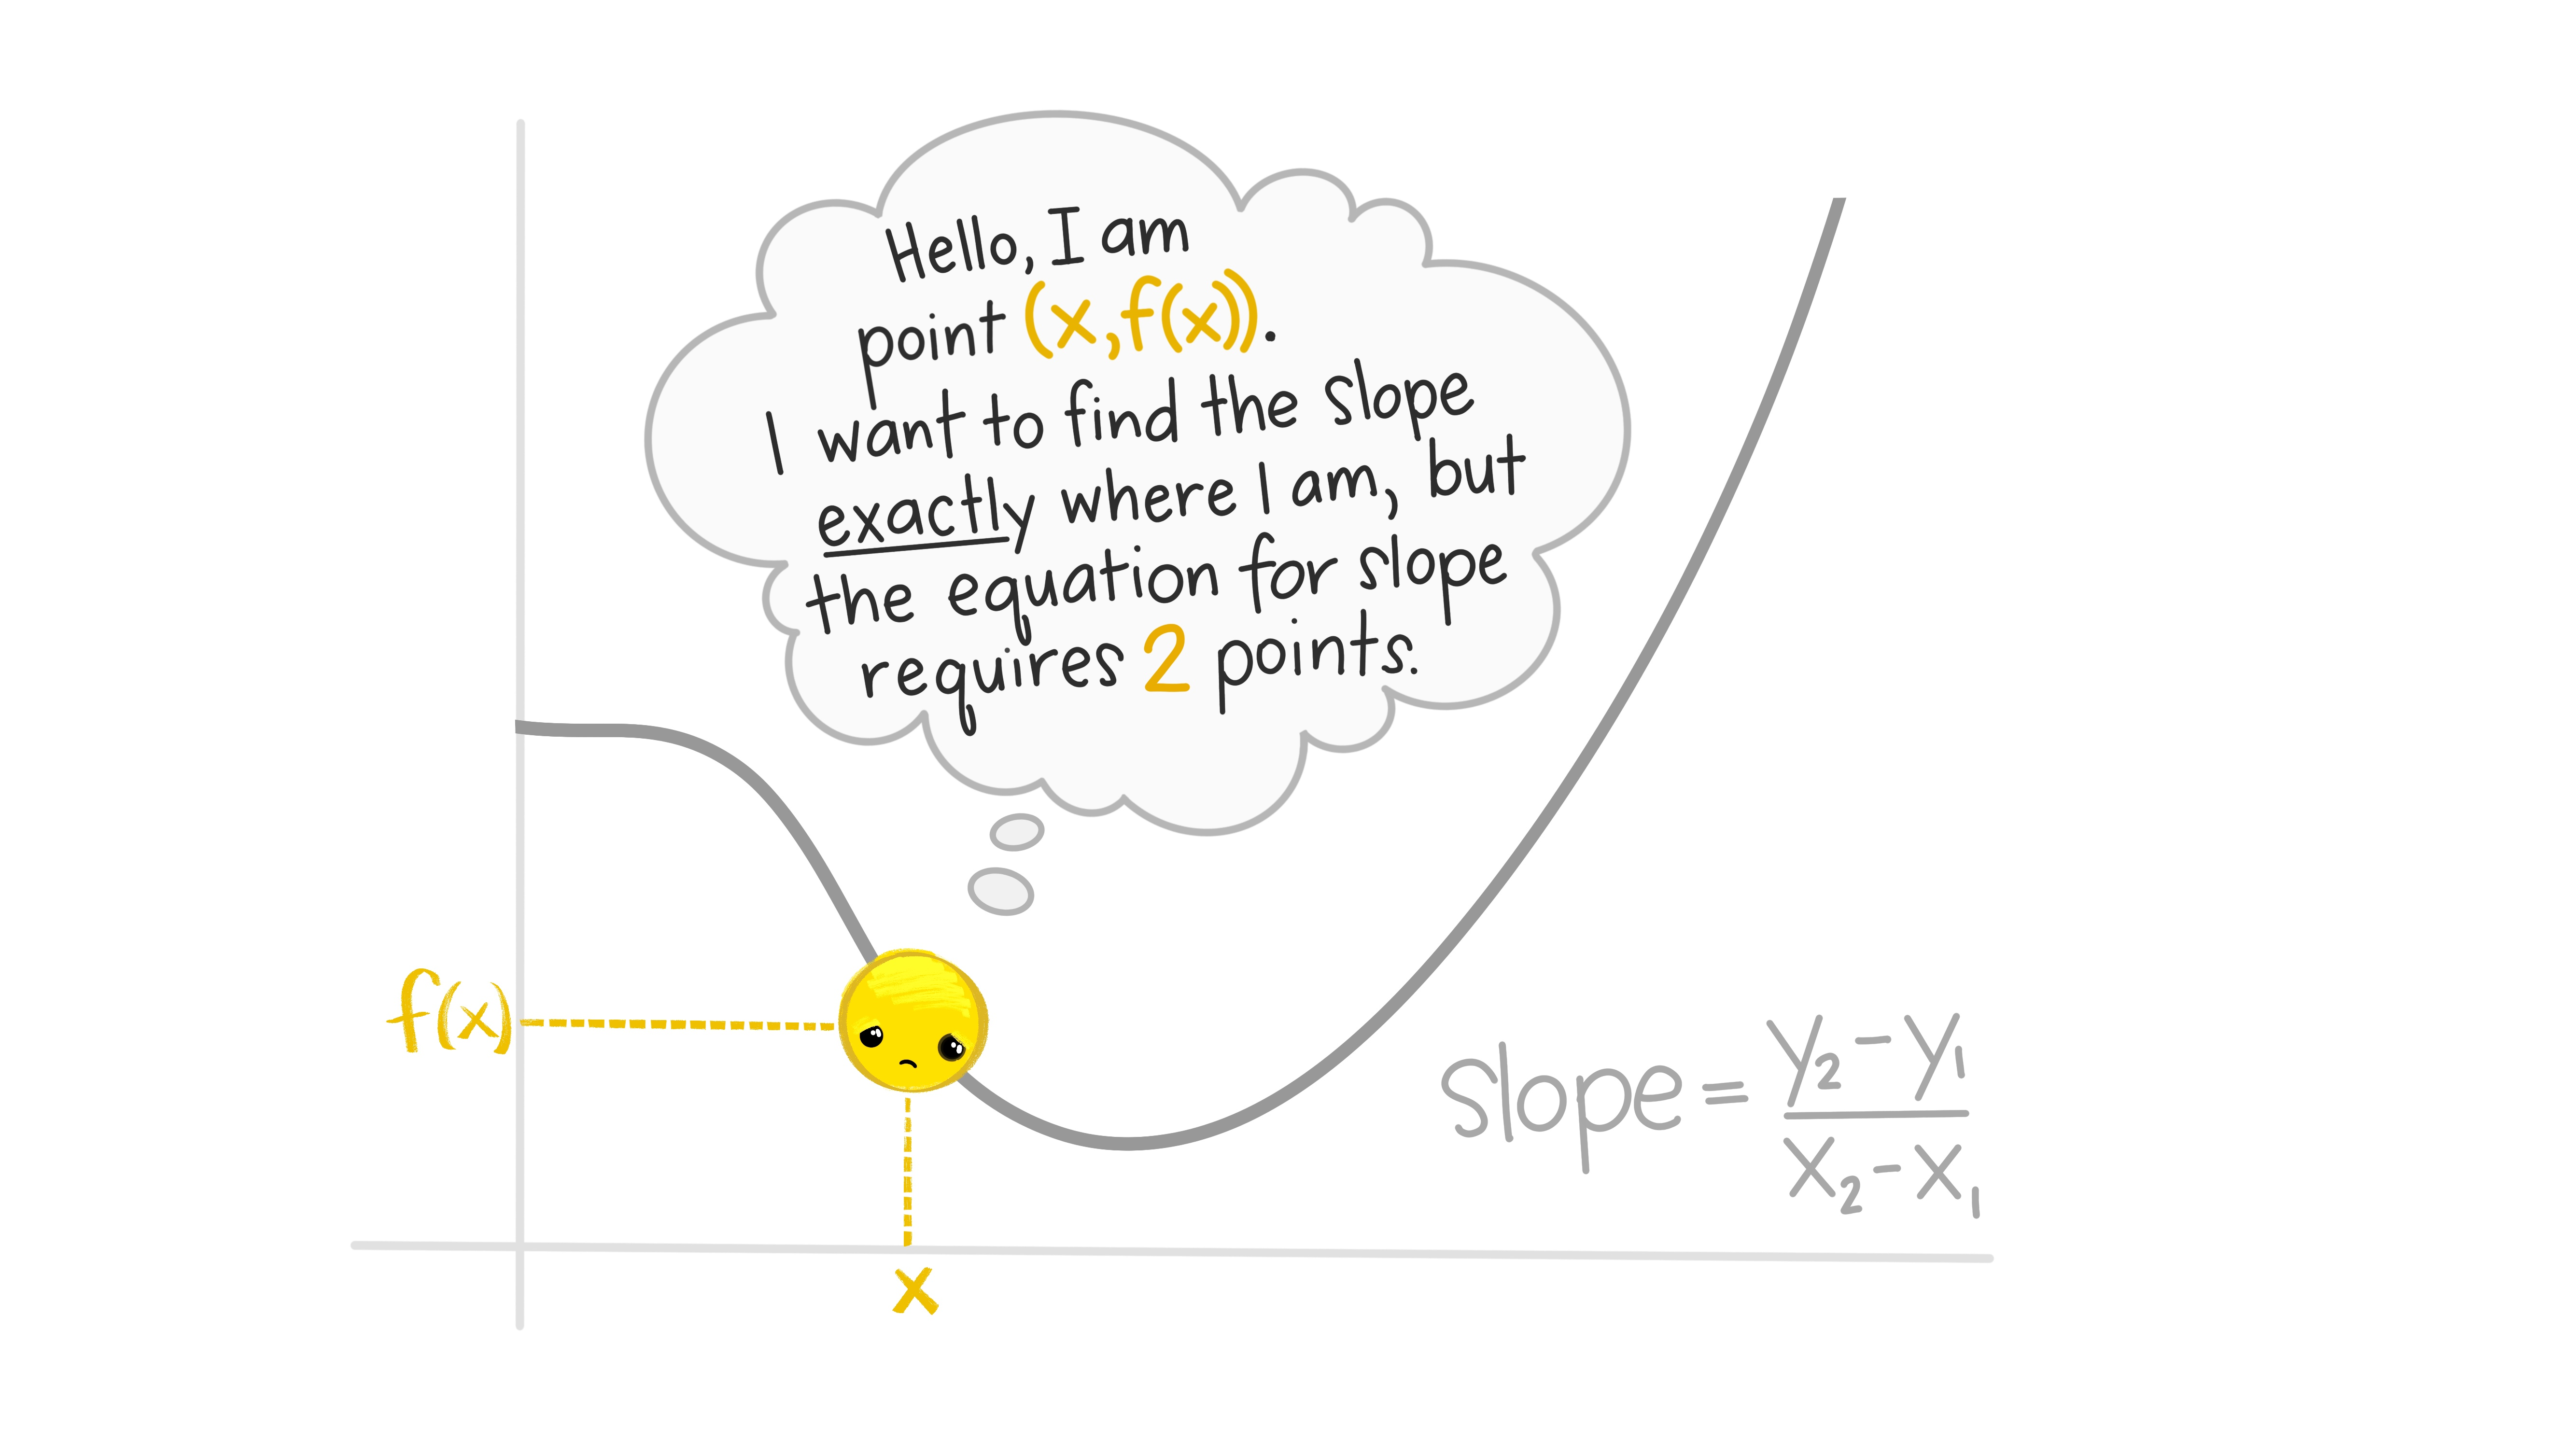
\includegraphics{extfiles/derivative_1.jpg}
\caption{Illustrating a Derivative: Artwork by '@'allison\_horst}
\end{figure}

Nowadays learning R by example is easy to do, with so many free online resources available to do so.

\begin{figure}
\centering

\includegraphics{extfiles/monster_support.jpg}
\caption{Illustrating learning R online: Artwork by '@'allison\_horst}
\end{figure}

I recomend that you do it via the RStudio environment, since it provides an integrated environment to integrate with all R things. And there are many! And if you do so, I can guarantee that in no time you will be having funR.

\begin{figure}
\centering

\includegraphics{extfiles/r_first_then.png}
\caption{Illustrating having funR: Artwork by '@'allison\_horst}
\end{figure}

The advantages of mastering R are priceless, but the learning curve can be daunting at first.

\begin{figure}
\centering
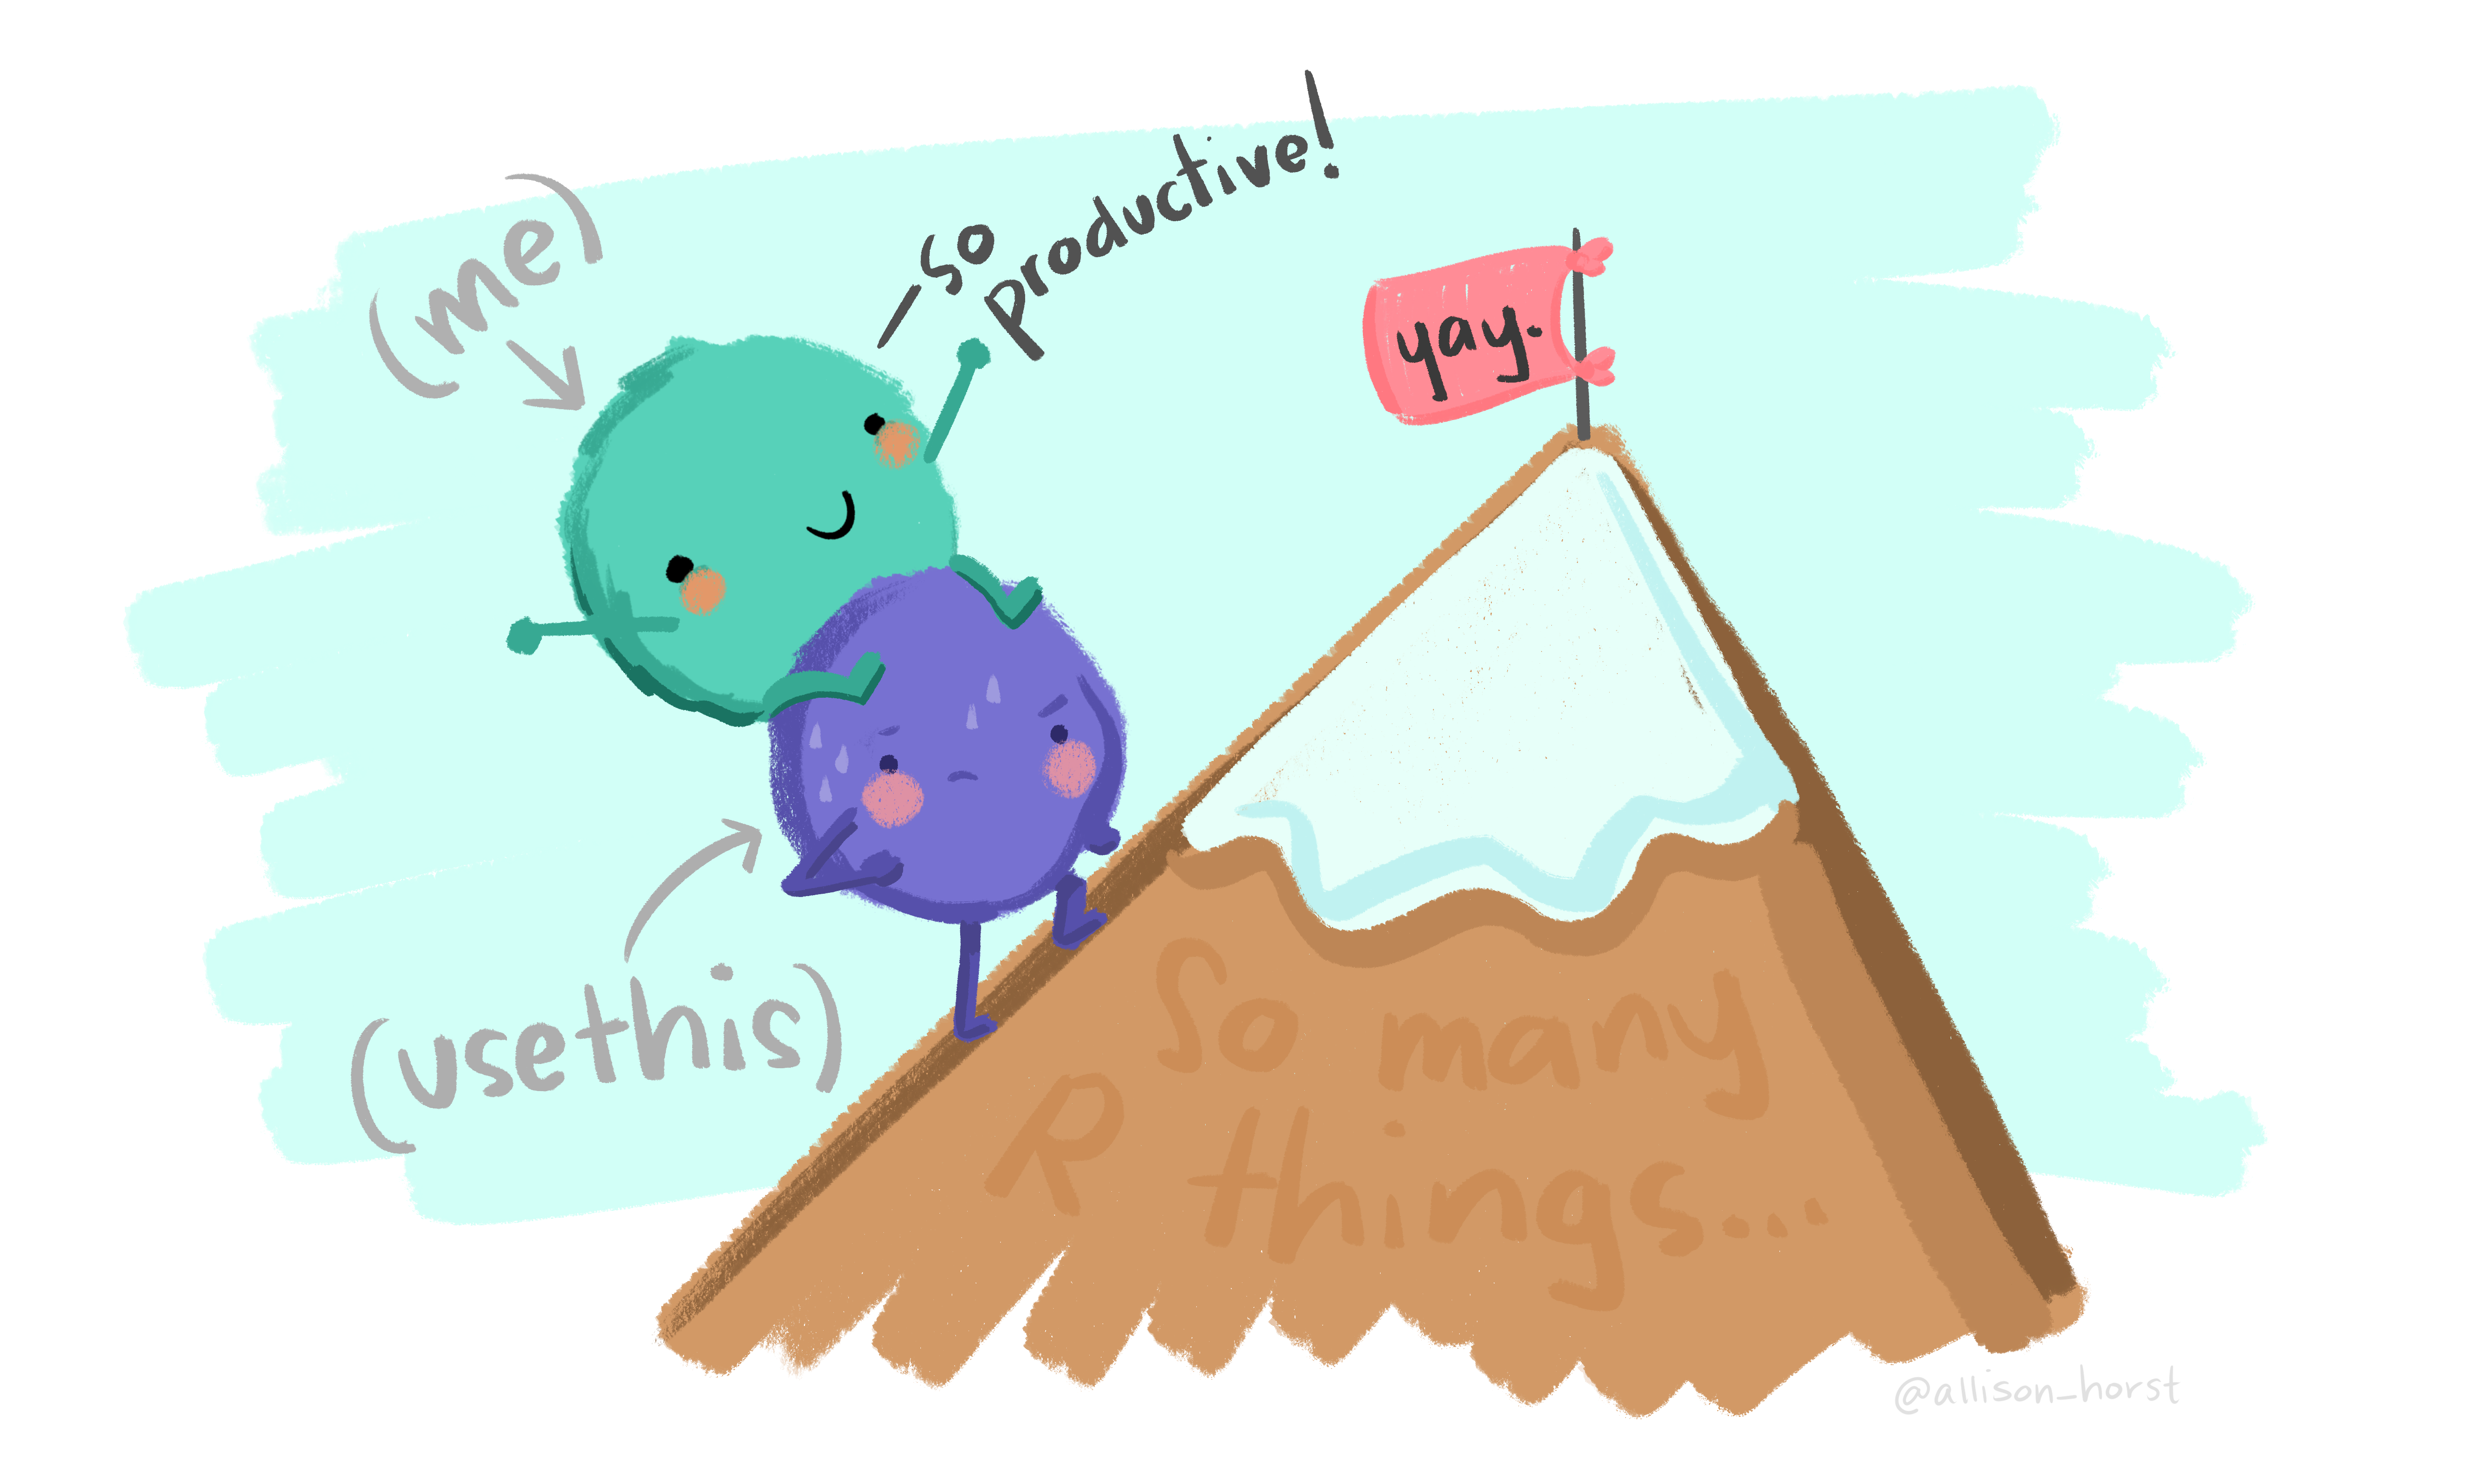
\includegraphics{extfiles/usethis.png}
\caption{Illustrating R's learning curve: Artwork by '@'allison\_horst}
\end{figure}

If you want a gentle tutorial into R I have set up such a resource here:

\url{https://github.com/TiagoAMarques/AnIntro2RTutorial}

Additionally, this book is written in bookdown, and bookdown is the 4.0 version of RMarkdown, a tool that allows you to build dynamic reports based on R code, providing integrated documents that contain all that is required for a given project, from reading the data in to final results and discussion, passing through all the analysis and results. If you want a gentle introduction to RMarkdown using a hands on tutorial based on a versatile template that will do many of the things you'll need to get started, look for no more, there is also one here:

\url{https://github.com/TiagoAMarques/RMarkdownTemplate}

Actually, since this book is a bookdown book, you can easily look at it too. It is also on github:

\url{https://github.com/TiagoAMarques/ECOMODbook}

Go out and explore, little grasshopper. You will conquer many great things if you do. You will become a code giant one day. But never forget, you need to be thankful to an entire community, and you are standing on the shoulders of giants!

\begin{figure}
\centering
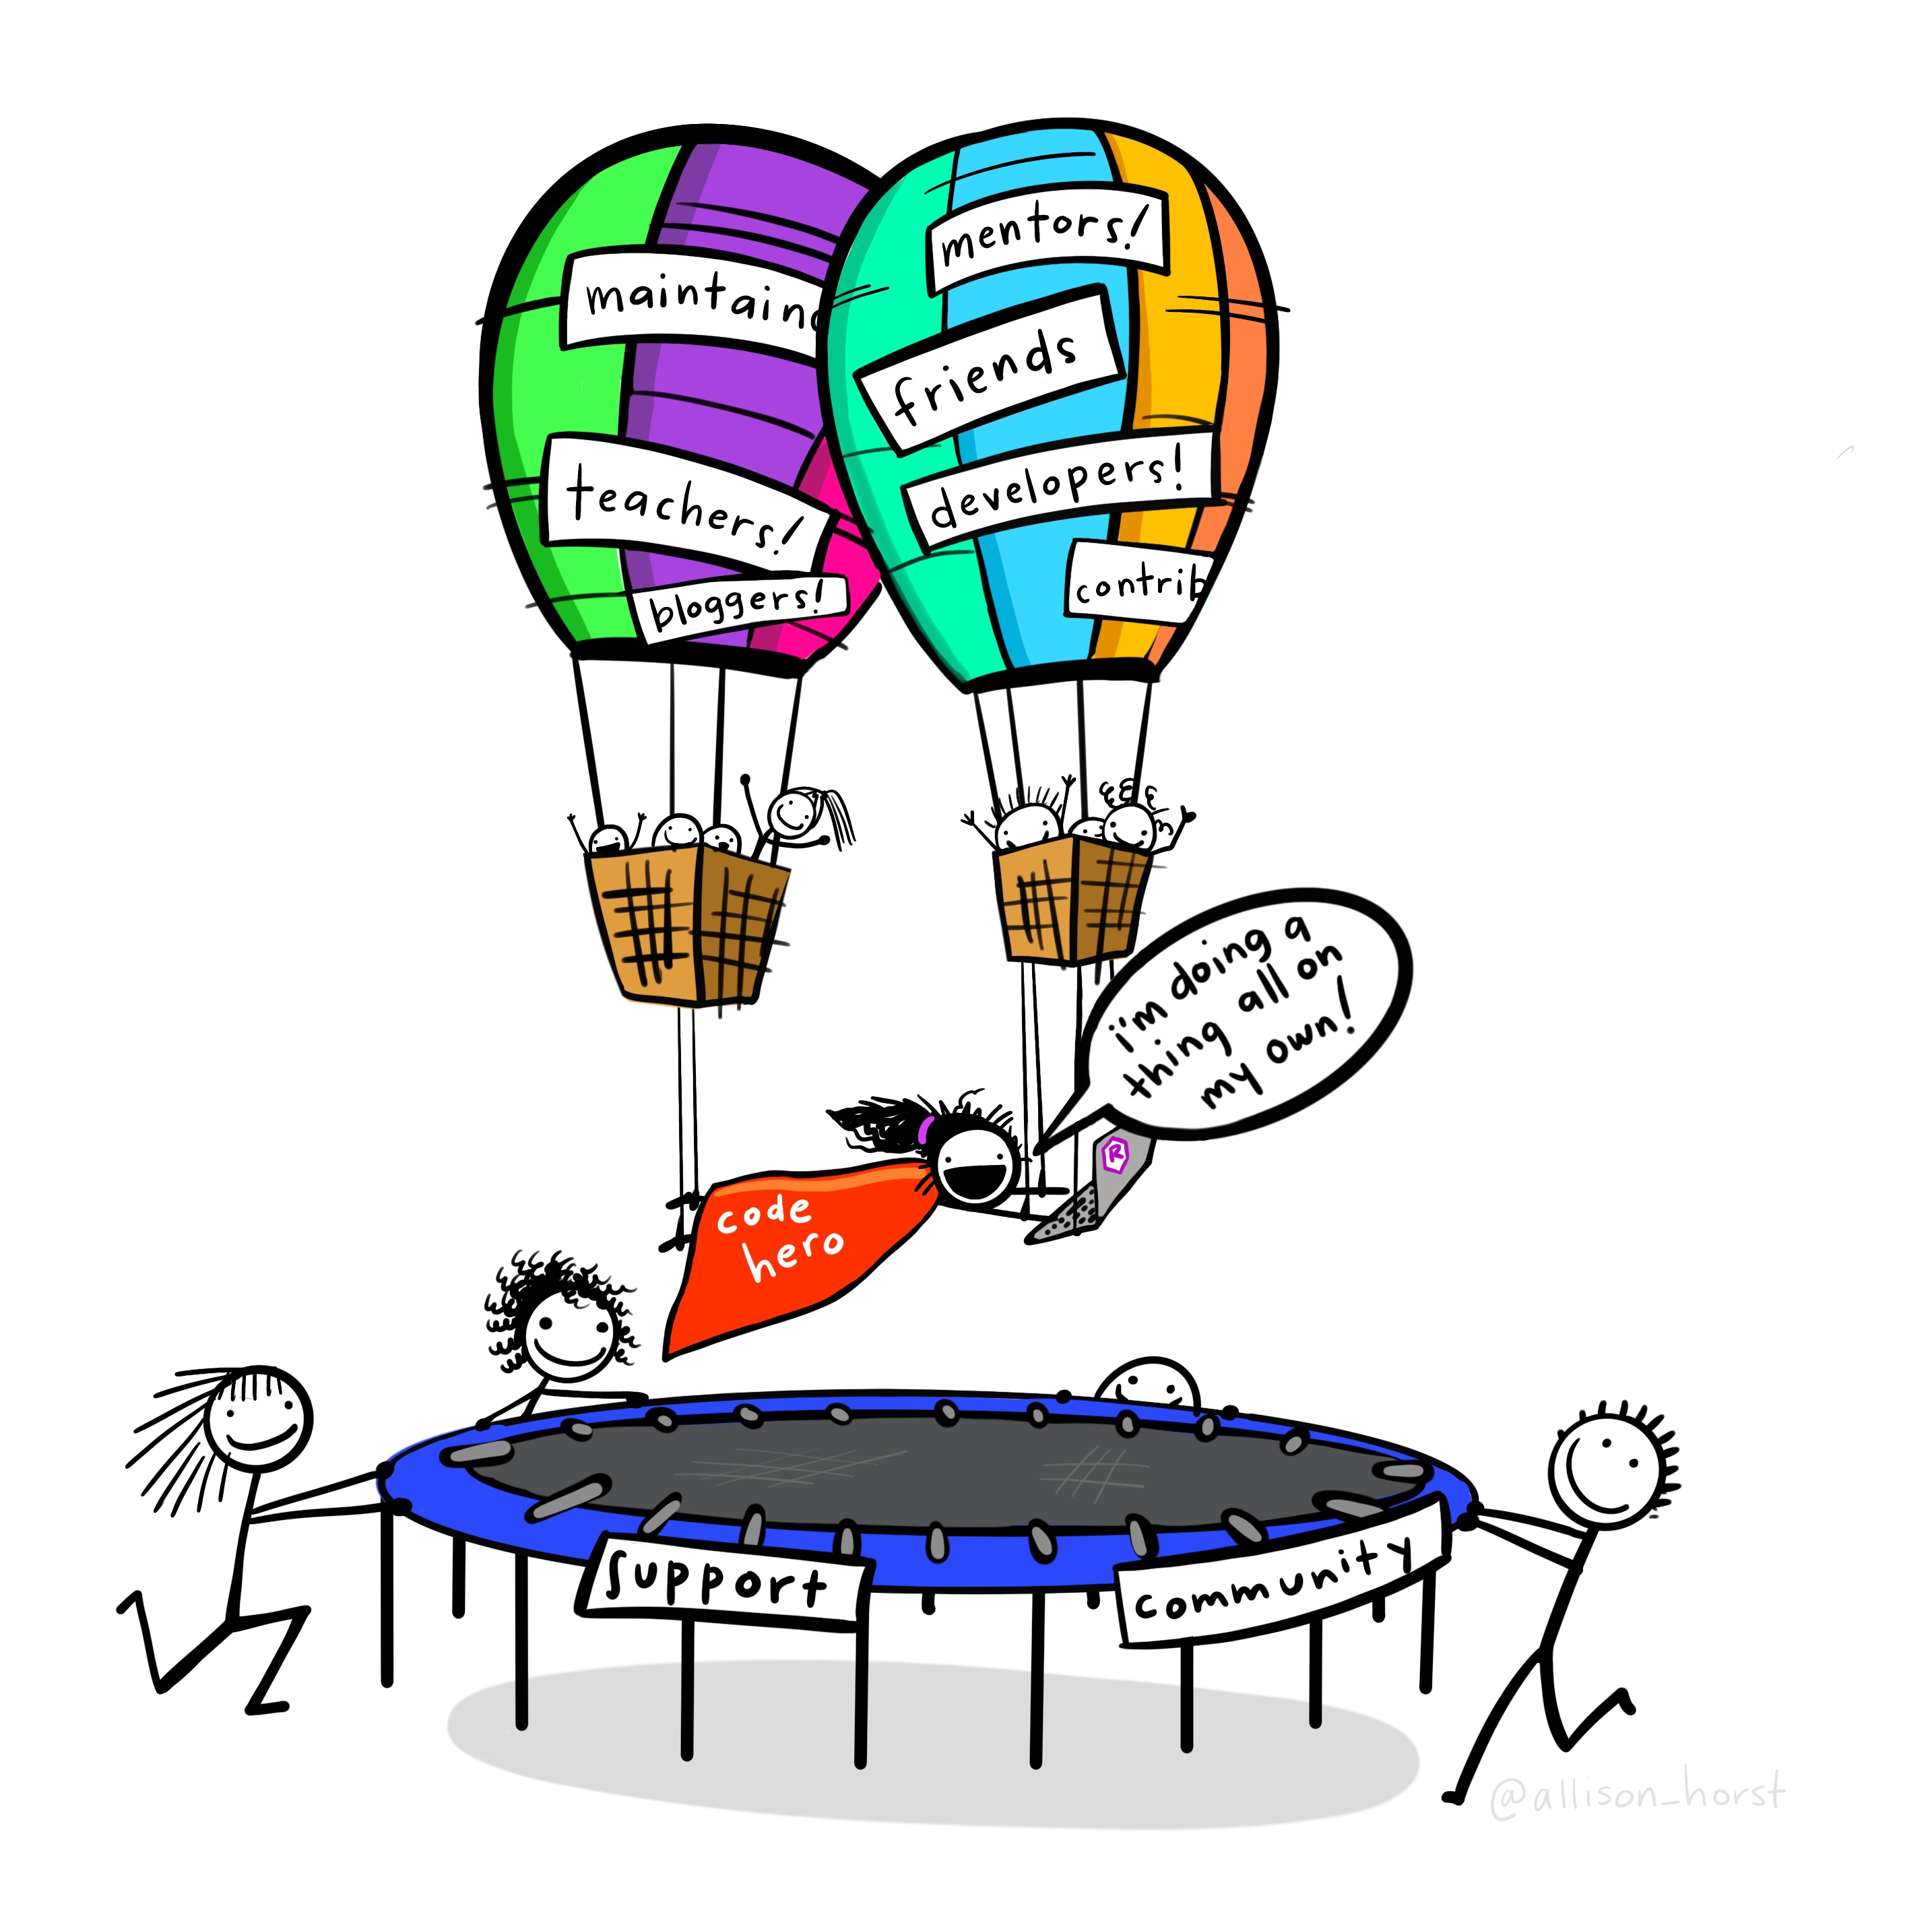
\includegraphics{extfiles/code_hero.jpg}
\caption{Illustrating standing on the shoulders of giants: Artwork by '@'allison\_horst}
\end{figure}

\hypertarget{prelim}{%
\chapter{Preliminaries}\label{prelim}}

These are fundamental references that I think any candidate to be an ecological statistician, even before being an ecological modeller, should know about. These are useful either for someone that develops methods to be used by practicioners, as well as for practitioners wanting to use the methods. Many of these are actually useful for both sets of people.

\begin{itemize}
\item
  \citet{Hurlbert1984} introduces the concept of pseudoreplication in the context of ecological field experiments. This is an ecology classic and a fundamental paper because I suspect many of th emisconceptions around the use of statistics in ecology stem from the fact that researchers try to apply methods that were developed in a context of designed experiments but in fact most ecological studies are observational in nature. Therefore, to soem degree, there is always a degree of pseudo-replication in field observations. Understanding when we can ignore these and treat observations as independent, versus when must account for that correlation in the analysis, is a fundamental ability. Unfortunately, I would say this is much easier said than done, and the ability to do so does not come in books. It is fundamentally obtained through experience.
\item
  \citet{AND2001} discuss the need to avoid index values, or in other words, that we must account for detectability when interpreting coundsof detected animals, and the fundamental avoiding convenience sampling when sampling wildlife. What you learn from sampling animals from a road in not something about the animals, but about what the animals do near roads. Understanding when the two might be, and even more important, when they might not be, the same thing, is fundamental.
\item
  \citet{Kass2016} present 10 principles for effective statistical analysis, and while they are all important, I think that the plea for being careful about the data (after all, garbage in. garbage out) and also for aiming to have reproducible analysis are key, often overlooked, messages for all researchers, and that includes those hoping to strive in ecological modelling.
\item
  \citet{King2014} reviews what is modern statitical ecology.
\item
  \citet{Gimenez2014}, along similar lines of \citet{King2014}, put forward the idea that ecological statistics is finally a ripe research field and describe the key topics and methods involved at the interface between ecology and statistics.
\item
  Martinez-Abrain2007 reminds us of how many questions about whether differences exist between two populations are non-sensical. Of course there are, and the only uqestion then becoames if we manage to gather a large enough sample size to establish them statistically. Of course, that in itself migh not mean much.
\item
  \citet{Martinez-Abrain2008} goes on and therefore discusses a fundamental aspect that we must never forget, statistical significance does not imply biological relevance.
\item
  \citet{Nakagawa2007} provide an excelent review of the concepts around effect size, confidence interval and statistical significance. These represent cornerstones of statistics that must be mastered by the ecological statistician.
\item
  \citet{OHara2010} and why you should avoid using the log of count data (which is not the same as not using log transformations, these might be useful under many contexts)
\item
  \citet{Zuur2009} is a good read about startegies to avoid the most common statistical problems (this paper was a guest paper for the first issue of the Methods in ecology and Evolution journal)
\item
  \citet{Zuur2016} a follow up paper about what to present as outputs in a regression analysis
\item
  \citet{Fourcade2017} is a cautionary tale about how using variables that are unrelated to a given spatila phenomena can induce us to think that they are causing the phenomena; in fact association might be induced by spatial autocorrelation patterns present in predictors that a (too much) efficient method might pick up.
\item
  \citet{Steel2013} presents 18 pitfalls, and ways to avoid them, when using statistics in ecology, in other words, when doing ecological statistics.
\end{itemize}

\hypertarget{about-regression}{%
\chapter{About regression}\label{about-regression}}

Some references woth looking into.

An intro to R: \citep{Zuur2009a}

Models for ecological data: \citep{Zuur2007}

More on regression and extending the linear model (just an example): \citep{Faraway2006}\citep{Zuur2009b}

\hypertarget{what-is-a-regression}{%
\section{What is a regression?}\label{what-is-a-regression}}

Where does the word come from? Gauss and regression towards the mean.

A regression is a model that allows us to predict a response variable \(y\) (a.k.a the dependent variable, because it depends on the other variables) as a function of the values ofindependent variables (a.k.a. covariates, predictors or explanatory).

\hypertarget{the-general-linear-model}{%
\section{The general linear model}\label{the-general-linear-model}}

A general expression for a regression model (i.e.~the expression for a generalized linear model is)

\[ f[E(Y|X)] = \mu = \beta_0+\beta_1 x_1 + ... + \beta_k x_k \]
where \(f\) is a function - also known as the \textbf{link function} - that links the mean value of the response, conditional on the value of the predictors, to the \textbf{linear predictor} \(\beta_0+\beta_1 x_1 + ... + \beta_k x_k\) (\(\mu\), a linear function of \(k\) covariates). In general books tend to represent this as

\[ E(Y|X) =  f^{-1}(\beta_0+\beta_1 x_1 + ... + \beta_k x_k) \]
i.e., where what is shown is the inverse of the link function,
and sometimes the notation ignores the formal conditioning on the values of the covariates

\[ E(Y) =  f^{-1}(\beta_0+\beta_1 x_1 + ... + \beta_k x_k) \]

Because this is a model, for any given observation we have

\[ f{(y_i|x_i)} =  \beta_0+\beta_1 x_{1i} + ... + \beta_k x_{ki} + e_i \]

where the \(e_i\) represents the residual (a.k.a. the error).

Most people are used to see the representation when the link function is the identity and hence

\[ y_i =  \beta_0+\beta_1 x_{1i} + ... + \beta_k x_{ki} + e_i \]

The simplest form of a generalized linear model is that where there is only one predictor, the link function is the identity and the error is Gaussian (or normal). Note that is the usual simple linear regression model

\[y_i=a+bx_i+e_i\]
with residuals

\[e_i=y_i - (a+bx_i)= y_i-\hat y_i\]

being Gaussian, i.e.~\(e_i\)\textasciitilde Gau(0,\(\sigma\)), and where the link function is the identity (i.e.~\(f(E(y))=1 \times E(y)=E(y)\)).

\hypertarget{handson}{%
\chapter{Hands On Regression}\label{handson}}

Here we come up wit a story\ldots{} an example about regression.

A simple regression is just the situation where we want to model a response variable as a function of a single explanatory variable. As an examples, say, the time a fish takes to react to a predator introduced in an aquarium by getting into shelter, as a function of the water temperature. Let's simulate some data that would represent this scenario, but I am not showing you the way the data was simulated just yet.

Nonetheless, let me tell you that the reaction times were created in object \texttt{react}, the temperatures in object \texttt{temp}, and these were then packed as a \texttt{data.frame} called \texttt{reaction}.

The first few lines of the simulated data are shown in Table \ref{tab:Ttab1}.

\begin{Shaded}
\begin{Highlighting}[]
\NormalTok{knitr}\SpecialCharTok{::}\FunctionTok{kable}\NormalTok{(}
  \FunctionTok{head}\NormalTok{(reaction, }\DecValTok{5}\NormalTok{), }\AttributeTok{caption =} \StringTok{\textquotesingle{}The simulated dataset\textquotesingle{}}\NormalTok{,}
  \AttributeTok{booktabs =} \ConstantTok{TRUE}
\NormalTok{)}
\end{Highlighting}
\end{Shaded}

\begin{table}

\caption{\label{tab:Ttab1}The simulated dataset}
\centering
\begin{tabular}[t]{rr}
\toprule
react & temp\\
\midrule
3.864305 & 11.84882\\
6.002570 & 17.02374\\
5.400667 & 15.73326\\
4.462596 & 11.68052\\
6.689445 & 19.43839\\
\bottomrule
\end{tabular}
\end{table}

The data is shown in figure \ref{fig:Freg}.

\begin{Shaded}
\begin{Highlighting}[]
\FunctionTok{par}\NormalTok{(}\AttributeTok{mar =} \FunctionTok{c}\NormalTok{(}\DecValTok{4}\NormalTok{, }\DecValTok{4}\NormalTok{, .}\DecValTok{1}\NormalTok{, .}\DecValTok{1}\NormalTok{))}
\FunctionTok{plot}\NormalTok{(react}\SpecialCharTok{\textasciitilde{}}\NormalTok{temp,}\AttributeTok{xlab=}\StringTok{"Temperature (degrees, Celcius)"}\NormalTok{,}\AttributeTok{ylab=}\StringTok{"Reaction time (seconds)"}\NormalTok{)}
\end{Highlighting}
\end{Shaded}

\begin{figure}

{\centering 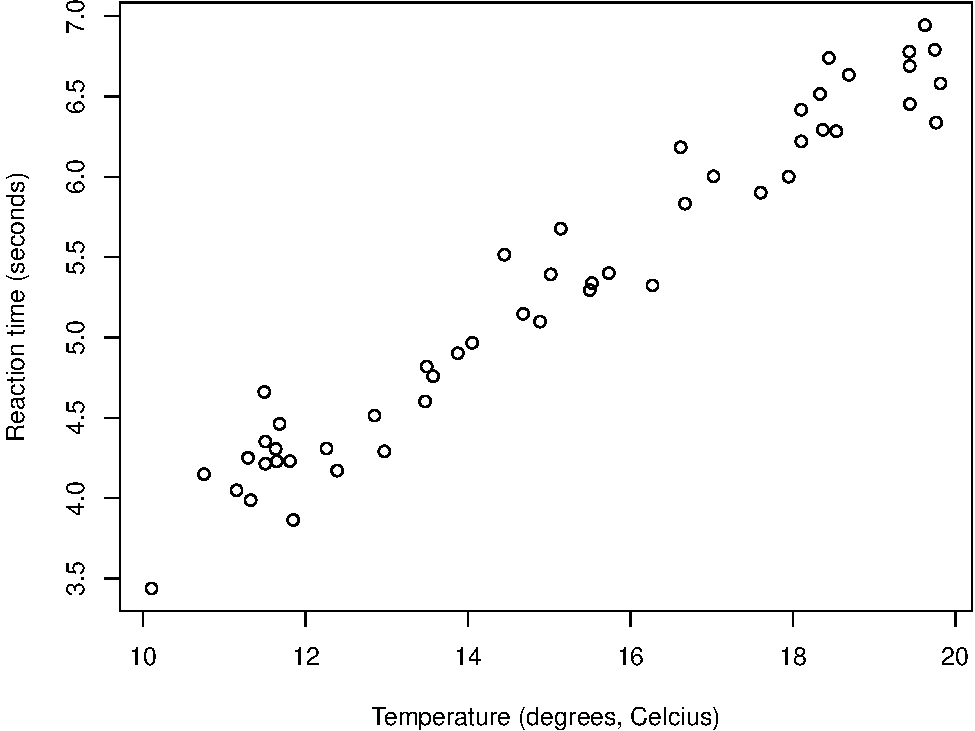
\includegraphics[width=0.8\linewidth]{ECOMODbook_files/figure-latex/Freg-1} 

}

\caption{An example regression data set that could be eplained by a linear regression}\label{fig:Freg}
\end{figure}

It seems like there is a linear relationship between the predictor (temperature) and the response (the reaction time). We could therepore model it with a simple linear regression. We can do that using R´s function \texttt{lm}. We do so here and then look at the summary of the object produced.

The required argument for \texttt{lm} is the \texttt{formula} that defines the regression model. The symbol \texttt{\textasciitilde{}}is used to represent ``as a function of''. So here we will want something like ``reaction time \textasciitilde{} water temperature''.

While this might seem like a detail, it is a good policy to always fit models using explicitly the \texttt{data} argument, instead of fitting the model to objects hanging around the workspace. Learn how to be tidy!

Therefore, while the imideate result would be the same, we suggest that you do not do this

\begin{Shaded}
\begin{Highlighting}[]
\NormalTok{mod0}\OtherTok{\textless{}{-}}\FunctionTok{lm}\NormalTok{(react}\SpecialCharTok{\textasciitilde{}}\NormalTok{temp)}
\end{Highlighting}
\end{Shaded}

nor this

\begin{Shaded}
\begin{Highlighting}[]
\NormalTok{mod0}\OtherTok{\textless{}{-}}\FunctionTok{lm}\NormalTok{(reaction}\SpecialCharTok{$}\NormalTok{react}\SpecialCharTok{\textasciitilde{}}\NormalTok{reaction}\SpecialCharTok{$}\NormalTok{temp)}
\end{Highlighting}
\end{Shaded}

but always consider this

\begin{Shaded}
\begin{Highlighting}[]
\NormalTok{mod0}\OtherTok{\textless{}{-}}\FunctionTok{lm}\NormalTok{(react}\SpecialCharTok{\textasciitilde{}}\NormalTok{temp,}\AttributeTok{data=}\NormalTok{reaction)}
\FunctionTok{summary}\NormalTok{(mod0)}
\end{Highlighting}
\end{Shaded}

\begin{verbatim}
## 
## Call:
## lm(formula = react ~ temp, data = reaction)
## 
## Residuals:
##      Min       1Q   Median       3Q      Max 
## -0.43172 -0.13223 -0.01381  0.13843  0.49265 
## 
## Coefficients:
##             Estimate Std. Error t value Pr(>|t|)    
## (Intercept)  0.55487    0.15642   3.547 0.000881 ***
## temp         0.31442    0.01015  30.986  < 2e-16 ***
## ---
## Signif. codes:  0 '***' 0.001 '**' 0.01 '*' 0.05 '.' 0.1 ' ' 1
## 
## Residual standard error: 0.2182 on 48 degrees of freedom
## Multiple R-squared:  0.9524, Adjusted R-squared:  0.9514 
## F-statistic: 960.2 on 1 and 48 DF,  p-value: < 2.2e-16
\end{verbatim}

This will be easier to read for others, makes you tidy, and will save you headaches when using functions like \texttt{predict} over the resulting fitted model.

We can the estimated regression line to the above plot. I color it red to remind us of the fact that this is an estimated line, not the true line that generated the data. While in general we do not know this with real data, here I know the model that was used to simulate the data. Just for comparison I can add it to the plot to compare with the estimated regression line.

\begin{Shaded}
\begin{Highlighting}[]
\FunctionTok{plot}\NormalTok{(react}\SpecialCharTok{\textasciitilde{}}\NormalTok{temp,}\AttributeTok{xlab=}\StringTok{"Temperature (degrees, Celcius)"}\NormalTok{,}\AttributeTok{ylab=}\StringTok{"Reaction time (seconds)"}\NormalTok{)}
\FunctionTok{abline}\NormalTok{(mod0,}\AttributeTok{lty=}\DecValTok{2}\NormalTok{,}\AttributeTok{col=}\StringTok{"red"}\NormalTok{)}
\FunctionTok{abline}\NormalTok{(beta0,beta1,}\AttributeTok{lty=}\DecValTok{2}\NormalTok{,}\AttributeTok{col=}\StringTok{"green"}\NormalTok{)}
\FunctionTok{legend}\NormalTok{(}\StringTok{"topleft"}\NormalTok{,}\AttributeTok{legend=}\FunctionTok{c}\NormalTok{(}\StringTok{"Real model"}\NormalTok{,}\StringTok{"Estimated Regression Line"}\NormalTok{),}\AttributeTok{col=}\FunctionTok{c}\NormalTok{(}\StringTok{"green"}\NormalTok{,}\StringTok{"red"}\NormalTok{),}\AttributeTok{lty=}\DecValTok{2}\NormalTok{, }\AttributeTok{inset=}\FloatTok{0.05}\NormalTok{)}
\end{Highlighting}
\end{Shaded}

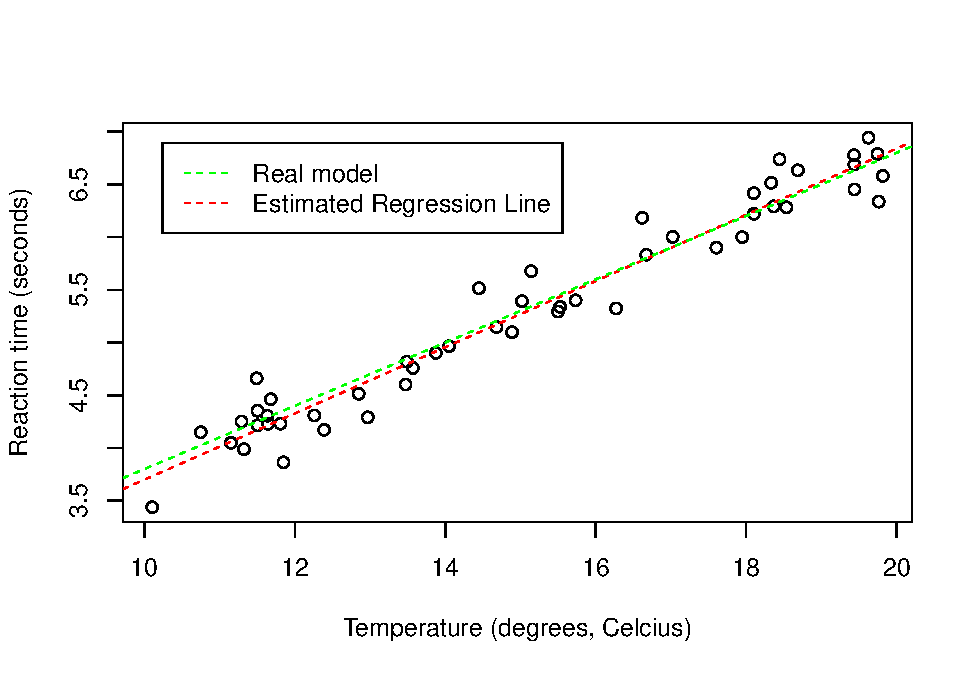
\includegraphics{ECOMODbook_files/figure-latex/reg9-1.pdf}

The estimated line and the true line are very similar, as expected since we have a reasonable sample size, a small error, and a model that is the reality. With real data, this will be the exception, not the rule. All models are wrong, but some are useful. The linear regression model is perhaps one of the simplest, but also one of the most widely used, and hence, one of those that has been extremely useful. But of course, its simplicity is also its major disadvantage, as we shall see.

\hypertarget{the-assumptions-are-on-the-residuals-not-the-data}{%
\section{The assumptions are on the residuals, not the data}\label{the-assumptions-are-on-the-residuals-not-the-data}}

Imagine that you have a single variable that you are interested in modelling. This is the concentration of an enzime in the blood of small rodents, from 4 diffferent species. This is represented in the image below \ref{fig:figrodents}.

\begin{Shaded}
\begin{Highlighting}[]
\FunctionTok{hist}\NormalTok{(ys,}\AttributeTok{breaks=}\DecValTok{0}\SpecialCharTok{:}\DecValTok{40}\NormalTok{,}\AttributeTok{xlab=}\StringTok{"Concentration of enzime (mg/L)"}\NormalTok{)}
\end{Highlighting}
\end{Shaded}

\begin{figure}

{\centering 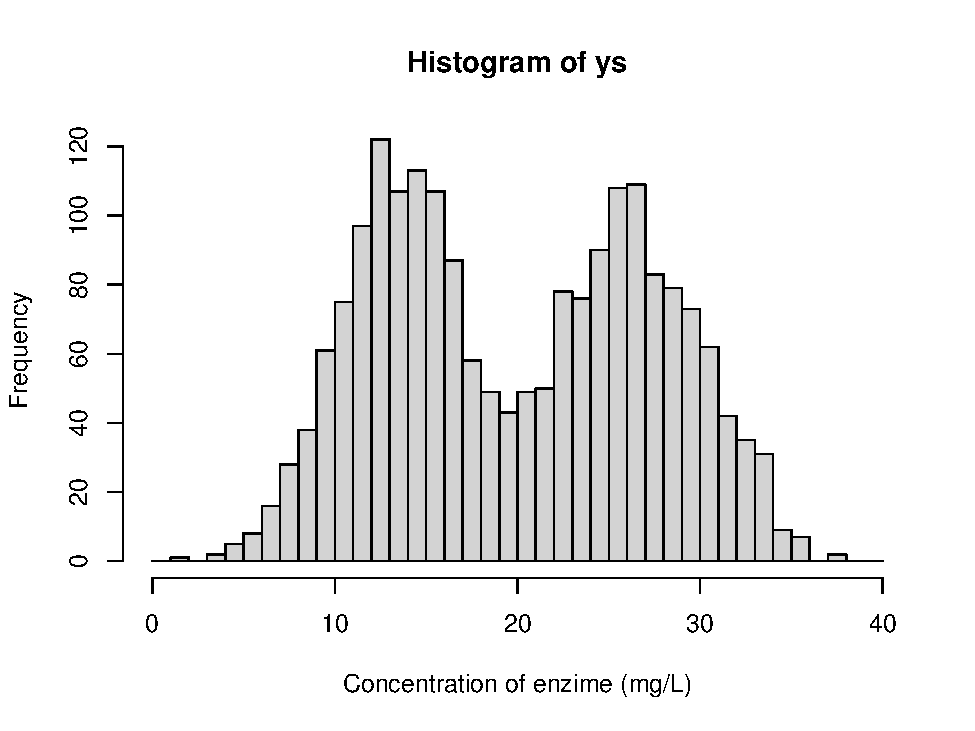
\includegraphics[width=0.8\linewidth]{ECOMODbook_files/figure-latex/figrodents-1} 

}

\caption{Concentration of an enzime (mg/L) in the blood of small rodents, from 4 diffferent species}\label{fig:figrodents}
\end{figure}

A poor (conventional and traditional) biologist would die if shown this dataset, but the truth is there would be no reason for it. If one accounts for the different species, this is what we see. Clear differences between two groups of species.

\begin{Shaded}
\begin{Highlighting}[]
\FunctionTok{boxplot}\NormalTok{(ys}\SpecialCharTok{\textasciitilde{}}\NormalTok{type,}\AttributeTok{ylab=}\StringTok{"Concentration of enzime (mg/L)"}\NormalTok{)}
\end{Highlighting}
\end{Shaded}

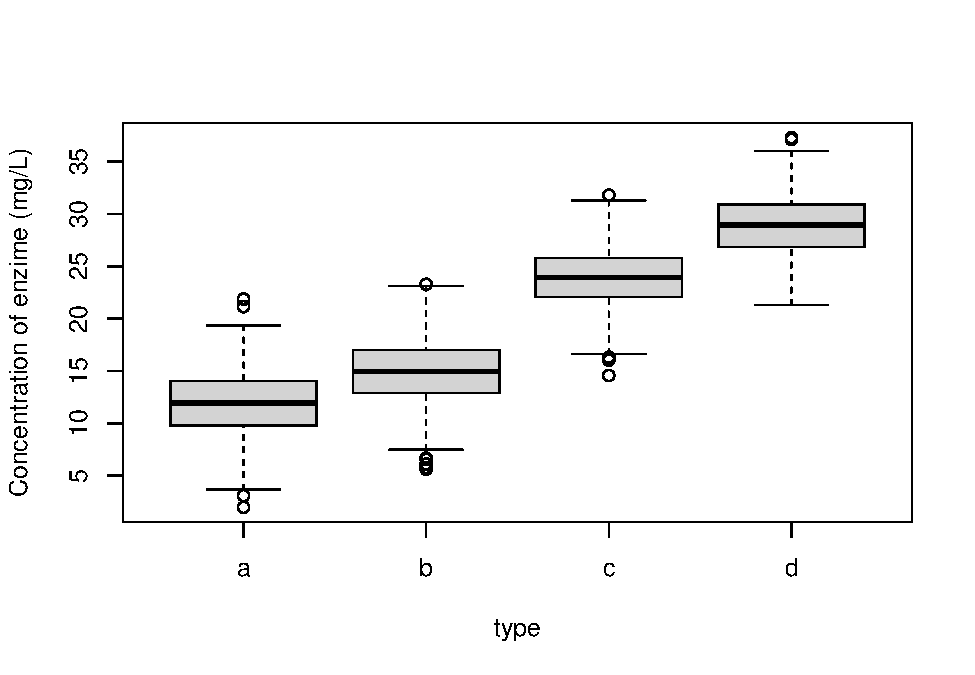
\includegraphics{ECOMODbook_files/figure-latex/reg11-1.pdf}

And further, we can see that the remaining residuals are a beautiful Gaussian. Not a surprise, since this was simulated data, from a Gaussian model :) !

\begin{Shaded}
\begin{Highlighting}[]
\FunctionTok{hist}\NormalTok{(}\FunctionTok{residuals}\NormalTok{(}\FunctionTok{lm}\NormalTok{(ys}\SpecialCharTok{\textasciitilde{}}\NormalTok{type)),}\AttributeTok{main=}\StringTok{""}\NormalTok{,}\AttributeTok{xlab=}\StringTok{"Residuals"}\NormalTok{)}
\end{Highlighting}
\end{Shaded}

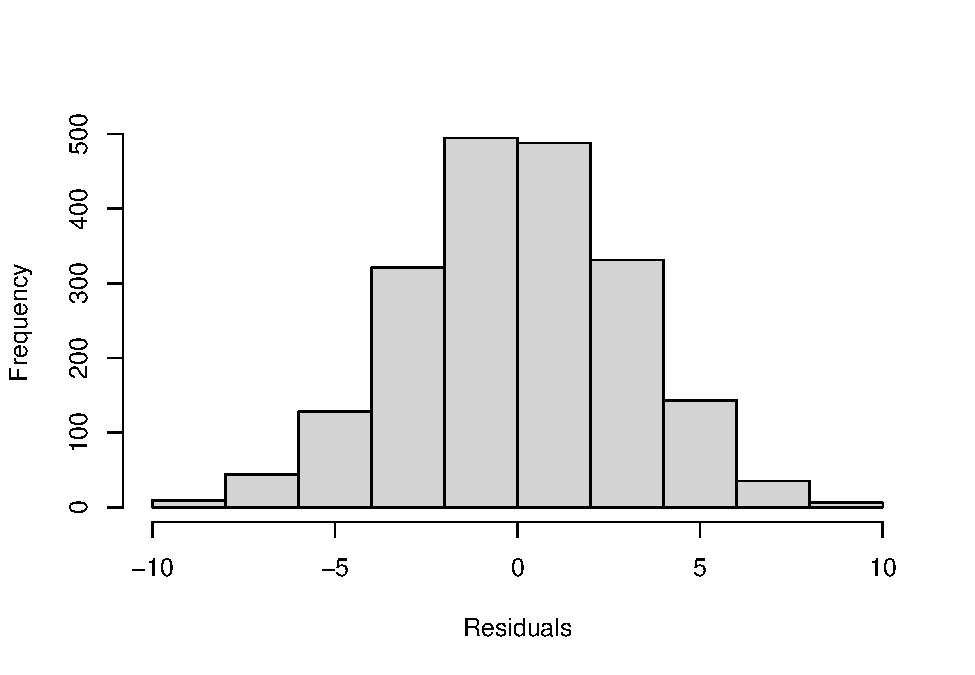
\includegraphics{ECOMODbook_files/figure-latex/reg12-1.pdf}

The take home message from the story: what the data looks like might be irrelevant. The patterns that remain in the residuals, if any, those are the ones we might need to worry about. So do not transform data just becasue the data looks odd. It might just be Gaussian data in disguise!

\hypertarget{aula6}{%
\chapter{Class 6 13 10 2020}\label{aula6}}

\hypertarget{implementing-a-regression}{%
\section{Implementing a regression}\label{implementing-a-regression}}

We begin by reading the data in ``lagartos.txt'' and fitting a regression model to it.

Read the data in

\begin{Shaded}
\begin{Highlighting}[]
\CommentTok{\#folder\textless{}{-}"../Aula6 13 10 2020/"}
\NormalTok{folder}\OtherTok{\textless{}{-}}\StringTok{"extfiles/"}
\NormalTok{lagartos }\OtherTok{\textless{}{-}} \FunctionTok{read.csv}\NormalTok{(}\AttributeTok{file=}\FunctionTok{paste0}\NormalTok{(folder,}\StringTok{"lagartos.txt"}\NormalTok{), }\AttributeTok{sep=}\StringTok{""}\NormalTok{)}
\NormalTok{n }\OtherTok{\textless{}{-}} \FunctionTok{nrow}\NormalTok{(lagartos)}
\end{Highlighting}
\end{Shaded}

We see that we have 97 observations.

Plot the data

\begin{Shaded}
\begin{Highlighting}[]
\FunctionTok{with}\NormalTok{(lagartos,}\FunctionTok{plot}\NormalTok{(peso}\SpecialCharTok{\textasciitilde{}}\NormalTok{comp))}
\end{Highlighting}
\end{Shaded}

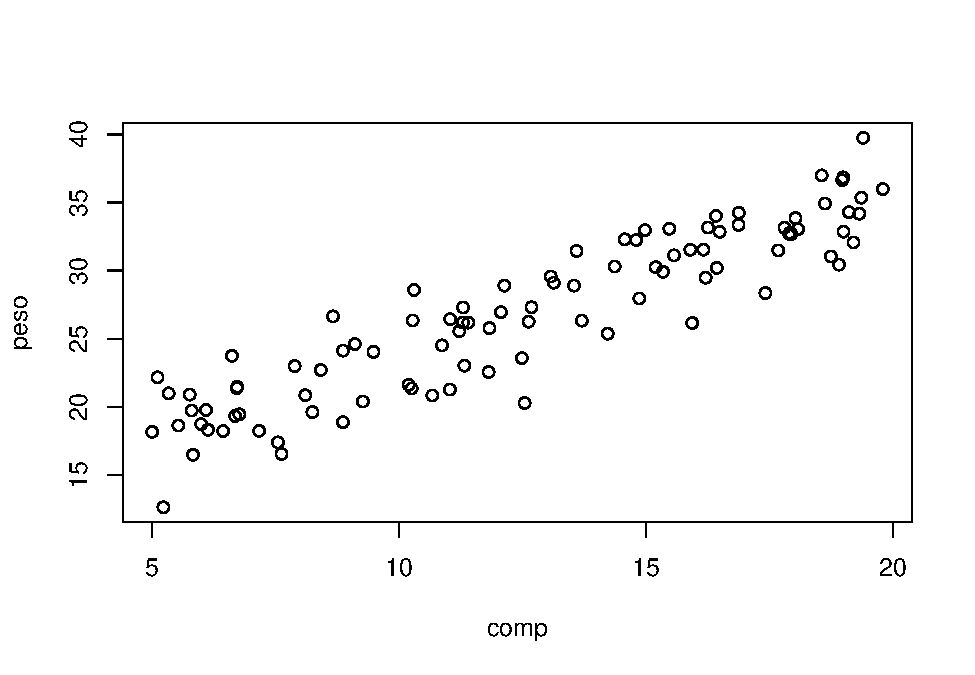
\includegraphics{ECOMODbook_files/figure-latex/a6.2-1.pdf}

A linear model seems adequate. Lets fit a regression line to the data

\begin{Shaded}
\begin{Highlighting}[]
\NormalTok{lmlag }\OtherTok{\textless{}{-}} \FunctionTok{lm}\NormalTok{(peso}\SpecialCharTok{\textasciitilde{}}\NormalTok{comp,}\AttributeTok{data=}\NormalTok{lagartos)}
\FunctionTok{summary}\NormalTok{(lmlag)}
\end{Highlighting}
\end{Shaded}

\begin{verbatim}
## 
## Call:
## lm(formula = peso ~ comp, data = lagartos)
## 
## Residuals:
##     Min      1Q  Median      3Q     Max 
## -6.5199 -1.6961  0.3495  1.7490  4.7127 
## 
## Coefficients:
##             Estimate Std. Error t value Pr(>|t|)    
## (Intercept) 11.72234    0.72299   16.21   <2e-16 ***
## comp         1.20233    0.05402   22.26   <2e-16 ***
## ---
## Signif. codes:  0 '***' 0.001 '**' 0.01 '*' 0.05 '.' 0.1 ' ' 1
## 
## Residual standard error: 2.415 on 95 degrees of freedom
## Multiple R-squared:  0.8391, Adjusted R-squared:  0.8374 
## F-statistic: 495.3 on 1 and 95 DF,  p-value: < 2.2e-16
\end{verbatim}

Remember that a linear model is just a special GLM:

\begin{Shaded}
\begin{Highlighting}[]
\NormalTok{glmlag }\OtherTok{\textless{}{-}} \FunctionTok{glm}\NormalTok{(peso}\SpecialCharTok{\textasciitilde{}}\NormalTok{comp,}\AttributeTok{data=}\NormalTok{lagartos,}\AttributeTok{family=}\FunctionTok{gaussian}\NormalTok{(}\AttributeTok{link=}\StringTok{"identity"}\NormalTok{))}
\FunctionTok{summary}\NormalTok{(glmlag)}
\end{Highlighting}
\end{Shaded}

\begin{verbatim}
## 
## Call:
## glm(formula = peso ~ comp, family = gaussian(link = "identity"), 
##     data = lagartos)
## 
## Deviance Residuals: 
##     Min       1Q   Median       3Q      Max  
## -6.5199  -1.6961   0.3495   1.7490   4.7127  
## 
## Coefficients:
##             Estimate Std. Error t value Pr(>|t|)    
## (Intercept) 11.72234    0.72299   16.21   <2e-16 ***
## comp         1.20233    0.05402   22.26   <2e-16 ***
## ---
## Signif. codes:  0 '***' 0.001 '**' 0.01 '*' 0.05 '.' 0.1 ' ' 1
## 
## (Dispersion parameter for gaussian family taken to be 5.830492)
## 
##     Null deviance: 3441.8  on 96  degrees of freedom
## Residual deviance:  553.9  on 95  degrees of freedom
## AIC: 450.27
## 
## Number of Fisher Scoring iterations: 2
\end{verbatim}

as we can see the output looks a bit different (after all, \texttt{lm} and \texttt{glm} are different functions!), but the results are exactly the same. This does not prove it, but it illustrates by example that a lm is just a GLM with a Gaussian response and an \texttt{identity} link function.

Lets use the results from \texttt{lm}, while noting that everything else would be the same.

The estimated regression line is

peso =11.72 +1.2 \(\times\) comp

and the estimated R-squared is 0.84. The standard error associated with the model is estimated to be 2.4146. Below we explain what each of these values correspond to.

The estimated standard error corresponds to the standard deviation of the residuals of the model, that is, the diference between the observations and the predicted values given the model.

The observation we have already, those are the \texttt{peso}. We can obtain the predicted \texttt{peso} for each observation with the function \texttt{predict}, but here we do it manually so that we see that the errors are just the observations minus the predictions.

\begin{Shaded}
\begin{Highlighting}[]
\CommentTok{\#get estimated values}
\NormalTok{estimated}\OtherTok{\textless{}{-}}\FunctionTok{with}\NormalTok{(lagartos,}\FunctionTok{summary}\NormalTok{(lmlag)}\SpecialCharTok{$}\NormalTok{coefficients[}\DecValTok{1}\NormalTok{]}\SpecialCharTok{+}\FunctionTok{summary}\NormalTok{(lmlag)}\SpecialCharTok{$}\NormalTok{coefficients[}\DecValTok{2}\NormalTok{]}\SpecialCharTok{*}\NormalTok{comp)}
\CommentTok{\# note this would be the same as}
\CommentTok{\# estimated\textless{}{-}predict(lmlag)}
\end{Highlighting}
\end{Shaded}

Now we can compute the residuals and their corresponding standard error

\begin{Shaded}
\begin{Highlighting}[]
\CommentTok{\#get residuals}
\CommentTok{\#erros = observações {-} valores previstos}
\CommentTok{\# e= y{-} (a+bx)}
\CommentTok{\# y= (a+bx) + e}
\NormalTok{resid}\OtherTok{\textless{}{-}}\NormalTok{lagartos}\SpecialCharTok{$}\NormalTok{peso}\SpecialCharTok{{-}}\NormalTok{estimated}
\FunctionTok{sd}\NormalTok{(resid)}
\end{Highlighting}
\end{Shaded}

\begin{verbatim}
## [1] 2.402032
\end{verbatim}

Note as predict, we could use just the function \texttt{residuals} with the model object as argument to get us the residuals in a single line of code.

The reason the above standard error is not exactly the same as in the model output above has to do with the degrees of freedom, a concepth that is hard to explain in this applied context, but relates to the number of available independent bits of information available. So turst me when I say that we loose a degree of freedom for each parameter estimated in a model. The exact value of the standard deviation as estimated in the model must account for that loss of one extra degree of freedom (associated with estimating the slope of the line), and so the standard formula of the \texttt{sd} needs to be adjusted for the lost degree of freedom, like this:

\begin{Shaded}
\begin{Highlighting}[]
\CommentTok{\#Residual Standard error (Like Standard Deviation)}
\CommentTok{\#the right way}
\CommentTok{\#Subtract one to ignore intercept}
\NormalTok{k}\OtherTok{=}\FunctionTok{length}\NormalTok{(lmlag}\SpecialCharTok{$}\NormalTok{coefficients)}\SpecialCharTok{{-}}\DecValTok{1} 
\CommentTok{\#get the error sum of squares}
\NormalTok{SSE}\OtherTok{=}\FunctionTok{sum}\NormalTok{(lmlag}\SpecialCharTok{$}\NormalTok{residuals}\SpecialCharTok{**}\DecValTok{2}\NormalTok{)}
\CommentTok{\#Residual Standard Error}
\FunctionTok{sqrt}\NormalTok{(SSE}\SpecialCharTok{/}\NormalTok{(n}\SpecialCharTok{{-}}\NormalTok{(}\DecValTok{1}\SpecialCharTok{+}\NormalTok{k))) }
\end{Highlighting}
\end{Shaded}

\begin{verbatim}
## [1] 2.414641
\end{verbatim}

\begin{Shaded}
\begin{Highlighting}[]
\CommentTok{\#equivalently}
\FunctionTok{sqrt}\NormalTok{(}\FunctionTok{var}\NormalTok{(resid)}\SpecialCharTok{*}\NormalTok{(n}\DecValTok{{-}1}\NormalTok{)}\SpecialCharTok{/}\NormalTok{(n}\DecValTok{{-}2}\NormalTok{))}
\end{Highlighting}
\end{Shaded}

\begin{verbatim}
## [1] 2.414641
\end{verbatim}

Now we get the exact same value as above: 2.4146412.

The \texttt{summary} of the model above is very useful, but nothing like adding the estimated model to the plot with the data. We can easily add the line to the plot with function \texttt{abline} (tip: note the ab in \texttt{abline} correspond to the \(a\) and \(b\) in \(y=a+bx\), but the function abline is ``smart'' enough to take an object of class \texttt{lm} and extract the corresponding \(a\) and \(b\) for plotting)

\begin{Shaded}
\begin{Highlighting}[]
\CommentTok{\#with(lagartos,plot(peso\textasciitilde{}comp))}
\FunctionTok{plot}\NormalTok{(peso}\SpecialCharTok{\textasciitilde{}}\NormalTok{comp,}\AttributeTok{data=}\NormalTok{lagartos)}
\CommentTok{\#these next 3 lines are equivalent}
\FunctionTok{abline}\NormalTok{(lmlag,}\AttributeTok{col=}\StringTok{"orange"}\NormalTok{)}
\FunctionTok{abline}\NormalTok{(}\AttributeTok{a=}\FloatTok{11.72234}\NormalTok{,}\AttributeTok{b=}\FloatTok{1.20233}\NormalTok{,}\AttributeTok{col=}\StringTok{"pink"}\NormalTok{)}
\CommentTok{\# y = a + bx}
\FunctionTok{abline}\NormalTok{(}\AttributeTok{a=}\FunctionTok{summary}\NormalTok{(lmlag)}\SpecialCharTok{$}\NormalTok{coefficients[}\DecValTok{1}\NormalTok{,}\DecValTok{1}\NormalTok{],}\AttributeTok{b=}\FunctionTok{summary}\NormalTok{(lmlag)}\SpecialCharTok{$}\NormalTok{coefficients[}\DecValTok{2}\NormalTok{,}\DecValTok{1}\NormalTok{],}\AttributeTok{col=}\StringTok{"brown"}\NormalTok{)}
\end{Highlighting}
\end{Shaded}

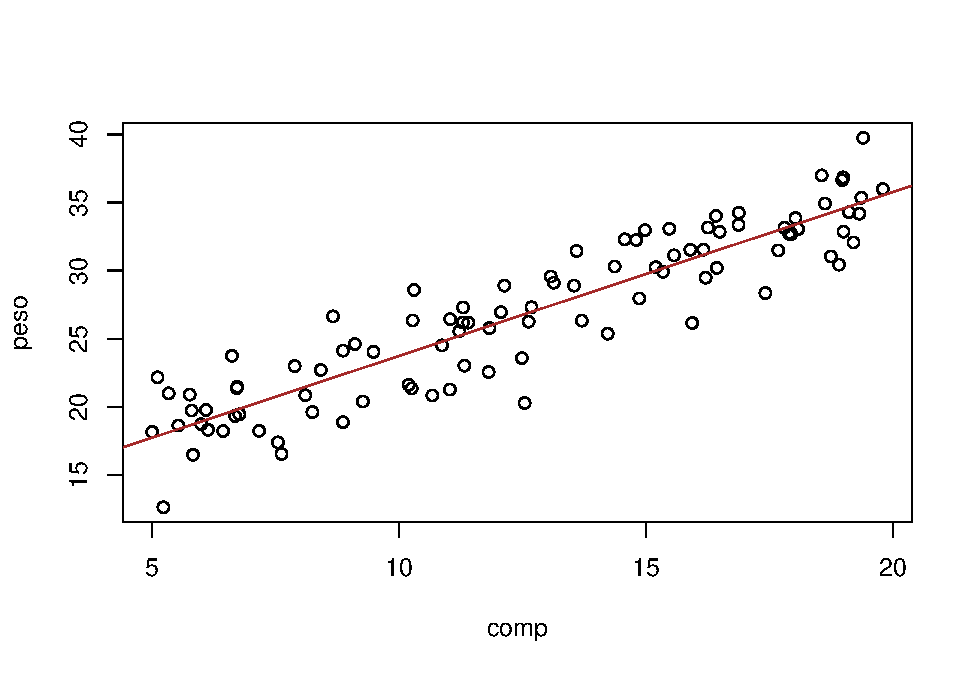
\includegraphics{ECOMODbook_files/figure-latex/a6.9-1.pdf}

Note the last line works because the parameter estimates are hold in a component of the \texttt{summary} of the fitted model called \texttt{coefficients}

\begin{Shaded}
\begin{Highlighting}[]
\FunctionTok{summary}\NormalTok{(lmlag)}\SpecialCharTok{$}\NormalTok{coefficients}
\end{Highlighting}
\end{Shaded}

\begin{verbatim}
##              Estimate Std. Error  t value     Pr(>|t|)
## (Intercept) 11.722343 0.72299153 16.21367 4.135172e-29
## comp         1.202333 0.05402397 22.25555 1.839784e-39
\end{verbatim}

Additionally, we can also add the residuals in the plot (we use the very handy function \texttt{segments}, that adds segments to plots, to do so)

\begin{Shaded}
\begin{Highlighting}[]
\CommentTok{\# get estimated/predicted values with function residuals}
\NormalTok{estimated2}\OtherTok{\textless{}{-}}\FunctionTok{predict}\NormalTok{(lmlag)}
\CommentTok{\#plot the data}
\FunctionTok{with}\NormalTok{(lagartos,}\FunctionTok{plot}\NormalTok{(peso}\SpecialCharTok{\textasciitilde{}}\NormalTok{comp,}\AttributeTok{pch=}\DecValTok{21}\NormalTok{,}\AttributeTok{bg=}\StringTok{"brown"}\NormalTok{,}\AttributeTok{col=}\StringTok{"green"}\NormalTok{))}
\FunctionTok{abline}\NormalTok{(lmlag,}\AttributeTok{col=}\DecValTok{3}\NormalTok{,}\AttributeTok{lty=}\DecValTok{2}\NormalTok{)}
\CommentTok{\#add residuals}
\FunctionTok{with}\NormalTok{(lagartos,}\FunctionTok{segments}\NormalTok{(}\AttributeTok{x0 =}\NormalTok{ comp,}\AttributeTok{y0 =}\NormalTok{ peso, }\AttributeTok{x1=}\NormalTok{ comp, }\AttributeTok{y1=}\NormalTok{estimated,}\AttributeTok{lty=}\DecValTok{2}\NormalTok{,}\AttributeTok{col=}\StringTok{"red"}\NormalTok{))}
\end{Highlighting}
\end{Shaded}

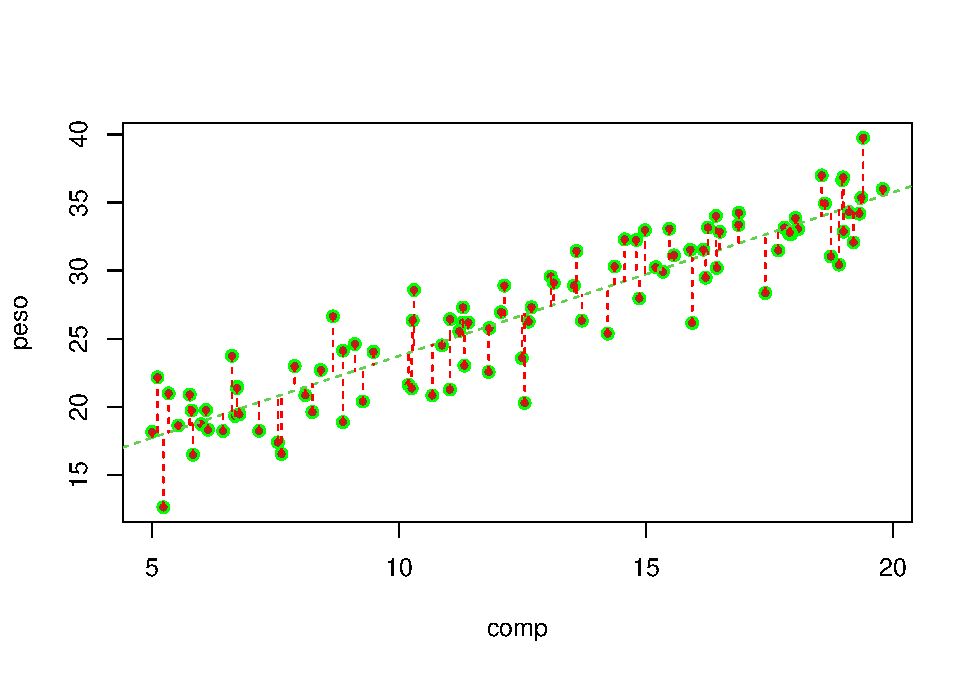
\includegraphics{ECOMODbook_files/figure-latex/a6.11-1.pdf}

The regression line is the line that minimizes the sum of the red distances in the plot above. That is also why it is called a minimum squares estimate in the special case of a Gaussian model (in PT, é a reta dos mínimos quadrados).

The residuals should, if the model is reasonable - and here that should be the case - be well approximated by a Gaussian distribution. Note we can get the values of the residuals by the difference between the observations and the estimated values, as we did above. We can look at their histogram below

\begin{Shaded}
\begin{Highlighting}[]
\FunctionTok{hist}\NormalTok{(resid,}\AttributeTok{main=}\StringTok{"Residuals by hand"}\NormalTok{,}\AttributeTok{freq=}\ConstantTok{FALSE}\NormalTok{)}
\CommentTok{\#adding the theorethical density of a Gaussian with mean 0 and the}
\CommentTok{\#correct standard error}
\FunctionTok{lines}\NormalTok{(}\FunctionTok{seq}\NormalTok{(}\SpecialCharTok{{-}}\DecValTok{8}\NormalTok{,}\DecValTok{8}\NormalTok{,}\AttributeTok{by=}\FloatTok{0.1}\NormalTok{),}\FunctionTok{dnorm}\NormalTok{(}\FunctionTok{seq}\NormalTok{(}\SpecialCharTok{{-}}\DecValTok{8}\NormalTok{,}\DecValTok{8}\NormalTok{,}\AttributeTok{by=}\FloatTok{0.1}\NormalTok{),}\AttributeTok{mean=}\DecValTok{0}\NormalTok{,}\AttributeTok{sd=}\FunctionTok{summary}\NormalTok{(lmlag)}\SpecialCharTok{$}\NormalTok{sigma))}
\end{Highlighting}
\end{Shaded}

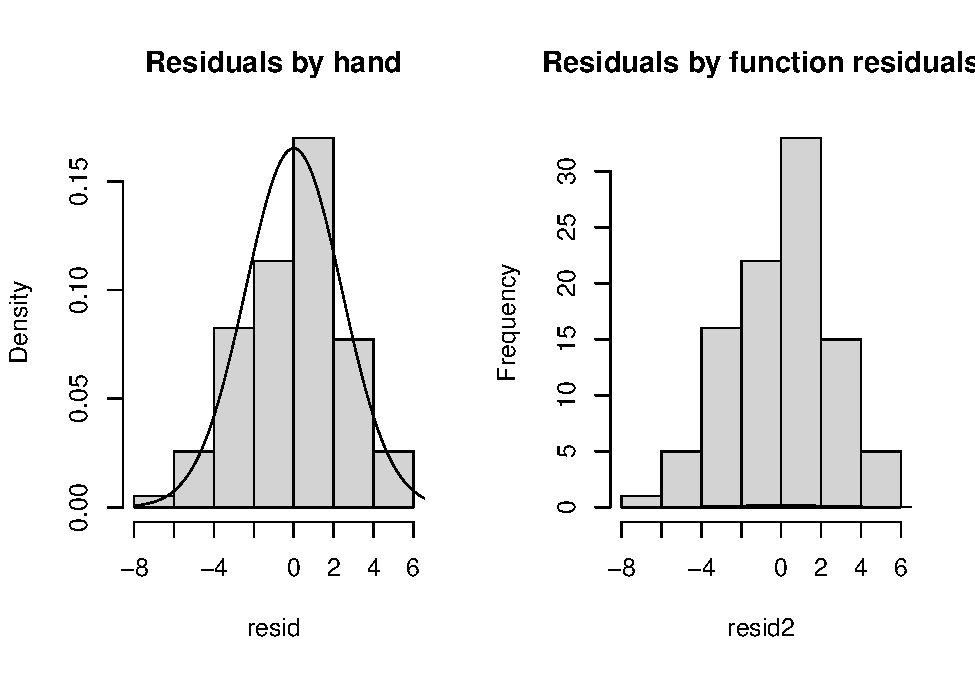
\includegraphics{ECOMODbook_files/figure-latex/a6.12-1.pdf}

or alternatively we can use the bespoke function \texttt{residuals}

\begin{Shaded}
\begin{Highlighting}[]
\NormalTok{resid2}\OtherTok{\textless{}{-}}\FunctionTok{residuals}\NormalTok{(lmlag)}
\FunctionTok{hist}\NormalTok{(resid2,}\AttributeTok{main=}\StringTok{"Residuals by function residuals"}\NormalTok{)}
\end{Highlighting}
\end{Shaded}

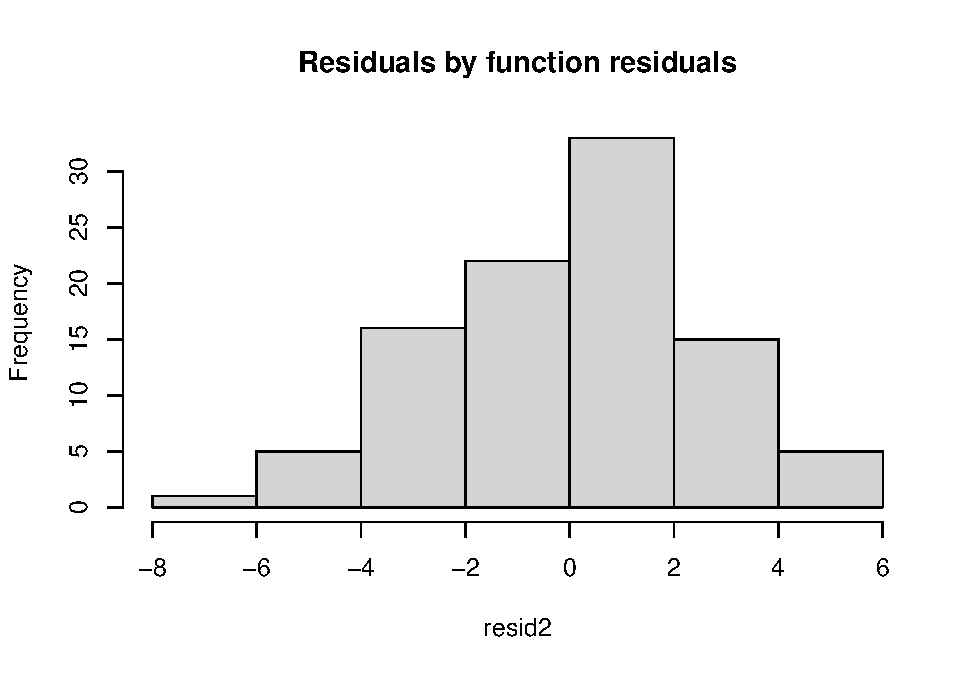
\includegraphics{ECOMODbook_files/figure-latex/a6.13-1.pdf}

It is often said that the \(R^2\) represents the amount of variation in the response that the regression explains. Why is that?

Because if you assume that all the variability in the response data, the \(y_i\) the diference between the data points and a common mean

\[\sum_{i=1}^n (y_i- \bar y)^2\]

in an image, the sum of the square of these quantities

\begin{Shaded}
\begin{Highlighting}[]
\CommentTok{\#plot}
\FunctionTok{with}\NormalTok{(lagartos,}\FunctionTok{plot}\NormalTok{(peso}\SpecialCharTok{\textasciitilde{}}\NormalTok{comp))}
\FunctionTok{abline}\NormalTok{(lmlag,}\AttributeTok{col=}\DecValTok{3}\NormalTok{,}\AttributeTok{lty=}\DecValTok{2}\NormalTok{)}
\FunctionTok{abline}\NormalTok{(}\AttributeTok{h=}\FunctionTok{mean}\NormalTok{(lagartos}\SpecialCharTok{$}\NormalTok{peso))}
\FunctionTok{with}\NormalTok{(lagartos,}\FunctionTok{segments}\NormalTok{(}\AttributeTok{x0 =}\NormalTok{ comp,}\AttributeTok{y0 =}\NormalTok{ peso, }\AttributeTok{x1=}\NormalTok{ comp, }\AttributeTok{y1=}\FunctionTok{mean}\NormalTok{(peso),}\AttributeTok{lty=}\DecValTok{2}\NormalTok{,}\AttributeTok{col=}\DecValTok{2}\NormalTok{))}
\end{Highlighting}
\end{Shaded}

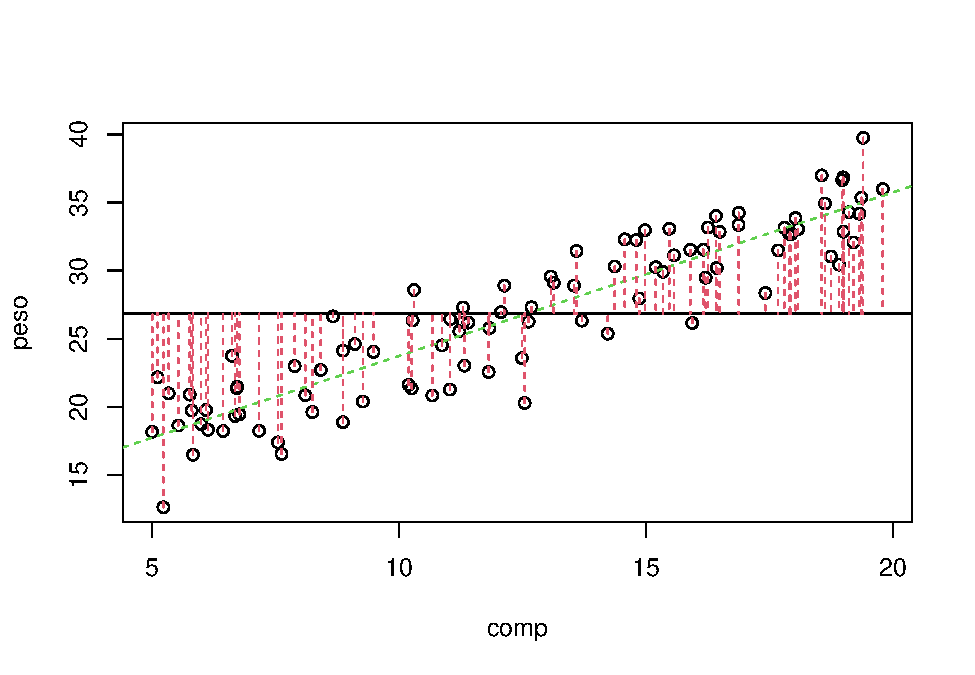
\includegraphics{ECOMODbook_files/figure-latex/a6.14-1.pdf}

\begin{Shaded}
\begin{Highlighting}[]
\NormalTok{all.var}\OtherTok{\textless{}{-}}\FunctionTok{sum}\NormalTok{((lagartos}\SpecialCharTok{$}\NormalTok{peso}\SpecialCharTok{{-}}\FunctionTok{mean}\NormalTok{(lagartos}\SpecialCharTok{$}\NormalTok{peso))}\SpecialCharTok{\^{}}\DecValTok{2}\NormalTok{)}
\NormalTok{all.var}
\end{Highlighting}
\end{Shaded}

\begin{verbatim}
## [1] 3441.795
\end{verbatim}

and the variability that is not explained is the one that remains in the errors (the corresponding plot was shown above)

\[\sum_{i=1}^n (y_i- \hat y_i)^2\]

\begin{Shaded}
\begin{Highlighting}[]
\NormalTok{error.var}\OtherTok{\textless{}{-}}\FunctionTok{sum}\NormalTok{((lagartos}\SpecialCharTok{$}\NormalTok{peso}\SpecialCharTok{{-}}\NormalTok{estimated)}\SpecialCharTok{\^{}}\DecValTok{2}\NormalTok{)}
\NormalTok{error.var}
\end{Highlighting}
\end{Shaded}

\begin{verbatim}
## [1] 553.8968
\end{verbatim}

then the ratio of those two quantities is what is NOT explained by the regression model, and therefore, 1 minus that is what explained by the regression model.

\begin{Shaded}
\begin{Highlighting}[]
\DecValTok{1}\SpecialCharTok{{-}}\NormalTok{error.var}\SpecialCharTok{/}\NormalTok{all.var}
\end{Highlighting}
\end{Shaded}

\begin{verbatim}
## [1] 0.8390675
\end{verbatim}

And that\ldots{} as noted above\ldots{} is the \(R^2\)=0.8391. This comes from the fact that all of the variability in the data (the \(y\), the response, here the \texttt{peso}) can be decomposed into the variability explained by the model, and the unexplained variability, that of the errors. In a formula

\[SS_{TOTAL}=SS_{REGRESSÃO}+SS_{ERRO}\]

Note naturally we could also represent in an image what is explained by the regression model, which is

\[\sum_{i=1}^n (\hat y_i- \bar y)^2\]

\begin{Shaded}
\begin{Highlighting}[]
\CommentTok{\#plot}
\FunctionTok{with}\NormalTok{(lagartos,}\FunctionTok{plot}\NormalTok{(peso}\SpecialCharTok{\textasciitilde{}}\NormalTok{comp))}
\FunctionTok{abline}\NormalTok{(lmlag,}\AttributeTok{col=}\DecValTok{3}\NormalTok{,}\AttributeTok{lty=}\DecValTok{2}\NormalTok{)}
\FunctionTok{abline}\NormalTok{(}\AttributeTok{h=}\FunctionTok{mean}\NormalTok{(lagartos}\SpecialCharTok{$}\NormalTok{peso))}
\FunctionTok{with}\NormalTok{(lagartos,}\FunctionTok{segments}\NormalTok{(}\AttributeTok{x0 =}\NormalTok{ comp,}\AttributeTok{y0 =}\NormalTok{ estimated, }\AttributeTok{x1=}\NormalTok{ comp, }\AttributeTok{y1=}\FunctionTok{mean}\NormalTok{(peso),}\AttributeTok{lty=}\DecValTok{2}\NormalTok{,}\AttributeTok{col=}\DecValTok{2}\NormalTok{))}
\end{Highlighting}
\end{Shaded}

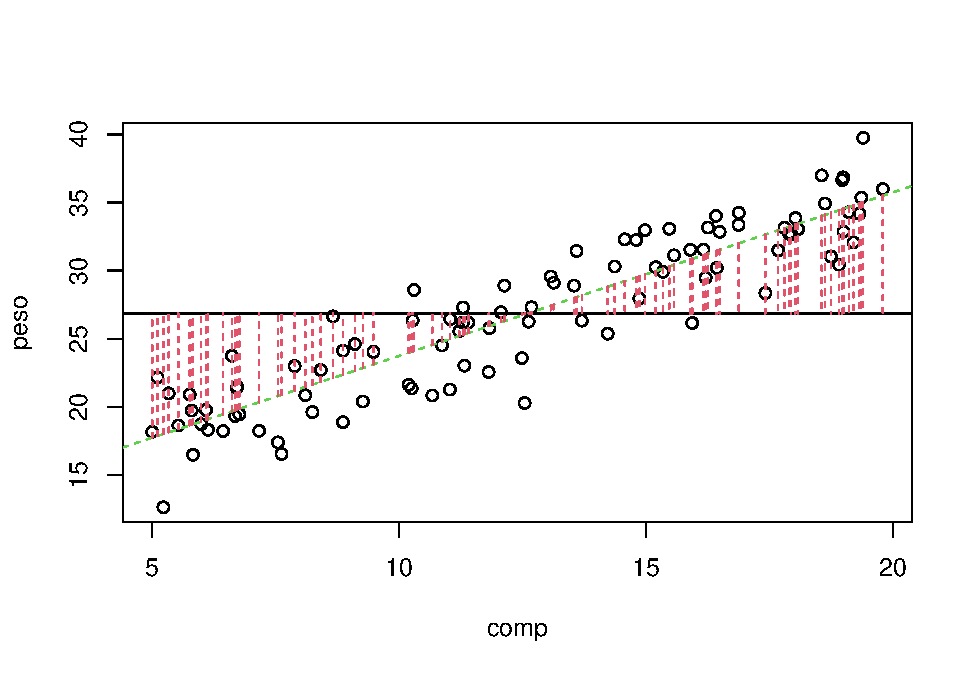
\includegraphics{ECOMODbook_files/figure-latex/a6.18-1.pdf}

and that naturally is obtained as

\begin{Shaded}
\begin{Highlighting}[]
\NormalTok{reg.var}\OtherTok{\textless{}{-}}\FunctionTok{sum}\NormalTok{((}\FunctionTok{mean}\NormalTok{(lagartos}\SpecialCharTok{$}\NormalTok{peso)}\SpecialCharTok{{-}}\NormalTok{estimated)}\SpecialCharTok{\^{}}\DecValTok{2}\NormalTok{)}
\NormalTok{reg.var}
\end{Highlighting}
\end{Shaded}

\begin{verbatim}
## [1] 2887.898
\end{verbatim}

and hence the total variability is given by the sum \(SS_{REGRESSÃO}+SS_{ERRO}\)

\begin{Shaded}
\begin{Highlighting}[]
\NormalTok{reg.var}\SpecialCharTok{+}\NormalTok{error.var}
\end{Highlighting}
\end{Shaded}

\begin{verbatim}
## [1] 3441.795
\end{verbatim}

\begin{Shaded}
\begin{Highlighting}[]
\NormalTok{all.var}
\end{Highlighting}
\end{Shaded}

\begin{verbatim}
## [1] 3441.795
\end{verbatim}

So, always remember that

\[SS_{TOTAL}=SS_{REGRESSÃO}+SS_{ERRO}\]

This is also something that comes out often in books without a clear explanation of the reaon why that holds. While here I show it by example, it could be easily demonstrated algebraically if one wanted that

\[\sum_{i=1}^n (y_i- \bar y)^2=\sum_{i=1}^n (\hat y_i- \bar y)^2 + \sum_{i=1}^n (y_i- \hat y_i)^2\]

If you want that, this 28 minute video shows you the proof: \url{https://www.youtube.com/watch?v=aQ32qTjqqJM}
I think it could take just 5 minutes ;) but many thanks to Dmitry Leiderman for having it out there! He does it in the context of ANOVA, but ANOVA is just a special case of regression, were you have a continous response and a single categorical explanatory variable. Therefore, have fun !

\hypertarget{simulating-regression-data}{%
\section{Simulating regression data}\label{simulating-regression-data}}

Using the above, simulate data assuming that the TRUE relation between the weight and length of a lizzard was given by

\[ peso = 12 + 1.2 * comp \]

We consider that the usual length of a lizard can be between 5 and 20 cm, and the standard error is 4.

As in the data we will have 97 lizards

Then you were told to create the lengths:

\begin{Shaded}
\begin{Highlighting}[]
\FunctionTok{set.seed}\NormalTok{(}\DecValTok{121}\NormalTok{)}
\NormalTok{n}\OtherTok{=}\DecValTok{97}
\CommentTok{\#lengths}
\NormalTok{xs}\OtherTok{=}\FunctionTok{runif}\NormalTok{(n,}\DecValTok{5}\NormalTok{,}\DecValTok{20}\NormalTok{)}
\FunctionTok{hist}\NormalTok{(xs,}\AttributeTok{main=}\StringTok{"Lenths (cm)"}\NormalTok{)}
\end{Highlighting}
\end{Shaded}

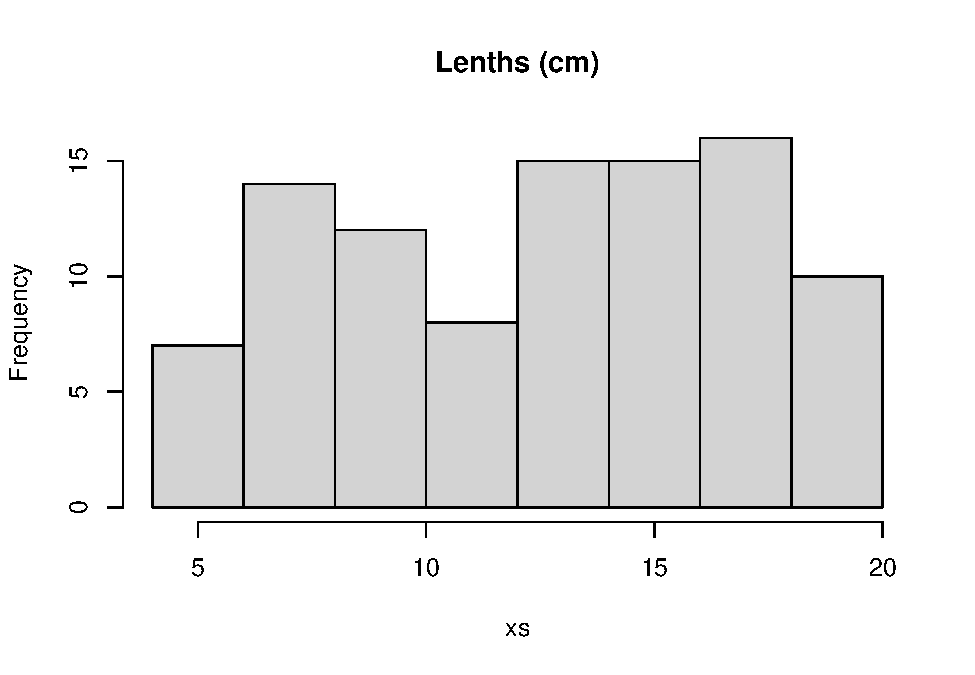
\includegraphics{ECOMODbook_files/figure-latex/a6.21-1.pdf}

and then to create weights of lizards

\begin{Shaded}
\begin{Highlighting}[]
\NormalTok{a}\OtherTok{=}\DecValTok{12}
\NormalTok{b}\OtherTok{=}\FloatTok{1.2}
\NormalTok{ys}\OtherTok{=}\NormalTok{a}\SpecialCharTok{+}\NormalTok{b}\SpecialCharTok{*}\NormalTok{xs}
\end{Highlighting}
\end{Shaded}

If we plot the data, all points are in a single line. Why, because there is no randomness.

\begin{Shaded}
\begin{Highlighting}[]
\FunctionTok{plot}\NormalTok{(xs,ys)}
\end{Highlighting}
\end{Shaded}

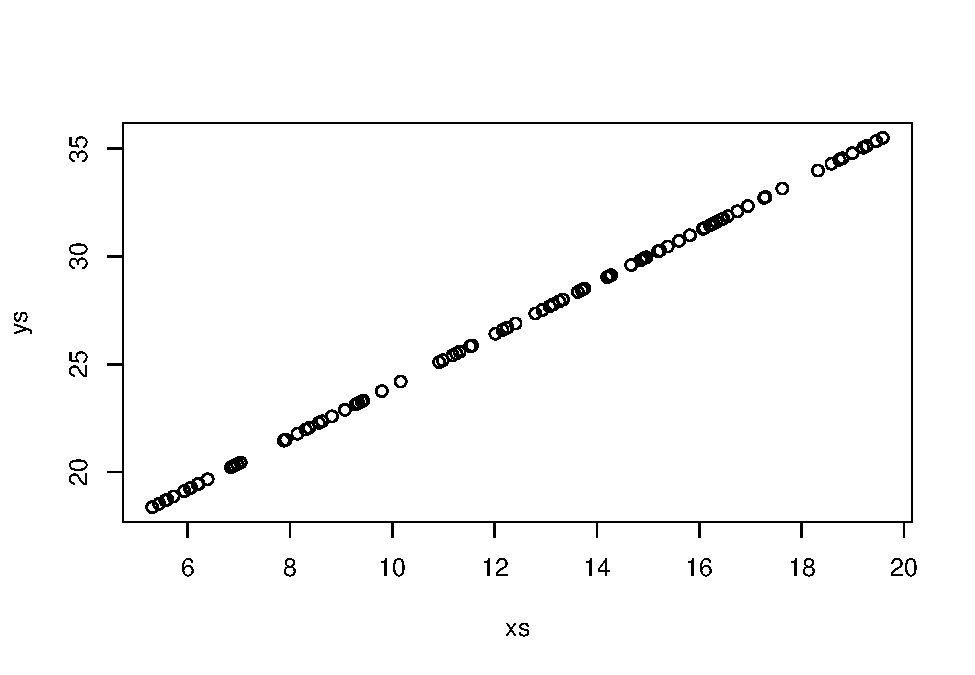
\includegraphics{ECOMODbook_files/figure-latex/a6.23-1.pdf}

This means that if you try to run a model, it gives you a warning that the model might be unreliable

\begin{Shaded}
\begin{Highlighting}[]
\FunctionTok{summary}\NormalTok{(}\FunctionTok{lm}\NormalTok{(ys}\SpecialCharTok{\textasciitilde{}}\NormalTok{xs))}
\end{Highlighting}
\end{Shaded}

\begin{verbatim}
## Warning in summary.lm(lm(ys ~ xs)): essentially perfect fit: summary may be
## unreliable
\end{verbatim}

\begin{verbatim}
## 
## Call:
## lm(formula = ys ~ xs)
## 
## Residuals:
##        Min         1Q     Median         3Q        Max 
## -5.595e-15 -2.460e-15 -1.878e-15 -1.422e-15  1.873e-13 
## 
## Coefficients:
##              Estimate Std. Error   t value Pr(>|t|)    
## (Intercept) 1.200e+01  6.050e-15 1.983e+15   <2e-16 ***
## xs          1.200e+00  4.611e-16 2.603e+15   <2e-16 ***
## ---
## Signif. codes:  0 '***' 0.001 '**' 0.01 '*' 0.05 '.' 0.1 ' ' 1
## 
## Residual standard error: 1.934e-14 on 95 degrees of freedom
## Multiple R-squared:      1,  Adjusted R-squared:      1 
## F-statistic: 6.773e+30 on 1 and 95 DF,  p-value: < 2.2e-16
\end{verbatim}

So\ldots{} , we add some variance, and plot the data:

\begin{Shaded}
\begin{Highlighting}[]
\NormalTok{ys}\OtherTok{=}\NormalTok{a}\SpecialCharTok{+}\NormalTok{b}\SpecialCharTok{*}\NormalTok{xs}\SpecialCharTok{+}\FunctionTok{rnorm}\NormalTok{(n,}\DecValTok{0}\NormalTok{,}\DecValTok{4}\NormalTok{)}
\FunctionTok{plot}\NormalTok{(xs,ys)}
\end{Highlighting}
\end{Shaded}

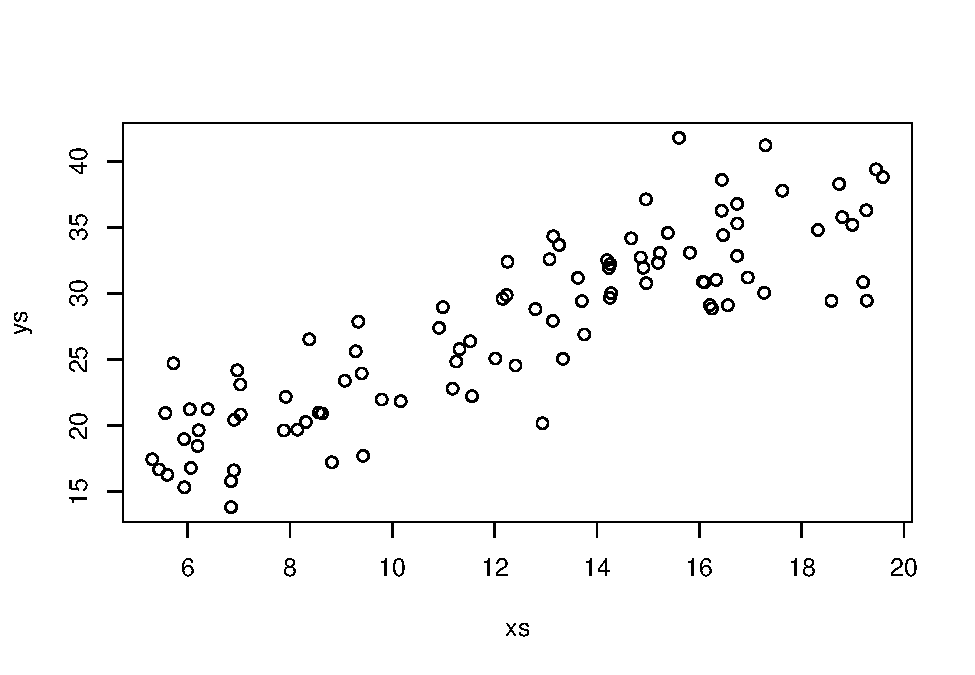
\includegraphics{ECOMODbook_files/figure-latex/a6.25-1.pdf}

Using the code above, experiment with changing the standard deviation of the error, and see what happens to the estimated \(R^2\), to the parameter estimates, to the estimated error, and to how close the estimated regression mode is to the true model (note this is the amazing advantage of a simulation, which we do not have in real data, we know what reality is, and a true model exists!). This will give you a good feeling for what a regression model is and what is does, and what it can't do. An example of what it can't give you is reliable estimates when the error is large compared to the systematic part of the model.

\begin{Shaded}
\begin{Highlighting}[]
\NormalTok{n }\OtherTok{\textless{}{-}} \DecValTok{97}
\CommentTok{\#simular comprimentos}
\NormalTok{comp.sim }\OtherTok{\textless{}{-}} \FunctionTok{runif}\NormalTok{(n,}\DecValTok{5}\NormalTok{,}\DecValTok{20}\NormalTok{)}
\NormalTok{a}\OtherTok{\textless{}{-}}\DecValTok{12}
\NormalTok{b}\OtherTok{\textless{}{-}}\FloatTok{1.2}
\CommentTok{\#simular pesos}
\NormalTok{peso.sim}\OtherTok{\textless{}{-}}\NormalTok{a}\SpecialCharTok{+}\NormalTok{b}\SpecialCharTok{*}\NormalTok{comp.sim}\SpecialCharTok{+}\FunctionTok{rnorm}\NormalTok{(n,}\AttributeTok{mean=}\DecValTok{0}\NormalTok{,}\AttributeTok{sd=}\DecValTok{2}\NormalTok{)}
\NormalTok{data.sim}\OtherTok{=}\FunctionTok{data.frame}\NormalTok{(}\AttributeTok{csim=}\NormalTok{comp.sim,}\AttributeTok{psim=}\NormalTok{peso.sim)}
\FunctionTok{plot}\NormalTok{(psim}\SpecialCharTok{\textasciitilde{}}\NormalTok{csim,}\AttributeTok{data=}\NormalTok{data.sim)}
\NormalTok{mod.sim}\OtherTok{\textless{}{-}}\FunctionTok{lm}\NormalTok{(psim}\SpecialCharTok{\textasciitilde{}}\NormalTok{csim,}\AttributeTok{data=}\NormalTok{data.sim)}
\FunctionTok{abline}\NormalTok{(mod.sim,}\AttributeTok{col=}\StringTok{"red"}\NormalTok{)}
\FunctionTok{summary}\NormalTok{(mod.sim)}
\end{Highlighting}
\end{Shaded}

\begin{verbatim}
## 
## Call:
## lm(formula = psim ~ csim, data = data.sim)
## 
## Residuals:
##     Min      1Q  Median      3Q     Max 
## -5.3460 -1.1652  0.1329  1.5072  3.0036 
## 
## Coefficients:
##             Estimate Std. Error t value Pr(>|t|)    
## (Intercept) 11.70390    0.56783   20.61   <2e-16 ***
## csim         1.20912    0.04325   27.96   <2e-16 ***
## ---
## Signif. codes:  0 '***' 0.001 '**' 0.01 '*' 0.05 '.' 0.1 ' ' 1
## 
## Residual standard error: 1.822 on 95 degrees of freedom
## Multiple R-squared:  0.8916, Adjusted R-squared:  0.8905 
## F-statistic: 781.6 on 1 and 95 DF,  p-value: < 2.2e-16
\end{verbatim}

\begin{Shaded}
\begin{Highlighting}[]
\FunctionTok{abline}\NormalTok{(a,b,}\AttributeTok{col=}\StringTok{"green"}\NormalTok{)}
\FunctionTok{legend}\NormalTok{(}\StringTok{"topleft"}\NormalTok{,}\AttributeTok{legend=}\FunctionTok{c}\NormalTok{(}\StringTok{"Estimated line"}\NormalTok{,}\StringTok{"True model"}\NormalTok{),}\AttributeTok{col=}\FunctionTok{c}\NormalTok{(}\StringTok{"red"}\NormalTok{,}\StringTok{"green"}\NormalTok{),}\AttributeTok{lty=}\DecValTok{1}\NormalTok{,}\AttributeTok{inset=}\FloatTok{0.05}\NormalTok{)}
\end{Highlighting}
\end{Shaded}

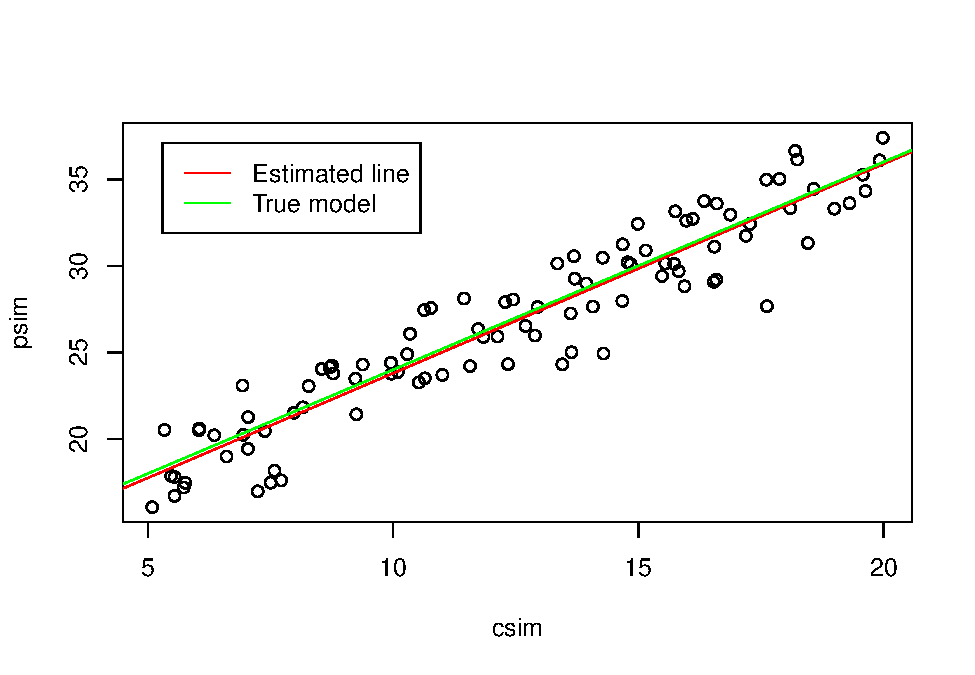
\includegraphics{ECOMODbook_files/figure-latex/a6.26-1.pdf}

\hypertarget{what-is-the-effect-of-increasing-the-error-a-simulation-experiment}{%
\subsection{What is the effect of increasing the error: a simulation experiment}\label{what-is-the-effect-of-increasing-the-error-a-simulation-experiment}}

Now, let's consider there's more and less variance. We also add to each plot the real line (that with the true parameter values) and the one with the estimated parameter values.

\begin{Shaded}
\begin{Highlighting}[]
\FunctionTok{par}\NormalTok{(}\AttributeTok{mfrow=}\FunctionTok{c}\NormalTok{(}\DecValTok{2}\NormalTok{,}\DecValTok{3}\NormalTok{))}
\NormalTok{ys}\OtherTok{=}\NormalTok{a}\SpecialCharTok{+}\NormalTok{b}\SpecialCharTok{*}\NormalTok{xs}\SpecialCharTok{+}\FunctionTok{rnorm}\NormalTok{(n,}\DecValTok{0}\NormalTok{,}\DecValTok{1}\NormalTok{)}
\FunctionTok{plot}\NormalTok{(xs,ys)}
\NormalTok{mod1}\OtherTok{=}\FunctionTok{lm}\NormalTok{(ys}\SpecialCharTok{\textasciitilde{}}\NormalTok{xs)}
\FunctionTok{abline}\NormalTok{(mod1,}\AttributeTok{col=}\StringTok{"red"}\NormalTok{)}
\FunctionTok{abline}\NormalTok{(a,b,}\AttributeTok{col=}\StringTok{"green"}\NormalTok{)}
\NormalTok{ys}\OtherTok{=}\NormalTok{a}\SpecialCharTok{+}\NormalTok{b}\SpecialCharTok{*}\NormalTok{xs}\SpecialCharTok{+}\FunctionTok{rnorm}\NormalTok{(n,}\DecValTok{0}\NormalTok{,}\DecValTok{2}\NormalTok{)}
\FunctionTok{plot}\NormalTok{(xs,ys)}
\NormalTok{mod2}\OtherTok{=}\FunctionTok{lm}\NormalTok{(ys}\SpecialCharTok{\textasciitilde{}}\NormalTok{xs)}
\FunctionTok{abline}\NormalTok{(mod2,}\AttributeTok{col=}\StringTok{"red"}\NormalTok{)}
\FunctionTok{abline}\NormalTok{(a,b,}\AttributeTok{col=}\StringTok{"green"}\NormalTok{)}
\NormalTok{ys}\OtherTok{=}\NormalTok{a}\SpecialCharTok{+}\NormalTok{b}\SpecialCharTok{*}\NormalTok{xs}\SpecialCharTok{+}\FunctionTok{rnorm}\NormalTok{(n,}\DecValTok{0}\NormalTok{,}\DecValTok{4}\NormalTok{)}
\FunctionTok{plot}\NormalTok{(xs,ys)}
\NormalTok{mod4}\OtherTok{=}\FunctionTok{lm}\NormalTok{(ys}\SpecialCharTok{\textasciitilde{}}\NormalTok{xs)}
\FunctionTok{abline}\NormalTok{(mod4,}\AttributeTok{col=}\StringTok{"red"}\NormalTok{)}
\FunctionTok{abline}\NormalTok{(a,b,}\AttributeTok{col=}\StringTok{"green"}\NormalTok{)}
\NormalTok{ys}\OtherTok{=}\NormalTok{a}\SpecialCharTok{+}\NormalTok{b}\SpecialCharTok{*}\NormalTok{xs}\SpecialCharTok{+}\FunctionTok{rnorm}\NormalTok{(n,}\DecValTok{0}\NormalTok{,}\DecValTok{10}\NormalTok{)}
\FunctionTok{plot}\NormalTok{(xs,ys)}
\NormalTok{mod10}\OtherTok{=}\FunctionTok{lm}\NormalTok{(ys}\SpecialCharTok{\textasciitilde{}}\NormalTok{xs)}
\FunctionTok{abline}\NormalTok{(mod10,}\AttributeTok{col=}\StringTok{"red"}\NormalTok{)}
\FunctionTok{abline}\NormalTok{(a,b,}\AttributeTok{col=}\StringTok{"green"}\NormalTok{)}
\NormalTok{ys}\OtherTok{=}\NormalTok{a}\SpecialCharTok{+}\NormalTok{b}\SpecialCharTok{*}\NormalTok{xs}\SpecialCharTok{+}\FunctionTok{rnorm}\NormalTok{(n,}\DecValTok{0}\NormalTok{,}\DecValTok{20}\NormalTok{)}
\FunctionTok{plot}\NormalTok{(xs,ys)}
\NormalTok{mod20}\OtherTok{=}\FunctionTok{lm}\NormalTok{(ys}\SpecialCharTok{\textasciitilde{}}\NormalTok{xs)}
\FunctionTok{abline}\NormalTok{(mod20,}\AttributeTok{col=}\StringTok{"red"}\NormalTok{)}
\FunctionTok{abline}\NormalTok{(a,b,}\AttributeTok{col=}\StringTok{"green"}\NormalTok{)}
\NormalTok{ys}\OtherTok{=}\NormalTok{a}\SpecialCharTok{+}\NormalTok{b}\SpecialCharTok{*}\NormalTok{xs}\SpecialCharTok{+}\FunctionTok{rnorm}\NormalTok{(n,}\DecValTok{0}\NormalTok{,}\DecValTok{100}\NormalTok{)}
\FunctionTok{plot}\NormalTok{(xs,ys)}
\NormalTok{mod100}\OtherTok{=}\FunctionTok{lm}\NormalTok{(ys}\SpecialCharTok{\textasciitilde{}}\NormalTok{xs)}
\FunctionTok{abline}\NormalTok{(mod100,}\AttributeTok{col=}\StringTok{"red"}\NormalTok{)}
\FunctionTok{abline}\NormalTok{(a,b,}\AttributeTok{col=}\StringTok{"green"}\NormalTok{)}
\end{Highlighting}
\end{Shaded}

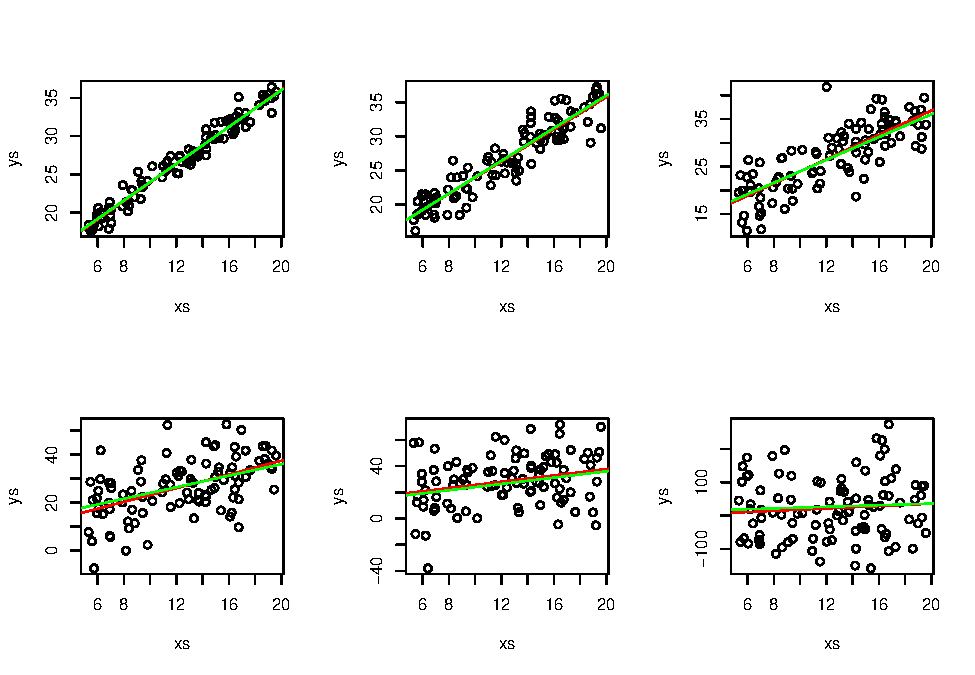
\includegraphics{ECOMODbook_files/figure-latex/a6.27-1.pdf}

Not surprisingly, as the variance increases, we get data that more and more looks like it is not coming from a real linear process.

You can also look at the model summaries, and there you can see that, in fact, the models become essentially useless as the variance increases! You can see that both from the correlation, but also by the predictions generated from the model (comparing to the truth), and also the significance of the coefficients associated with the regression parameters.

Make no mistake, the reality is always the same, in terms of the fixed part of the model, it's just the variance that increases.

Also, don't get confused, the different green lines might look different, but they are always exactly the same line! You can check that by forcing the y axis to span the same limits.

\begin{Shaded}
\begin{Highlighting}[]
\FunctionTok{par}\NormalTok{(}\AttributeTok{mfrow=}\FunctionTok{c}\NormalTok{(}\DecValTok{2}\NormalTok{,}\DecValTok{3}\NormalTok{))}
\NormalTok{ys}\OtherTok{=}\NormalTok{a}\SpecialCharTok{+}\NormalTok{b}\SpecialCharTok{*}\NormalTok{xs}\SpecialCharTok{+}\FunctionTok{rnorm}\NormalTok{(n,}\DecValTok{0}\NormalTok{,}\DecValTok{1}\NormalTok{)}
\FunctionTok{plot}\NormalTok{(xs,ys,}\AttributeTok{ylim=}\FunctionTok{c}\NormalTok{(}\SpecialCharTok{{-}}\DecValTok{400}\NormalTok{,}\DecValTok{400}\NormalTok{))}
\NormalTok{mod1}\OtherTok{=}\FunctionTok{lm}\NormalTok{(ys}\SpecialCharTok{\textasciitilde{}}\NormalTok{xs)}
\FunctionTok{abline}\NormalTok{(mod1,}\AttributeTok{col=}\StringTok{"red"}\NormalTok{)}
\FunctionTok{abline}\NormalTok{(a,b,}\AttributeTok{col=}\StringTok{"green"}\NormalTok{)}
\NormalTok{ys}\OtherTok{=}\NormalTok{a}\SpecialCharTok{+}\NormalTok{b}\SpecialCharTok{*}\NormalTok{xs}\SpecialCharTok{+}\FunctionTok{rnorm}\NormalTok{(n,}\DecValTok{0}\NormalTok{,}\DecValTok{2}\NormalTok{)}
\FunctionTok{plot}\NormalTok{(xs,ys,}\AttributeTok{ylim=}\FunctionTok{c}\NormalTok{(}\SpecialCharTok{{-}}\DecValTok{400}\NormalTok{,}\DecValTok{400}\NormalTok{))}
\NormalTok{mod2}\OtherTok{=}\FunctionTok{lm}\NormalTok{(ys}\SpecialCharTok{\textasciitilde{}}\NormalTok{xs)}
\FunctionTok{abline}\NormalTok{(mod2,}\AttributeTok{col=}\StringTok{"red"}\NormalTok{)}
\FunctionTok{abline}\NormalTok{(a,b,}\AttributeTok{col=}\StringTok{"green"}\NormalTok{)}
\NormalTok{ys}\OtherTok{=}\NormalTok{a}\SpecialCharTok{+}\NormalTok{b}\SpecialCharTok{*}\NormalTok{xs}\SpecialCharTok{+}\FunctionTok{rnorm}\NormalTok{(n,}\DecValTok{0}\NormalTok{,}\DecValTok{4}\NormalTok{)}
\FunctionTok{plot}\NormalTok{(xs,ys,}\AttributeTok{ylim=}\FunctionTok{c}\NormalTok{(}\SpecialCharTok{{-}}\DecValTok{400}\NormalTok{,}\DecValTok{400}\NormalTok{))}
\NormalTok{mod4}\OtherTok{=}\FunctionTok{lm}\NormalTok{(ys}\SpecialCharTok{\textasciitilde{}}\NormalTok{xs)}
\FunctionTok{abline}\NormalTok{(mod4,}\AttributeTok{col=}\StringTok{"red"}\NormalTok{)}
\FunctionTok{abline}\NormalTok{(a,b,}\AttributeTok{col=}\StringTok{"green"}\NormalTok{)}
\NormalTok{ys}\OtherTok{=}\NormalTok{a}\SpecialCharTok{+}\NormalTok{b}\SpecialCharTok{*}\NormalTok{xs}\SpecialCharTok{+}\FunctionTok{rnorm}\NormalTok{(n,}\DecValTok{0}\NormalTok{,}\DecValTok{10}\NormalTok{)}
\FunctionTok{plot}\NormalTok{(xs,ys,}\AttributeTok{ylim=}\FunctionTok{c}\NormalTok{(}\SpecialCharTok{{-}}\DecValTok{400}\NormalTok{,}\DecValTok{400}\NormalTok{))}
\NormalTok{mod10}\OtherTok{=}\FunctionTok{lm}\NormalTok{(ys}\SpecialCharTok{\textasciitilde{}}\NormalTok{xs)}
\FunctionTok{abline}\NormalTok{(mod10,}\AttributeTok{col=}\StringTok{"red"}\NormalTok{)}
\FunctionTok{abline}\NormalTok{(a,b,}\AttributeTok{col=}\StringTok{"green"}\NormalTok{)}
\NormalTok{ys}\OtherTok{=}\NormalTok{a}\SpecialCharTok{+}\NormalTok{b}\SpecialCharTok{*}\NormalTok{xs}\SpecialCharTok{+}\FunctionTok{rnorm}\NormalTok{(n,}\DecValTok{0}\NormalTok{,}\DecValTok{20}\NormalTok{)}
\FunctionTok{plot}\NormalTok{(xs,ys,}\AttributeTok{ylim=}\FunctionTok{c}\NormalTok{(}\SpecialCharTok{{-}}\DecValTok{400}\NormalTok{,}\DecValTok{400}\NormalTok{))}
\NormalTok{mod20}\OtherTok{=}\FunctionTok{lm}\NormalTok{(ys}\SpecialCharTok{\textasciitilde{}}\NormalTok{xs)}
\FunctionTok{abline}\NormalTok{(mod20,}\AttributeTok{col=}\StringTok{"red"}\NormalTok{)}
\FunctionTok{abline}\NormalTok{(a,b,}\AttributeTok{col=}\StringTok{"green"}\NormalTok{)}
\NormalTok{ys}\OtherTok{=}\NormalTok{a}\SpecialCharTok{+}\NormalTok{b}\SpecialCharTok{*}\NormalTok{xs}\SpecialCharTok{+}\FunctionTok{rnorm}\NormalTok{(n,}\DecValTok{0}\NormalTok{,}\DecValTok{100}\NormalTok{)}
\FunctionTok{plot}\NormalTok{(xs,ys,}\AttributeTok{ylim=}\FunctionTok{c}\NormalTok{(}\SpecialCharTok{{-}}\DecValTok{400}\NormalTok{,}\DecValTok{400}\NormalTok{))}
\NormalTok{mod100}\OtherTok{=}\FunctionTok{lm}\NormalTok{(ys}\SpecialCharTok{\textasciitilde{}}\NormalTok{xs)}
\FunctionTok{abline}\NormalTok{(mod100,}\AttributeTok{col=}\StringTok{"red"}\NormalTok{)}
\FunctionTok{abline}\NormalTok{(a,b,}\AttributeTok{col=}\StringTok{"green"}\NormalTok{)}
\end{Highlighting}
\end{Shaded}

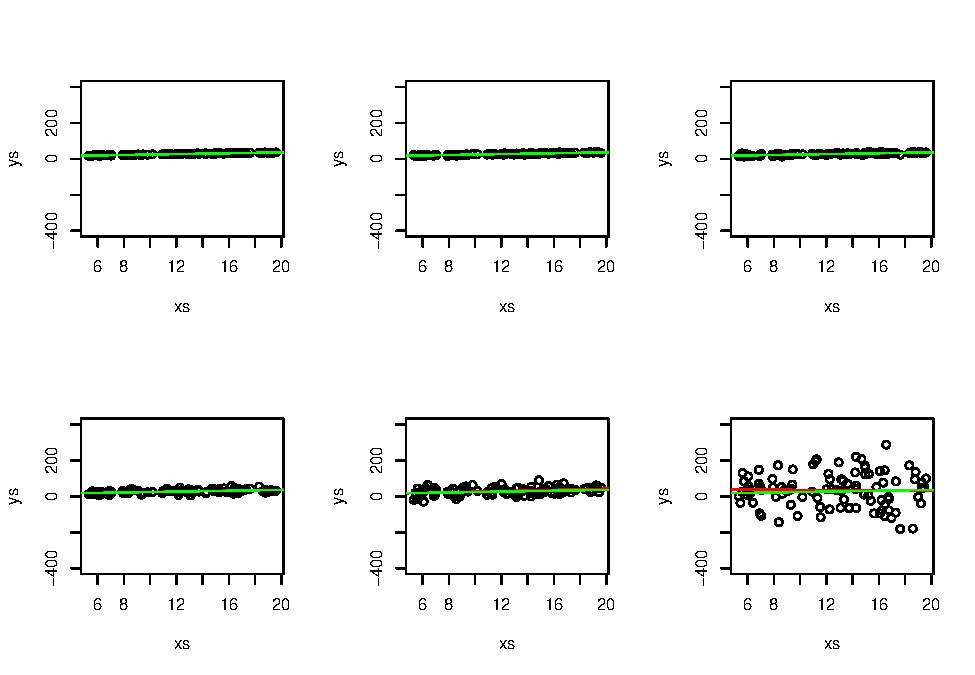
\includegraphics{ECOMODbook_files/figure-latex/a6.28-1.pdf}

but since then you loose all the ability to look at the actual data in some of the plots, that is not really that useful!

Below I look at the summary of each model. Look at correlations, at the estimated values for the parameters, their corresponding variances and the \(R^2\).

\begin{Shaded}
\begin{Highlighting}[]
\FunctionTok{summary}\NormalTok{(mod1)}
\end{Highlighting}
\end{Shaded}

\begin{verbatim}
## 
## Call:
## lm(formula = ys ~ xs)
## 
## Residuals:
##      Min       1Q   Median       3Q      Max 
## -2.87715 -0.62444  0.03329  0.69103  2.47244 
## 
## Coefficients:
##             Estimate Std. Error t value Pr(>|t|)    
## (Intercept) 12.24930    0.33691   36.36   <2e-16 ***
## xs           1.18596    0.02568   46.19   <2e-16 ***
## ---
## Signif. codes:  0 '***' 0.001 '**' 0.01 '*' 0.05 '.' 0.1 ' ' 1
## 
## Residual standard error: 1.077 on 95 degrees of freedom
## Multiple R-squared:  0.9574, Adjusted R-squared:  0.9569 
## F-statistic:  2133 on 1 and 95 DF,  p-value: < 2.2e-16
\end{verbatim}

\begin{Shaded}
\begin{Highlighting}[]
\FunctionTok{summary}\NormalTok{(mod2)}
\end{Highlighting}
\end{Shaded}

\begin{verbatim}
## 
## Call:
## lm(formula = ys ~ xs)
## 
## Residuals:
##     Min      1Q  Median      3Q     Max 
## -4.7122 -1.5245 -0.0731  1.5830  4.5457 
## 
## Coefficients:
##             Estimate Std. Error t value Pr(>|t|)    
## (Intercept) 11.22718    0.66606   16.86   <2e-16 ***
## xs           1.26028    0.05076   24.83   <2e-16 ***
## ---
## Signif. codes:  0 '***' 0.001 '**' 0.01 '*' 0.05 '.' 0.1 ' ' 1
## 
## Residual standard error: 2.129 on 95 degrees of freedom
## Multiple R-squared:  0.8665, Adjusted R-squared:  0.8651 
## F-statistic: 616.4 on 1 and 95 DF,  p-value: < 2.2e-16
\end{verbatim}

\begin{Shaded}
\begin{Highlighting}[]
\FunctionTok{summary}\NormalTok{(mod4)}
\end{Highlighting}
\end{Shaded}

\begin{verbatim}
## 
## Call:
## lm(formula = ys ~ xs)
## 
## Residuals:
##     Min      1Q  Median      3Q     Max 
## -9.8201 -2.6923  0.0809  2.8841 11.1413 
## 
## Coefficients:
##             Estimate Std. Error t value Pr(>|t|)    
## (Intercept) 12.93903    1.26042   10.27   <2e-16 ***
## xs           1.11757    0.09606   11.63   <2e-16 ***
## ---
## Signif. codes:  0 '***' 0.001 '**' 0.01 '*' 0.05 '.' 0.1 ' ' 1
## 
## Residual standard error: 4.028 on 95 degrees of freedom
## Multiple R-squared:  0.5876, Adjusted R-squared:  0.5833 
## F-statistic: 135.4 on 1 and 95 DF,  p-value: < 2.2e-16
\end{verbatim}

\begin{Shaded}
\begin{Highlighting}[]
\FunctionTok{summary}\NormalTok{(mod10)}
\end{Highlighting}
\end{Shaded}

\begin{verbatim}
## 
## Call:
## lm(formula = ys ~ xs)
## 
## Residuals:
##     Min      1Q  Median      3Q     Max 
## -23.236  -6.053  -2.186   7.375  25.314 
## 
## Coefficients:
##             Estimate Std. Error t value Pr(>|t|)    
## (Intercept)  12.1949     3.0136   4.047 0.000106 ***
## xs            1.2102     0.2297   5.269 8.54e-07 ***
## ---
## Signif. codes:  0 '***' 0.001 '**' 0.01 '*' 0.05 '.' 0.1 ' ' 1
## 
## Residual standard error: 9.632 on 95 degrees of freedom
## Multiple R-squared:  0.2262, Adjusted R-squared:  0.218 
## F-statistic: 27.76 on 1 and 95 DF,  p-value: 8.541e-07
\end{verbatim}

\begin{Shaded}
\begin{Highlighting}[]
\FunctionTok{summary}\NormalTok{(mod20)}
\end{Highlighting}
\end{Shaded}

\begin{verbatim}
## 
## Call:
## lm(formula = ys ~ xs)
## 
## Residuals:
##     Min      1Q  Median      3Q     Max 
## -48.932 -16.093   1.632  13.610  55.287 
## 
## Coefficients:
##             Estimate Std. Error t value Pr(>|t|)    
## (Intercept)   9.2412     6.4002   1.444 0.152058    
## xs            1.6652     0.4878   3.414 0.000943 ***
## ---
## Signif. codes:  0 '***' 0.001 '**' 0.01 '*' 0.05 '.' 0.1 ' ' 1
## 
## Residual standard error: 20.46 on 95 degrees of freedom
## Multiple R-squared:  0.1093, Adjusted R-squared:  0.09991 
## F-statistic: 11.66 on 1 and 95 DF,  p-value: 0.0009426
\end{verbatim}

\begin{Shaded}
\begin{Highlighting}[]
\FunctionTok{summary}\NormalTok{(mod100)}
\end{Highlighting}
\end{Shaded}

\begin{verbatim}
## 
## Call:
## lm(formula = ys ~ xs)
## 
## Residuals:
##      Min       1Q   Median       3Q      Max 
## -214.028  -69.887    0.743   60.602  255.109 
## 
## Coefficients:
##             Estimate Std. Error t value Pr(>|t|)
## (Intercept)  41.6496    30.0996   1.384    0.170
## xs           -0.5455     2.2939  -0.238    0.813
## 
## Residual standard error: 96.2 on 95 degrees of freedom
## Multiple R-squared:  0.0005949,  Adjusted R-squared:  -0.009925 
## F-statistic: 0.05655 on 1 and 95 DF,  p-value: 0.8126
\end{verbatim}

As an example, we can plot the \(R^2\) as a function of the variance

\begin{Shaded}
\begin{Highlighting}[]
\FunctionTok{plot}\NormalTok{(}\FunctionTok{c}\NormalTok{(}\DecValTok{1}\NormalTok{,}\DecValTok{2}\NormalTok{,}\DecValTok{4}\NormalTok{,}\DecValTok{10}\NormalTok{,}\DecValTok{20}\NormalTok{,}\DecValTok{100}\NormalTok{),}\FunctionTok{c}\NormalTok{(}\FunctionTok{summary}\NormalTok{(mod1)}\SpecialCharTok{$}\NormalTok{r.squared,}\FunctionTok{summary}\NormalTok{(mod2)}\SpecialCharTok{$}\NormalTok{r.squared,}\FunctionTok{summary}\NormalTok{(mod4)}\SpecialCharTok{$}\NormalTok{r.squared,}\FunctionTok{summary}\NormalTok{(mod10)}\SpecialCharTok{$}\NormalTok{r.squared,}\FunctionTok{summary}\NormalTok{(mod20)}\SpecialCharTok{$}\NormalTok{r.squared,}\FunctionTok{summary}\NormalTok{(mod100)}\SpecialCharTok{$}\NormalTok{r.squared))}
\end{Highlighting}
\end{Shaded}

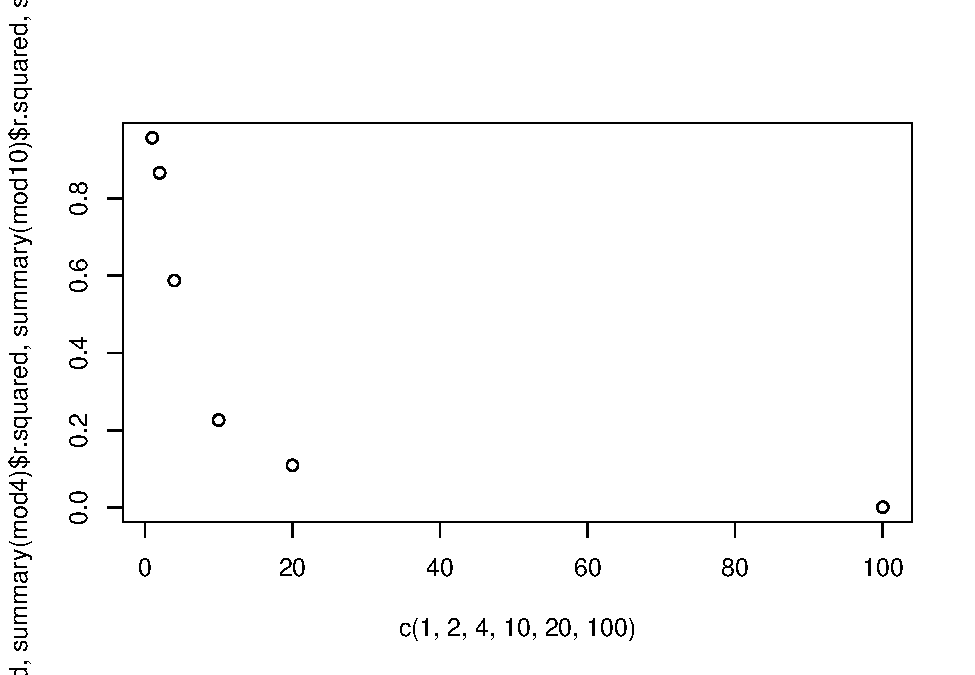
\includegraphics{ECOMODbook_files/figure-latex/a6.30-1.pdf}

That is quite interesting actually\ldots{} There seems to be a nonlinear relationship, but we only have a sample size of six (different standard deviatios, i.e., variances, as variance is standard deviation squared), so hard to tell\ldots{}

Let's show off in R\ldots{}

\begin{Shaded}
\begin{Highlighting}[]
\NormalTok{sds}\OtherTok{=}\FunctionTok{seq}\NormalTok{(}\FloatTok{0.5}\NormalTok{,}\DecValTok{100}\NormalTok{,}\AttributeTok{by=}\FloatTok{0.5}\NormalTok{)}
\NormalTok{nsds}\OtherTok{=}\FunctionTok{length}\NormalTok{(sds)}
\CommentTok{\#an object to hold the correlations}
\NormalTok{Rsqs}\OtherTok{=}\FunctionTok{numeric}\NormalTok{(nsds)}
\ControlFlowTok{for}\NormalTok{ (i }\ControlFlowTok{in} \DecValTok{1}\SpecialCharTok{:}\NormalTok{nsds)\{}
  \CommentTok{\#create data}
\NormalTok{  ys}\OtherTok{=}\NormalTok{a}\SpecialCharTok{+}\NormalTok{b}\SpecialCharTok{*}\NormalTok{xs}\SpecialCharTok{+}\FunctionTok{rnorm}\NormalTok{(n,}\DecValTok{0}\NormalTok{,sds[i])}
  \CommentTok{\#estimate model}
\NormalTok{  modi}\OtherTok{=}\FunctionTok{lm}\NormalTok{(ys}\SpecialCharTok{\textasciitilde{}}\NormalTok{xs)}
  \CommentTok{\#get R{-}squared}
\NormalTok{  Rsqs[i]}\OtherTok{=}\FunctionTok{summary}\NormalTok{(modi)}\SpecialCharTok{$}\NormalTok{r.squared}
\NormalTok{\}}
\CommentTok{\#and at the end... plot results}
\FunctionTok{plot}\NormalTok{(sds,Rsqs)}
\end{Highlighting}
\end{Shaded}

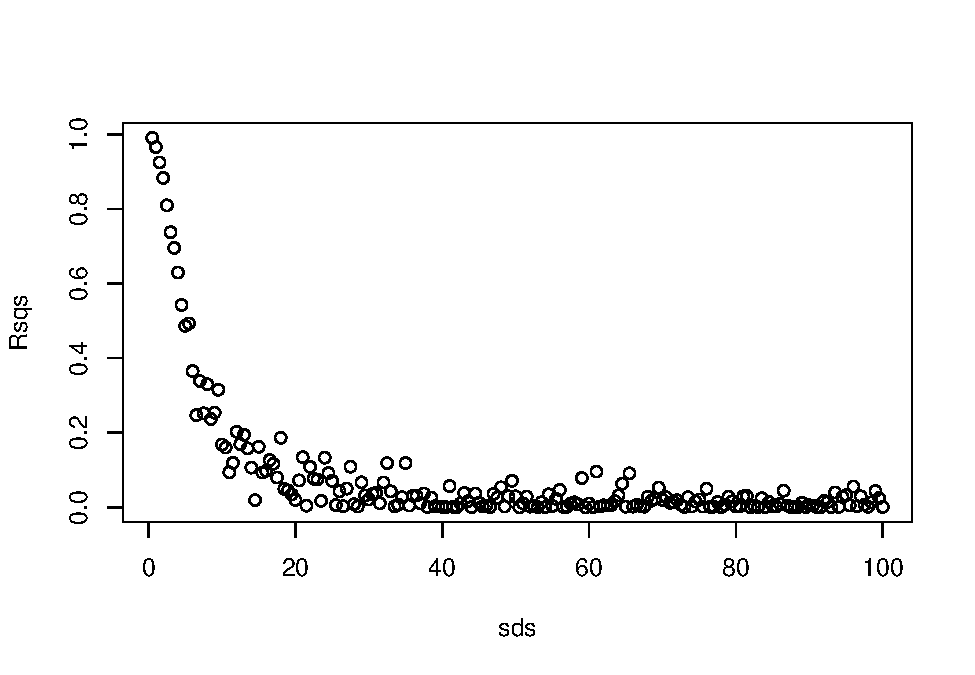
\includegraphics{ECOMODbook_files/figure-latex/a6.31-1.pdf}

How cool is that!! Actually, this means we can model the \(R^2\) as a function of the original variance! But we would not be able to model it using a linear model\ldots{}

You are not supposed to know about this yet, but I'll continue to show off. Let's use a GAM

\begin{Shaded}
\begin{Highlighting}[]
\FunctionTok{library}\NormalTok{(mgcv)}
\end{Highlighting}
\end{Shaded}

\begin{verbatim}
## Loading required package: nlme
\end{verbatim}

\begin{verbatim}
## This is mgcv 1.8-34. For overview type 'help("mgcv-package")'.
\end{verbatim}

\begin{Shaded}
\begin{Highlighting}[]
\NormalTok{gam1}\OtherTok{=}\FunctionTok{gam}\NormalTok{(Rsqs}\SpecialCharTok{\textasciitilde{}}\FunctionTok{s}\NormalTok{(sds),}\AttributeTok{link=}\NormalTok{log)}
\CommentTok{\#make predictions to plot the estimated GAM model}
\NormalTok{predRsqs}\OtherTok{=}\FunctionTok{predict.gam}\NormalTok{(gam1,}\AttributeTok{newdata =} \FunctionTok{list}\NormalTok{(}\AttributeTok{sds=}\NormalTok{sds),}\AttributeTok{type=}\StringTok{"response"}\NormalTok{)}
\FunctionTok{plot}\NormalTok{(sds,Rsqs)}
\FunctionTok{lines}\NormalTok{(sds,predRsqs,}\AttributeTok{col=}\StringTok{"red"}\NormalTok{)}
\end{Highlighting}
\end{Shaded}

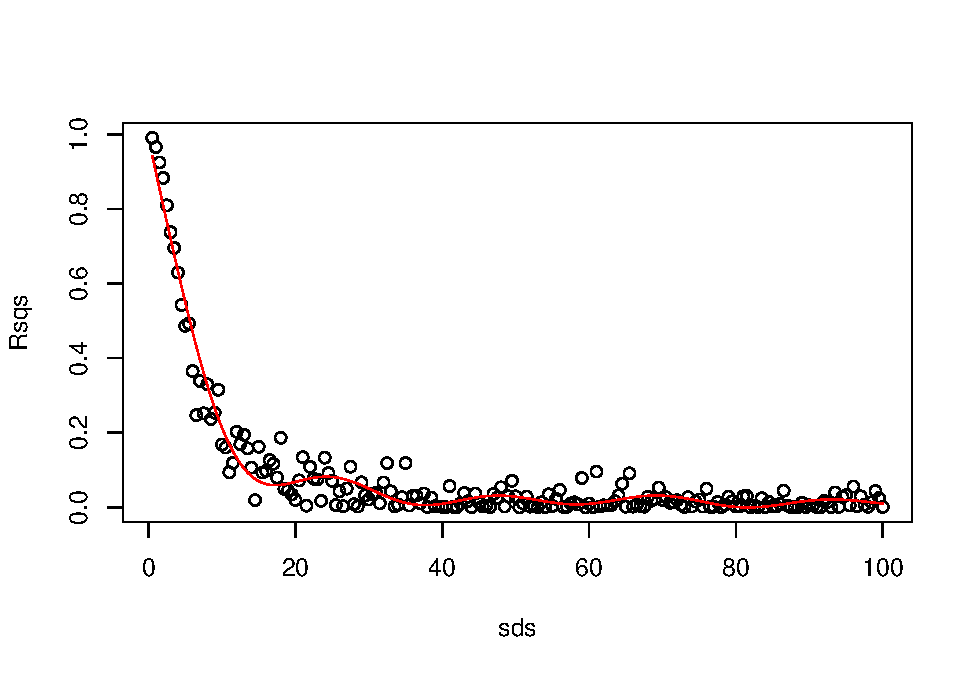
\includegraphics{ECOMODbook_files/figure-latex/a6.32-1.pdf}

Aha\ldots{} remember what we talked in class today? It seems like we have overfitted. Then, I constrain the GAM.

\begin{Shaded}
\begin{Highlighting}[]
\FunctionTok{library}\NormalTok{(mgcv)}
\NormalTok{gam1}\OtherTok{=}\FunctionTok{gam}\NormalTok{(Rsqs}\SpecialCharTok{\textasciitilde{}}\FunctionTok{s}\NormalTok{(sds,}\AttributeTok{k=}\DecValTok{3}\NormalTok{),}\AttributeTok{link=}\NormalTok{log)}
\CommentTok{\#make predictions to plot the estimated GAM model}
\NormalTok{predRsqs}\OtherTok{=}\FunctionTok{predict.gam}\NormalTok{(gam1,}\AttributeTok{newdata =} \FunctionTok{list}\NormalTok{(}\AttributeTok{sds=}\NormalTok{sds),}\AttributeTok{type=}\StringTok{"response"}\NormalTok{)}
\FunctionTok{plot}\NormalTok{(sds,Rsqs)}
\FunctionTok{lines}\NormalTok{(sds,predRsqs,}\AttributeTok{col=}\StringTok{"red"}\NormalTok{)}
\end{Highlighting}
\end{Shaded}

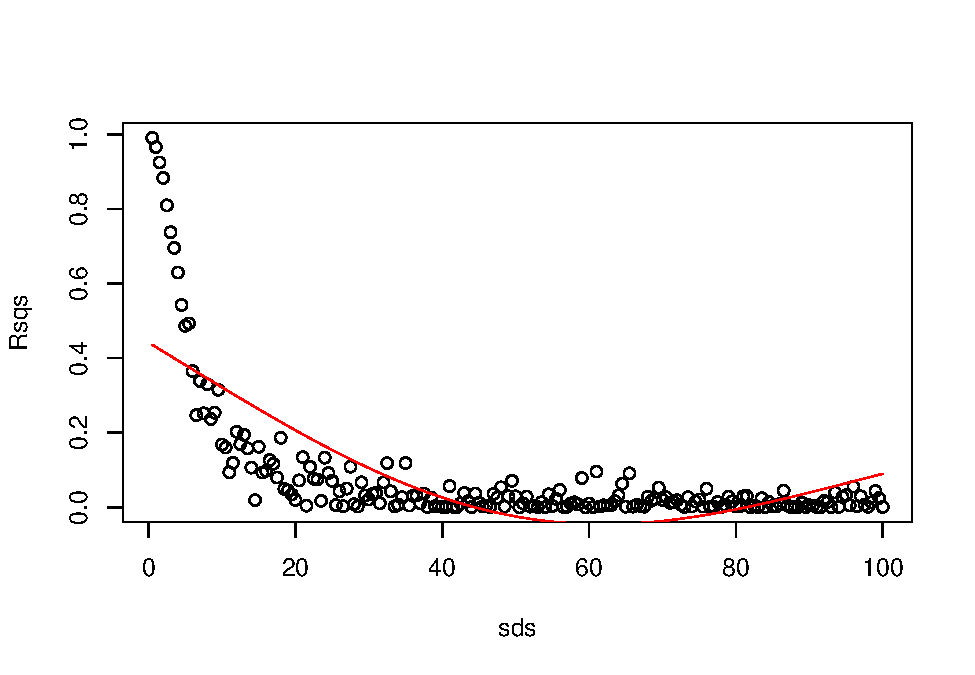
\includegraphics{ECOMODbook_files/figure-latex/a6.33-1.pdf}

That was too much\ldots{}

\begin{Shaded}
\begin{Highlighting}[]
\FunctionTok{library}\NormalTok{(mgcv)}
\NormalTok{gam1}\OtherTok{=}\FunctionTok{gam}\NormalTok{(Rsqs}\SpecialCharTok{\textasciitilde{}}\FunctionTok{s}\NormalTok{(sds,}\AttributeTok{k=}\DecValTok{6}\NormalTok{),}\AttributeTok{link=}\NormalTok{log)}
\CommentTok{\#make predictions to plot the estimated GAM model}
\NormalTok{predRsqs}\OtherTok{=}\FunctionTok{predict.gam}\NormalTok{(gam1,}\AttributeTok{newdata =} \FunctionTok{list}\NormalTok{(}\AttributeTok{sds=}\NormalTok{sds),}\AttributeTok{type=}\StringTok{"response"}\NormalTok{)}
\FunctionTok{plot}\NormalTok{(sds,Rsqs)}
\FunctionTok{lines}\NormalTok{(sds,predRsqs,}\AttributeTok{col=}\StringTok{"red"}\NormalTok{)}
\end{Highlighting}
\end{Shaded}

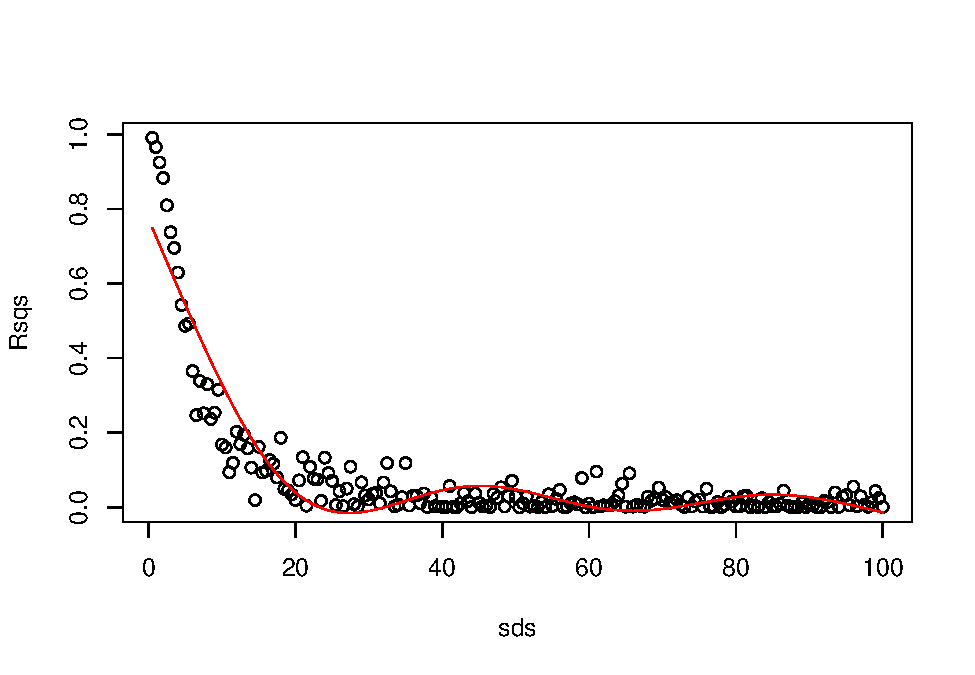
\includegraphics{ECOMODbook_files/figure-latex/a6.34-1.pdf}

That is already overfitting\ldots{} conclusion, the GAM is not the right tool here :)

What is\ldots? Well, stay tuned and one day you'll learn!

\hypertarget{aula7}{%
\chapter{Class 7 14 10 2020}\label{aula7}}

In this class we continue exploring regression models, but we are going to increase their complexity. No longer just \texttt{a+bx}, but we add more explanatory variables. In particular, we will also add a factor covariate. And then we look under the hood to what that means.

\hypertarget{task-1}{%
\section{Task 1}\label{task-1}}

The first task the students were faced was to use some code to explore, by simulation, the impact of having variables in the model that are not relevant to explain the response. In particular, we wanted to identify when there would be no errors, or when there would be type I (a variable not relevant to explain the response is found relevant) and type II (a relevant variable to explain the response is not considered relevant) errors. For the sake of this example we consider a significance level of 5\%, but remember there is nothing sacred about it.

The guidelines provided were: ``Using the code below, and while changing the \texttt{seed} (\texttt{******} to begin with, so the code does not run as is!), explore how changing the parameters and the error leads to different amounts of type I and type II errors.''

\begin{Shaded}
\begin{Highlighting}[]
\CommentTok{\# xs1 and xs2 wrong {-} type II error, xs3 and xs4 ok}
\NormalTok{seed}\OtherTok{\textless{}{-}}\ErrorTok{******}
\FunctionTok{set.seed}\NormalTok{(seed)}
\CommentTok{\#define parameters}
\NormalTok{n}\OtherTok{\textless{}{-}}\DecValTok{50}\NormalTok{;b0}\OtherTok{\textless{}{-}}\DecValTok{5}\NormalTok{;b1}\OtherTok{\textless{}{-}}\DecValTok{3}\NormalTok{;b2}\OtherTok{\textless{}{-}}\SpecialCharTok{{-}}\DecValTok{2}\NormalTok{;error }\OtherTok{\textless{}{-}} \DecValTok{4}
\CommentTok{\#simulate potential explanatory variables}
\NormalTok{xs1}\OtherTok{=}\FunctionTok{runif}\NormalTok{(n,}\DecValTok{10}\NormalTok{,}\DecValTok{20}\NormalTok{)}
\NormalTok{xs2}\OtherTok{=}\FunctionTok{runif}\NormalTok{(n,}\DecValTok{10}\NormalTok{,}\DecValTok{20}\NormalTok{)}
\NormalTok{xs3}\OtherTok{=}\FunctionTok{runif}\NormalTok{(n,}\DecValTok{10}\NormalTok{,}\DecValTok{20}\NormalTok{)}
\NormalTok{xs4}\OtherTok{=}\FunctionTok{runif}\NormalTok{(n,}\DecValTok{10}\NormalTok{,}\DecValTok{20}\NormalTok{)}
\CommentTok{\#simulate response}
\NormalTok{ys}\OtherTok{=}\NormalTok{b0}\SpecialCharTok{+}\NormalTok{b1}\SpecialCharTok{*}\NormalTok{xs1}\SpecialCharTok{{-}}\NormalTok{b2}\SpecialCharTok{*}\NormalTok{xs2}\SpecialCharTok{+}\FunctionTok{rnorm}\NormalTok{(n,}\AttributeTok{sd=}\NormalTok{error)}
\CommentTok{\#plot data}
\FunctionTok{plot}\NormalTok{(xs1,ys)}
\CommentTok{\#a model missing a variable, xs2}
\CommentTok{\#summary(lm(ys\textasciitilde{}xs1))}
\CommentTok{\#the true model}
\CommentTok{\#summary(lm(ys\textasciitilde{}xs1+xs2))}
\CommentTok{\#a model including irrelevant variables}
\FunctionTok{summary}\NormalTok{(}\FunctionTok{lm}\NormalTok{(ys}\SpecialCharTok{\textasciitilde{}}\NormalTok{xs1}\SpecialCharTok{+}\NormalTok{xs2}\SpecialCharTok{+}\NormalTok{xs3}\SpecialCharTok{+}\NormalTok{xs4))}
\end{Highlighting}
\end{Shaded}

The first thing to notice is that the model we simulate from only includes \texttt{xs1} and \texttt{xs2}. So, \texttt{xs3} and \texttt{xs4} do not have any impact on the response \texttt{y}

So we try different values for the seed and check what happens, Try \texttt{seed\textless{}-1}

\begin{Shaded}
\begin{Highlighting}[]
\NormalTok{seed}\OtherTok{\textless{}{-}}\DecValTok{1}
\FunctionTok{set.seed}\NormalTok{(seed)}
\CommentTok{\#define parameters}
\NormalTok{n}\OtherTok{\textless{}{-}}\DecValTok{50}\NormalTok{;b0}\OtherTok{\textless{}{-}}\DecValTok{5}\NormalTok{;b1}\OtherTok{\textless{}{-}}\DecValTok{3}\NormalTok{;b2}\OtherTok{\textless{}{-}}\SpecialCharTok{{-}}\DecValTok{2}\NormalTok{;error }\OtherTok{\textless{}{-}} \DecValTok{4}
\CommentTok{\#simulate potential explanatory variables}
\NormalTok{xs1}\OtherTok{=}\FunctionTok{runif}\NormalTok{(n,}\DecValTok{10}\NormalTok{,}\DecValTok{20}\NormalTok{)}
\NormalTok{xs2}\OtherTok{=}\FunctionTok{runif}\NormalTok{(n,}\DecValTok{10}\NormalTok{,}\DecValTok{20}\NormalTok{)}
\NormalTok{xs3}\OtherTok{=}\FunctionTok{runif}\NormalTok{(n,}\DecValTok{10}\NormalTok{,}\DecValTok{20}\NormalTok{)}
\NormalTok{xs4}\OtherTok{=}\FunctionTok{runif}\NormalTok{(n,}\DecValTok{10}\NormalTok{,}\DecValTok{20}\NormalTok{)}
\CommentTok{\#simulate response}
\NormalTok{ys}\OtherTok{=}\NormalTok{b0}\SpecialCharTok{+}\NormalTok{b1}\SpecialCharTok{*}\NormalTok{xs1}\SpecialCharTok{{-}}\NormalTok{b2}\SpecialCharTok{*}\NormalTok{xs2}\SpecialCharTok{+}\FunctionTok{rnorm}\NormalTok{(n,}\AttributeTok{sd=}\NormalTok{error)}
\CommentTok{\#plot data}
\FunctionTok{plot}\NormalTok{(xs1,ys)}
\CommentTok{\#look at model summary}
\FunctionTok{summary}\NormalTok{(}\FunctionTok{lm}\NormalTok{(ys}\SpecialCharTok{\textasciitilde{}}\NormalTok{xs1}\SpecialCharTok{+}\NormalTok{xs2}\SpecialCharTok{+}\NormalTok{xs3}\SpecialCharTok{+}\NormalTok{xs4))}
\end{Highlighting}
\end{Shaded}

All good, no errors. That is, \texttt{xs1} and \texttt{xs2} are considered statistically significant at th 5\% level and \texttt{xs3} and \texttt{xs4} are not found relevant to explain the response. Now, we keep changing \texttt{seed}

\begin{Shaded}
\begin{Highlighting}[]
\NormalTok{seed}\OtherTok{\textless{}{-}}\DecValTok{4}
\FunctionTok{set.seed}\NormalTok{(seed)}
\CommentTok{\#define parameters}
\NormalTok{n}\OtherTok{\textless{}{-}}\DecValTok{50}\NormalTok{;b0}\OtherTok{\textless{}{-}}\DecValTok{5}\NormalTok{;b1}\OtherTok{\textless{}{-}}\DecValTok{3}\NormalTok{;b2}\OtherTok{\textless{}{-}}\SpecialCharTok{{-}}\DecValTok{2}\NormalTok{;error }\OtherTok{\textless{}{-}} \DecValTok{4}
\CommentTok{\#simulate potential explanatory variables}
\NormalTok{xs1}\OtherTok{=}\FunctionTok{runif}\NormalTok{(n,}\DecValTok{10}\NormalTok{,}\DecValTok{20}\NormalTok{)}
\NormalTok{xs2}\OtherTok{=}\FunctionTok{runif}\NormalTok{(n,}\DecValTok{10}\NormalTok{,}\DecValTok{20}\NormalTok{)}
\NormalTok{xs3}\OtherTok{=}\FunctionTok{runif}\NormalTok{(n,}\DecValTok{10}\NormalTok{,}\DecValTok{20}\NormalTok{)}
\NormalTok{xs4}\OtherTok{=}\FunctionTok{runif}\NormalTok{(n,}\DecValTok{10}\NormalTok{,}\DecValTok{20}\NormalTok{)}
\CommentTok{\#simulate response}
\NormalTok{ys}\OtherTok{=}\NormalTok{b0}\SpecialCharTok{+}\NormalTok{b1}\SpecialCharTok{*}\NormalTok{xs1}\SpecialCharTok{{-}}\NormalTok{b2}\SpecialCharTok{*}\NormalTok{xs2}\SpecialCharTok{+}\FunctionTok{rnorm}\NormalTok{(n,}\AttributeTok{sd=}\NormalTok{error)}
\CommentTok{\#plot data}
\FunctionTok{plot}\NormalTok{(xs1,ys)}
\CommentTok{\#look at model summary}
\FunctionTok{summary}\NormalTok{(}\FunctionTok{lm}\NormalTok{(ys}\SpecialCharTok{\textasciitilde{}}\NormalTok{xs1}\SpecialCharTok{+}\NormalTok{xs2}\SpecialCharTok{+}\NormalTok{xs3}\SpecialCharTok{+}\NormalTok{xs4))}
\end{Highlighting}
\end{Shaded}

We find our first type I error, \texttt{xs4} is found statistically significant, but we know it has no effect on the response. The same happens with \texttt{seed} being e.g.~9, 10. When we try \texttt{seed\ \textless{}-\ 11} we get another type I error, this time on \texttt{xs4}

\begin{Shaded}
\begin{Highlighting}[]
\NormalTok{seed}\OtherTok{\textless{}{-}}\DecValTok{11}
\FunctionTok{set.seed}\NormalTok{(seed)}
\CommentTok{\#define parameters}
\NormalTok{n}\OtherTok{\textless{}{-}}\DecValTok{50}\NormalTok{;b0}\OtherTok{\textless{}{-}}\DecValTok{5}\NormalTok{;b1}\OtherTok{\textless{}{-}}\DecValTok{3}\NormalTok{;b2}\OtherTok{\textless{}{-}}\SpecialCharTok{{-}}\DecValTok{2}\NormalTok{;error }\OtherTok{\textless{}{-}} \DecValTok{4}
\CommentTok{\#simulate potential explanatory variables}
\NormalTok{xs1}\OtherTok{=}\FunctionTok{runif}\NormalTok{(n,}\DecValTok{10}\NormalTok{,}\DecValTok{20}\NormalTok{)}
\NormalTok{xs2}\OtherTok{=}\FunctionTok{runif}\NormalTok{(n,}\DecValTok{10}\NormalTok{,}\DecValTok{20}\NormalTok{)}
\NormalTok{xs3}\OtherTok{=}\FunctionTok{runif}\NormalTok{(n,}\DecValTok{10}\NormalTok{,}\DecValTok{20}\NormalTok{)}
\NormalTok{xs4}\OtherTok{=}\FunctionTok{runif}\NormalTok{(n,}\DecValTok{10}\NormalTok{,}\DecValTok{20}\NormalTok{)}
\CommentTok{\#simulate response}
\NormalTok{ys}\OtherTok{=}\NormalTok{b0}\SpecialCharTok{+}\NormalTok{b1}\SpecialCharTok{*}\NormalTok{xs1}\SpecialCharTok{{-}}\NormalTok{b2}\SpecialCharTok{*}\NormalTok{xs2}\SpecialCharTok{+}\FunctionTok{rnorm}\NormalTok{(n,}\AttributeTok{sd=}\NormalTok{error)}
\CommentTok{\#plot data}
\FunctionTok{plot}\NormalTok{(xs1,ys)}
\end{Highlighting}
\end{Shaded}

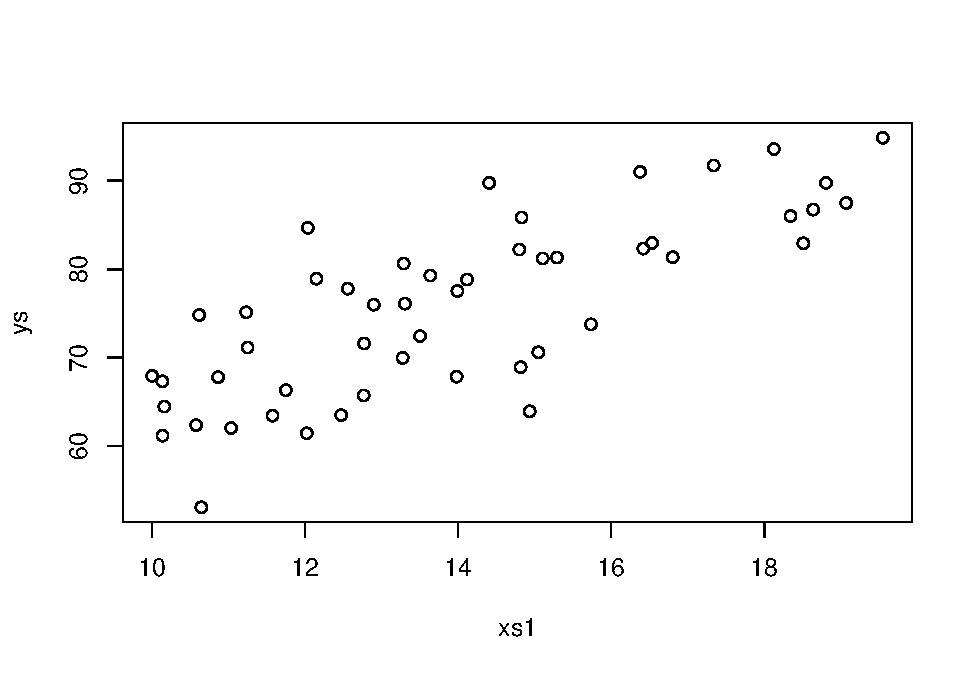
\includegraphics{ECOMODbook_files/figure-latex/a7.4-1.pdf}

\begin{Shaded}
\begin{Highlighting}[]
\CommentTok{\#look at model summary}
\FunctionTok{summary}\NormalTok{(}\FunctionTok{lm}\NormalTok{(ys}\SpecialCharTok{\textasciitilde{}}\NormalTok{xs1}\SpecialCharTok{+}\NormalTok{xs2}\SpecialCharTok{+}\NormalTok{xs3}\SpecialCharTok{+}\NormalTok{xs4))}
\end{Highlighting}
\end{Shaded}

\begin{verbatim}
## 
## Call:
## lm(formula = ys ~ xs1 + xs2 + xs3 + xs4)
## 
## Residuals:
##      Min       1Q   Median       3Q      Max 
## -10.3076  -2.7316   0.3072   2.2102   7.9088 
## 
## Coefficients:
##             Estimate Std. Error t value Pr(>|t|)    
## (Intercept) 16.44303    7.42710   2.214   0.0319 *  
## xs1          2.87327    0.21665  13.262  < 2e-16 ***
## xs2          1.93313    0.25274   7.649 1.12e-09 ***
## xs3         -0.47689    0.22325  -2.136   0.0381 *  
## xs4         -0.08922    0.20937  -0.426   0.6720    
## ---
## Signif. codes:  0 '***' 0.001 '**' 0.01 '*' 0.05 '.' 0.1 ' ' 1
## 
## Residual standard error: 4.074 on 45 degrees of freedom
## Multiple R-squared:  0.8484, Adjusted R-squared:  0.8349 
## F-statistic: 62.94 on 4 and 45 DF,  p-value: < 2.2e-16
\end{verbatim}

However, even after several runs, we never make a type II error. That must mean this setting has a large power, i.e.~the ability to detect a true effect when one exists. Well, there are many ways to decrease power, like having a smaller sample size, increase the error or lower the true effect. Let's try to increase the error, instead of the 4 used above, let's pump it up10 fold to 40

\begin{Shaded}
\begin{Highlighting}[]
\NormalTok{seed}\OtherTok{\textless{}{-}}\DecValTok{100}
\FunctionTok{set.seed}\NormalTok{(seed)}
\CommentTok{\#define parameters}
\NormalTok{n}\OtherTok{\textless{}{-}}\DecValTok{50}\NormalTok{;b0}\OtherTok{\textless{}{-}}\DecValTok{5}\NormalTok{;b1}\OtherTok{\textless{}{-}}\DecValTok{3}\NormalTok{;b2}\OtherTok{\textless{}{-}}\SpecialCharTok{{-}}\DecValTok{2}\NormalTok{;error }\OtherTok{\textless{}{-}} \DecValTok{40}
\CommentTok{\#simulate potential explanatory variables}
\NormalTok{xs1}\OtherTok{=}\FunctionTok{runif}\NormalTok{(n,}\DecValTok{10}\NormalTok{,}\DecValTok{20}\NormalTok{)}
\NormalTok{xs2}\OtherTok{=}\FunctionTok{runif}\NormalTok{(n,}\DecValTok{10}\NormalTok{,}\DecValTok{20}\NormalTok{)}
\NormalTok{xs3}\OtherTok{=}\FunctionTok{runif}\NormalTok{(n,}\DecValTok{10}\NormalTok{,}\DecValTok{20}\NormalTok{)}
\NormalTok{xs4}\OtherTok{=}\FunctionTok{runif}\NormalTok{(n,}\DecValTok{10}\NormalTok{,}\DecValTok{20}\NormalTok{)}
\CommentTok{\#simulate response}
\NormalTok{ys}\OtherTok{=}\NormalTok{b0}\SpecialCharTok{+}\NormalTok{b1}\SpecialCharTok{*}\NormalTok{xs1}\SpecialCharTok{{-}}\NormalTok{b2}\SpecialCharTok{*}\NormalTok{xs2}\SpecialCharTok{+}\FunctionTok{rnorm}\NormalTok{(n,}\AttributeTok{sd=}\NormalTok{error)}
\CommentTok{\#plot data}
\FunctionTok{plot}\NormalTok{(xs1,ys)}
\end{Highlighting}
\end{Shaded}

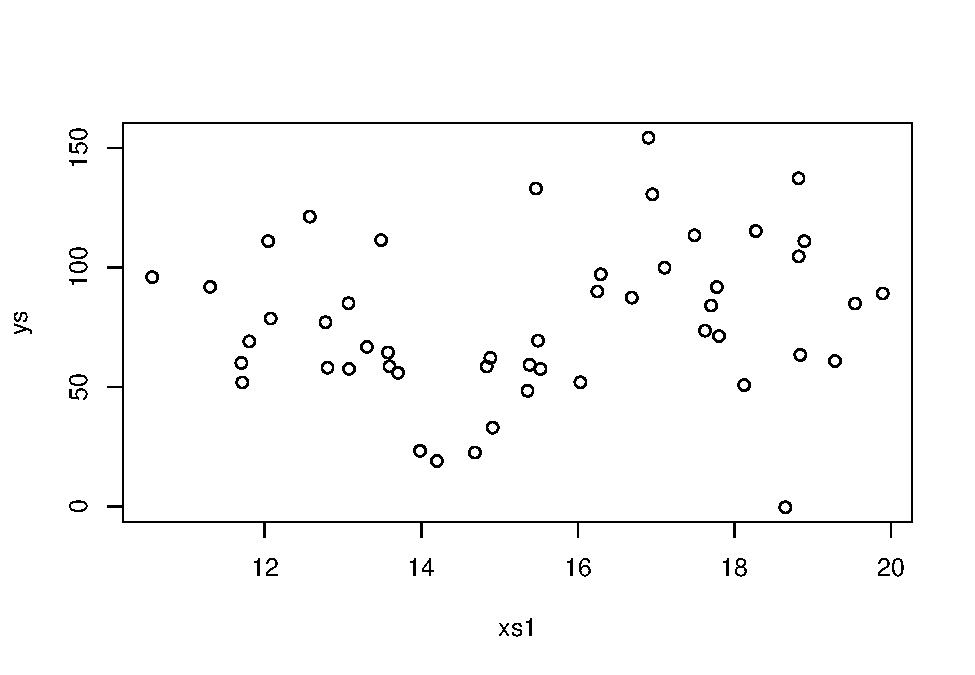
\includegraphics{ECOMODbook_files/figure-latex/a7.5-1.pdf}

\begin{Shaded}
\begin{Highlighting}[]
\CommentTok{\#look at model summary}
\FunctionTok{summary}\NormalTok{(}\FunctionTok{lm}\NormalTok{(ys}\SpecialCharTok{\textasciitilde{}}\NormalTok{xs1}\SpecialCharTok{+}\NormalTok{xs2}\SpecialCharTok{+}\NormalTok{xs3}\SpecialCharTok{+}\NormalTok{xs4))}
\end{Highlighting}
\end{Shaded}

\begin{verbatim}
## 
## Call:
## lm(formula = ys ~ xs1 + xs2 + xs3 + xs4)
## 
## Residuals:
##    Min     1Q Median     3Q    Max 
## -73.25 -17.86  -6.76  21.25  68.42 
## 
## Coefficients:
##             Estimate Std. Error t value Pr(>|t|)
## (Intercept)  22.8661    41.3133   0.553    0.583
## xs1           1.6034     1.8564   0.864    0.392
## xs2           0.9163     1.8092   0.506    0.615
## xs3           1.9650     1.6038   1.225    0.227
## xs4          -0.8544     1.7449  -0.490    0.627
## 
## Residual standard error: 32.4 on 45 degrees of freedom
## Multiple R-squared:  0.06896,    Adjusted R-squared:  -0.0138 
## F-statistic: 0.8333 on 4 and 45 DF,  p-value: 0.5112
\end{verbatim}

That was an overkill, now there is so much noise must seeds we use do not allow us to find an effect, let's cut that in half to 20

\begin{Shaded}
\begin{Highlighting}[]
\NormalTok{seed}\OtherTok{\textless{}{-}}\DecValTok{100}
\FunctionTok{set.seed}\NormalTok{(seed)}
\CommentTok{\#define parameters}
\NormalTok{n}\OtherTok{\textless{}{-}}\DecValTok{50}\NormalTok{;b0}\OtherTok{\textless{}{-}}\DecValTok{5}\NormalTok{;b1}\OtherTok{\textless{}{-}}\DecValTok{3}\NormalTok{;b2}\OtherTok{\textless{}{-}}\SpecialCharTok{{-}}\DecValTok{2}\NormalTok{;error }\OtherTok{\textless{}{-}} \DecValTok{20}
\CommentTok{\#simulate potential explanatory variables}
\NormalTok{xs1}\OtherTok{=}\FunctionTok{runif}\NormalTok{(n,}\DecValTok{10}\NormalTok{,}\DecValTok{20}\NormalTok{)}
\NormalTok{xs2}\OtherTok{=}\FunctionTok{runif}\NormalTok{(n,}\DecValTok{10}\NormalTok{,}\DecValTok{20}\NormalTok{)}
\NormalTok{xs3}\OtherTok{=}\FunctionTok{runif}\NormalTok{(n,}\DecValTok{10}\NormalTok{,}\DecValTok{20}\NormalTok{)}
\NormalTok{xs4}\OtherTok{=}\FunctionTok{runif}\NormalTok{(n,}\DecValTok{10}\NormalTok{,}\DecValTok{20}\NormalTok{)}
\CommentTok{\#simulate response}
\NormalTok{ys}\OtherTok{=}\NormalTok{b0}\SpecialCharTok{+}\NormalTok{b1}\SpecialCharTok{*}\NormalTok{xs1}\SpecialCharTok{{-}}\NormalTok{b2}\SpecialCharTok{*}\NormalTok{xs2}\SpecialCharTok{+}\FunctionTok{rnorm}\NormalTok{(n,}\AttributeTok{sd=}\NormalTok{error)}
\CommentTok{\#plot data}
\FunctionTok{plot}\NormalTok{(xs1,ys)}
\end{Highlighting}
\end{Shaded}

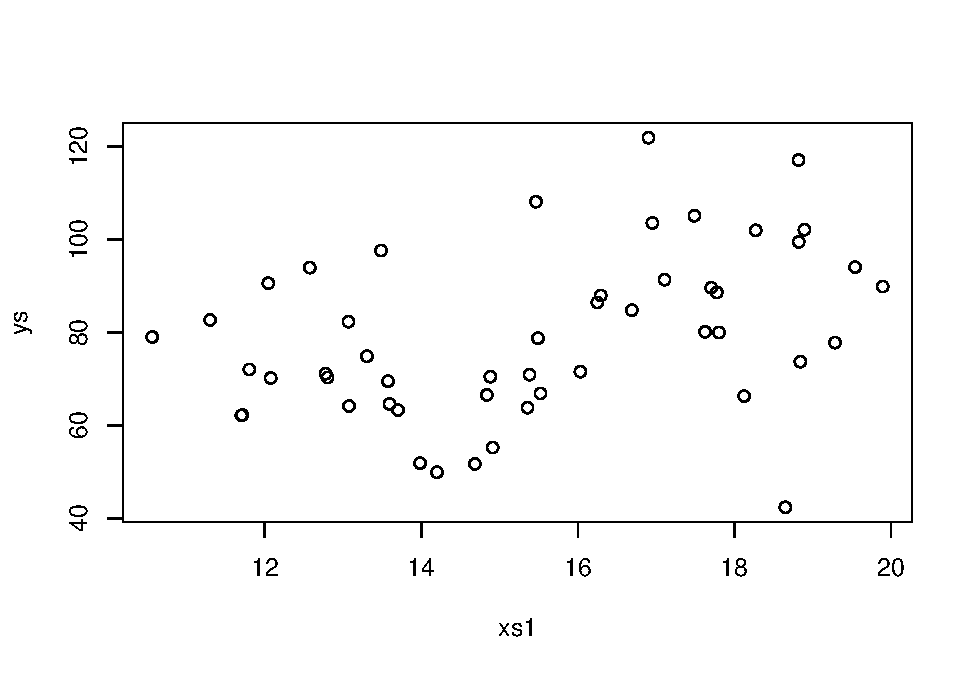
\includegraphics{ECOMODbook_files/figure-latex/a7.6-1.pdf}

\begin{Shaded}
\begin{Highlighting}[]
\CommentTok{\#look at model summary}
\FunctionTok{summary}\NormalTok{(}\FunctionTok{lm}\NormalTok{(ys}\SpecialCharTok{\textasciitilde{}}\NormalTok{xs1}\SpecialCharTok{+}\NormalTok{xs2}\SpecialCharTok{+}\NormalTok{xs3}\SpecialCharTok{+}\NormalTok{xs4))}
\end{Highlighting}
\end{Shaded}

\begin{verbatim}
## 
## Call:
## lm(formula = ys ~ xs1 + xs2 + xs3 + xs4)
## 
## Residuals:
##     Min      1Q  Median      3Q     Max 
## -36.624  -8.927  -3.380  10.623  34.211 
## 
## Coefficients:
##             Estimate Std. Error t value Pr(>|t|)  
## (Intercept)  13.9330    20.6566   0.675    0.503  
## xs1           2.3017     0.9282   2.480    0.017 *
## xs2           1.4582     0.9046   1.612    0.114  
## xs3           0.9825     0.8019   1.225    0.227  
## xs4          -0.4272     0.8724  -0.490    0.627  
## ---
## Signif. codes:  0 '***' 0.001 '**' 0.01 '*' 0.05 '.' 0.1 ' ' 1
## 
## Residual standard error: 16.2 on 45 degrees of freedom
## Multiple R-squared:  0.2262, Adjusted R-squared:  0.1574 
## F-statistic: 3.288 on 4 and 45 DF,  p-value: 0.01901
\end{verbatim}

back to all correct. Now, let's change seed again

\begin{Shaded}
\begin{Highlighting}[]
\NormalTok{seed}\OtherTok{\textless{}{-}}\DecValTok{103}
\FunctionTok{set.seed}\NormalTok{(seed)}
\CommentTok{\#define parameters}
\NormalTok{n}\OtherTok{\textless{}{-}}\DecValTok{50}\NormalTok{;b0}\OtherTok{\textless{}{-}}\DecValTok{5}\NormalTok{;b1}\OtherTok{\textless{}{-}}\DecValTok{3}\NormalTok{;b2}\OtherTok{\textless{}{-}}\SpecialCharTok{{-}}\DecValTok{2}\NormalTok{;error }\OtherTok{\textless{}{-}} \DecValTok{20}
\CommentTok{\#simulate potential explanatory variables}
\NormalTok{xs1}\OtherTok{=}\FunctionTok{runif}\NormalTok{(n,}\DecValTok{10}\NormalTok{,}\DecValTok{20}\NormalTok{)}
\NormalTok{xs2}\OtherTok{=}\FunctionTok{runif}\NormalTok{(n,}\DecValTok{10}\NormalTok{,}\DecValTok{20}\NormalTok{)}
\NormalTok{xs3}\OtherTok{=}\FunctionTok{runif}\NormalTok{(n,}\DecValTok{10}\NormalTok{,}\DecValTok{20}\NormalTok{)}
\NormalTok{xs4}\OtherTok{=}\FunctionTok{runif}\NormalTok{(n,}\DecValTok{10}\NormalTok{,}\DecValTok{20}\NormalTok{)}
\CommentTok{\#simulate response}
\NormalTok{ys}\OtherTok{=}\NormalTok{b0}\SpecialCharTok{+}\NormalTok{b1}\SpecialCharTok{*}\NormalTok{xs1}\SpecialCharTok{{-}}\NormalTok{b2}\SpecialCharTok{*}\NormalTok{xs2}\SpecialCharTok{+}\FunctionTok{rnorm}\NormalTok{(n,}\AttributeTok{sd=}\NormalTok{error)}
\CommentTok{\#plot data}
\FunctionTok{plot}\NormalTok{(xs1,ys)}
\end{Highlighting}
\end{Shaded}

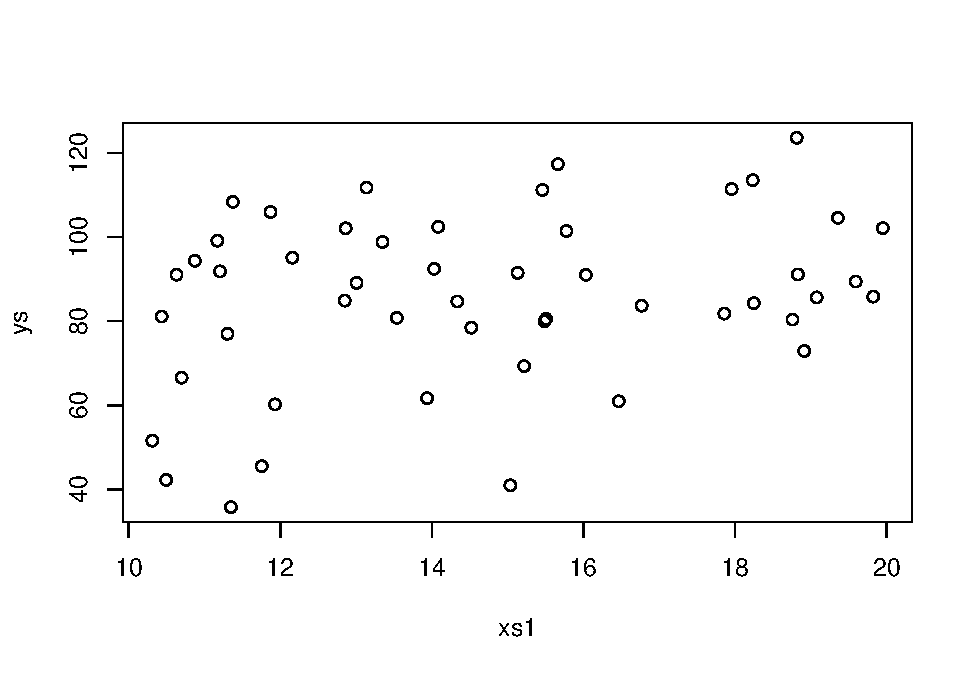
\includegraphics{ECOMODbook_files/figure-latex/a7.7-1.pdf}

\begin{Shaded}
\begin{Highlighting}[]
\CommentTok{\#look at model summary}
\FunctionTok{summary}\NormalTok{(}\FunctionTok{lm}\NormalTok{(ys}\SpecialCharTok{\textasciitilde{}}\NormalTok{xs1}\SpecialCharTok{+}\NormalTok{xs2}\SpecialCharTok{+}\NormalTok{xs3}\SpecialCharTok{+}\NormalTok{xs4))}
\end{Highlighting}
\end{Shaded}

\begin{verbatim}
## 
## Call:
## lm(formula = ys ~ xs1 + xs2 + xs3 + xs4)
## 
## Residuals:
##     Min      1Q  Median      3Q     Max 
## -36.079 -10.686  -0.148  16.413  33.845 
## 
## Coefficients:
##             Estimate Std. Error t value Pr(>|t|)  
## (Intercept)  9.70575   33.83339   0.287   0.7755  
## xs1          2.32559    0.93980   2.475   0.0172 *
## xs2          1.97688    1.20464   1.641   0.1078  
## xs3          0.69013    1.02110   0.676   0.5026  
## xs4          0.08031    0.97427   0.082   0.9347  
## ---
## Signif. codes:  0 '***' 0.001 '**' 0.01 '*' 0.05 '.' 0.1 ' ' 1
## 
## Residual standard error: 19.6 on 45 degrees of freedom
## Multiple R-squared:  0.1524, Adjusted R-squared:  0.07706 
## F-statistic: 2.023 on 4 and 45 DF,  p-value: 0.1073
\end{verbatim}

Bang on, a type II error, as \texttt{xs2} is no longer considered statistically significant. I am sure you can now play with the relevant model parameters, \texttt{b1}, \texttt{b2}, to incleare and decreese the actual effect, and with sample size \texttt{n} or as above with the \texttt{error} and explore the consequences of changing the balance in effect size, error and sample size on the ability of incurring in errors when doing regression. But remmeber the key, the reason we are able to see if an error is made or not is because we simulated reality. In this case, as it is never the case in an ecological dataset, we know the true model, which was

\[y=\beta_0+\beta_1 xs_1+\beta_2 xs2\]

That is the luxury of simulation, allowing you to test scenarios where ``reality'' is known, hence evaluating methods performance.

\begin{Shaded}
\begin{Highlighting}[]
\NormalTok{folder}\OtherTok{\textless{}{-}}\StringTok{"extfiles/"}
\CommentTok{\#folder\textless{}{-}"../Aula7 14 10 2020/"}
\NormalTok{d4l }\OtherTok{\textless{}{-}} \FunctionTok{read.csv}\NormalTok{(}\AttributeTok{file=}\FunctionTok{paste0}\NormalTok{(folder,}\StringTok{"data4lines.csv"}\NormalTok{))}
\NormalTok{n }\OtherTok{\textless{}{-}} \FunctionTok{nrow}\NormalTok{(d4l)}
\end{Highlighting}
\end{Shaded}

\hypertarget{task-2}{%
\section{Task 2}\label{task-2}}

The second task the students were faced was to create some regression data and the explore fitting models to it.

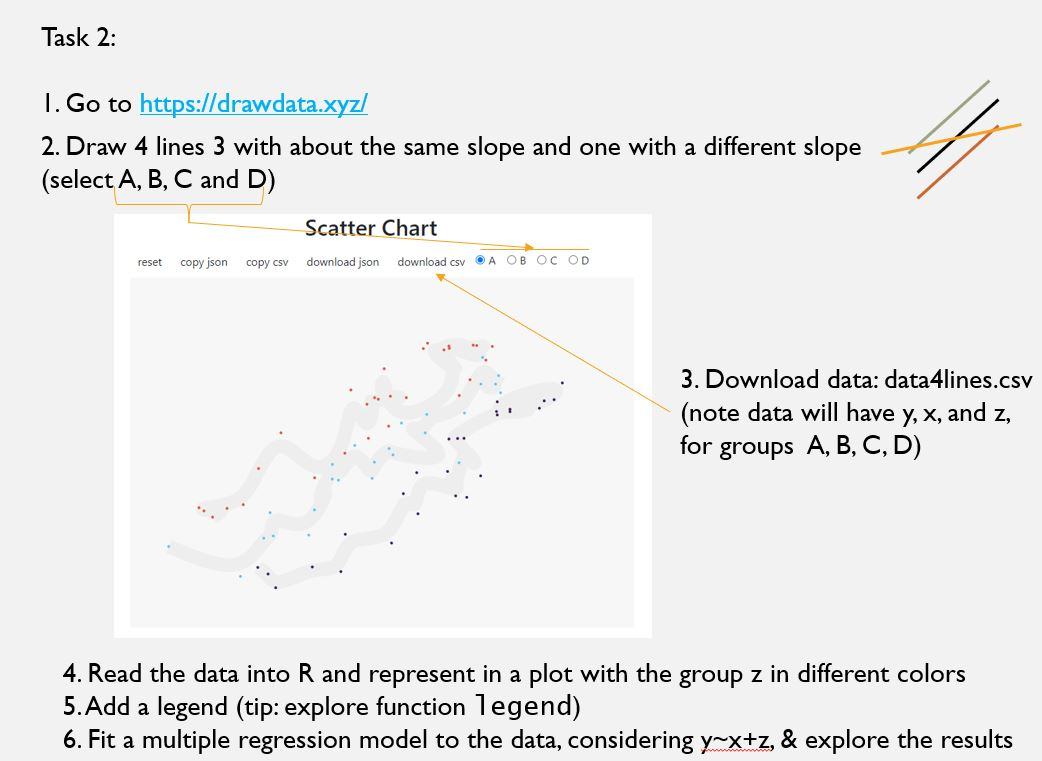
\includegraphics{extfiles/Aula7Task7.JPG}

The data was simulated via this website: \url{https://drawdata.xyz/} and was named \texttt{data4lines.csv}. Each student had its own dataset, here I work with my example.

We begin by reading the data in and plot it

\begin{Shaded}
\begin{Highlighting}[]
\CommentTok{\#read the data}
\CommentTok{\#folder\textless{}{-}"../Aula7 14 10 2020/"}
\NormalTok{folder}\OtherTok{\textless{}{-}}\StringTok{"extfiles/"}
\NormalTok{data4lines }\OtherTok{\textless{}{-}} \FunctionTok{read.csv}\NormalTok{(}\AttributeTok{file=}\FunctionTok{paste0}\NormalTok{(folder,}\StringTok{"data4lines.csv"}\NormalTok{))}
\CommentTok{\#plot all the data}
\FunctionTok{plot}\NormalTok{(y}\SpecialCharTok{\textasciitilde{}}\NormalTok{x,}\AttributeTok{data=}\NormalTok{data4lines)}
\end{Highlighting}
\end{Shaded}

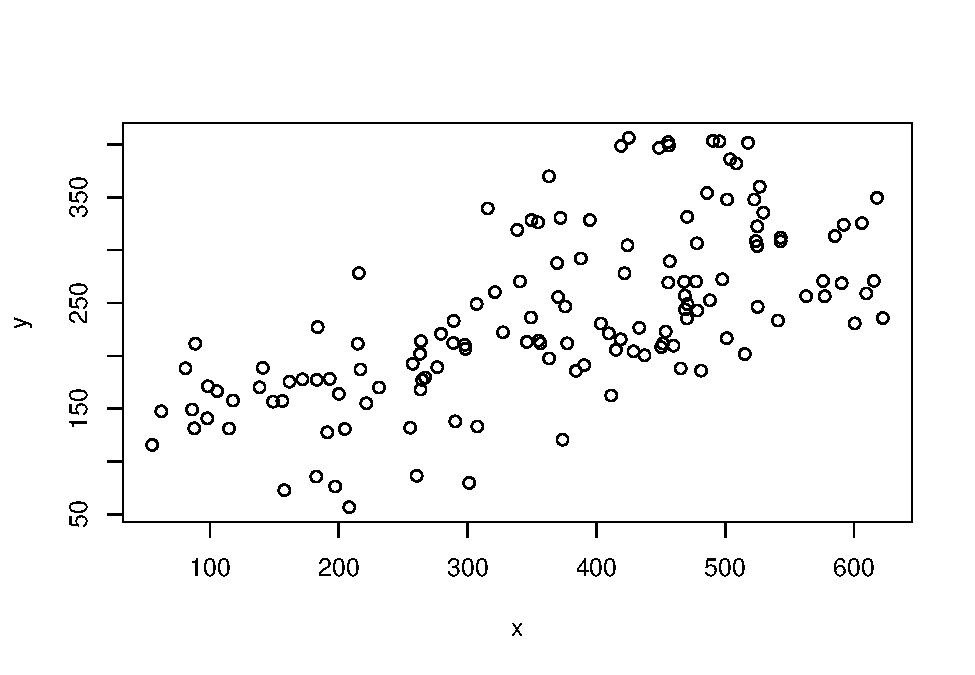
\includegraphics{ECOMODbook_files/figure-latex/a7.9-1.pdf}

Now, to turn this a bit more interesting, we come up with a narrative.

These correspond to observations from weights and lenghts of a sample of animals, fish from the species \emph{Fishus inventadicus}. We could fit a regression line to this data and see if we can predict weight from length

\begin{Shaded}
\begin{Highlighting}[]
\CommentTok{\#plot all the data}
\FunctionTok{plot}\NormalTok{(y}\SpecialCharTok{\textasciitilde{}}\NormalTok{x,}\AttributeTok{data=}\NormalTok{data4lines)}
\CommentTok{\#fit model to pooled data}
\NormalTok{lmlinesG}\OtherTok{\textless{}{-}}\FunctionTok{lm}\NormalTok{(y}\SpecialCharTok{\textasciitilde{}}\NormalTok{x,}\AttributeTok{data=}\NormalTok{data4lines)}
\FunctionTok{abline}\NormalTok{(lmlinesG,}\AttributeTok{lwd=}\DecValTok{3}\NormalTok{,}\AttributeTok{lty=}\DecValTok{2}\NormalTok{)}
\end{Highlighting}
\end{Shaded}

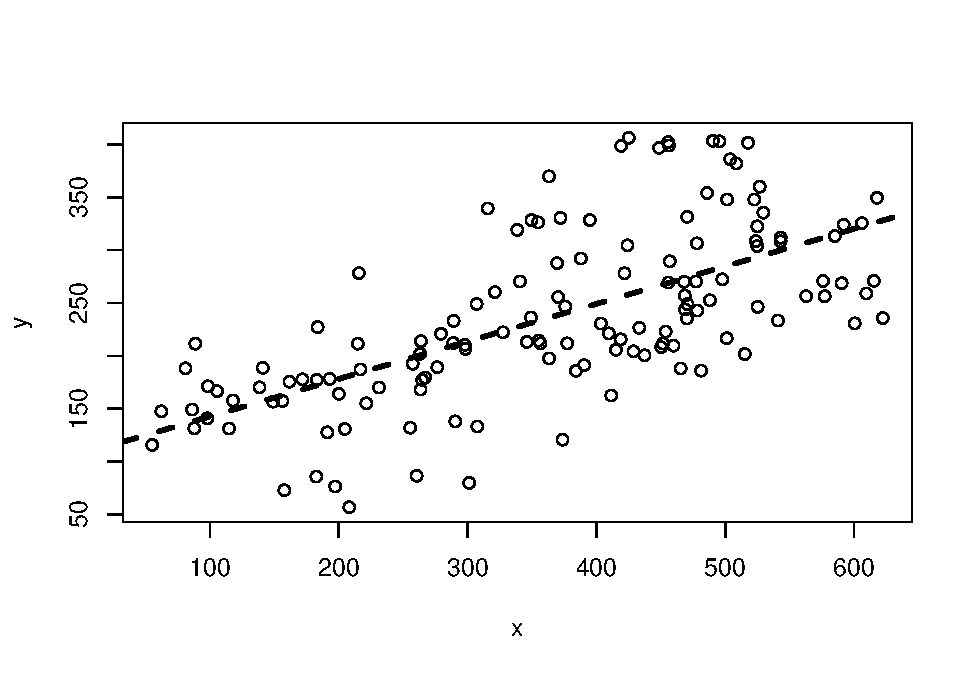
\includegraphics{ECOMODbook_files/figure-latex/a7.10-1.pdf}

\begin{Shaded}
\begin{Highlighting}[]
\FunctionTok{summary}\NormalTok{(lmlinesG)}
\end{Highlighting}
\end{Shaded}

\begin{verbatim}
## 
## Call:
## lm(formula = y ~ x, data = data4lines)
## 
## Residuals:
##      Min       1Q   Median       3Q      Max 
## -134.304  -44.188   -1.995   29.432  148.202 
## 
## Coefficients:
##              Estimate Std. Error t value Pr(>|t|)    
## (Intercept) 107.17590   14.03069   7.639 3.51e-12 ***
## x             0.35513    0.03553   9.995  < 2e-16 ***
## ---
## Signif. codes:  0 '***' 0.001 '**' 0.01 '*' 0.05 '.' 0.1 ' ' 1
## 
## Residual standard error: 61.78 on 136 degrees of freedom
## Multiple R-squared:  0.4235, Adjusted R-squared:  0.4193 
## F-statistic: 99.91 on 1 and 136 DF,  p-value: < 2.2e-16
\end{verbatim}

and it looks like we can indeed predict the weight of the species from its length. The length is higly statistically significant. Not surprisingly, the longer the fish the heavier it is.

Now, the plot thickens. These animals actually came from 4 different museums, and are assumed to be the same species. However, a scientis decides to look at wether there are differences in the data from the 4 museums. So he colours the data by museum

\begin{Shaded}
\begin{Highlighting}[]
\CommentTok{\#plot all the data}
\FunctionTok{plot}\NormalTok{(y}\SpecialCharTok{\textasciitilde{}}\NormalTok{x,}\AttributeTok{col=}\FunctionTok{as.numeric}\NormalTok{(}\FunctionTok{as.factor}\NormalTok{(z)),}\AttributeTok{data=}\NormalTok{data4lines,}\AttributeTok{pch=}\DecValTok{1}\NormalTok{)}
\FunctionTok{legend}\NormalTok{(}\StringTok{"topleft"}\NormalTok{,}\AttributeTok{inset=}\FloatTok{0.05}\NormalTok{,}\AttributeTok{legend=}\NormalTok{letters[}\DecValTok{1}\SpecialCharTok{:}\DecValTok{4}\NormalTok{],}\AttributeTok{col=}\DecValTok{1}\SpecialCharTok{:}\DecValTok{4}\NormalTok{,}\AttributeTok{pch=}\DecValTok{1}\NormalTok{)}
\end{Highlighting}
\end{Shaded}

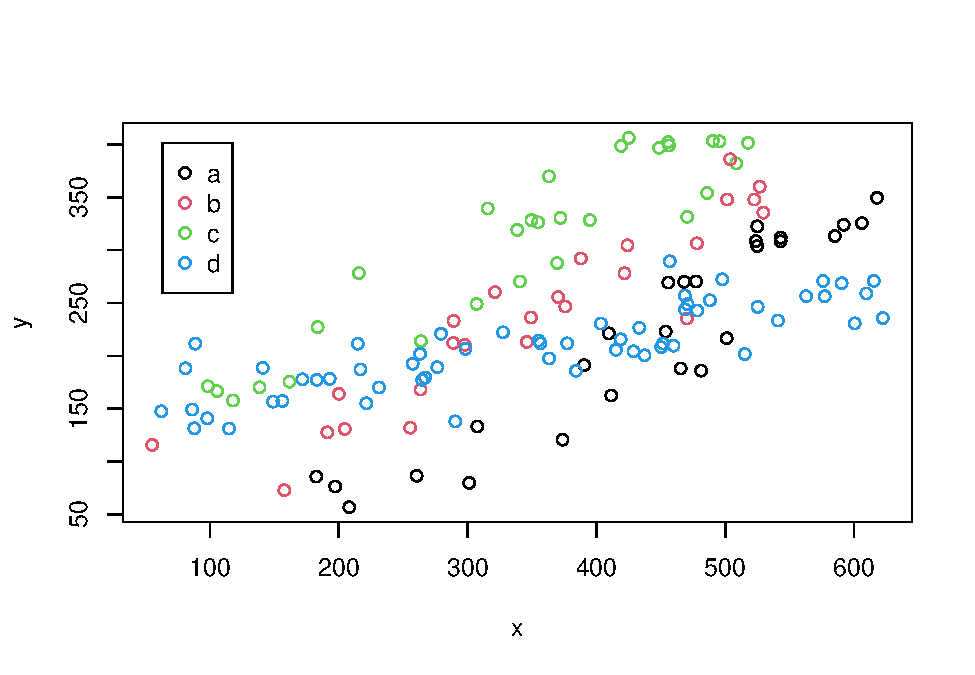
\includegraphics{ECOMODbook_files/figure-latex/a7.11-1.pdf}

We see a patter in the data, the data from the different museums tend to cluster. He decides to investigate. Note folks providing names to museum in this country are a bit borring, and the museums are called ``a'', ``b'', ``c'' and ``d''.

Our smart researcher says: ``well, it seems like the relationship might be different in each museum''. Then, maybe I should fit a model that includes museum as a covariate \texttt{weight\textasciitilde{}length+museum}.

\[y=\beta_0+\beta_1 \times length +\beta_2 \times museum\]

And so he does and plots it

\begin{Shaded}
\begin{Highlighting}[]
\CommentTok{\#fit model per group}
\NormalTok{lmlines}\OtherTok{\textless{}{-}}\FunctionTok{lm}\NormalTok{(y}\SpecialCharTok{\textasciitilde{}}\NormalTok{x}\SpecialCharTok{+}\NormalTok{z,}\AttributeTok{data=}\NormalTok{data4lines)}
\FunctionTok{summary}\NormalTok{(lmlines)}
\end{Highlighting}
\end{Shaded}

\begin{verbatim}
## 
## Call:
## lm(formula = y ~ x + z, data = data4lines)
## 
## Residuals:
##    Min     1Q Median     3Q    Max 
## -90.01 -35.01   2.54  35.51 108.10 
## 
## Coefficients:
##              Estimate Std. Error t value Pr(>|t|)    
## (Intercept)  45.51813   13.83069   3.291  0.00128 ** 
## x             0.39657    0.02516  15.763  < 2e-16 ***
## zb           54.92376   12.11597   4.533 1.28e-05 ***
## zc          128.20339   11.72572  10.934  < 2e-16 ***
## zd           22.82412   10.26509   2.223  0.02787 *  
## ---
## Signif. codes:  0 '***' 0.001 '**' 0.01 '*' 0.05 '.' 0.1 ' ' 1
## 
## Residual standard error: 42.5 on 133 degrees of freedom
## Multiple R-squared:  0.7332, Adjusted R-squared:  0.7252 
## F-statistic: 91.38 on 4 and 133 DF,  p-value: < 2.2e-16
\end{verbatim}

The output shows that the length is relevant, but the museum is relevant too. The relationship might be different per museum! In the output we see the \texttt{x}, the length, but not the \texttt{z}, it has been transformed into \texttt{zb}, \texttt{zc} and \texttt{zd}. Why is that? That is a mistery that we shall unfold now!

While the model we are fitting might be represented by \texttt{weight\textasciitilde{}length+museum}, th edesign matrix being fitted replaces the \texttt{museum} (a factor with 4 levels) with 3 dummy variables (a factor with k levels required k-1 dummy variables). So the real model being fitted is really

\[y=\beta_0+\beta_1 \times length + \beta_{2b} \times zb + \beta_{2c} \times zc + \beta_{2d} \times zd\]

Wait, but where is the level \texttt{a}? It is in the intercept, and if I had an euro for each time that confused a student, I would not be here but in a beach in the Bahamas having a piña colada :)

But let's unfold the mistery, shall we? By default, R takes 1 level of (each/a) factor and uses it as the intercept. Here it used \texttt{a} (the choice is in this case by alphabetical ored, but one can change that, which might be useful if e.g.~you want to have as the intercept a control level, say; look e.g.~into function \texttt{factor} help to see how you can change the baseline \texttt{level} of a factor).

Hence, the intercept for museum \texttt{a} is 45.5181335. What about the intercep of the othe rmuseums? They are always reported with \texttt{a} as the reference. Look at the equation above, what happens when say zc is 1 and zd and zb are 0, it becomes

\[y=\beta_0+\beta_1 \times length + \beta_{2c} \times zc \]
\[y=(\beta_0+\beta_{2c})+\beta_1 \times length = intercep + slope \times length\]

and so, from the above output, that equates to \texttt{y=lmlines\$coefficients{[}1{]}+lmlines\$coefficients{[}4{]},lmlines\$coefficients{[}2{]}} or 173.7215247+0.3965715 \(\times\) \texttt{length}.

So now we can add all these estimated regression lines to the plot

\begin{Shaded}
\begin{Highlighting}[]
\CommentTok{\#plot all}
\FunctionTok{plot}\NormalTok{(y}\SpecialCharTok{\textasciitilde{}}\NormalTok{x,}\AttributeTok{col=}\FunctionTok{as.numeric}\NormalTok{(}\FunctionTok{as.factor}\NormalTok{(z)),}\AttributeTok{data=}\NormalTok{data4lines)}
\FunctionTok{legend}\NormalTok{(}\StringTok{"topleft"}\NormalTok{,}\AttributeTok{inset=}\FloatTok{0.05}\NormalTok{,}\AttributeTok{legend=}\FunctionTok{c}\NormalTok{(LETTERS[}\DecValTok{1}\SpecialCharTok{:}\DecValTok{4}\NormalTok{],}\StringTok{"all"}\NormalTok{),}\AttributeTok{col=}\FunctionTok{c}\NormalTok{(}\DecValTok{1}\SpecialCharTok{:}\DecValTok{4}\NormalTok{,}\DecValTok{1}\NormalTok{),}\AttributeTok{lty=}\FunctionTok{c}\NormalTok{(}\FunctionTok{rep}\NormalTok{(}\DecValTok{1}\NormalTok{,}\DecValTok{4}\NormalTok{),}\DecValTok{2}\NormalTok{),}\AttributeTok{lwd=}\FunctionTok{c}\NormalTok{(}\FunctionTok{rep}\NormalTok{(}\DecValTok{1}\NormalTok{,}\DecValTok{4}\NormalTok{),}\DecValTok{3}\NormalTok{))}
\CommentTok{\#these are the wrong lines... why?}
\FunctionTok{abline}\NormalTok{(lmlinesG,}\AttributeTok{lwd=}\DecValTok{3}\NormalTok{,}\AttributeTok{lty=}\DecValTok{2}\NormalTok{)}
\FunctionTok{abline}\NormalTok{(lmlines}\SpecialCharTok{$}\NormalTok{coefficients[}\DecValTok{1}\NormalTok{],lmlines}\SpecialCharTok{$}\NormalTok{coefficients[}\DecValTok{2}\NormalTok{],}\AttributeTok{col=}\DecValTok{1}\NormalTok{)}
\FunctionTok{abline}\NormalTok{(lmlines}\SpecialCharTok{$}\NormalTok{coefficients[}\DecValTok{1}\NormalTok{]}\SpecialCharTok{+}\NormalTok{lmlines}\SpecialCharTok{$}\NormalTok{coefficients[}\DecValTok{3}\NormalTok{],lmlines}\SpecialCharTok{$}\NormalTok{coefficients[}\DecValTok{2}\NormalTok{],}\AttributeTok{col=}\DecValTok{2}\NormalTok{)}
\FunctionTok{abline}\NormalTok{(lmlines}\SpecialCharTok{$}\NormalTok{coefficients[}\DecValTok{1}\NormalTok{]}\SpecialCharTok{+}\NormalTok{lmlines}\SpecialCharTok{$}\NormalTok{coefficients[}\DecValTok{4}\NormalTok{],lmlines}\SpecialCharTok{$}\NormalTok{coefficients[}\DecValTok{2}\NormalTok{],}\AttributeTok{col=}\DecValTok{3}\NormalTok{)}
\FunctionTok{abline}\NormalTok{(lmlines}\SpecialCharTok{$}\NormalTok{coefficients[}\DecValTok{1}\NormalTok{]}\SpecialCharTok{+}\NormalTok{lmlines}\SpecialCharTok{$}\NormalTok{coefficients[}\DecValTok{5}\NormalTok{],lmlines}\SpecialCharTok{$}\NormalTok{coefficients[}\DecValTok{2}\NormalTok{],}\AttributeTok{col=}\DecValTok{4}\NormalTok{)}
\end{Highlighting}
\end{Shaded}

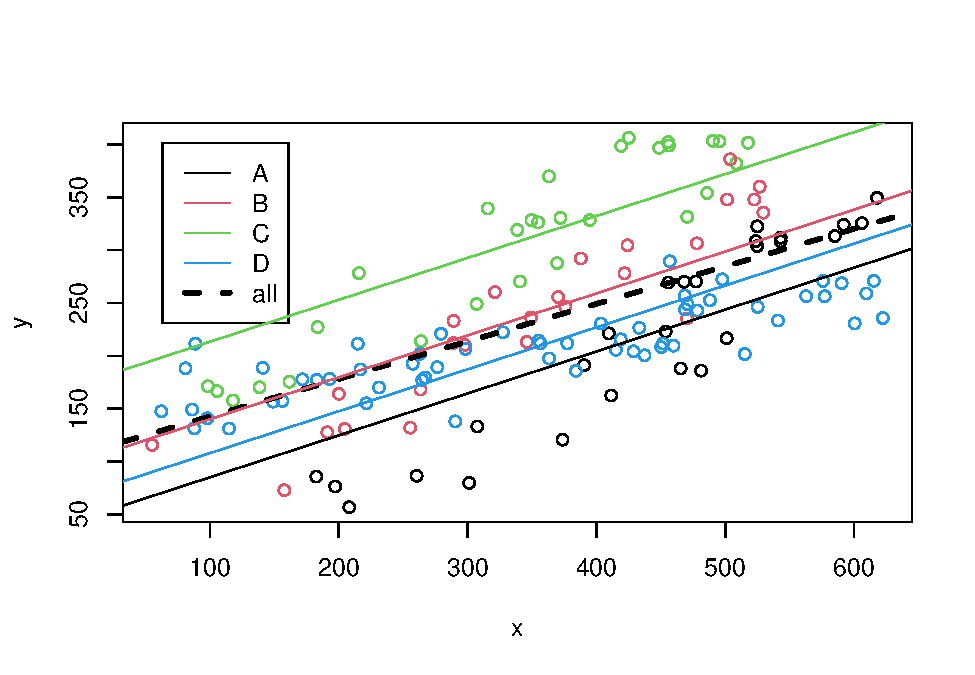
\includegraphics{ECOMODbook_files/figure-latex/a7.13-1.pdf}

note that, not surprisingly, all these lines have the same slope. Or in other words, the model we considered assumes that the slope of the model is the same across museums (which, remember, we know if not true!). We can easily check that the intercepts (i.e.~where the lines cross when length=x=0) of all lines are indeed easy to get from the model's output

\begin{Shaded}
\begin{Highlighting}[]
\CommentTok{\#plot all}
\FunctionTok{plot}\NormalTok{(y}\SpecialCharTok{\textasciitilde{}}\NormalTok{x,}\AttributeTok{xlim=}\FunctionTok{c}\NormalTok{(}\SpecialCharTok{{-}}\DecValTok{10}\NormalTok{,}\DecValTok{700}\NormalTok{),}\AttributeTok{ylim=}\FunctionTok{c}\NormalTok{(}\DecValTok{0}\NormalTok{,}\DecValTok{450}\NormalTok{),}\AttributeTok{col=}\FunctionTok{as.numeric}\NormalTok{(}\FunctionTok{as.factor}\NormalTok{(z)),}\AttributeTok{data=}\NormalTok{data4lines)}
\FunctionTok{legend}\NormalTok{(}\StringTok{"topleft"}\NormalTok{,}\AttributeTok{inset=}\FloatTok{0.05}\NormalTok{,}\AttributeTok{legend=}\FunctionTok{c}\NormalTok{(LETTERS[}\DecValTok{1}\SpecialCharTok{:}\DecValTok{4}\NormalTok{],}\StringTok{"all"}\NormalTok{),}\AttributeTok{col=}\FunctionTok{c}\NormalTok{(}\DecValTok{1}\SpecialCharTok{:}\DecValTok{4}\NormalTok{,}\DecValTok{1}\NormalTok{),}\AttributeTok{lty=}\FunctionTok{c}\NormalTok{(}\FunctionTok{rep}\NormalTok{(}\DecValTok{1}\NormalTok{,}\DecValTok{4}\NormalTok{),}\DecValTok{2}\NormalTok{),}\AttributeTok{lwd=}\FunctionTok{c}\NormalTok{(}\FunctionTok{rep}\NormalTok{(}\DecValTok{1}\NormalTok{,}\DecValTok{4}\NormalTok{),}\DecValTok{3}\NormalTok{))}
\CommentTok{\#these are the wrong lines... why?}
\FunctionTok{abline}\NormalTok{(lmlinesG,}\AttributeTok{lwd=}\DecValTok{3}\NormalTok{,}\AttributeTok{lty=}\DecValTok{2}\NormalTok{)}
\FunctionTok{abline}\NormalTok{(lmlines}\SpecialCharTok{$}\NormalTok{coefficients[}\DecValTok{1}\NormalTok{],lmlines}\SpecialCharTok{$}\NormalTok{coefficients[}\DecValTok{2}\NormalTok{],}\AttributeTok{col=}\DecValTok{1}\NormalTok{)}
\FunctionTok{abline}\NormalTok{(lmlines}\SpecialCharTok{$}\NormalTok{coefficients[}\DecValTok{1}\NormalTok{]}\SpecialCharTok{+}\NormalTok{lmlines}\SpecialCharTok{$}\NormalTok{coefficients[}\DecValTok{3}\NormalTok{],lmlines}\SpecialCharTok{$}\NormalTok{coefficients[}\DecValTok{2}\NormalTok{],}\AttributeTok{col=}\DecValTok{2}\NormalTok{)}
\FunctionTok{abline}\NormalTok{(lmlines}\SpecialCharTok{$}\NormalTok{coefficients[}\DecValTok{1}\NormalTok{]}\SpecialCharTok{+}\NormalTok{lmlines}\SpecialCharTok{$}\NormalTok{coefficients[}\DecValTok{4}\NormalTok{],lmlines}\SpecialCharTok{$}\NormalTok{coefficients[}\DecValTok{2}\NormalTok{],}\AttributeTok{col=}\DecValTok{3}\NormalTok{)}
\FunctionTok{abline}\NormalTok{(lmlines}\SpecialCharTok{$}\NormalTok{coefficients[}\DecValTok{1}\NormalTok{]}\SpecialCharTok{+}\NormalTok{lmlines}\SpecialCharTok{$}\NormalTok{coefficients[}\DecValTok{5}\NormalTok{],lmlines}\SpecialCharTok{$}\NormalTok{coefficients[}\DecValTok{2}\NormalTok{],}\AttributeTok{col=}\DecValTok{4}\NormalTok{)}


\FunctionTok{abline}\NormalTok{(}\AttributeTok{v=}\DecValTok{0}\NormalTok{,}\AttributeTok{lty=}\DecValTok{2}\NormalTok{)}
\FunctionTok{abline}\NormalTok{(}\AttributeTok{h=}\FloatTok{45.51813}\NormalTok{,}\AttributeTok{lty=}\DecValTok{2}\NormalTok{,}\AttributeTok{col=}\DecValTok{1}\NormalTok{)}
\FunctionTok{abline}\NormalTok{(}\AttributeTok{h=}\FloatTok{45.51813+54.92376}\NormalTok{,}\AttributeTok{lty=}\DecValTok{2}\NormalTok{,}\AttributeTok{col=}\DecValTok{2}\NormalTok{)}
\FunctionTok{abline}\NormalTok{(}\AttributeTok{h=}\FloatTok{45.51813+128.20339}\NormalTok{,}\AttributeTok{lty=}\DecValTok{2}\NormalTok{,}\AttributeTok{col=}\DecValTok{3}\NormalTok{)}
\FunctionTok{abline}\NormalTok{(}\AttributeTok{h=}\FloatTok{45.51813+22.82412}\NormalTok{,}\AttributeTok{lty=}\DecValTok{2}\NormalTok{,}\AttributeTok{col=}\DecValTok{4}\NormalTok{)}
\end{Highlighting}
\end{Shaded}

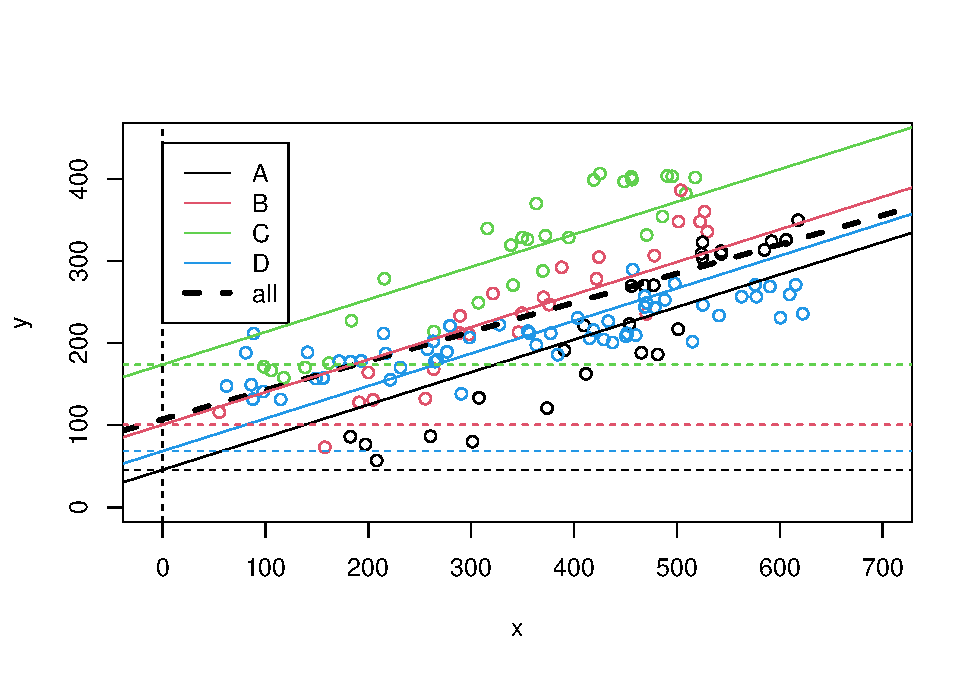
\includegraphics{ECOMODbook_files/figure-latex/a7.14-1.pdf}

Now, the smart biologist then says that he could also fit a separate line to each museum's data. And so he does, and that looks like this:

\begin{Shaded}
\begin{Highlighting}[]
\CommentTok{\#plot all the data}
\FunctionTok{plot}\NormalTok{(y}\SpecialCharTok{\textasciitilde{}}\NormalTok{x,}\AttributeTok{col=}\FunctionTok{as.numeric}\NormalTok{(}\FunctionTok{as.factor}\NormalTok{(z)),}\AttributeTok{data=}\NormalTok{data4lines,}\AttributeTok{pch=}\DecValTok{1}\NormalTok{)}
\CommentTok{\#completely independet regression lines}
\FunctionTok{abline}\NormalTok{(}\FunctionTok{lm}\NormalTok{(y}\SpecialCharTok{\textasciitilde{}}\NormalTok{x,}\AttributeTok{data=}\NormalTok{data4lines[data4lines}\SpecialCharTok{$}\NormalTok{z}\SpecialCharTok{==}\StringTok{"a"}\NormalTok{,]),}\AttributeTok{col=}\DecValTok{1}\NormalTok{,}\AttributeTok{lty=}\DecValTok{4}\NormalTok{)}
\FunctionTok{abline}\NormalTok{(}\FunctionTok{lm}\NormalTok{(y}\SpecialCharTok{\textasciitilde{}}\NormalTok{x,}\AttributeTok{data=}\NormalTok{data4lines[data4lines}\SpecialCharTok{$}\NormalTok{z}\SpecialCharTok{==}\StringTok{"b"}\NormalTok{,]),}\AttributeTok{col=}\DecValTok{2}\NormalTok{,}\AttributeTok{lty=}\DecValTok{4}\NormalTok{)}
\FunctionTok{abline}\NormalTok{(}\FunctionTok{lm}\NormalTok{(y}\SpecialCharTok{\textasciitilde{}}\NormalTok{x,}\AttributeTok{data=}\NormalTok{data4lines[data4lines}\SpecialCharTok{$}\NormalTok{z}\SpecialCharTok{==}\StringTok{"c"}\NormalTok{,]),}\AttributeTok{col=}\DecValTok{3}\NormalTok{,}\AttributeTok{lty=}\DecValTok{4}\NormalTok{)}
\FunctionTok{abline}\NormalTok{(}\FunctionTok{lm}\NormalTok{(y}\SpecialCharTok{\textasciitilde{}}\NormalTok{x,}\AttributeTok{data=}\NormalTok{data4lines[data4lines}\SpecialCharTok{$}\NormalTok{z}\SpecialCharTok{==}\StringTok{"d"}\NormalTok{,]),}\AttributeTok{col=}\DecValTok{4}\NormalTok{,}\AttributeTok{lty=}\DecValTok{4}\NormalTok{)}
\FunctionTok{legend}\NormalTok{(}\StringTok{"topleft"}\NormalTok{,}\AttributeTok{inset=}\FloatTok{0.05}\NormalTok{,}\AttributeTok{legend=}\NormalTok{letters[}\DecValTok{1}\SpecialCharTok{:}\DecValTok{4}\NormalTok{],}\AttributeTok{col=}\DecValTok{1}\SpecialCharTok{:}\DecValTok{4}\NormalTok{,}\AttributeTok{pch=}\DecValTok{1}\NormalTok{)}
\end{Highlighting}
\end{Shaded}

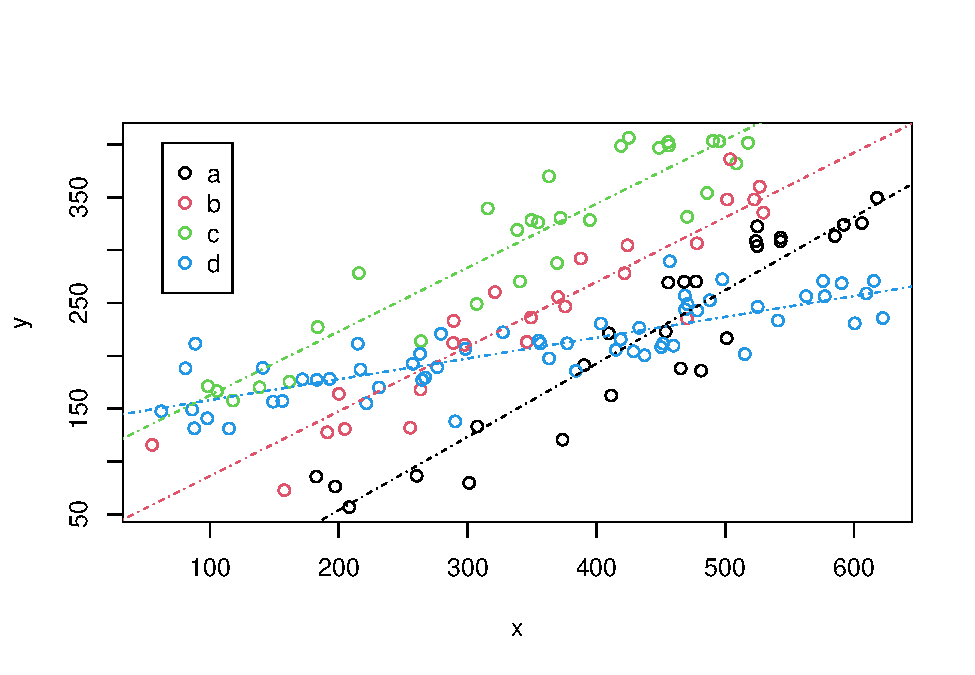
\includegraphics{ECOMODbook_files/figure-latex/a7.15-1.pdf}

Naturally, now the lines do not have the same slope, and we can compare all these in a single plot. This plot is really messy, as it includes the pooled regression (the thick black line), the regressions fitted to independent data sets, one for each museum (the solid lines), and the regressions resulting from the model with museum as a factor covariate (dotted-dashed lines).

\begin{Shaded}
\begin{Highlighting}[]
\CommentTok{\#plot all the data}
\FunctionTok{plot}\NormalTok{(y}\SpecialCharTok{\textasciitilde{}}\NormalTok{x,}\AttributeTok{col=}\FunctionTok{as.numeric}\NormalTok{(}\FunctionTok{as.factor}\NormalTok{(z)),}\AttributeTok{data=}\NormalTok{data4lines,}\AttributeTok{pch=}\DecValTok{1}\NormalTok{)}
\CommentTok{\#completely independet regression lines}
\FunctionTok{abline}\NormalTok{(}\FunctionTok{lm}\NormalTok{(y}\SpecialCharTok{\textasciitilde{}}\NormalTok{x,}\AttributeTok{data=}\NormalTok{data4lines[data4lines}\SpecialCharTok{$}\NormalTok{z}\SpecialCharTok{==}\StringTok{"a"}\NormalTok{,]),}\AttributeTok{col=}\DecValTok{1}\NormalTok{,}\AttributeTok{lty=}\DecValTok{4}\NormalTok{)}
\FunctionTok{abline}\NormalTok{(}\FunctionTok{lm}\NormalTok{(y}\SpecialCharTok{\textasciitilde{}}\NormalTok{x,}\AttributeTok{data=}\NormalTok{data4lines[data4lines}\SpecialCharTok{$}\NormalTok{z}\SpecialCharTok{==}\StringTok{"b"}\NormalTok{,]),}\AttributeTok{col=}\DecValTok{2}\NormalTok{,}\AttributeTok{lty=}\DecValTok{4}\NormalTok{)}
\FunctionTok{abline}\NormalTok{(}\FunctionTok{lm}\NormalTok{(y}\SpecialCharTok{\textasciitilde{}}\NormalTok{x,}\AttributeTok{data=}\NormalTok{data4lines[data4lines}\SpecialCharTok{$}\NormalTok{z}\SpecialCharTok{==}\StringTok{"c"}\NormalTok{,]),}\AttributeTok{col=}\DecValTok{3}\NormalTok{,}\AttributeTok{lty=}\DecValTok{4}\NormalTok{)}
\FunctionTok{abline}\NormalTok{(}\FunctionTok{lm}\NormalTok{(y}\SpecialCharTok{\textasciitilde{}}\NormalTok{x,}\AttributeTok{data=}\NormalTok{data4lines[data4lines}\SpecialCharTok{$}\NormalTok{z}\SpecialCharTok{==}\StringTok{"d"}\NormalTok{,]),}\AttributeTok{col=}\DecValTok{4}\NormalTok{,}\AttributeTok{lty=}\DecValTok{4}\NormalTok{)}
\CommentTok{\#these are the wrong lines... why?}
\FunctionTok{abline}\NormalTok{(lmlinesG,}\AttributeTok{lwd=}\DecValTok{3}\NormalTok{,}\AttributeTok{lty=}\DecValTok{2}\NormalTok{)}
\FunctionTok{abline}\NormalTok{(lmlines}\SpecialCharTok{$}\NormalTok{coefficients[}\DecValTok{1}\NormalTok{],lmlines}\SpecialCharTok{$}\NormalTok{coefficients[}\DecValTok{2}\NormalTok{],}\AttributeTok{col=}\DecValTok{1}\NormalTok{)}
\FunctionTok{abline}\NormalTok{(lmlines}\SpecialCharTok{$}\NormalTok{coefficients[}\DecValTok{1}\NormalTok{]}\SpecialCharTok{+}\NormalTok{lmlines}\SpecialCharTok{$}\NormalTok{coefficients[}\DecValTok{3}\NormalTok{],lmlines}\SpecialCharTok{$}\NormalTok{coefficients[}\DecValTok{2}\NormalTok{],}\AttributeTok{col=}\DecValTok{2}\NormalTok{)}
\FunctionTok{abline}\NormalTok{(lmlines}\SpecialCharTok{$}\NormalTok{coefficients[}\DecValTok{1}\NormalTok{]}\SpecialCharTok{+}\NormalTok{lmlines}\SpecialCharTok{$}\NormalTok{coefficients[}\DecValTok{4}\NormalTok{],lmlines}\SpecialCharTok{$}\NormalTok{coefficients[}\DecValTok{2}\NormalTok{],}\AttributeTok{col=}\DecValTok{3}\NormalTok{)}
\FunctionTok{abline}\NormalTok{(lmlines}\SpecialCharTok{$}\NormalTok{coefficients[}\DecValTok{1}\NormalTok{]}\SpecialCharTok{+}\NormalTok{lmlines}\SpecialCharTok{$}\NormalTok{coefficients[}\DecValTok{5}\NormalTok{],lmlines}\SpecialCharTok{$}\NormalTok{coefficients[}\DecValTok{2}\NormalTok{],}\AttributeTok{col=}\DecValTok{4}\NormalTok{)}
\end{Highlighting}
\end{Shaded}

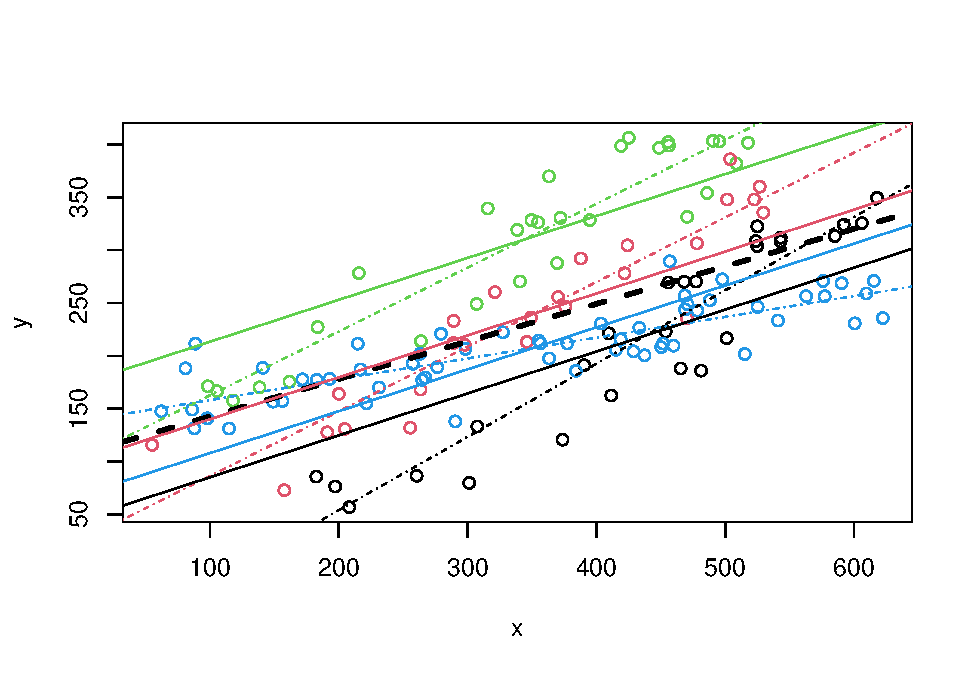
\includegraphics{ECOMODbook_files/figure-latex/a7.16-1.pdf}

But what is the best model to describe the data? That is a mistery that will remain to unfold. For that we will need and additional complication in a regression model: interactions.

But note 1 thing to begin with. The pooled model uses just 2 parameters, one slope and one intercept. The independent lines use 8 parameters, 4 slopes and 4 intercepts, one line for each museum. And the single model with \texttt{lenght} and \texttt{museum} uses 5 parameters, the intercept, the slope for \texttt{length}, and 3 parameters associated with the \(k-1=3\) levels of \texttt{museum} (remember, one level of each factor is absorbed by the regression intercept).

So the choice of what is best might be not straightforward. While we created the data by hand, we do not know the true model! Choosing the best model requires choosing between models with different complexity, i.e.~different number of parameters. We will need a parsimonious model, one that describes the data well, but with a number of parameters that is not too high for the available data. That will also require selection criteria.

Stay tuned for the next episodes on our regression saga!

\hypertarget{aula8}{%
\chapter{Class 8 20 10 2020 - t-test and ANOVA are just linear models}\label{aula8}}

The objective of this chapter is to explore different regression models and to see how they relate to statistical procedures one might not at first associate with a regression, when in fact, they are just special cases of a standard linear models, i.e.~special cases of regression models.

\hypertarget{the-t-test}{%
\section{The t-test}\label{the-t-test}}

While we did not do the t-test in class, this is useful because it allows you to see how a simple t-test is just a linear model too, and acts as a building block for the next examples. The two sample t-test allows us to test the null hypothesis that two samples have the same mean.

Create some data

\begin{Shaded}
\begin{Highlighting}[]
\CommentTok{\#Making up a t{-}test}
\CommentTok{\#making sure everyone gets the same results}
\FunctionTok{set.seed}\NormalTok{(}\DecValTok{980}\NormalTok{)}
\end{Highlighting}
\end{Shaded}

Then we define the sample size and the number of treatments

\begin{Shaded}
\begin{Highlighting}[]
\CommentTok{\#define sample size}
\NormalTok{n}\OtherTok{=}\DecValTok{100}
\CommentTok{\#define treatments}
\NormalTok{tr}\OtherTok{=}\FunctionTok{c}\NormalTok{(}\StringTok{"a"}\NormalTok{,}\StringTok{"b"}\NormalTok{)}
\CommentTok{\#how many treatments {-} 2 for a t test}
\NormalTok{ntr}\OtherTok{=}\FunctionTok{length}\NormalTok{(tr)}
\CommentTok{\#balanced design}
\NormalTok{n.by.tr}\OtherTok{=}\NormalTok{n}\SpecialCharTok{/}\NormalTok{ntr}
\end{Highlighting}
\end{Shaded}

Now, we can simulate some data. First, the treatments

\begin{Shaded}
\begin{Highlighting}[]
\NormalTok{type}\OtherTok{=}\FunctionTok{as.factor}\NormalTok{(}\FunctionTok{rep}\NormalTok{(tr,}\AttributeTok{each=}\NormalTok{n.by.tr))}
\NormalTok{cores}\OtherTok{=}\FunctionTok{rep}\NormalTok{(}\DecValTok{1}\SpecialCharTok{:}\NormalTok{ntr,}\AttributeTok{each=}\NormalTok{n.by.tr)}
\end{Highlighting}
\end{Shaded}

Then we define the means by treatment - note that they are different, so the null hypothesis in the t-test, that the mean of a is equal to the mean of b, is known to be false in this case.

\begin{Shaded}
\begin{Highlighting}[]
\CommentTok{\#define 4 means}
\NormalTok{ms}\OtherTok{=}\FunctionTok{c}\NormalTok{(}\DecValTok{3}\NormalTok{,}\DecValTok{4}\NormalTok{)}
\end{Highlighting}
\end{Shaded}

Then, the key part, the response variable, with a different mean by treatment. Note the use of the \texttt{ifelse} function, which evaluates its first argument and then assigns the value of its second argument if the first is true or the value of the second if its first argument is false. An example

\begin{Shaded}
\begin{Highlighting}[]
\FunctionTok{ifelse}\NormalTok{(}\DecValTok{3}\SpecialCharTok{\textgreater{}}\DecValTok{4}\NormalTok{,}\DecValTok{55}\NormalTok{,}\DecValTok{77}\NormalTok{)}
\end{Highlighting}
\end{Shaded}

\begin{verbatim}
## [1] 77
\end{verbatim}

\begin{Shaded}
\begin{Highlighting}[]
\FunctionTok{ifelse}\NormalTok{(}\DecValTok{3}\SpecialCharTok{\textless{}}\DecValTok{4}\NormalTok{,}\DecValTok{55}\NormalTok{,}\DecValTok{77}\NormalTok{)}
\end{Highlighting}
\end{Shaded}

\begin{verbatim}
## [1] 55
\end{verbatim}

So now, generate the response data

\begin{Shaded}
\begin{Highlighting}[]
\NormalTok{ys}\OtherTok{=}\FunctionTok{ifelse}\NormalTok{(type}\SpecialCharTok{==}\StringTok{"a"}\NormalTok{,ms[}\DecValTok{1}\NormalTok{],ms[}\DecValTok{2}\NormalTok{])}\SpecialCharTok{+}\FunctionTok{rnorm}\NormalTok{(n,}\DecValTok{0}\NormalTok{,}\FloatTok{1.5}\NormalTok{)}
\end{Highlighting}
\end{Shaded}

Look at the data

\begin{Shaded}
\begin{Highlighting}[]
\FunctionTok{plot}\NormalTok{(ys}\SpecialCharTok{\textasciitilde{}}\NormalTok{type)}
\end{Highlighting}
\end{Shaded}

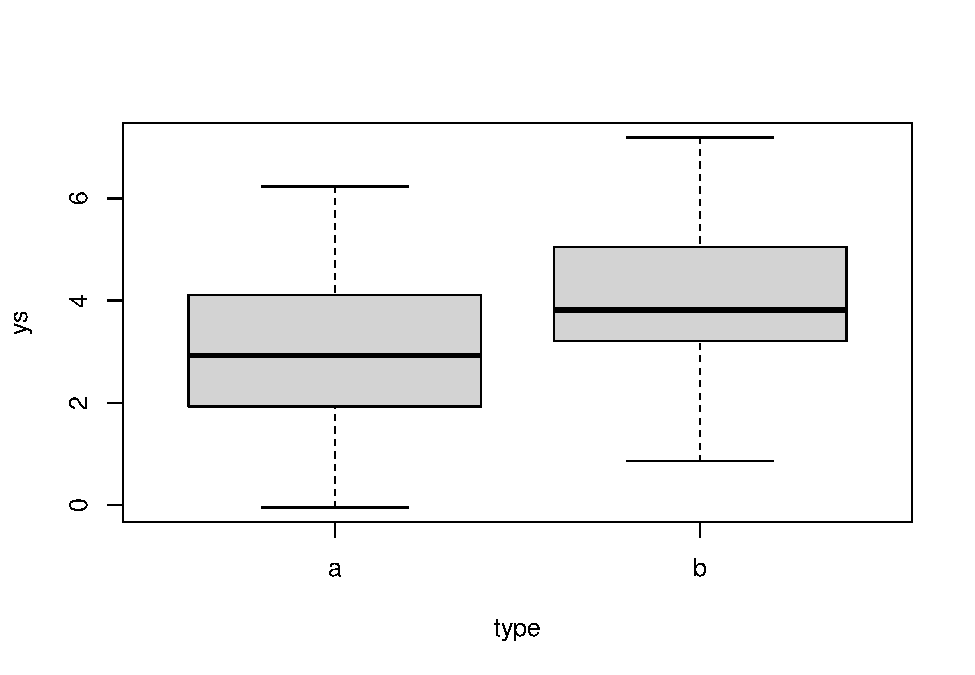
\includegraphics{ECOMODbook_files/figure-latex/a8.7-1.pdf}

Now, we can run the usual t-test

\begin{Shaded}
\begin{Highlighting}[]
\FunctionTok{t.test}\NormalTok{(ys}\SpecialCharTok{\textasciitilde{}}\NormalTok{type)}
\end{Highlighting}
\end{Shaded}

\begin{verbatim}
## 
##  Welch Two Sample t-test
## 
## data:  ys by type
## t = -2.8043, df = 97.475, p-value = 0.006087
## alternative hypothesis: true difference in means is not equal to 0
## 95 percent confidence interval:
##  -1.4263293 -0.2441277
## sample estimates:
## mean in group a mean in group b 
##        3.106656        3.941884
\end{verbatim}

and now we can do it the linear regression way

\begin{Shaded}
\begin{Highlighting}[]
\NormalTok{lm0}\OtherTok{=}\FunctionTok{lm}\NormalTok{(ys}\SpecialCharTok{\textasciitilde{}}\NormalTok{type)}
\FunctionTok{summary}\NormalTok{(lm0)}
\end{Highlighting}
\end{Shaded}

\begin{verbatim}
## 
## Call:
## lm(formula = ys ~ type)
## 
## Residuals:
##     Min      1Q  Median      3Q     Max 
## -3.1489 -0.9131 -0.1315  1.0295  3.2450 
## 
## Coefficients:
##             Estimate Std. Error t value Pr(>|t|)    
## (Intercept)   3.1067     0.2106  14.751  < 2e-16 ***
## typeb         0.8352     0.2978   2.804  0.00608 ** 
## ---
## Signif. codes:  0 '***' 0.001 '**' 0.01 '*' 0.05 '.' 0.1 ' ' 1
## 
## Residual standard error: 1.489 on 98 degrees of freedom
## Multiple R-squared:  0.07428,    Adjusted R-squared:  0.06484 
## F-statistic: 7.864 on 1 and 98 DF,  p-value: 0.006081
\end{verbatim}

and as you can see, we get the same result for the test statistic. It is the same thing! And we can naturally get the estimated means per group. The mean for a is just the intercept of the model. To get the mean of the group b we add the mean of group b to the intercept, as

\begin{Shaded}
\begin{Highlighting}[]
\CommentTok{\#mean of ys under treatment a}
\FunctionTok{summary}\NormalTok{(lm0)}\SpecialCharTok{$}\NormalTok{coefficients[}\DecValTok{1}\NormalTok{]}
\end{Highlighting}
\end{Shaded}

\begin{verbatim}
## [1] 3.106656
\end{verbatim}

\begin{Shaded}
\begin{Highlighting}[]
\CommentTok{\#mean of ys under treatment b}
\FunctionTok{summary}\NormalTok{(lm0)}\SpecialCharTok{$}\NormalTok{coefficients[}\DecValTok{1}\NormalTok{]}\SpecialCharTok{+}\NormalTok{lm0}\SpecialCharTok{$}\NormalTok{coefficients[}\DecValTok{2}\NormalTok{]}
\end{Highlighting}
\end{Shaded}

\begin{verbatim}
##    typeb 
## 3.941884
\end{verbatim}

This is required because in a linear model, all the other parameters associated with levels of a factor will be compared to a reference value, that of the intercept, which happens to be the mean under treatment a. Below you will see more examples of this.

Note we were able to detect the null was false, but this was because we had a decent sample size compared to the variance of the measurements and the magnitude of the true effect (the difference of the means). If we keep the sample size constant but we increase the noise or decrease the magnitude of the difference, we might not get the same result, and make a type II error!

\begin{Shaded}
\begin{Highlighting}[]
\CommentTok{\#define 2 means}
\NormalTok{ms}\OtherTok{=}\FunctionTok{c}\NormalTok{(}\DecValTok{3}\NormalTok{,}\DecValTok{4}\NormalTok{)}
\CommentTok{\#increase the variance of the process}
\NormalTok{ys}\OtherTok{=}\FunctionTok{ifelse}\NormalTok{(type}\SpecialCharTok{==}\StringTok{"a"}\NormalTok{,ms[}\DecValTok{1}\NormalTok{],ms[}\DecValTok{2}\NormalTok{])}\SpecialCharTok{+}\FunctionTok{rnorm}\NormalTok{(n,}\DecValTok{0}\NormalTok{,}\DecValTok{5}\NormalTok{)}
\end{Highlighting}
\end{Shaded}

Look at the data, we can see much more variation

\begin{Shaded}
\begin{Highlighting}[]
\FunctionTok{plot}\NormalTok{(ys}\SpecialCharTok{\textasciitilde{}}\NormalTok{type)}
\end{Highlighting}
\end{Shaded}

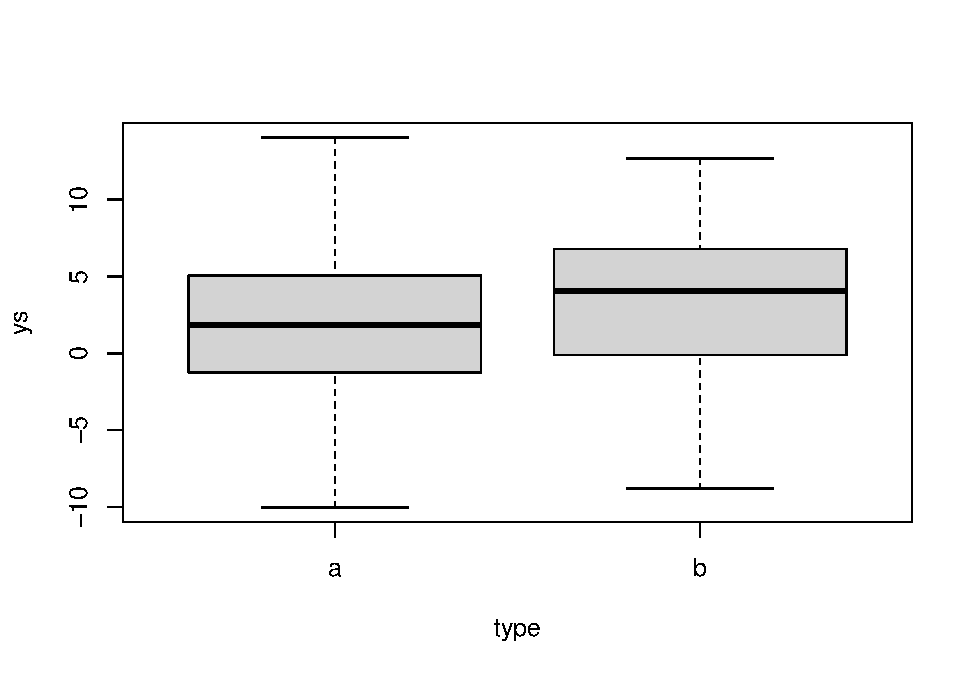
\includegraphics{ECOMODbook_files/figure-latex/a8.12-1.pdf}

Now, we can run the usual t-test

\begin{Shaded}
\begin{Highlighting}[]
\FunctionTok{t.test}\NormalTok{(ys}\SpecialCharTok{\textasciitilde{}}\NormalTok{type)}
\end{Highlighting}
\end{Shaded}

\begin{verbatim}
## 
##  Welch Two Sample t-test
## 
## data:  ys by type
## t = -1.3609, df = 97.949, p-value = 0.1767
## alternative hypothesis: true difference in means is not equal to 0
## 95 percent confidence interval:
##  -3.2822693  0.6118174
## sample estimates:
## mean in group a mean in group b 
##        2.024963        3.360189
\end{verbatim}

and now we can do it the linear regression way

\begin{Shaded}
\begin{Highlighting}[]
\NormalTok{lm0}\OtherTok{=}\FunctionTok{lm}\NormalTok{(ys}\SpecialCharTok{\textasciitilde{}}\NormalTok{type)}
\FunctionTok{summary}\NormalTok{(lm0)}
\end{Highlighting}
\end{Shaded}

\begin{verbatim}
## 
## Call:
## lm(formula = ys ~ type)
## 
## Residuals:
##      Min       1Q   Median       3Q      Max 
## -12.1746  -3.2719   0.2527   3.0578  12.0085 
## 
## Coefficients:
##             Estimate Std. Error t value Pr(>|t|)   
## (Intercept)   2.0250     0.6938   2.919  0.00436 **
## typeb         1.3352     0.9811   1.361  0.17667   
## ---
## Signif. codes:  0 '***' 0.001 '**' 0.01 '*' 0.05 '.' 0.1 ' ' 1
## 
## Residual standard error: 4.906 on 98 degrees of freedom
## Multiple R-squared:  0.01855,    Adjusted R-squared:  0.008533 
## F-statistic: 1.852 on 1 and 98 DF,  p-value: 0.1767
\end{verbatim}

and as you can see, we get the same result for the test statistic, but now with a non significant test.

The same would have happened if we decreased the true difference, while keeping the original magnitude of the error

\begin{Shaded}
\begin{Highlighting}[]
\CommentTok{\#define 2 means}
\NormalTok{ms}\OtherTok{=}\FunctionTok{c}\NormalTok{(}\DecValTok{3}\NormalTok{,}\FloatTok{3.1}\NormalTok{)}
\CommentTok{\#increase the variance of the process}
\NormalTok{ys}\OtherTok{=}\FunctionTok{ifelse}\NormalTok{(type}\SpecialCharTok{==}\StringTok{"a"}\NormalTok{,ms[}\DecValTok{1}\NormalTok{],ms[}\DecValTok{2}\NormalTok{])}\SpecialCharTok{+}\FunctionTok{rnorm}\NormalTok{(n,}\DecValTok{0}\NormalTok{,}\FloatTok{1.5}\NormalTok{)}
\end{Highlighting}
\end{Shaded}

Look at the data, we can see again lower variation, but the difference across treatments is very small (so, hard to detect!)

\begin{Shaded}
\begin{Highlighting}[]
\FunctionTok{plot}\NormalTok{(ys}\SpecialCharTok{\textasciitilde{}}\NormalTok{type)}
\end{Highlighting}
\end{Shaded}

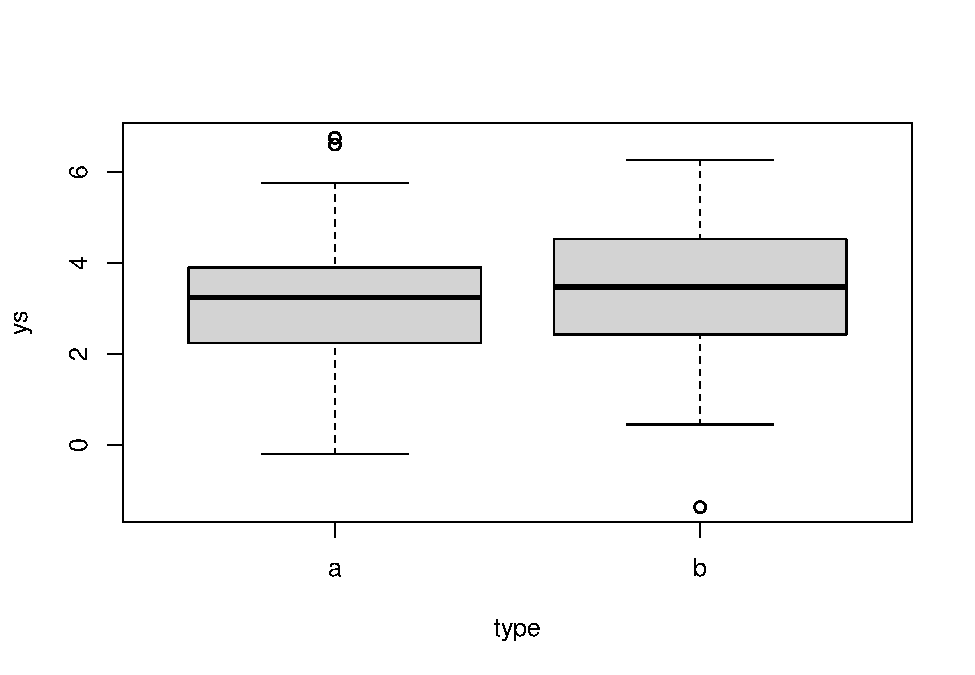
\includegraphics{ECOMODbook_files/figure-latex/a8.16-1.pdf}

Now, we can run the usual t-test

\begin{Shaded}
\begin{Highlighting}[]
\FunctionTok{t.test}\NormalTok{(ys}\SpecialCharTok{\textasciitilde{}}\NormalTok{type)}
\end{Highlighting}
\end{Shaded}

\begin{verbatim}
## 
##  Welch Two Sample t-test
## 
## data:  ys by type
## t = -0.7994, df = 97.455, p-value = 0.426
## alternative hypothesis: true difference in means is not equal to 0
## 95 percent confidence interval:
##  -0.8149517  0.3469402
## sample estimates:
## mean in group a mean in group b 
##        3.158868        3.392874
\end{verbatim}

and now we can do it the linear regression way

\begin{Shaded}
\begin{Highlighting}[]
\NormalTok{lm0}\OtherTok{=}\FunctionTok{lm}\NormalTok{(ys}\SpecialCharTok{\textasciitilde{}}\NormalTok{type)}
\FunctionTok{summary}\NormalTok{(lm0)}
\end{Highlighting}
\end{Shaded}

\begin{verbatim}
## 
## Call:
## lm(formula = ys ~ type)
## 
## Residuals:
##     Min      1Q  Median      3Q     Max 
## -4.7661 -0.9318  0.0812  0.9087  3.5981 
## 
## Coefficients:
##             Estimate Std. Error t value Pr(>|t|)    
## (Intercept)   3.1589     0.2070  15.261   <2e-16 ***
## typeb         0.2340     0.2927   0.799    0.426    
## ---
## Signif. codes:  0 '***' 0.001 '**' 0.01 '*' 0.05 '.' 0.1 ' ' 1
## 
## Residual standard error: 1.464 on 98 degrees of freedom
## Multiple R-squared:  0.006479,   Adjusted R-squared:  -0.003659 
## F-statistic: 0.639 on 1 and 98 DF,  p-value: 0.426
\end{verbatim}

\hypertarget{anova}{%
\section{ANOVA}\label{anova}}

We move on with perhaps the most famous example of a statistical test/procedure, the ANOVA. An ANOVA is nothing but a linear model, where we have a continuous response variable, which we want to explain as a function of a factor (with several levels, or treatments).

There is a slight difference in the way we can code the dummy variables that might be worth to explore (this relates to contrasts, but perhaps beyond what I want to let the students know? cf.~\url{https://www.theanalysisfactor.com/why-anova-and-linear-regression-are-the-same-analysis/}).

Here we simulate a data set, beginning by making sure everyone gets the same results by using \texttt{set.seed}

\begin{Shaded}
\begin{Highlighting}[]
\CommentTok{\#Making up an ANOVA}
\CommentTok{\#An ANOVA}
\CommentTok{\#making sure everyone gets the same results}
\FunctionTok{set.seed}\NormalTok{(}\DecValTok{12345}\NormalTok{)}
\end{Highlighting}
\end{Shaded}

Then we define the sample size and the number of treatments

\begin{Shaded}
\begin{Highlighting}[]
\CommentTok{\#define sample size}
\NormalTok{n}\OtherTok{=}\DecValTok{2000}
\CommentTok{\#define treatments}
\NormalTok{tr}\OtherTok{=}\FunctionTok{c}\NormalTok{(}\StringTok{"a"}\NormalTok{,}\StringTok{"b"}\NormalTok{,}\StringTok{"c"}\NormalTok{,}\StringTok{"d"}\NormalTok{)}
\CommentTok{\#how many treatments}
\NormalTok{ntr}\OtherTok{=}\FunctionTok{length}\NormalTok{(tr)}
\CommentTok{\#balanced design}
\NormalTok{n.by.tr}\OtherTok{=}\NormalTok{n}\SpecialCharTok{/}\NormalTok{ntr}
\end{Highlighting}
\end{Shaded}

now, we can simulate some data. First, the treatments, but we also generate a independent variable that is not really used for now (\texttt{xs}).

\begin{Shaded}
\begin{Highlighting}[]
\CommentTok{\#generate data}
\NormalTok{xs}\OtherTok{=}\FunctionTok{runif}\NormalTok{(n,}\DecValTok{10}\NormalTok{,}\DecValTok{20}\NormalTok{)}
\NormalTok{type}\OtherTok{=}\FunctionTok{as.factor}\NormalTok{(}\FunctionTok{rep}\NormalTok{(tr,}\AttributeTok{each=}\NormalTok{n.by.tr))}
\CommentTok{\#if I wanted to recode the levels such that c was the baseline}
\CommentTok{\#type=factor(type,levels = c("c","a","b","d"))}
\CommentTok{\#get colors for plotting}
\NormalTok{cores}\OtherTok{=}\FunctionTok{rep}\NormalTok{(}\DecValTok{1}\SpecialCharTok{:}\NormalTok{ntr,}\AttributeTok{each=}\NormalTok{n.by.tr)}
\end{Highlighting}
\end{Shaded}

Then we define the means by treatment - note that they are different, so the null hypothesis in an ANOVA, that all the means are the same, is false.

\begin{Shaded}
\begin{Highlighting}[]
\CommentTok{\#define 4 means}
\NormalTok{ms}\OtherTok{=}\FunctionTok{c}\NormalTok{(}\DecValTok{3}\NormalTok{,}\DecValTok{5}\NormalTok{,}\DecValTok{6}\NormalTok{,}\DecValTok{2}\NormalTok{)}
\end{Highlighting}
\end{Shaded}

Then, the key part, the response variable, with a different mean by treatment. Note the use of the \texttt{ifelse} function, which evaluates its first argument and then assigns the value of its second argument if the first is true or the value of the second if its first argument is false. An example

\begin{Shaded}
\begin{Highlighting}[]
\FunctionTok{ifelse}\NormalTok{(}\DecValTok{3}\SpecialCharTok{\textgreater{}}\DecValTok{4}\NormalTok{,}\DecValTok{55}\NormalTok{,}\DecValTok{77}\NormalTok{)}
\end{Highlighting}
\end{Shaded}

\begin{verbatim}
## [1] 77
\end{verbatim}

\begin{Shaded}
\begin{Highlighting}[]
\FunctionTok{ifelse}\NormalTok{(}\DecValTok{3}\SpecialCharTok{\textless{}}\DecValTok{4}\NormalTok{,}\DecValTok{55}\NormalTok{,}\DecValTok{77}\NormalTok{)}
\end{Highlighting}
\end{Shaded}

\begin{verbatim}
## [1] 55
\end{verbatim}

Note these can be used nested, leading to possible multiple outcomes, and I use that below to define 4 different means depending on the treatment of the observation

\begin{Shaded}
\begin{Highlighting}[]
\FunctionTok{ifelse}\NormalTok{(}\DecValTok{3}\SpecialCharTok{\textless{}}\DecValTok{4}\NormalTok{,}\DecValTok{55}\NormalTok{,}\FunctionTok{ifelse}\NormalTok{(}\DecValTok{3}\SpecialCharTok{\textgreater{}}\DecValTok{2}\NormalTok{,}\DecValTok{55}\NormalTok{,}\DecValTok{68}\NormalTok{))}
\end{Highlighting}
\end{Shaded}

\begin{verbatim}
## [1] 55
\end{verbatim}

\begin{Shaded}
\begin{Highlighting}[]
\FunctionTok{ifelse}\NormalTok{(}\DecValTok{3}\SpecialCharTok{\textgreater{}}\DecValTok{4}\NormalTok{,}\DecValTok{55}\NormalTok{,}\FunctionTok{ifelse}\NormalTok{(}\DecValTok{3}\SpecialCharTok{\textgreater{}}\DecValTok{2}\NormalTok{,}\DecValTok{666}\NormalTok{,}\DecValTok{68}\NormalTok{))}
\end{Highlighting}
\end{Shaded}

\begin{verbatim}
## [1] 666
\end{verbatim}

\begin{Shaded}
\begin{Highlighting}[]
\FunctionTok{ifelse}\NormalTok{(}\DecValTok{3}\SpecialCharTok{\textgreater{}}\DecValTok{4}\NormalTok{,}\DecValTok{55}\NormalTok{,}\FunctionTok{ifelse}\NormalTok{(}\DecValTok{3}\SpecialCharTok{\textless{}}\DecValTok{2}\NormalTok{,}\DecValTok{666}\NormalTok{,}\DecValTok{68}\NormalTok{))}
\end{Highlighting}
\end{Shaded}

\begin{verbatim}
## [1] 68
\end{verbatim}

So now, generate the data

\begin{Shaded}
\begin{Highlighting}[]
\CommentTok{\#ys, not a function of the xs!!!}
\NormalTok{ys}\OtherTok{=}\FunctionTok{ifelse}\NormalTok{(type}\SpecialCharTok{==}\StringTok{"a"}\NormalTok{,ms[}\DecValTok{1}\NormalTok{],}\FunctionTok{ifelse}\NormalTok{(type}\SpecialCharTok{==}\StringTok{"b"}\NormalTok{,ms[}\DecValTok{2}\NormalTok{],}\FunctionTok{ifelse}\NormalTok{(type}\SpecialCharTok{==}\StringTok{"c"}\NormalTok{,ms[}\DecValTok{3}\NormalTok{],ms[}\DecValTok{4}\NormalTok{])))}\SpecialCharTok{+}\FunctionTok{rnorm}\NormalTok{(n,}\DecValTok{0}\NormalTok{,}\DecValTok{3}\NormalTok{)}
\end{Highlighting}
\end{Shaded}

We can actually look at the simulated data

\begin{Shaded}
\begin{Highlighting}[]
\FunctionTok{par}\NormalTok{(}\AttributeTok{mfrow=}\FunctionTok{c}\NormalTok{(}\DecValTok{1}\NormalTok{,}\DecValTok{1}\NormalTok{),}\AttributeTok{mar=}\FunctionTok{c}\NormalTok{(}\DecValTok{4}\NormalTok{,}\DecValTok{4}\NormalTok{,}\FloatTok{0.5}\NormalTok{,}\FloatTok{0.5}\NormalTok{))}
\FunctionTok{plot}\NormalTok{(ys}\SpecialCharTok{\textasciitilde{}}\NormalTok{type,}\AttributeTok{col=}\DecValTok{1}\SpecialCharTok{:}\DecValTok{4}\NormalTok{)}
\end{Highlighting}
\end{Shaded}

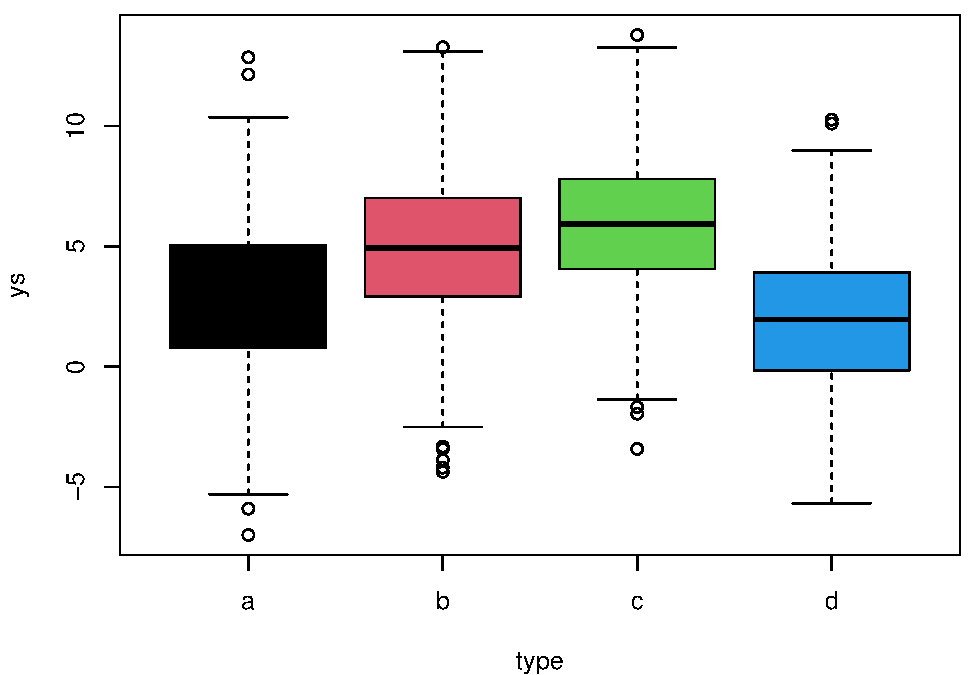
\includegraphics{ECOMODbook_files/figure-latex/a8.26-1.pdf}

\begin{Shaded}
\begin{Highlighting}[]
\CommentTok{\#abline(h=ms,col=1:4)}
\end{Highlighting}
\end{Shaded}

finally, we can implement the linear model and look at its summary

\begin{Shaded}
\begin{Highlighting}[]
\NormalTok{lm.anova}\OtherTok{=}\FunctionTok{lm}\NormalTok{(ys}\SpecialCharTok{\textasciitilde{}}\NormalTok{type)}
\FunctionTok{summary}\NormalTok{(lm.anova)}
\end{Highlighting}
\end{Shaded}

\begin{verbatim}
## 
## Call:
## lm(formula = ys ~ type)
## 
## Residuals:
##     Min      1Q  Median      3Q     Max 
## -9.8735 -2.0115  0.0301  2.0208  9.9976 
## 
## Coefficients:
##             Estimate Std. Error t value Pr(>|t|)    
## (Intercept)   2.8694     0.1319  21.753  < 2e-16 ***
## typeb         2.0788     0.1865  11.143  < 2e-16 ***
## typec         2.9806     0.1865  15.978  < 2e-16 ***
## typed        -0.8726     0.1865  -4.678 3.09e-06 ***
## ---
## Signif. codes:  0 '***' 0.001 '**' 0.01 '*' 0.05 '.' 0.1 ' ' 1
## 
## Residual standard error: 2.95 on 1996 degrees of freedom
## Multiple R-squared:  0.2163, Adjusted R-squared:  0.2151 
## F-statistic: 183.6 on 3 and 1996 DF,  p-value: < 2.2e-16
\end{verbatim}

note that, again, we can manipulate any sub-components of the created objects

\begin{Shaded}
\begin{Highlighting}[]
\CommentTok{\#see the parameters}
\NormalTok{lm.anova}\SpecialCharTok{$}\NormalTok{coefficients}
\end{Highlighting}
\end{Shaded}

\begin{verbatim}
## (Intercept)       typeb       typec       typed 
##   2.8694412   2.0787628   2.9806367  -0.8726428
\end{verbatim}

\begin{Shaded}
\begin{Highlighting}[]
\CommentTok{\#see the third parameter}
\NormalTok{lm.anova}\SpecialCharTok{$}\NormalTok{coefficients[}\DecValTok{3}\NormalTok{]}
\end{Highlighting}
\end{Shaded}

\begin{verbatim}
##    typec 
## 2.980637
\end{verbatim}

Not surprisingly, because the means were different and we had a large sample size, everything is highly significant. Note that the ANOVA test is actually presented in the regression output, and that is the corresponding F-test

\begin{Shaded}
\begin{Highlighting}[]
\FunctionTok{summary}\NormalTok{(lm.anova)}\SpecialCharTok{$}\NormalTok{fstatistic}
\end{Highlighting}
\end{Shaded}

\begin{verbatim}
##     value     numdf     dendf 
##  183.6156    3.0000 1996.0000
\end{verbatim}

and we can use the F distribution to calculate the corresponding P-value (note that is already in the output above)

\begin{Shaded}
\begin{Highlighting}[]
\NormalTok{ftest}\OtherTok{=}\FunctionTok{summary}\NormalTok{(lm.anova)}\SpecialCharTok{$}\NormalTok{fstatistic[}\DecValTok{1}\NormalTok{]}
\NormalTok{df1}\OtherTok{=}\FunctionTok{summary}\NormalTok{(lm.anova)}\SpecialCharTok{$}\NormalTok{fstatistic[}\DecValTok{2}\NormalTok{]}
\NormalTok{df2}\OtherTok{=}\FunctionTok{summary}\NormalTok{(lm.anova)}\SpecialCharTok{$}\NormalTok{fstatistic[}\DecValTok{3}\NormalTok{]}
\FunctionTok{pt}\NormalTok{(ftest,df1,df2)}
\end{Highlighting}
\end{Shaded}

\begin{verbatim}
##         value 
## 1.402786e-131
\end{verbatim}

OK, this is actually the exact value, while above the value was reported as just a small value (\textless{} 2.2 \(\times\) 10\(^{-16}\)), but it is the same value, believe me!

Finally, to show (by example) this is just what the ANOVA does, we have the NAOVA itself

\begin{Shaded}
\begin{Highlighting}[]
\FunctionTok{summary}\NormalTok{(}\FunctionTok{aov}\NormalTok{(lm.anova))}
\end{Highlighting}
\end{Shaded}

\begin{verbatim}
##               Df Sum Sq Mean Sq F value Pr(>F)    
## type           3   4792  1597.5   183.6 <2e-16 ***
## Residuals   1996  17365     8.7                   
## ---
## Signif. codes:  0 '***' 0.001 '**' 0.01 '*' 0.05 '.' 0.1 ' ' 1
\end{verbatim}

where everything is the same (test statistic, degrees of freedom and p-values).

Conclusion: an ANOVA is just a special case of a linear model, one where we have a continuous response variable and a factor explanatory covariate. In fact, a two way ANOVA is just the extension where we have a continuous response variable and 2 factor explanatory covariates, and, you guessed it, a three way ANOVA means we have a continuous response variable and a 3 factor explanatory covariates.

Just to finish up this example, we could now plot the true means per treatment, the estimated means per treatment

\begin{Shaded}
\begin{Highlighting}[]
\FunctionTok{par}\NormalTok{(}\AttributeTok{mfrow=}\FunctionTok{c}\NormalTok{(}\DecValTok{1}\NormalTok{,}\DecValTok{1}\NormalTok{),}\AttributeTok{mar=}\FunctionTok{c}\NormalTok{(}\DecValTok{4}\NormalTok{,}\DecValTok{4}\NormalTok{,}\FloatTok{0.5}\NormalTok{,}\FloatTok{0.5}\NormalTok{))}
\FunctionTok{plot}\NormalTok{(}\FunctionTok{as.numeric}\NormalTok{(type),ys,}\AttributeTok{col=}\FunctionTok{as.numeric}\NormalTok{(type),}\AttributeTok{xlab=}\StringTok{"Treatment"}\NormalTok{,}\AttributeTok{xaxt=}\StringTok{"n"}\NormalTok{)}
\FunctionTok{axis}\NormalTok{(}\DecValTok{1}\NormalTok{,}\AttributeTok{at=}\DecValTok{1}\SpecialCharTok{:}\DecValTok{4}\NormalTok{,letters[}\DecValTok{1}\SpecialCharTok{:}\DecValTok{4}\NormalTok{])}
\CommentTok{\#plot the estimated line for type a}
\FunctionTok{abline}\NormalTok{(}\AttributeTok{h=}\NormalTok{lm.anova}\SpecialCharTok{$}\NormalTok{coefficients[}\DecValTok{1}\NormalTok{],}\AttributeTok{lwd=}\DecValTok{3}\NormalTok{,}\AttributeTok{col=}\DecValTok{1}\NormalTok{)}
\CommentTok{\#plot the mean line for type a}
\FunctionTok{abline}\NormalTok{(}\AttributeTok{h=}\FunctionTok{mean}\NormalTok{(ys[type}\SpecialCharTok{==}\StringTok{"a"}\NormalTok{]),}\AttributeTok{lwd=}\DecValTok{1}\NormalTok{,}\AttributeTok{col=}\DecValTok{1}\NormalTok{,}\AttributeTok{lty=}\DecValTok{2}\NormalTok{)}
\CommentTok{\#plot the real mean for type a}
\FunctionTok{abline}\NormalTok{(}\AttributeTok{h=}\NormalTok{ms[}\DecValTok{1}\NormalTok{],}\AttributeTok{lwd=}\DecValTok{2}\NormalTok{,}\AttributeTok{col=}\DecValTok{1}\NormalTok{,}\AttributeTok{lty=}\DecValTok{3}\NormalTok{)}
\CommentTok{\#and now for the other types}
\FunctionTok{abline}\NormalTok{(}\AttributeTok{h=}\NormalTok{lm.anova}\SpecialCharTok{$}\NormalTok{coefficients[}\DecValTok{1}\NormalTok{]}\SpecialCharTok{+}\NormalTok{lm.anova}\SpecialCharTok{$}\NormalTok{coefficients[}\DecValTok{2}\NormalTok{],}\AttributeTok{lwd=}\DecValTok{3}\NormalTok{,}\AttributeTok{col=}\DecValTok{2}\NormalTok{)}
\FunctionTok{abline}\NormalTok{(}\AttributeTok{h=}\FunctionTok{mean}\NormalTok{(ys[type}\SpecialCharTok{==}\StringTok{"b"}\NormalTok{]),}\AttributeTok{lwd=}\DecValTok{1}\NormalTok{,}\AttributeTok{col=}\DecValTok{2}\NormalTok{,}\AttributeTok{lty=}\DecValTok{2}\NormalTok{)}
\CommentTok{\#plot the real mean for type b}
\FunctionTok{abline}\NormalTok{(}\AttributeTok{h=}\NormalTok{ms[}\DecValTok{2}\NormalTok{],}\AttributeTok{lwd=}\DecValTok{2}\NormalTok{,}\AttributeTok{col=}\DecValTok{2}\NormalTok{,}\AttributeTok{lty=}\DecValTok{3}\NormalTok{)}
\FunctionTok{abline}\NormalTok{(}\AttributeTok{h=}\NormalTok{lm.anova}\SpecialCharTok{$}\NormalTok{coefficients[}\DecValTok{1}\NormalTok{]}\SpecialCharTok{+}\NormalTok{lm.anova}\SpecialCharTok{$}\NormalTok{coefficients[}\DecValTok{3}\NormalTok{],}\AttributeTok{lwd=}\DecValTok{3}\NormalTok{,}\AttributeTok{col=}\DecValTok{3}\NormalTok{)}
\FunctionTok{abline}\NormalTok{(}\AttributeTok{h=}\FunctionTok{mean}\NormalTok{(ys[type}\SpecialCharTok{==}\StringTok{"c"}\NormalTok{]),}\AttributeTok{lwd=}\DecValTok{1}\NormalTok{,}\AttributeTok{col=}\DecValTok{3}\NormalTok{,}\AttributeTok{lty=}\DecValTok{2}\NormalTok{)}
\CommentTok{\#plot the real mean for type c}
\FunctionTok{abline}\NormalTok{(}\AttributeTok{h=}\NormalTok{ms[}\DecValTok{3}\NormalTok{],}\AttributeTok{lwd=}\DecValTok{2}\NormalTok{,}\AttributeTok{col=}\DecValTok{3}\NormalTok{,}\AttributeTok{lty=}\DecValTok{3}\NormalTok{)}
\FunctionTok{abline}\NormalTok{(}\AttributeTok{h=}\NormalTok{lm.anova}\SpecialCharTok{$}\NormalTok{coefficients[}\DecValTok{1}\NormalTok{]}\SpecialCharTok{+}\NormalTok{lm.anova}\SpecialCharTok{$}\NormalTok{coefficients[}\DecValTok{4}\NormalTok{],}\AttributeTok{lwd=}\DecValTok{3}\NormalTok{,}\AttributeTok{col=}\DecValTok{4}\NormalTok{)}
\FunctionTok{abline}\NormalTok{(}\AttributeTok{h=}\FunctionTok{mean}\NormalTok{(ys[type}\SpecialCharTok{==}\StringTok{"d"}\NormalTok{]),}\AttributeTok{lwd=}\DecValTok{1}\NormalTok{,}\AttributeTok{col=}\DecValTok{4}\NormalTok{,}\AttributeTok{lty=}\DecValTok{2}\NormalTok{)}
\CommentTok{\#plot the real mean for type a}
\FunctionTok{abline}\NormalTok{(}\AttributeTok{h=}\NormalTok{ms[}\DecValTok{4}\NormalTok{],}\AttributeTok{lwd=}\DecValTok{2}\NormalTok{,}\AttributeTok{col=}\DecValTok{4}\NormalTok{,}\AttributeTok{lty=}\DecValTok{3}\NormalTok{)}
\FunctionTok{legend}\NormalTok{(}\StringTok{"topright"}\NormalTok{,}\FunctionTok{c}\NormalTok{(}\StringTok{"Estimated"}\NormalTok{,}\StringTok{"Mean of data"}\NormalTok{,}\StringTok{"True"}\NormalTok{),}\AttributeTok{lwd=}\FunctionTok{c}\NormalTok{(}\DecValTok{4}\NormalTok{,}\DecValTok{1}\NormalTok{,}\DecValTok{2}\NormalTok{),}\AttributeTok{lty=}\FunctionTok{c}\NormalTok{(}\DecValTok{1}\NormalTok{,}\DecValTok{3}\NormalTok{,}\DecValTok{2}\NormalTok{),}\AttributeTok{inset=}\FloatTok{0.03}\NormalTok{)}
\end{Highlighting}
\end{Shaded}

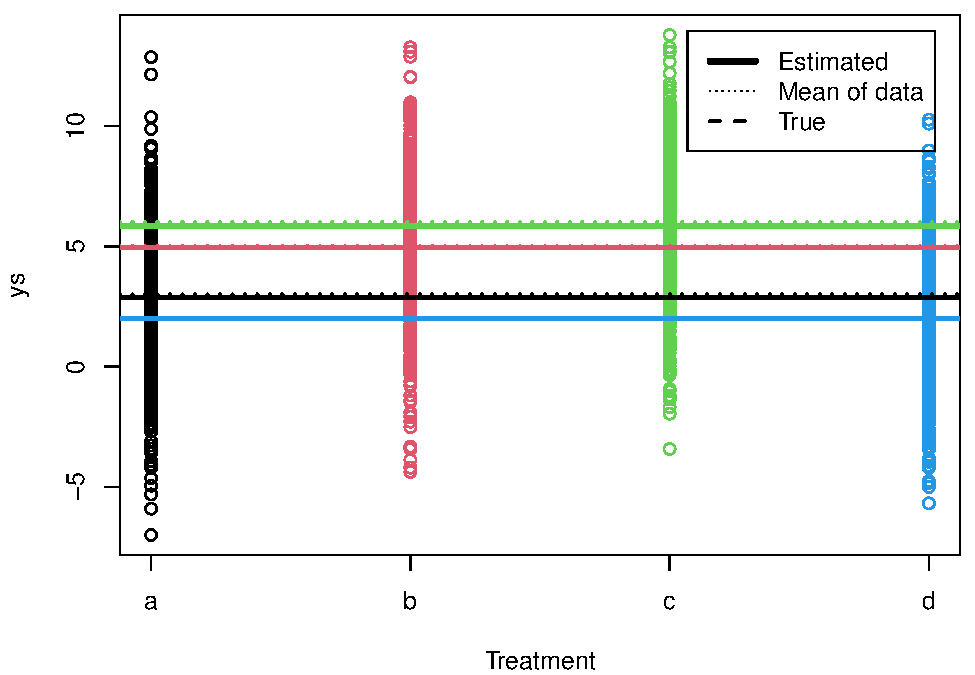
\includegraphics{ECOMODbook_files/figure-latex/a8.32-1.pdf}

It's not easy to see because these overlap (large sample size, high precision) but the estimated means are really close to the real means. It's a bit easier to see if we separate in 4 plots and zoom in on the mean of each treatment, but still the blue lines are all on top of each other, since the mean value was estimated real close to truth (truth=2, estimated = 1.9967984).

\begin{Shaded}
\begin{Highlighting}[]
\CommentTok{\#see this in 4 plots, less blur}
\FunctionTok{par}\NormalTok{(}\AttributeTok{mfrow=}\FunctionTok{c}\NormalTok{(}\DecValTok{2}\NormalTok{,}\DecValTok{2}\NormalTok{),}\AttributeTok{mar=}\FunctionTok{c}\NormalTok{(}\DecValTok{4}\NormalTok{,}\DecValTok{4}\NormalTok{,}\FloatTok{0.5}\NormalTok{,}\FloatTok{0.5}\NormalTok{))}
\FunctionTok{plot}\NormalTok{(}\FunctionTok{as.numeric}\NormalTok{(type),ys,}\AttributeTok{col=}\FunctionTok{as.numeric}\NormalTok{(type),}\AttributeTok{xlab=}\StringTok{"Treatment"}\NormalTok{,}\AttributeTok{xaxt=}\StringTok{"n"}\NormalTok{,}\AttributeTok{ylim=}\FunctionTok{mean}\NormalTok{(ys[type}\SpecialCharTok{==}\StringTok{"a"}\NormalTok{])}\SpecialCharTok{+}\FunctionTok{c}\NormalTok{(}\SpecialCharTok{{-}}\FloatTok{0.5}\NormalTok{,}\FloatTok{0.5}\NormalTok{))}
\FunctionTok{axis}\NormalTok{(}\DecValTok{1}\NormalTok{,}\AttributeTok{at=}\DecValTok{1}\SpecialCharTok{:}\DecValTok{4}\NormalTok{,letters[}\DecValTok{1}\SpecialCharTok{:}\DecValTok{4}\NormalTok{])}
\CommentTok{\#plot the estimated line for type a}
\FunctionTok{abline}\NormalTok{(}\AttributeTok{h=}\NormalTok{lm.anova}\SpecialCharTok{$}\NormalTok{coefficients[}\DecValTok{1}\NormalTok{],}\AttributeTok{lwd=}\DecValTok{3}\NormalTok{,}\AttributeTok{col=}\DecValTok{1}\NormalTok{)}
\CommentTok{\#plot the mean line for type a}
\FunctionTok{abline}\NormalTok{(}\AttributeTok{h=}\FunctionTok{mean}\NormalTok{(ys[type}\SpecialCharTok{==}\StringTok{"a"}\NormalTok{]),}\AttributeTok{lwd=}\DecValTok{1}\NormalTok{,}\AttributeTok{col=}\DecValTok{1}\NormalTok{,}\AttributeTok{lty=}\DecValTok{2}\NormalTok{)}
\CommentTok{\#plot the real mean for type a}
\FunctionTok{abline}\NormalTok{(}\AttributeTok{h=}\NormalTok{ms[}\DecValTok{1}\NormalTok{],}\AttributeTok{lwd=}\DecValTok{2}\NormalTok{,}\AttributeTok{col=}\DecValTok{1}\NormalTok{,}\AttributeTok{lty=}\DecValTok{3}\NormalTok{)}
\CommentTok{\#and now for the other types}
\FunctionTok{plot}\NormalTok{(}\FunctionTok{as.numeric}\NormalTok{(type),ys,}\AttributeTok{col=}\FunctionTok{as.numeric}\NormalTok{(type),}\AttributeTok{xlab=}\StringTok{"Treatment"}\NormalTok{,}\AttributeTok{xaxt=}\StringTok{"n"}\NormalTok{,}\AttributeTok{ylim=}\FunctionTok{mean}\NormalTok{(ys[type}\SpecialCharTok{==}\StringTok{"b"}\NormalTok{])}\SpecialCharTok{+}\FunctionTok{c}\NormalTok{(}\SpecialCharTok{{-}}\FloatTok{0.5}\NormalTok{,}\FloatTok{0.5}\NormalTok{))}
\FunctionTok{axis}\NormalTok{(}\DecValTok{1}\NormalTok{,}\AttributeTok{at=}\DecValTok{1}\SpecialCharTok{:}\DecValTok{4}\NormalTok{,letters[}\DecValTok{1}\SpecialCharTok{:}\DecValTok{4}\NormalTok{])}
\FunctionTok{abline}\NormalTok{(}\AttributeTok{h=}\NormalTok{lm.anova}\SpecialCharTok{$}\NormalTok{coefficients[}\DecValTok{1}\NormalTok{]}\SpecialCharTok{+}\NormalTok{lm.anova}\SpecialCharTok{$}\NormalTok{coefficients[}\DecValTok{2}\NormalTok{],}\AttributeTok{lwd=}\DecValTok{3}\NormalTok{,}\AttributeTok{col=}\DecValTok{2}\NormalTok{)}
\FunctionTok{abline}\NormalTok{(}\AttributeTok{h=}\FunctionTok{mean}\NormalTok{(ys[type}\SpecialCharTok{==}\StringTok{"b"}\NormalTok{]),}\AttributeTok{lwd=}\DecValTok{1}\NormalTok{,}\AttributeTok{col=}\DecValTok{2}\NormalTok{,}\AttributeTok{lty=}\DecValTok{2}\NormalTok{)}
\CommentTok{\#plot the real mean for type b}
\FunctionTok{abline}\NormalTok{(}\AttributeTok{h=}\NormalTok{ms[}\DecValTok{2}\NormalTok{],}\AttributeTok{lwd=}\DecValTok{2}\NormalTok{,}\AttributeTok{col=}\DecValTok{2}\NormalTok{,}\AttributeTok{lty=}\DecValTok{3}\NormalTok{)}
\FunctionTok{plot}\NormalTok{(}\FunctionTok{as.numeric}\NormalTok{(type),ys,}\AttributeTok{col=}\FunctionTok{as.numeric}\NormalTok{(type),}\AttributeTok{xlab=}\StringTok{"Treatment"}\NormalTok{,}\AttributeTok{xaxt=}\StringTok{"n"}\NormalTok{,}\AttributeTok{ylim=}\FunctionTok{mean}\NormalTok{(ys[type}\SpecialCharTok{==}\StringTok{"c"}\NormalTok{])}\SpecialCharTok{+}\FunctionTok{c}\NormalTok{(}\SpecialCharTok{{-}}\FloatTok{0.5}\NormalTok{,}\FloatTok{0.5}\NormalTok{))}
\FunctionTok{axis}\NormalTok{(}\DecValTok{1}\NormalTok{,}\AttributeTok{at=}\DecValTok{1}\SpecialCharTok{:}\DecValTok{4}\NormalTok{,letters[}\DecValTok{1}\SpecialCharTok{:}\DecValTok{4}\NormalTok{])}
\FunctionTok{abline}\NormalTok{(}\AttributeTok{h=}\NormalTok{lm.anova}\SpecialCharTok{$}\NormalTok{coefficients[}\DecValTok{1}\NormalTok{]}\SpecialCharTok{+}\NormalTok{lm.anova}\SpecialCharTok{$}\NormalTok{coefficients[}\DecValTok{3}\NormalTok{],}\AttributeTok{lwd=}\DecValTok{3}\NormalTok{,}\AttributeTok{col=}\DecValTok{3}\NormalTok{)}
\FunctionTok{abline}\NormalTok{(}\AttributeTok{h=}\FunctionTok{mean}\NormalTok{(ys[type}\SpecialCharTok{==}\StringTok{"c"}\NormalTok{]),}\AttributeTok{lwd=}\DecValTok{1}\NormalTok{,}\AttributeTok{col=}\DecValTok{3}\NormalTok{,}\AttributeTok{lty=}\DecValTok{2}\NormalTok{)}
\CommentTok{\#plot the real mean for type c}
\FunctionTok{abline}\NormalTok{(}\AttributeTok{h=}\NormalTok{ms[}\DecValTok{3}\NormalTok{],}\AttributeTok{lwd=}\DecValTok{2}\NormalTok{,}\AttributeTok{col=}\DecValTok{3}\NormalTok{,}\AttributeTok{lty=}\DecValTok{3}\NormalTok{)}
\FunctionTok{plot}\NormalTok{(}\FunctionTok{as.numeric}\NormalTok{(type),ys,}\AttributeTok{col=}\FunctionTok{as.numeric}\NormalTok{(type),}\AttributeTok{xlab=}\StringTok{"Treatment"}\NormalTok{,}\AttributeTok{xaxt=}\StringTok{"n"}\NormalTok{,}\AttributeTok{ylim=}\FunctionTok{mean}\NormalTok{(ys[type}\SpecialCharTok{==}\StringTok{"d"}\NormalTok{])}\SpecialCharTok{+}\FunctionTok{c}\NormalTok{(}\SpecialCharTok{{-}}\FloatTok{0.5}\NormalTok{,}\FloatTok{0.5}\NormalTok{))}
\FunctionTok{axis}\NormalTok{(}\DecValTok{1}\NormalTok{,}\AttributeTok{at=}\DecValTok{1}\SpecialCharTok{:}\DecValTok{4}\NormalTok{,letters[}\DecValTok{1}\SpecialCharTok{:}\DecValTok{4}\NormalTok{])}
\FunctionTok{abline}\NormalTok{(}\AttributeTok{h=}\NormalTok{lm.anova}\SpecialCharTok{$}\NormalTok{coefficients[}\DecValTok{1}\NormalTok{]}\SpecialCharTok{+}\NormalTok{lm.anova}\SpecialCharTok{$}\NormalTok{coefficients[}\DecValTok{4}\NormalTok{],}\AttributeTok{lwd=}\DecValTok{3}\NormalTok{,}\AttributeTok{col=}\DecValTok{4}\NormalTok{)}
\FunctionTok{abline}\NormalTok{(}\AttributeTok{h=}\FunctionTok{mean}\NormalTok{(ys[type}\SpecialCharTok{==}\StringTok{"d"}\NormalTok{]),}\AttributeTok{lwd=}\DecValTok{1}\NormalTok{,}\AttributeTok{col=}\DecValTok{4}\NormalTok{,}\AttributeTok{lty=}\DecValTok{2}\NormalTok{)}
\CommentTok{\#plot the real mean for type a}
\FunctionTok{abline}\NormalTok{(}\AttributeTok{h=}\NormalTok{ms[}\DecValTok{4}\NormalTok{],}\AttributeTok{lwd=}\DecValTok{2}\NormalTok{,}\AttributeTok{col=}\DecValTok{4}\NormalTok{,}\AttributeTok{lty=}\DecValTok{3}\NormalTok{)}
\end{Highlighting}
\end{Shaded}

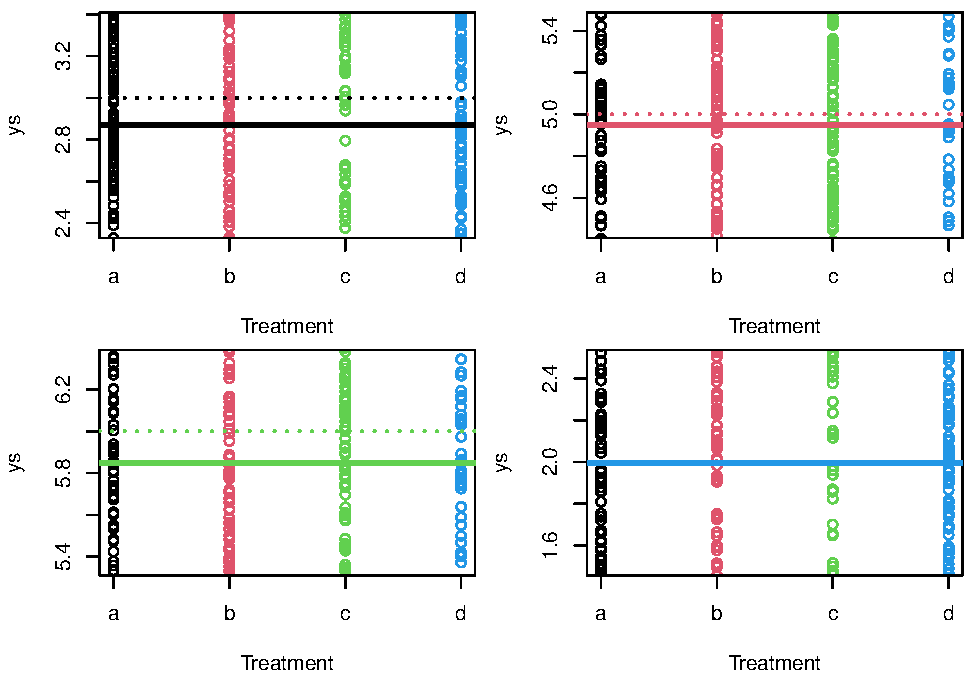
\includegraphics{ECOMODbook_files/figure-latex/a8.33-1.pdf}

\begin{Shaded}
\begin{Highlighting}[]
\CommentTok{\#legend("bottomright",c("Estimated","Mean of data","True"),lwd=c(4,1,2),lty=c(1,3,2),inset=0.05)}
\end{Highlighting}
\end{Shaded}

Now we can check how we can obtain the estimated means from the actual parameters of the regression model (yes, that is what the regression does, it calculates the expected mean of the response, conditional on the treatment).

This is the estimated mean per treatment, using function \texttt{tapply} (very useful function to get any statistics over a variable, inside groups defined by a second variable, here the treatment)

\begin{Shaded}
\begin{Highlighting}[]
\FunctionTok{tapply}\NormalTok{(}\AttributeTok{X=}\NormalTok{ys,}\AttributeTok{INDEX=}\NormalTok{type,}\AttributeTok{FUN=}\NormalTok{mean)}
\end{Highlighting}
\end{Shaded}

\begin{verbatim}
##        a        b        c        d 
## 2.869441 4.948204 5.850078 1.996798
\end{verbatim}

and checking these are obtained from the regression coefficients.
An important note. When you fit models with factors (like here), the intercept term will correspond to the mean of the reference level of the factor(s). Hence, to get the other means, you always have to sum the parameter of the corresponding level to the intercept. So we do it below

\begin{Shaded}
\begin{Highlighting}[]
\CommentTok{\#check ANOVA is just computing the mean in each group}
\NormalTok{lm.anova}\SpecialCharTok{$}\NormalTok{coefficients[}\DecValTok{1}\NormalTok{]}
\end{Highlighting}
\end{Shaded}

\begin{verbatim}
## (Intercept) 
##    2.869441
\end{verbatim}

\begin{Shaded}
\begin{Highlighting}[]
\NormalTok{lm.anova}\SpecialCharTok{$}\NormalTok{coefficients[}\DecValTok{1}\NormalTok{]}\SpecialCharTok{+}\NormalTok{lm.anova}\SpecialCharTok{$}\NormalTok{coefficients[}\DecValTok{2}\NormalTok{]}
\end{Highlighting}
\end{Shaded}

\begin{verbatim}
## (Intercept) 
##    4.948204
\end{verbatim}

\begin{Shaded}
\begin{Highlighting}[]
\NormalTok{lm.anova}\SpecialCharTok{$}\NormalTok{coefficients[}\DecValTok{1}\NormalTok{]}\SpecialCharTok{+}\NormalTok{lm.anova}\SpecialCharTok{$}\NormalTok{coefficients[}\DecValTok{3}\NormalTok{]}
\end{Highlighting}
\end{Shaded}

\begin{verbatim}
## (Intercept) 
##    5.850078
\end{verbatim}

\begin{Shaded}
\begin{Highlighting}[]
\NormalTok{lm.anova}\SpecialCharTok{$}\NormalTok{coefficients[}\DecValTok{1}\NormalTok{]}\SpecialCharTok{+}\NormalTok{lm.anova}\SpecialCharTok{$}\NormalTok{coefficients[}\DecValTok{4}\NormalTok{]}
\end{Highlighting}
\end{Shaded}

\begin{verbatim}
## (Intercept) 
##    1.996798
\end{verbatim}

and we can see these are exactly the same values.

\hypertarget{a-two-way-anova-and-beyhond-ex-task-do-it-yourself}{%
\section{A two way ANOVA, and beyhond (ex Task: do it yourself!)}\label{a-two-way-anova-and-beyhond-ex-task-do-it-yourself}}

The dataset \texttt{penguins} in the package \texttt{palmerpenguins} is very useful to illustrate ANOVA's. It includes body size measurements (bill length and depth, flipper length and body mass) by sex for adult foraging penguins near Palmer Station, Antarctica, for 3 different islands.

I found out about this data in this twitter post by Trevor Branch (@~TrevorABranch, \url{https://twitter.com/TrevorABranch/status/1333844966632607745}). This dataset was made as an R package by Allison Horst (yes, the same person that makes the amazing R abd RStudio related artwork that we used before, \url{https://www.allisonhorst.com/}). Here we brighten up our book with Allison's artwork again, for a reminder that the residuals of the ANOVA should be approximately Gaussian, with constant variance! If they are not Gaussian, you might more elaborate models, like a GLM, say.

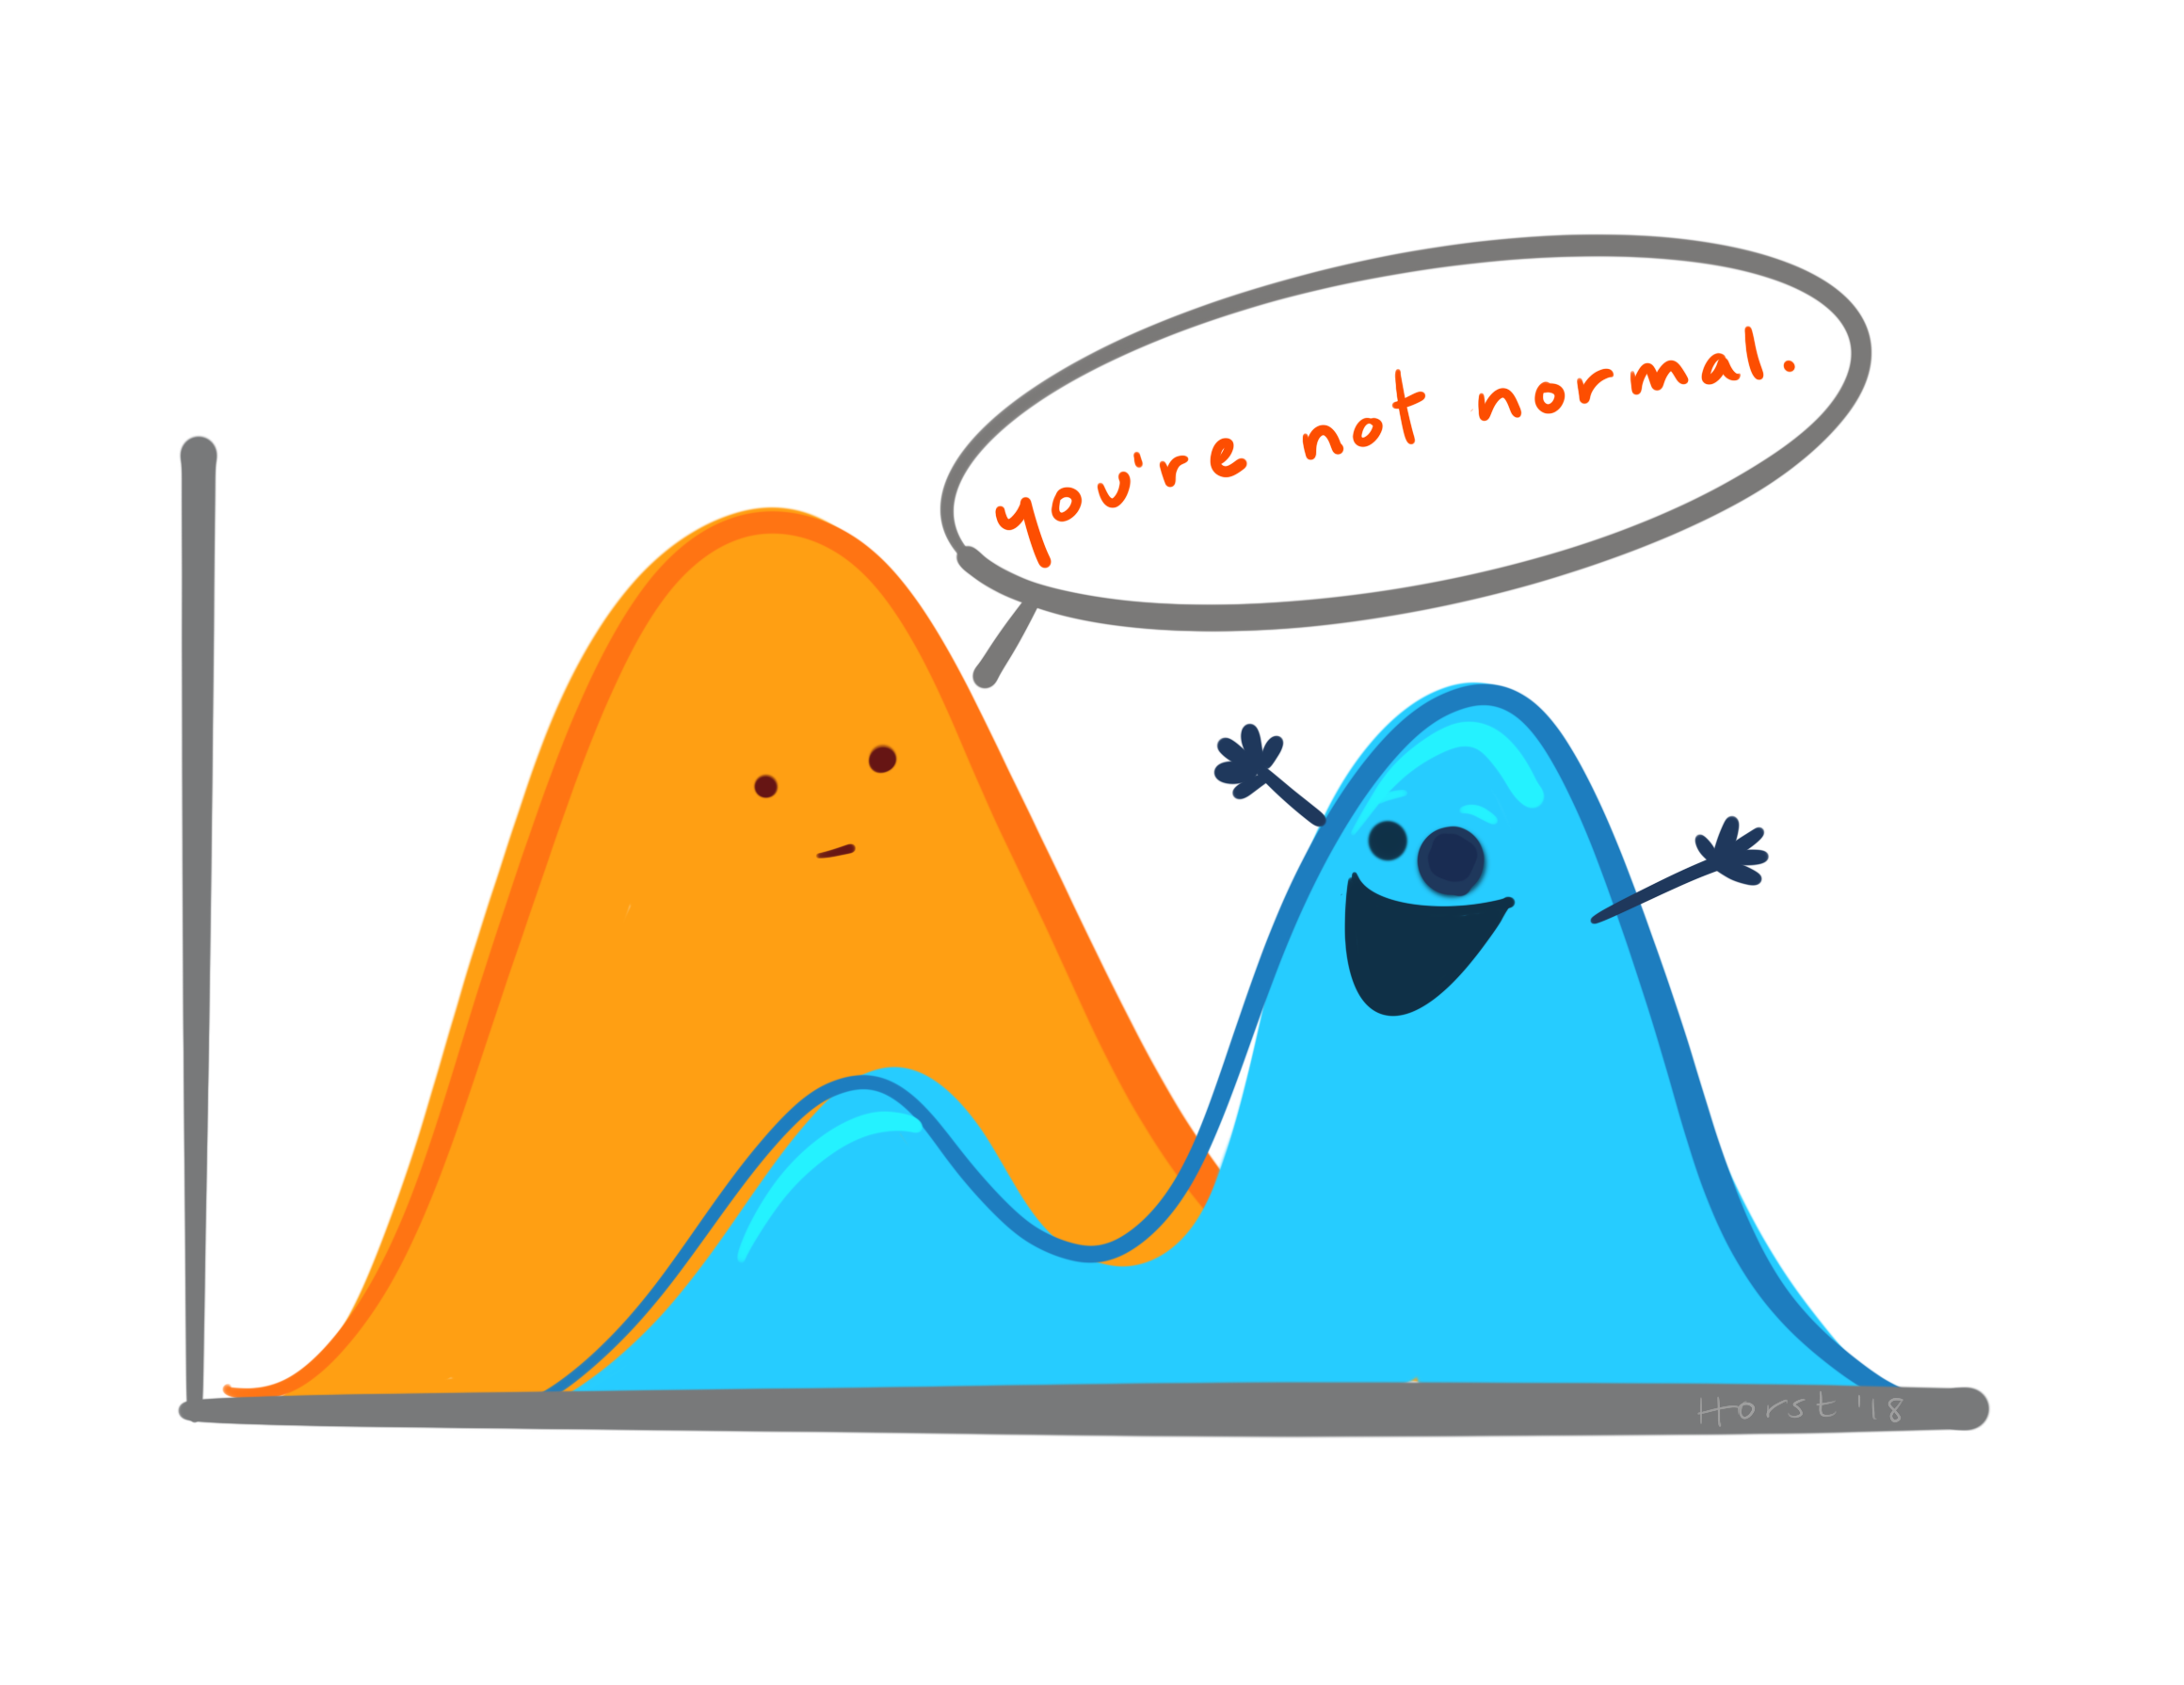
\includegraphics{extfiles/not_normal.png}
Looking at the dataset in question, explore the two way ANOVA as a linear model, and then, we move way past beyhond that into a bit of how to interpret a multiple regression output.

\begin{Shaded}
\begin{Highlighting}[]
\FunctionTok{library}\NormalTok{(palmerpenguins)}
\FunctionTok{data}\NormalTok{(penguins)}
\end{Highlighting}
\end{Shaded}

Just to make it easier, we remove some records of penguins for which there is no sex. Always think about what might be the impact of removing data, but here we assume these are missing at random and hence would not bias inferences.

\begin{Shaded}
\begin{Highlighting}[]
\NormalTok{penguins}\OtherTok{\textless{}{-}}\NormalTok{penguins[}\SpecialCharTok{!}\FunctionTok{is.na}\NormalTok{(penguins}\SpecialCharTok{$}\NormalTok{sex),]}
\end{Highlighting}
\end{Shaded}

Lets check how many animals we have in each treatment (a treatment is jargon for the level of a factor covariate, or for a combination of levels in a factorial experiment).

\begin{Shaded}
\begin{Highlighting}[]
\FunctionTok{barplot}\NormalTok{(}\FunctionTok{with}\NormalTok{(penguins,}\FunctionTok{table}\NormalTok{(species,sex)))}
\end{Highlighting}
\end{Shaded}

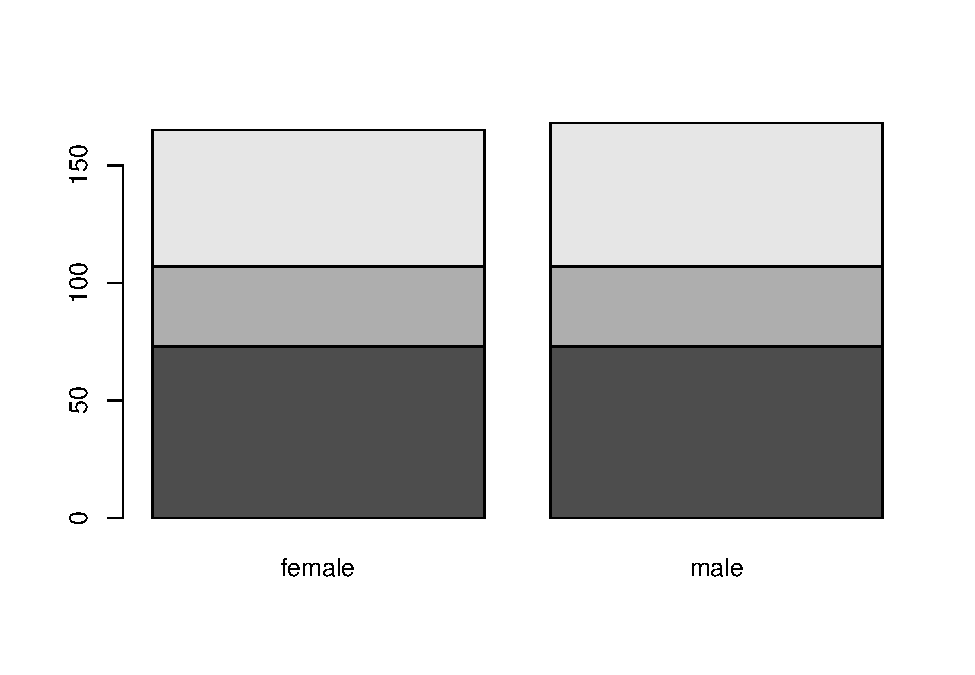
\includegraphics{ECOMODbook_files/figure-latex/unnamed-chunk-3-1.pdf}

Perhaps surprisingly given this is observational data, the number of animals per island is balanced across sexes. On the other hane, more animals are coming from Adelie than from Gentoo, and Chinstrap presents overall a lower number of animals.

Imagine you are researcher wanting to explain how the flipper length depends on the animal's sex and species. Given that we have a response variable as a function of two factor covariates, an interaction plot comes in handy. This visualization, available through function \texttt{interaction.plot}, allows us to see how the data varies as a function of the level of multiple factors. The interaction plot below illustrates the data of the flipper length (in millimeters) as a function of sex and species.

\begin{verbatim}
with(penguins,interaction.plot(x.factor=species,trace.factor=sex,response=flipper_length_mm,ylab="Flipper length (mm)"))
\end{verbatim}

Looking at this plot tells us little about whether the two variables are significant or not, because we do not really have a notion of variability associated with it. But it does seem like size might be different by sex and by species, with males being apparently larger than females, and animals from Gentoo being considerably larger than those from Adelie and Chinstrap. There do not seem to be strong interactions, but whether possible interactions are present or not remains to be seen. If the lines are parallel then there are by definition no interactions, i.e., the effect of a variable does not depend on the effect of another, and vice versa. The problem is that looking at the plot alone tells us nothing about how much those lines deviate from being parallel or not.

Note that strictly the interaction plot needs to be interpreted with care because the lines are not in any way supposed to be taken as if the relationship is continuous. The slope of the lines dows give us however an idea about the differences between the different treatments.

We can actually look at the observation in each of the treatments (i.e.~combinations of sex and island)

\begin{Shaded}
\begin{Highlighting}[]
\FunctionTok{par}\NormalTok{(}\AttributeTok{mar=}\FunctionTok{c}\NormalTok{(}\DecValTok{10}\NormalTok{,}\DecValTok{4}\NormalTok{,}\DecValTok{0}\NormalTok{,}\DecValTok{0}\NormalTok{))}
\FunctionTok{with}\NormalTok{(penguins,}\FunctionTok{boxplot}\NormalTok{(flipper\_length\_mm }\SpecialCharTok{\textasciitilde{}}\NormalTok{ species }\SpecialCharTok{+}\NormalTok{ sex,}\AttributeTok{las=}\DecValTok{2}\NormalTok{,}\AttributeTok{xlab=}\StringTok{""}\NormalTok{,}\AttributeTok{col=}\FunctionTok{c}\NormalTok{(}\DecValTok{1}\NormalTok{,}\DecValTok{2}\NormalTok{,}\DecValTok{3}\NormalTok{,}\DecValTok{1}\NormalTok{,}\DecValTok{2}\NormalTok{,}\DecValTok{3}\NormalTok{)))}
\end{Highlighting}
\end{Shaded}

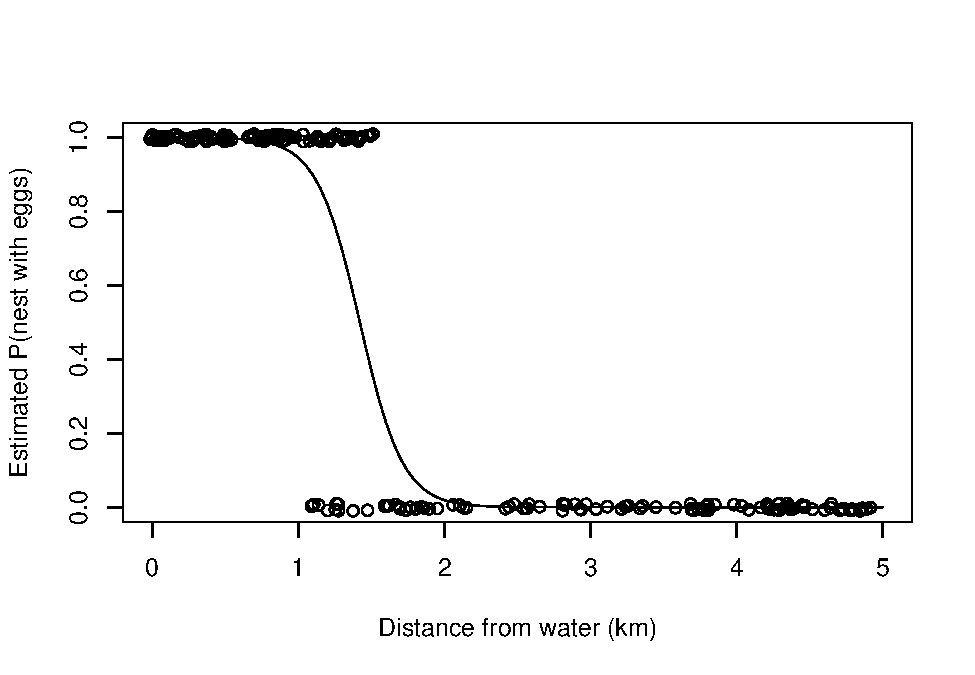
\includegraphics{ECOMODbook_files/figure-latex/unnamed-chunk-4-1.pdf}

This plot does allow us to see the variability of the data, and it is likely that several terms will be considered statistically significant. We can implement the linear model that corresponds to the two way ANOVA to formally test that

\begin{Shaded}
\begin{Highlighting}[]
\NormalTok{lm2wayANOVA}\OtherTok{\textless{}{-}}\FunctionTok{lm}\NormalTok{(flipper\_length\_mm}\SpecialCharTok{\textasciitilde{}}\NormalTok{species}\SpecialCharTok{+}\NormalTok{sex,}\AttributeTok{data=}\NormalTok{penguins)}
\FunctionTok{summary}\NormalTok{(lm2wayANOVA)}
\end{Highlighting}
\end{Shaded}

\begin{verbatim}
## 
## Call:
## lm(formula = flipper_length_mm ~ species + sex, data = penguins)
## 
## Residuals:
##      Min       1Q   Median       3Q      Max 
## -15.5278  -3.7239   0.2761   3.4722  16.4722 
## 
## Coefficients:
##                  Estimate Std. Error t value Pr(>|t|)    
## (Intercept)      186.6777     0.5684 328.437  < 2e-16 ***
## speciesChinstrap   5.7208     0.8407   6.805 4.79e-11 ***
## speciesGentoo     27.0462     0.7072  38.243  < 2e-16 ***
## sexmale            6.8502     0.6276  10.914  < 2e-16 ***
## ---
## Signif. codes:  0 '***' 0.001 '**' 0.01 '*' 0.05 '.' 0.1 ' ' 1
## 
## Residual standard error: 5.726 on 329 degrees of freedom
## Multiple R-squared:  0.8346, Adjusted R-squared:  0.8331 
## F-statistic: 553.4 on 3 and 329 DF,  p-value: < 2.2e-16
\end{verbatim}

we can actually implement this same model as a standard ANOVA

\begin{Shaded}
\begin{Highlighting}[]
\FunctionTok{summary}\NormalTok{(}\FunctionTok{aov}\NormalTok{(lm2wayANOVA))}
\end{Highlighting}
\end{Shaded}

\begin{verbatim}
##              Df Sum Sq Mean Sq F value Pr(>F)    
## species       2  50526   25263   770.5 <2e-16 ***
## sex           1   3906    3906   119.1 <2e-16 ***
## Residuals   329  10787      33                   
## ---
## Signif. codes:  0 '***' 0.001 '**' 0.01 '*' 0.05 '.' 0.1 ' ' 1
\end{verbatim}

and even conduct post hoc comparisons

\begin{Shaded}
\begin{Highlighting}[]
\FunctionTok{TukeyHSD}\NormalTok{(}\FunctionTok{aov}\NormalTok{(lm2wayANOVA))}
\end{Highlighting}
\end{Shaded}

\begin{verbatim}
##   Tukey multiple comparisons of means
##     95% family-wise confidence level
## 
## Fit: aov(formula = lm2wayANOVA)
## 
## $species
##                      diff       lwr       upr p adj
## Chinstrap-Adelie  5.72079  3.741515  7.700065     0
## Gentoo-Adelie    27.13255 25.467597 28.797512     0
## Gentoo-Chinstrap 21.41176 19.362382 23.461147     0
## 
## $sex
##                 diff     lwr      upr p adj
## male-female 6.849169 5.61456 8.083779     0
\end{verbatim}

Everything is statistically significant from everything else, but what does it all mean? In fact, the two way ANOVA is just a really fancy way of estimating the mean in each one of the 6 treatments, while assuming a constant variance (since we are using a simple linear model). The coeficiet estimates are these

\begin{Shaded}
\begin{Highlighting}[]
\NormalTok{coefs}\OtherTok{\textless{}{-}}\FunctionTok{coef}\NormalTok{(lm2wayANOVA)}
\NormalTok{coefs}
\end{Highlighting}
\end{Shaded}

\begin{verbatim}
##      (Intercept) speciesChinstrap    speciesGentoo          sexmale 
##       186.677655         5.720790        27.046208         6.850169
\end{verbatim}

Therefore, the estimate of the mean of the flipper for a female penguin from Adelie island is (just the intercept!)

\begin{Shaded}
\begin{Highlighting}[]
\FunctionTok{as.numeric}\NormalTok{(coefs[}\DecValTok{1}\NormalTok{])}
\end{Highlighting}
\end{Shaded}

\begin{verbatim}
## [1] 186.6777
\end{verbatim}

for a male in Adelie you need to add the male coefficient

\begin{Shaded}
\begin{Highlighting}[]
\FunctionTok{as.numeric}\NormalTok{(coefs[}\DecValTok{1}\NormalTok{]}\SpecialCharTok{+}\NormalTok{coefs[}\DecValTok{4}\NormalTok{])}
\end{Highlighting}
\end{Shaded}

\begin{verbatim}
## [1] 193.5278
\end{verbatim}

for a female in Chinstrap and in Gentoo their respective island parameters

\begin{Shaded}
\begin{Highlighting}[]
\FunctionTok{as.numeric}\NormalTok{(coefs[}\DecValTok{1}\NormalTok{]}\SpecialCharTok{+}\NormalTok{coefs[}\DecValTok{2}\NormalTok{])}
\end{Highlighting}
\end{Shaded}

\begin{verbatim}
## [1] 192.3984
\end{verbatim}

\begin{Shaded}
\begin{Highlighting}[]
\FunctionTok{as.numeric}\NormalTok{(coefs[}\DecValTok{1}\NormalTok{]}\SpecialCharTok{+}\NormalTok{coefs[}\DecValTok{3}\NormalTok{])}
\end{Highlighting}
\end{Shaded}

\begin{verbatim}
## [1] 213.7239
\end{verbatim}

and for the males in these two islands just need to add the male effect, respectively

\begin{Shaded}
\begin{Highlighting}[]
\FunctionTok{as.numeric}\NormalTok{(coefs[}\DecValTok{1}\NormalTok{]}\SpecialCharTok{+}\NormalTok{coefs[}\DecValTok{2}\NormalTok{]}\SpecialCharTok{+}\NormalTok{coefs[}\DecValTok{4}\NormalTok{])}
\end{Highlighting}
\end{Shaded}

\begin{verbatim}
## [1] 199.2486
\end{verbatim}

\begin{Shaded}
\begin{Highlighting}[]
\FunctionTok{as.numeric}\NormalTok{(coefs[}\DecValTok{1}\NormalTok{]}\SpecialCharTok{+}\NormalTok{coefs[}\DecValTok{3}\NormalTok{]}\SpecialCharTok{+}\NormalTok{coefs[}\DecValTok{4}\NormalTok{])}
\end{Highlighting}
\end{Shaded}

\begin{verbatim}
## [1] 220.574
\end{verbatim}

We can contrast these with the empirical mean in each group. These are given by

\begin{Shaded}
\begin{Highlighting}[]
\FunctionTok{with}\NormalTok{(penguins,}\FunctionTok{tapply}\NormalTok{(}\AttributeTok{X=}\NormalTok{flipper\_length\_mm,}\AttributeTok{INDEX=}\FunctionTok{paste0}\NormalTok{(species,sex),mean))}
\end{Highlighting}
\end{Shaded}

\begin{verbatim}
##    Adeliefemale      Adeliemale Chinstrapfemale   Chinstrapmale    Gentoofemale 
##        187.7945        192.4110        191.7353        199.9118        212.7069 
##      Gentoomale 
##        221.5410
\end{verbatim}

The minor differences in the estimated values for the means arise given that the number of animals per group are not perfectly balanced. Hence these are simply slightly different estimators of the same quantities, the treatment means. If the sample size per group were exactly the same these would coincide exactly (challenge: show that with a simulation!).

We could now formally assess whether the interaction term was required, in other words, if the influence of sex and species on the length of the flipper is independent or the effect of one variable depends on the level of the other. This is implemented as

\begin{Shaded}
\begin{Highlighting}[]
\NormalTok{lm2wayANOVA.I}\OtherTok{\textless{}{-}}\FunctionTok{lm}\NormalTok{(flipper\_length\_mm}\SpecialCharTok{\textasciitilde{}}\NormalTok{species}\SpecialCharTok{+}\NormalTok{sex}\SpecialCharTok{+}\NormalTok{species}\SpecialCharTok{:}\NormalTok{sex,}\AttributeTok{data=}\NormalTok{penguins)}
\FunctionTok{summary}\NormalTok{(lm2wayANOVA.I)}
\end{Highlighting}
\end{Shaded}

\begin{verbatim}
## 
## Call:
## lm(formula = flipper_length_mm ~ species + sex + species:sex, 
##     data = penguins)
## 
## Residuals:
##      Min       1Q   Median       3Q      Max 
## -15.7945  -3.4110   0.0882   3.4590  17.5890 
## 
## Coefficients:
##                          Estimate Std. Error t value Pr(>|t|)    
## (Intercept)              187.7945     0.6619 283.721  < 2e-16 ***
## speciesChinstrap           3.9408     1.1742   3.356 0.000884 ***
## speciesGentoo             24.9124     0.9947  25.044  < 2e-16 ***
## sexmale                    4.6164     0.9361   4.932  1.3e-06 ***
## speciesChinstrap:sexmale   3.5600     1.6606   2.144 0.032782 *  
## speciesGentoo:sexmale      4.2176     1.3971   3.019 0.002737 ** 
## ---
## Signif. codes:  0 '***' 0.001 '**' 0.01 '*' 0.05 '.' 0.1 ' ' 1
## 
## Residual standard error: 5.655 on 327 degrees of freedom
## Multiple R-squared:  0.8396, Adjusted R-squared:  0.8372 
## F-statistic: 342.4 on 5 and 327 DF,  p-value: < 2.2e-16
\end{verbatim}

Note that in an R model formula, \texttt{y\textasciitilde{}x*z} is a shortcut for \texttt{y\textasciitilde{}x+z+x:z}, i.e.~a model with both main effects, \texttt{x} and \texttt{z}, and the interaction term between \texttt{x} and \texttt{z}.

Considering the usual significance levels, the interaction term is significant

\begin{Shaded}
\begin{Highlighting}[]
\FunctionTok{summary}\NormalTok{(}\FunctionTok{aov}\NormalTok{(lm2wayANOVA.I))}
\end{Highlighting}
\end{Shaded}

\begin{verbatim}
##              Df Sum Sq Mean Sq F value  Pr(>F)    
## species       2  50526   25263 789.912 < 2e-16 ***
## sex           1   3906    3906 122.119 < 2e-16 ***
## species:sex   2    329     165   5.144 0.00631 ** 
## Residuals   327  10458      32                    
## ---
## Signif. codes:  0 '***' 0.001 '**' 0.01 '*' 0.05 '.' 0.1 ' ' 1
\end{verbatim}

The interpretation is as follows, and was naturally apparent in the interaction plot above. The length of the flipper depends on sex (males are larger) and species (Gentoo larger than Chinstrap larger than Adelie), but the interaction means that the difference between males and females in Adelie is actually smaller than that in Chinstrap and Gentoo.

And now we've done all this, let's jump a few steps forward and think about all this in an integrated way. This dataset contains also the weight of the penguins (\texttt{body\_mass\_g}). Let's see how all the other variables explain those weights

\begin{Shaded}
\begin{Highlighting}[]
\FunctionTok{summary}\NormalTok{(}\FunctionTok{lm}\NormalTok{(body\_mass\_g}\SpecialCharTok{\textasciitilde{}}\NormalTok{.,}\AttributeTok{data=}\NormalTok{penguins))}
\end{Highlighting}
\end{Shaded}

\begin{verbatim}
## 
## Call:
## lm(formula = body_mass_g ~ ., data = penguins)
## 
## Residuals:
##     Min      1Q  Median      3Q     Max 
## -809.70 -180.87   -6.25  176.76  864.22 
## 
## Coefficients:
##                    Estimate Std. Error t value Pr(>|t|)    
## (Intercept)       84087.945  41912.019   2.006  0.04566 *  
## speciesChinstrap   -282.539     88.790  -3.182  0.00160 ** 
## speciesGentoo       890.958    144.563   6.163 2.12e-09 ***
## islandDream         -21.180     58.390  -0.363  0.71704    
## islandTorgersen     -58.777     60.852  -0.966  0.33482    
## bill_length_mm       18.964      7.112   2.667  0.00805 ** 
## bill_depth_mm        60.798     20.002   3.040  0.00256 ** 
## flipper_length_mm    18.504      3.128   5.915 8.46e-09 ***
## sexmale             378.977     48.074   7.883 4.95e-14 ***
## year                -42.785     20.949  -2.042  0.04194 *  
## ---
## Signif. codes:  0 '***' 0.001 '**' 0.01 '*' 0.05 '.' 0.1 ' ' 1
## 
## Residual standard error: 286.5 on 323 degrees of freedom
## Multiple R-squared:  0.8768, Adjusted R-squared:  0.8734 
## F-statistic: 255.4 on 9 and 323 DF,  p-value: < 2.2e-16
\end{verbatim}

Interestingly, but not surprisingly, everything seems to be relevant to explain the weights of the animals, except, the islands they come from. It makes sense, given we know the species, sex and some measurements on beak and flippers, we can predict the weight really well. But now, the cautionary tale\ldots{} what if we didn't record all this, and we only had measurements from different islands

\begin{Shaded}
\begin{Highlighting}[]
\FunctionTok{summary}\NormalTok{(}\FunctionTok{lm}\NormalTok{(body\_mass\_g}\SpecialCharTok{\textasciitilde{}}\NormalTok{island,}\AttributeTok{data=}\NormalTok{penguins))}
\end{Highlighting}
\end{Shaded}

\begin{verbatim}
## 
## Call:
## lm(formula = body_mass_g ~ island, data = penguins)
## 
## Residuals:
##      Min       1Q   Median       3Q      Max 
## -1869.17  -368.90     5.83   431.10  1580.83 
## 
## Coefficients:
##                 Estimate Std. Error t value Pr(>|t|)    
## (Intercept)      4719.17      49.45  95.438   <2e-16 ***
## islandDream     -1000.27      75.40 -13.266   <2e-16 ***
## islandTorgersen -1010.66     104.52  -9.669   <2e-16 ***
## ---
## Signif. codes:  0 '***' 0.001 '**' 0.01 '*' 0.05 '.' 0.1 ' ' 1
## 
## Residual standard error: 631.3 on 330 degrees of freedom
## Multiple R-squared:  0.389,  Adjusted R-squared:  0.3853 
## F-statistic: 105.1 on 2 and 330 DF,  p-value: < 2.2e-16
\end{verbatim}

Wow!?! So actually, island is very important to explain the weights\ldots{} or is it. It actually is not. The truth is probably above. Other things explain the weights, namely sex and species, as we saw above.

But since different islands might have different compositions in terms of sex ratio and species, and hence, if we do not have those true drivers of weight variation, and only know the island form where each penguin came from, we might believe the differences are across islands. In some sence they are, but really mediated by the other covariates.

This is a cautionary tale about interpreting data from ecological studies, typically observational studies, where the balance across unmeasured variables might induce patterns that do not exist.

\hypertarget{aula9}{%
\chapter{Class 9: 21 10 2020 - ANCOVA is (also) just a linear model}\label{aula9}}

We move on to Analysis of Covariance, a.k.a. ANCOVA, which is essentially like an ANOVA to which we add a continuous explanatory covariate. The ANCOVA was traditionally used to compare means of an outcome variable between two or more groups taking into account (or to correct for) variability of other variables, called covariates. In other words, ANCOVA allows to compare the adjusted means of two or more independent groups. It is just\ldots{} another linear model with a fancy name! Words adapted from this link \url{https://www.datanovia.com/en/lessons/ancova-in-r/}!

This is an extremely common situation in biology/ecology data. Consider, as an example, you are trying to explain how the weight of a fish depends on its length, but you want to see if that relationship changes per year or site.

Also, remember the dataset we considered in class 7. The data was simulated via this website: \url{https://drawdata.xyz/} and was named \texttt{data4lines.csv}. Those had (about) the same slope in 3 groups, and a different slope in a forth group. That could be analyzed as an ANCOVA, and we will look at it that way at the end.

Lets simulate some relevant data and fit the models

\hypertarget{common-slope-different-intercepts-per-treatment}{%
\section{Common slope, different intercepts per treatment}\label{common-slope-different-intercepts-per-treatment}}

We begin with a situation where there are different intercepts per group, but a common slope across all groups. Contrast this with what we saw under the previous class, under chapter \ref{aula8}.

To make it interesting, assume that we are simulating weights for 4 different species, and that weights depend on length (as they almost always do!).

This would be interesting and could be some real data if say one wanted to compare the weights of the fishes of 4 different species, we had captured 50 animals from each species. But we know that the fish lengths across species might be different to begin with, and yet our key interest would be say the weight by species, and in that sense the length was essentially a confounding factor.

\begin{Shaded}
\begin{Highlighting}[]
\CommentTok{\#all slopes the same, different intercepts {-} no interactions}
\FunctionTok{set.seed}\NormalTok{(}\DecValTok{1234}\NormalTok{)}
\NormalTok{n}\OtherTok{\textless{}{-}}\DecValTok{200}
\NormalTok{nbygroup}\OtherTok{\textless{}{-}}\DecValTok{50}
\NormalTok{xs }\OtherTok{\textless{}{-}} \FunctionTok{runif}\NormalTok{(n,}\DecValTok{10}\NormalTok{,}\DecValTok{20}\NormalTok{)}
\NormalTok{tr }\OtherTok{\textless{}{-}} \FunctionTok{c}\NormalTok{(}\StringTok{"a"}\NormalTok{,}\StringTok{"b"}\NormalTok{,}\StringTok{"c"}\NormalTok{,}\StringTok{"d"}\NormalTok{)}
\NormalTok{type }\OtherTok{\textless{}{-}} \FunctionTok{rep}\NormalTok{(tr,}\AttributeTok{each=}\NormalTok{nbygroup)}
\NormalTok{cores }\OtherTok{\textless{}{-}} \FunctionTok{rep}\NormalTok{(}\DecValTok{1}\SpecialCharTok{:}\DecValTok{4}\NormalTok{,}\AttributeTok{each=}\NormalTok{nbygroup)}
\NormalTok{a}\OtherTok{\textless{}{-}}\DecValTok{3}
\NormalTok{b}\OtherTok{\textless{}{-}}\DecValTok{4}
\NormalTok{error}\OtherTok{\textless{}{-}}\DecValTok{4}
\NormalTok{ys }\OtherTok{\textless{}{-}}\NormalTok{ a}\SpecialCharTok{+}\NormalTok{b}\SpecialCharTok{*}\NormalTok{xs}\SpecialCharTok{+}
\FunctionTok{ifelse}\NormalTok{(type}\SpecialCharTok{==}\StringTok{"a"}\NormalTok{,}\DecValTok{5}\NormalTok{,}\FunctionTok{ifelse}\NormalTok{(type}\SpecialCharTok{==}\StringTok{"b"}\NormalTok{,}\DecValTok{8}\NormalTok{,}\FunctionTok{ifelse}\NormalTok{(type}\SpecialCharTok{==}\StringTok{"c"}\NormalTok{,}\DecValTok{10}\NormalTok{,}\DecValTok{12}\NormalTok{)))}\SpecialCharTok{+}\FunctionTok{rnorm}\NormalTok{(n,}\DecValTok{0}\NormalTok{,}\DecValTok{4}\NormalTok{)}
\end{Highlighting}
\end{Shaded}

We plot the data, all together, per group, and at the end adding the generating line to the plot. It's not easy to make sense of it!

\begin{Shaded}
\begin{Highlighting}[]
\FunctionTok{par}\NormalTok{(}\AttributeTok{mfrow=}\FunctionTok{c}\NormalTok{(}\DecValTok{2}\NormalTok{,}\DecValTok{3}\NormalTok{),}\AttributeTok{mar=}\FunctionTok{c}\NormalTok{(}\DecValTok{4}\NormalTok{,}\DecValTok{4}\NormalTok{,}\FloatTok{0.5}\NormalTok{,}\FloatTok{0.5}\NormalTok{))}
\CommentTok{\#all the data {-} uma salganhada!}
\FunctionTok{plot}\NormalTok{(xs,ys,}\AttributeTok{col=}\NormalTok{cores,}\AttributeTok{cex=}\FloatTok{0.8}\NormalTok{)}
\CommentTok{\#plot the data}
\CommentTok{\#par(mfrow=c(2,2),mar=c(4,4,0.5,0.5))}
\FunctionTok{plot}\NormalTok{(xs[type}\SpecialCharTok{==}\StringTok{"a"}\NormalTok{],ys[type}\SpecialCharTok{==}\StringTok{"a"}\NormalTok{],}\AttributeTok{col=}\NormalTok{cores[type}\SpecialCharTok{==}\StringTok{"a"}\NormalTok{])}
\FunctionTok{abline}\NormalTok{(}\DecValTok{3}\SpecialCharTok{+}\DecValTok{5}\NormalTok{,}\DecValTok{4}\NormalTok{,}\AttributeTok{lwd=}\DecValTok{3}\NormalTok{,}\AttributeTok{col=}\DecValTok{1}\NormalTok{)}
\FunctionTok{plot}\NormalTok{(xs[type}\SpecialCharTok{==}\StringTok{"b"}\NormalTok{],ys[type}\SpecialCharTok{==}\StringTok{"b"}\NormalTok{],}\AttributeTok{col=}\NormalTok{cores[type}\SpecialCharTok{==}\StringTok{"b"}\NormalTok{])}
\FunctionTok{abline}\NormalTok{(}\DecValTok{3}\SpecialCharTok{+}\DecValTok{8}\NormalTok{,}\DecValTok{4}\NormalTok{,}\AttributeTok{lwd=}\DecValTok{3}\NormalTok{,}\AttributeTok{col=}\DecValTok{2}\NormalTok{)}
\FunctionTok{plot}\NormalTok{(xs[type}\SpecialCharTok{==}\StringTok{"c"}\NormalTok{],ys[type}\SpecialCharTok{==}\StringTok{"c"}\NormalTok{],}\AttributeTok{col=}\NormalTok{cores[type}\SpecialCharTok{==}\StringTok{"c"}\NormalTok{])}
\FunctionTok{abline}\NormalTok{(}\DecValTok{3}\SpecialCharTok{+}\DecValTok{10}\NormalTok{,}\DecValTok{4}\NormalTok{,}\AttributeTok{lwd=}\DecValTok{3}\NormalTok{,}\AttributeTok{col=}\DecValTok{3}\NormalTok{)}
\FunctionTok{plot}\NormalTok{(xs[type}\SpecialCharTok{==}\StringTok{"d"}\NormalTok{],ys[type}\SpecialCharTok{==}\StringTok{"d"}\NormalTok{],}\AttributeTok{col=}\NormalTok{cores[type}\SpecialCharTok{==}\StringTok{"d"}\NormalTok{])}
\FunctionTok{abline}\NormalTok{(}\DecValTok{3}\SpecialCharTok{+}\DecValTok{12}\NormalTok{,}\DecValTok{4}\NormalTok{,}\AttributeTok{lwd=}\DecValTok{3}\NormalTok{,}\AttributeTok{col=}\DecValTok{4}\NormalTok{)}
\CommentTok{\#the data with each line added to it}
\CommentTok{\#par(mfrow=c(1,1),mar=c(4,4,0.5,0.5))}
\FunctionTok{plot}\NormalTok{(xs,ys,}\AttributeTok{col=}\NormalTok{cores,}\AttributeTok{cex=}\FloatTok{0.2}\NormalTok{)}
\FunctionTok{abline}\NormalTok{(}\DecValTok{3}\SpecialCharTok{+}\DecValTok{5}\NormalTok{,}\DecValTok{4}\NormalTok{,}\AttributeTok{lwd=}\DecValTok{3}\NormalTok{,}\AttributeTok{col=}\DecValTok{1}\NormalTok{)}
\FunctionTok{abline}\NormalTok{(}\DecValTok{3}\SpecialCharTok{+}\DecValTok{8}\NormalTok{,}\DecValTok{4}\NormalTok{,}\AttributeTok{lwd=}\DecValTok{3}\NormalTok{,}\AttributeTok{col=}\DecValTok{2}\NormalTok{)}
\FunctionTok{abline}\NormalTok{(}\DecValTok{3}\SpecialCharTok{+}\DecValTok{10}\NormalTok{,}\DecValTok{4}\NormalTok{,}\AttributeTok{lwd=}\DecValTok{3}\NormalTok{,}\AttributeTok{col=}\DecValTok{3}\NormalTok{)}
\FunctionTok{abline}\NormalTok{(}\DecValTok{3}\SpecialCharTok{+}\DecValTok{12}\NormalTok{,}\DecValTok{4}\NormalTok{,}\AttributeTok{lwd=}\DecValTok{3}\NormalTok{,}\AttributeTok{col=}\DecValTok{4}\NormalTok{)}
\end{Highlighting}
\end{Shaded}

\includegraphics{ECOMODbook_files/figure-latex/a9.2-1.pdf}

While not the best to look at the data, note that to visually confirm the value of the intercepts we can zoom out on the plot.

\begin{Shaded}
\begin{Highlighting}[]
\FunctionTok{plot}\NormalTok{(xs,ys,}\AttributeTok{col=}\NormalTok{cores,}\AttributeTok{xlim=}\FunctionTok{c}\NormalTok{(}\DecValTok{0}\NormalTok{,}\DecValTok{20}\NormalTok{),}\AttributeTok{ylim=}\FunctionTok{c}\NormalTok{(}\DecValTok{0}\NormalTok{,}\DecValTok{150}\NormalTok{))}
\FunctionTok{abline}\NormalTok{(}\DecValTok{3}\SpecialCharTok{+}\DecValTok{5}\NormalTok{,}\DecValTok{4}\NormalTok{,}\AttributeTok{lwd=}\DecValTok{3}\NormalTok{,}\AttributeTok{col=}\DecValTok{1}\NormalTok{)}
\FunctionTok{abline}\NormalTok{(}\DecValTok{3}\SpecialCharTok{+}\DecValTok{8}\NormalTok{,}\DecValTok{4}\NormalTok{,}\AttributeTok{lwd=}\DecValTok{3}\NormalTok{,}\AttributeTok{col=}\DecValTok{2}\NormalTok{)}
\FunctionTok{abline}\NormalTok{(}\DecValTok{3}\SpecialCharTok{+}\DecValTok{10}\NormalTok{,}\DecValTok{4}\NormalTok{,}\AttributeTok{lwd=}\DecValTok{3}\NormalTok{,}\AttributeTok{col=}\DecValTok{3}\NormalTok{)}
\FunctionTok{abline}\NormalTok{(}\DecValTok{3}\SpecialCharTok{+}\DecValTok{12}\NormalTok{,}\DecValTok{4}\NormalTok{,}\AttributeTok{lwd=}\DecValTok{3}\NormalTok{,}\AttributeTok{col=}\DecValTok{4}\NormalTok{)}
\FunctionTok{abline}\NormalTok{(}\AttributeTok{h=}\FunctionTok{c}\NormalTok{(}\DecValTok{3}\SpecialCharTok{+}\DecValTok{5}\NormalTok{,}\DecValTok{3}\SpecialCharTok{+}\DecValTok{8}\NormalTok{,}\DecValTok{3}\SpecialCharTok{+}\DecValTok{10}\NormalTok{,}\DecValTok{3}\SpecialCharTok{+}\DecValTok{12}\NormalTok{),}\AttributeTok{v=}\DecValTok{0}\NormalTok{,}\AttributeTok{col=}\FunctionTok{c}\NormalTok{(}\DecValTok{1}\NormalTok{,}\DecValTok{2}\NormalTok{,}\DecValTok{3}\NormalTok{,}\DecValTok{4}\NormalTok{,}\DecValTok{1}\NormalTok{),}\AttributeTok{lty=}\DecValTok{2}\NormalTok{)}
\end{Highlighting}
\end{Shaded}

\includegraphics{ECOMODbook_files/figure-latex/a9.3-1.pdf}

Now we run the corresponding linear model

\begin{Shaded}
\begin{Highlighting}[]
\CommentTok{\#fit the model}
\NormalTok{lm.ancova1 }\OtherTok{\textless{}{-}} \FunctionTok{summary}\NormalTok{(}\FunctionTok{lm}\NormalTok{(ys}\SpecialCharTok{\textasciitilde{}}\NormalTok{xs}\SpecialCharTok{+}\NormalTok{type))}
\NormalTok{lm.ancova1}
\end{Highlighting}
\end{Shaded}

\begin{verbatim}
## 
## Call:
## lm(formula = ys ~ xs + type)
## 
## Residuals:
##      Min       1Q   Median       3Q      Max 
## -13.4694  -2.3640   0.2813   2.1063  11.6596 
## 
## Coefficients:
##             Estimate Std. Error t value Pr(>|t|)    
## (Intercept)  9.24244    1.57462   5.870 1.85e-08 ***
## xs           3.92089    0.09997  39.220  < 2e-16 ***
## typeb        3.11952    0.80410   3.880 0.000143 ***
## typec        5.80393    0.80324   7.226 1.10e-11 ***
## typed        7.36736    0.80434   9.159  < 2e-16 ***
## ---
## Signif. codes:  0 '***' 0.001 '**' 0.01 '*' 0.05 '.' 0.1 ' ' 1
## 
## Residual standard error: 4.008 on 195 degrees of freedom
## Multiple R-squared:  0.9011, Adjusted R-squared:  0.8991 
## F-statistic: 444.3 on 4 and 195 DF,  p-value: < 2.2e-16
\end{verbatim}

We can check the model intercept coefficients

\begin{Shaded}
\begin{Highlighting}[]
\CommentTok{\#estimated values of each intercept}
\NormalTok{lm.ancova1}\SpecialCharTok{$}\NormalTok{coefficients[}\DecValTok{1}\NormalTok{]}
\end{Highlighting}
\end{Shaded}

\begin{verbatim}
## [1] 9.242444
\end{verbatim}

\begin{Shaded}
\begin{Highlighting}[]
\NormalTok{lm.ancova1}\SpecialCharTok{$}\NormalTok{coefficients[}\DecValTok{1}\NormalTok{]}\SpecialCharTok{+}\NormalTok{lm.ancova1}\SpecialCharTok{$}\NormalTok{coefficients[}\DecValTok{3}\NormalTok{]}
\end{Highlighting}
\end{Shaded}

\begin{verbatim}
## [1] 12.36196
\end{verbatim}

\begin{Shaded}
\begin{Highlighting}[]
\NormalTok{lm.ancova1}\SpecialCharTok{$}\NormalTok{coefficients[}\DecValTok{1}\NormalTok{]}\SpecialCharTok{+}\NormalTok{lm.ancova1}\SpecialCharTok{$}\NormalTok{coefficients[}\DecValTok{4}\NormalTok{]}
\end{Highlighting}
\end{Shaded}

\begin{verbatim}
## [1] 15.04638
\end{verbatim}

\begin{Shaded}
\begin{Highlighting}[]
\NormalTok{lm.ancova1}\SpecialCharTok{$}\NormalTok{coefficients[}\DecValTok{1}\NormalTok{]}\SpecialCharTok{+}\NormalTok{lm.ancova1}\SpecialCharTok{$}\NormalTok{coefficients[}\DecValTok{5}\NormalTok{]}
\end{Highlighting}
\end{Shaded}

\begin{verbatim}
## [1] 16.60981
\end{verbatim}

and the common slope

\begin{Shaded}
\begin{Highlighting}[]
\NormalTok{lm.ancova1}\SpecialCharTok{$}\NormalTok{coefficients[}\DecValTok{2}\NormalTok{]}
\end{Highlighting}
\end{Shaded}

\begin{verbatim}
## [1] 3.920888
\end{verbatim}

Check how these values are similar (they are estimates) to those we simulated above, slope was 4, and the intercepts were respectively 3+5,3+8,3+10 and 3+12.

We can plot the estimated regression lines

\begin{Shaded}
\begin{Highlighting}[]
\FunctionTok{par}\NormalTok{(}\AttributeTok{mfrow=}\FunctionTok{c}\NormalTok{(}\DecValTok{1}\NormalTok{,}\DecValTok{1}\NormalTok{),}\AttributeTok{mar=}\FunctionTok{c}\NormalTok{(}\DecValTok{4}\NormalTok{,}\DecValTok{4}\NormalTok{,}\FloatTok{2.5}\NormalTok{,}\FloatTok{0.5}\NormalTok{))}
\FunctionTok{plot}\NormalTok{(xs,ys,}\AttributeTok{col=}\NormalTok{cores,}\AttributeTok{main=}\StringTok{"Estimated regression lines"}\NormalTok{)}
\FunctionTok{abline}\NormalTok{(lm.ancova1}\SpecialCharTok{$}\NormalTok{coefficients[}\DecValTok{1}\NormalTok{],lm.ancova1}\SpecialCharTok{$}\NormalTok{coefficients[}\DecValTok{2}\NormalTok{],}\AttributeTok{col=}\DecValTok{1}\NormalTok{,}\AttributeTok{lwd=}\DecValTok{2}\NormalTok{)}
\FunctionTok{abline}\NormalTok{(lm.ancova1}\SpecialCharTok{$}\NormalTok{coefficients[}\DecValTok{1}\NormalTok{]}\SpecialCharTok{+}\NormalTok{lm.ancova1}\SpecialCharTok{$}\NormalTok{coefficients[}\DecValTok{3}\NormalTok{],lm.ancova1}\SpecialCharTok{$}\NormalTok{coefficients[}\DecValTok{2}\NormalTok{],}\AttributeTok{col=}\DecValTok{2}\NormalTok{,}\AttributeTok{lwd=}\DecValTok{2}\NormalTok{)}
\FunctionTok{abline}\NormalTok{(lm.ancova1}\SpecialCharTok{$}\NormalTok{coefficients[}\DecValTok{1}\NormalTok{]}\SpecialCharTok{+}\NormalTok{lm.ancova1}\SpecialCharTok{$}\NormalTok{coefficients[}\DecValTok{4}\NormalTok{],lm.ancova1}\SpecialCharTok{$}\NormalTok{coefficients[}\DecValTok{2}\NormalTok{],}\AttributeTok{col=}\DecValTok{3}\NormalTok{,}\AttributeTok{lwd=}\DecValTok{2}\NormalTok{)}

\FunctionTok{abline}\NormalTok{(lm.ancova1}\SpecialCharTok{$}\NormalTok{coefficients[}\DecValTok{1}\NormalTok{]}\SpecialCharTok{+}\NormalTok{lm.ancova1}\SpecialCharTok{$}\NormalTok{coefficients[}\DecValTok{5}\NormalTok{],lm.ancova1}\SpecialCharTok{$}\NormalTok{coefficients[}\DecValTok{2}\NormalTok{],}\AttributeTok{col=}\DecValTok{4}\NormalTok{,}\AttributeTok{lwd=}\DecValTok{2}\NormalTok{)}
\FunctionTok{legend}\NormalTok{(}\StringTok{"topleft"}\NormalTok{,}\AttributeTok{legend =}\NormalTok{ tr,}\AttributeTok{lwd=}\DecValTok{2}\NormalTok{,}\AttributeTok{col=}\DecValTok{1}\SpecialCharTok{:}\DecValTok{4}\NormalTok{,}\AttributeTok{inset=}\FloatTok{0.05}\NormalTok{)}
\end{Highlighting}
\end{Shaded}

\includegraphics{ECOMODbook_files/figure-latex/a9.7-1.pdf}

But because we are in a simulation setting, we can contrast the estimated values against the reality (the real model).

\begin{Shaded}
\begin{Highlighting}[]
\CommentTok{\#In a simulated scenario, we can see we are close to the real values}
\FunctionTok{plot}\NormalTok{(xs,ys,}\AttributeTok{col=}\NormalTok{cores)}

\CommentTok{\#plot the lines}
\FunctionTok{abline}\NormalTok{(a}\SpecialCharTok{+}\DecValTok{5}\NormalTok{,b,}\AttributeTok{lwd=}\DecValTok{2}\NormalTok{,}\AttributeTok{col=}\DecValTok{1}\NormalTok{)}
\FunctionTok{abline}\NormalTok{(a}\SpecialCharTok{+}\DecValTok{8}\NormalTok{,b,}\AttributeTok{lwd=}\DecValTok{2}\NormalTok{,}\AttributeTok{col=}\DecValTok{2}\NormalTok{)}
\FunctionTok{abline}\NormalTok{(a}\SpecialCharTok{+}\DecValTok{10}\NormalTok{,b,}\AttributeTok{lwd=}\DecValTok{2}\NormalTok{,}\AttributeTok{col=}\DecValTok{3}\NormalTok{)}
\FunctionTok{abline}\NormalTok{(a}\SpecialCharTok{+}\DecValTok{12}\NormalTok{,b,}\AttributeTok{lwd=}\DecValTok{2}\NormalTok{,}\AttributeTok{col=}\DecValTok{4}\NormalTok{)}
\CommentTok{\#group a}
\FunctionTok{abline}\NormalTok{(lm.ancova1}\SpecialCharTok{$}\NormalTok{coefficients[}\DecValTok{1}\NormalTok{],lm.ancova1}\SpecialCharTok{$}\NormalTok{coefficients[}\DecValTok{2}\NormalTok{],}\AttributeTok{lwd=}\DecValTok{1}\NormalTok{,}\AttributeTok{col=}\DecValTok{1}\NormalTok{,}\AttributeTok{lty=}\DecValTok{2}\NormalTok{)}
\CommentTok{\#group b}
\CommentTok{\# intercept+slope*xs+intercept especifico do group b}
\CommentTok{\# (intercept+intercept especifico do grupo b)+ slope}
\FunctionTok{abline}\NormalTok{(lm.ancova1}\SpecialCharTok{$}\NormalTok{coefficients[}\DecValTok{1}\NormalTok{]}\SpecialCharTok{+}\NormalTok{lm.ancova1}\SpecialCharTok{$}\NormalTok{coefficients[}\DecValTok{3}\NormalTok{],lm.ancova1}\SpecialCharTok{$}\NormalTok{coefficients[}\DecValTok{2}\NormalTok{],}\AttributeTok{lwd=}\DecValTok{1}\NormalTok{,}\AttributeTok{col=}\DecValTok{2}\NormalTok{,}\AttributeTok{lty=}\DecValTok{2}\NormalTok{)}
\CommentTok{\#group c}
\FunctionTok{abline}\NormalTok{(lm.ancova1}\SpecialCharTok{$}\NormalTok{coefficients[}\DecValTok{1}\NormalTok{]}\SpecialCharTok{+}\NormalTok{lm.ancova1}\SpecialCharTok{$}\NormalTok{coefficients[}\DecValTok{4}\NormalTok{],lm.ancova1}\SpecialCharTok{$}\NormalTok{coefficients[}\DecValTok{2}\NormalTok{],}\AttributeTok{lwd=}\DecValTok{1}\NormalTok{,}\AttributeTok{col=}\DecValTok{3}\NormalTok{,}\AttributeTok{lty=}\DecValTok{2}\NormalTok{)}
\CommentTok{\#group d}
\FunctionTok{abline}\NormalTok{(lm.ancova1}\SpecialCharTok{$}\NormalTok{coefficients[}\DecValTok{1}\NormalTok{]}\SpecialCharTok{+}\NormalTok{lm.ancova1}\SpecialCharTok{$}\NormalTok{coefficients[}\DecValTok{5}\NormalTok{],lm.ancova1}\SpecialCharTok{$}\NormalTok{coefficients[}\DecValTok{2}\NormalTok{],}\AttributeTok{lwd=}\DecValTok{1}\NormalTok{,}\AttributeTok{col=}\DecValTok{4}\NormalTok{,}\AttributeTok{lty=}\DecValTok{2}\NormalTok{)}
\end{Highlighting}
\end{Shaded}

\includegraphics{ECOMODbook_files/figure-latex/a9.8-1.pdf}

As we can see, they are quite close. The error is small compared with the effect sizes, and the sample size is large enough we can estimate the parameters reasonably well.

But how exactly do we get the predicted intercepts?

(note to TAM: this should come much before and not ``lost'' as a detail in the middle of this ANCOVA section)

To understand where they come from we need to see what R does (or, for that matter, what any other software would need to do!) in the background to fit a model with a factor covariate. Remember what the data is

\begin{Shaded}
\begin{Highlighting}[]
\CommentTok{\#the data}
\FunctionTok{head}\NormalTok{(}\FunctionTok{data.frame}\NormalTok{(}\AttributeTok{ys=}\NormalTok{ys,}\AttributeTok{xs=}\NormalTok{xs,}\AttributeTok{type=}\NormalTok{type),}\DecValTok{10}\NormalTok{)}
\end{Highlighting}
\end{Shaded}

\begin{verbatim}
##          ys       xs type
## 1  54.20623 11.13703    a
## 2  70.99310 16.22299    a
## 3  72.63496 16.09275    a
## 4  70.92527 16.23379    a
## 5  79.13262 18.60915    a
## 6  74.28038 16.40311    a
## 7  44.79477 10.09496    a
## 8  57.97476 12.32551    a
## 9  76.06322 16.66084    a
## 10 68.36163 15.14251    a
\end{verbatim}

and in particular that the factor covariate \texttt{type} has 4 levels

\begin{Shaded}
\begin{Highlighting}[]
\FunctionTok{barplot}\NormalTok{(}\FunctionTok{table}\NormalTok{(}\FunctionTok{as.factor}\NormalTok{(type)))}
\end{Highlighting}
\end{Shaded}

\includegraphics{ECOMODbook_files/figure-latex/unnamed-chunk-18-1.pdf}

Before fitting a factor covariate, we need to replace it by dummy variables (\(k-1\) dummy variables, where \(k\) is the number of levels of the factor). Below we look at a set of data lines that allow us to see observations from the different \texttt{type}s considered

\begin{Shaded}
\begin{Highlighting}[]
\CommentTok{\#explaining it}
\FunctionTok{data.frame}\NormalTok{(}\AttributeTok{ys=}\NormalTok{ys,}\AttributeTok{xs=}\NormalTok{xs,}\AttributeTok{type=}\NormalTok{type,}\AttributeTok{typeb=}\FunctionTok{ifelse}\NormalTok{(type}\SpecialCharTok{==}\StringTok{"b"}\NormalTok{,}\DecValTok{1}\NormalTok{,}\DecValTok{0}\NormalTok{),}\AttributeTok{typec=}\FunctionTok{ifelse}\NormalTok{(type}\SpecialCharTok{==}\StringTok{"c"}\NormalTok{,}\DecValTok{1}\NormalTok{,}\DecValTok{0}\NormalTok{),}\AttributeTok{typed=}\FunctionTok{ifelse}\NormalTok{(type}\SpecialCharTok{==}\StringTok{"d"}\NormalTok{,}\DecValTok{1}\NormalTok{,}\DecValTok{0}\NormalTok{))[}\FunctionTok{c}\NormalTok{(}\DecValTok{1}\NormalTok{,}\DecValTok{49}\NormalTok{,}\DecValTok{50}\NormalTok{,}\DecValTok{51}\NormalTok{,}\DecValTok{99}\NormalTok{,}\DecValTok{100}\NormalTok{,}\DecValTok{101}\NormalTok{,}\DecValTok{149}\NormalTok{,}\DecValTok{150}\NormalTok{,}\DecValTok{151}\NormalTok{,}\DecValTok{200}\NormalTok{),]}
\end{Highlighting}
\end{Shaded}

\begin{verbatim}
##           ys       xs type typeb typec typed
## 1   54.20623 11.13703    a     0     0     0
## 49  59.78224 12.43929    a     0     0     0
## 50  80.00860 17.65460    a     0     0     0
## 51  52.44224 10.73780    b     1     0     0
## 99  64.03652 13.09647    b     1     0     0
## 100 72.37184 17.42120    b     1     0     0
## 101 56.35918 10.35457    c     0     1     0
## 149 93.28892 19.80787    c     0     1     0
## 150 77.14469 15.76813    c     0     1     0
## 151 74.30940 14.39042    d     0     0     1
## 200 81.84481 16.39205    d     0     0     1
\end{verbatim}

So R first builds what is known as the design matrix. Notation wise Y= parameters \(\times\) design matrix, or Y = \(\beta\)X (see e.g.~\url{https://en.wikipedia.org/wiki/Design_matrix})

\begin{Shaded}
\begin{Highlighting}[]
\CommentTok{\#the design matrix}
\FunctionTok{head}\NormalTok{(}\FunctionTok{data.frame}\NormalTok{(}\AttributeTok{xs=}\NormalTok{xs,}\AttributeTok{typeb=}\FunctionTok{ifelse}\NormalTok{(type}\SpecialCharTok{==}\StringTok{"b"}\NormalTok{,}\DecValTok{1}\NormalTok{,}\DecValTok{0}\NormalTok{),}\AttributeTok{typec=}\FunctionTok{ifelse}\NormalTok{(type}\SpecialCharTok{==}\StringTok{"c"}\NormalTok{,}\DecValTok{1}\NormalTok{,}\DecValTok{0}\NormalTok{),}\AttributeTok{typed=}\FunctionTok{ifelse}\NormalTok{(type}\SpecialCharTok{==}\StringTok{"d"}\NormalTok{,}\DecValTok{1}\NormalTok{,}\DecValTok{0}\NormalTok{)))}
\end{Highlighting}
\end{Shaded}

\begin{verbatim}
##         xs typeb typec typed
## 1 11.13703     0     0     0
## 2 16.22299     0     0     0
## 3 16.09275     0     0     0
## 4 16.23379     0     0     0
## 5 18.60915     0     0     0
## 6 16.40311     0     0     0
\end{verbatim}

and that is what is used for the fitting. Therefore, if we want to know the intercept of say \texttt{type} c, we need to sum the common intercept with the parameter associated with the dummy variable \texttt{typec}. The overall model formula becomes

\[Y= \alpha + \gamma_b × typeb + \gamma_c × typec + \gamma_d × typed +  \beta × xs
\]

This would be an ANCOVA, and here we would conclude that the mean of the response was different for the different levels of \(z\) , once accounting for the fact that the \(xs\) varied. this is evident since all the coefficients estimates and associated precision in the summary of the model above would lead to rejecting the null hypothesis that their value was 0, as can be seen by the corresponding very small p-values. Not a surprise, since we simulated them as different and the errors were small.

Task: Increase the simulated error or lower the coefficients until you get type II errors. Change also sample sizes and effect sizes to see the impacts on the model performance!

\hypertarget{aula10}{%
\chapter{Class 10: 27 10 2020}\label{aula10}}

In class 10 we actually had Miguel Pais talking about Individual Based Models.

In this chapter we look again at the ANCOVA model presented in chapter \ref{aula9}, but under a different perspective. I decided to create this material as a bonus for students, to understand why the ANCOVA is what it is. As a bonus, this also provides a cautionary tale about the dangers of non-random sampling, or more generally, confounding due to unmeasured factors that might affect our response variable.

Therefore,

\hypertarget{same-story-another-spin}{%
\section{Same story, another spin}\label{same-story-another-spin}}

As we noted above, the ANCOVA would be an useful model to compare means of an outcome variable between two or more groups taking into account (or to correct for) variability of other variables, often called covariates. In other words, ANCOVA allows to compare the adjusted means of two or more independent groups.

Here we tell the same story from chapter \ref{aula9} under said perspective. We will do so with the help of two unlikely caracters. This is the story of two friends: a biologist that is exploring the weights of lizards, and his friend, a former biology that decided to take an MSc in Ecological Statistics!

The biologist will be the hero of our story. He has a great name. George Ramsey Ernest Armitage Turner. Note that he has 5 names, unusal in the Anglosaxonic world, but not that uncommon is say Portugal. To make it easier, we'll call him just by his initials. So\ldots{} let's call him Great :) Great's fried, who's a great friend, is simply called John. Boring, but hey, names aren't something you can choose are they, and when you are just the sidekick on the story, you can't complain!

Great when on a journey to a distant archipelago where there are 4 islands, each potentially with a different species of lizard that Great is interested in. The folks providing names to islands where not has imaginative as Great's parents, so the islands are called just A, B, C and D. Imagine that Great did a great job and collected a great sample of lizards in each island. Great is alos interested in the amount of insects available for the lizards in each of the islands. He thinks they might determine the weight of the lizards. Weight is related to condition, condition to fecundity and survival, and so on.

Imagine Great wanted to compare the weights of lizard specimens he collected in each of the 4 islands. He happen to capture a number of animals in each island, and we will label them as A to D, as per the islands.

(note, since this is a story, this time I am not showing you how the data was created (=simulated), for narrative reasons!)

Great ploted the weights, in grams (g), of the captured lizards. These look like this:

\begin{Shaded}
\begin{Highlighting}[]
\FunctionTok{hist}\NormalTok{(ys,}\AttributeTok{main=}\StringTok{"Lizards pooled across 4 islands"}\NormalTok{,}\AttributeTok{xlab=}\StringTok{"Weight (g)"}\NormalTok{)}
\end{Highlighting}
\end{Shaded}

\includegraphics{ECOMODbook_files/figure-latex/a10.2-1.pdf}

The distribution is unimodal and about simetrical. When lizards are separated by island, they look like this

\begin{Shaded}
\begin{Highlighting}[]
\FunctionTok{boxplot}\NormalTok{(ys}\SpecialCharTok{\textasciitilde{}}\NormalTok{type,}\AttributeTok{ylab=}\StringTok{"Weight (g)"}\NormalTok{,}\AttributeTok{xlab=}\StringTok{"Island"}\NormalTok{)}
\end{Highlighting}
\end{Shaded}

\includegraphics{ECOMODbook_files/figure-latex/a10.3-1.pdf}

There seem to be clear differences in the weights per species, as a standard linear model (e.g.~an ANOVA, see \ref{aula8}) will show:

\begin{Shaded}
\begin{Highlighting}[]
\FunctionTok{summary}\NormalTok{(}\FunctionTok{lm}\NormalTok{(ys}\SpecialCharTok{\textasciitilde{}}\NormalTok{type))}
\end{Highlighting}
\end{Shaded}

\begin{verbatim}
## 
## Call:
## lm(formula = ys ~ type)
## 
## Residuals:
##      Min       1Q   Median       3Q      Max 
## -25.7066  -5.3458  -0.5474   6.2330  22.9767 
## 
## Coefficients:
##             Estimate Std. Error t value Pr(>|t|)    
## (Intercept)   48.079      1.199  40.105  < 2e-16 ***
## typeB          9.305      1.695   5.489 1.24e-07 ***
## typeC         20.254      1.695  11.947  < 2e-16 ***
## typeD         30.583      1.695  18.039  < 2e-16 ***
## ---
## Signif. codes:  0 '***' 0.001 '**' 0.01 '*' 0.05 '.' 0.1 ' ' 1
## 
## Residual standard error: 8.477 on 196 degrees of freedom
## Multiple R-squared:  0.652,  Adjusted R-squared:  0.6467 
## F-statistic: 122.4 on 3 and 196 DF,  p-value: < 2.2e-16
\end{verbatim}

Great is happy, he had seen differents amounts of insects in each island and so he is already thinking about a paper he will write about how the size of the lizards depends on food availability.

Further, he just had a great thought. He calls these GGTs: Great great thoughts. He is thinking about proposing that these correspond to different species in each island, and he is already dreaming about the names of his new species: he is considering naming them ``slimus'', ``normalis'', ``fatis'', ``fattissimus'', for animals in islands A, B, C and D, respectively. The plot would then read just like this, which looks\ldots{} you guessed it\ldots{} great.

\begin{Shaded}
\begin{Highlighting}[]
\NormalTok{spnames }\OtherTok{\textless{}{-}} \FunctionTok{c}\NormalTok{(}\StringTok{"slimus"}\NormalTok{, }\StringTok{"normalis"}\NormalTok{, }\StringTok{"fatis"}\NormalTok{, }\StringTok{"fattissimus"}\NormalTok{)}
\FunctionTok{boxplot}\NormalTok{(ys}\SpecialCharTok{\textasciitilde{}}\NormalTok{type,}\AttributeTok{ylab=}\StringTok{"Weight (g)"}\NormalTok{,}\AttributeTok{xlab=}\StringTok{"Island"}\NormalTok{,}
\AttributeTok{names=}\NormalTok{spnames)}
\end{Highlighting}
\end{Shaded}

\includegraphics{ECOMODbook_files/figure-latex/a10.5-1.pdf}

Unfortunately, he goes to the pub and tells John about his findings. John has been doing some modelling courses at the Univeristy and is very interested about sampling.
John asks Great a great set of questions: ``How did you selected the lizards you captured? What about the lengths of the lizards? Were the animals from each island of about the same length? In other words, did you control the weights for length? Because longer animals will generaly heavier, you know?''

Great had not thought about that yet, indeed. He's feeling dizzy, might be the beers he had, might be the questions he was just asked! He rushes home and looks at the data. And in fact, the different lizards from the different islands have very different lengths to begin with, as we can see in the plot below.

\begin{Shaded}
\begin{Highlighting}[]
\FunctionTok{boxplot}\NormalTok{(xs}\SpecialCharTok{\textasciitilde{}}\NormalTok{type,}\AttributeTok{ylab=}\StringTok{"Length"}\NormalTok{,}\AttributeTok{xlab=}\StringTok{"Species"}\NormalTok{)}
\end{Highlighting}
\end{Shaded}

\includegraphics{ECOMODbook_files/figure-latex/a10.6-1.pdf}

\begin{Shaded}
\begin{Highlighting}[]
\FunctionTok{summary}\NormalTok{(}\FunctionTok{lm}\NormalTok{(xs}\SpecialCharTok{\textasciitilde{}}\NormalTok{type))}
\end{Highlighting}
\end{Shaded}

\begin{verbatim}
## 
## Call:
## lm(formula = xs ~ type)
## 
## Residuals:
##      Min       1Q   Median       3Q      Max 
## -1.30243 -0.60977 -0.06891  0.52388  1.41528 
## 
## Coefficients:
##             Estimate Std. Error t value Pr(>|t|)    
## (Intercept)  11.2298     0.1034  108.55   <2e-16 ***
## typeB         2.2413     0.1463   15.32   <2e-16 ***
## typeC         4.6822     0.1463   32.00   <2e-16 ***
## typeD         7.4886     0.1463   51.19   <2e-16 ***
## ---
## Signif. codes:  0 '***' 0.001 '**' 0.01 '*' 0.05 '.' 0.1 ' ' 1
## 
## Residual standard error: 0.7315 on 196 degrees of freedom
## Multiple R-squared:  0.9368, Adjusted R-squared:  0.9358 
## F-statistic: 968.6 on 3 and 196 DF,  p-value: < 2.2e-16
\end{verbatim}

In his mind Great has a vague memory of a teacher in Numerical Ecology that one should explore the data before modelling. He would have avoided this embarassement if he only had done that. Before leaving the pub he heard John saying he should look into ANCOVA's. Something about ``you need to test for the weights, accounting for differences in lengths!''.

He goes into his books and finds that ANCOVA is just a linear model, where you model a response (weight, he realizes) with a factor (island) and a continous variable (lenght).

He implements the models and, much to his despair, realizes that, once he you accounts for the length, the weights are not different per island. The damn lizards are exactly the same weight in the different islands once you account for their length\ldots{} :(

\begin{Shaded}
\begin{Highlighting}[]
\FunctionTok{summary}\NormalTok{(}\FunctionTok{lm}\NormalTok{(ys}\SpecialCharTok{\textasciitilde{}}\NormalTok{xs}\SpecialCharTok{+}\NormalTok{type))}
\end{Highlighting}
\end{Shaded}

\begin{verbatim}
## 
## Call:
## lm(formula = ys ~ xs + type)
## 
## Residuals:
##      Min       1Q   Median       3Q      Max 
## -27.4613  -4.7367   0.5201   4.2655  23.8079 
## 
## Coefficients:
##             Estimate Std. Error t value Pr(>|t|)    
## (Intercept)   5.3307     8.8751   0.601    0.549    
## xs            3.8067     0.7838   4.857 2.45e-06 ***
## typeB         0.7735     2.3798   0.325    0.746    
## typeC         2.4305     4.0058   0.607    0.545    
## typeD         2.0764     6.0853   0.341    0.733    
## ---
## Signif. codes:  0 '***' 0.001 '**' 0.01 '*' 0.05 '.' 0.1 ' ' 1
## 
## Residual standard error: 8.027 on 195 degrees of freedom
## Multiple R-squared:  0.6896, Adjusted R-squared:  0.6832 
## F-statistic: 108.3 on 4 and 195 DF,  p-value: < 2.2e-16
\end{verbatim}

He sees his paper further and further farther away. This is what we saw: the same line explains all the data, irrespectively of group. In other words, there is not a different relationship per species between weight and length! His great ecologycal theory goes to the bin!

\begin{Shaded}
\begin{Highlighting}[]
\FunctionTok{plot}\NormalTok{(ys}\SpecialCharTok{\textasciitilde{}}\NormalTok{xs,}\AttributeTok{col=}\NormalTok{cores)}
\FunctionTok{abline}\NormalTok{(a,b,}\AttributeTok{lwd=}\DecValTok{3}\NormalTok{,}\AttributeTok{lty=}\DecValTok{2}\NormalTok{)}
\end{Highlighting}
\end{Shaded}

\includegraphics{ECOMODbook_files/figure-latex/a10.8-1.pdf}

Now, that is dismaying, but interesting. So Great returns to the pub and he asks John: ``Would the oposite be possible? Say things looked just the same, yet they were different after accounting for a confounding factor?''.

``Yes'', John replied: ``I have heard about that situation, but have never seen it in a real data set before. Of course that is hard to happen, because \emph{the stars need to align}. But it can happen in theory. Imagine the situation where the relationship between length and weight is different per group. However, out of a strange confounding circumstance, the observed weights happen to be similar, because we sampled (just the right, in this case, wrong!) different lengthts in each species.''

By now Great has a great headache, but he wants to see this with his own eyes, so he goes back home, sits in front of the computer, opens R and decides: ``I will simulate this example''. That is what we will do here.

Imagine the following example:

The lizards relationship between weight and length is different per island. Say, akin to what we saw before. Just by magin, we have access to all the lizards in the island.

\begin{Shaded}
\begin{Highlighting}[]
\CommentTok{\#all slopes the same, diferent intercepts {-} no interactions}
\FunctionTok{set.seed}\NormalTok{(}\DecValTok{12345}\NormalTok{)}
\NormalTok{n}\OtherTok{\textless{}{-}}\DecValTok{2000}
\NormalTok{nbygroup}\OtherTok{\textless{}{-}}\DecValTok{500}
\NormalTok{xs }\OtherTok{\textless{}{-}} \FunctionTok{runif}\NormalTok{(n,}\DecValTok{10}\NormalTok{,}\DecValTok{20}\NormalTok{)}
\NormalTok{island }\OtherTok{\textless{}{-}} \FunctionTok{c}\NormalTok{(}\StringTok{"A"}\NormalTok{,}\StringTok{"B"}\NormalTok{,}\StringTok{"C"}\NormalTok{,}\StringTok{"D"}\NormalTok{)}
\NormalTok{type }\OtherTok{\textless{}{-}} \FunctionTok{rep}\NormalTok{(island,}\AttributeTok{each=}\NormalTok{nbygroup)}
\NormalTok{cores }\OtherTok{\textless{}{-}} \FunctionTok{rep}\NormalTok{(}\DecValTok{1}\SpecialCharTok{:}\DecValTok{4}\NormalTok{,}\AttributeTok{each=}\NormalTok{nbygroup)}
\NormalTok{a}\OtherTok{\textless{}{-}}\DecValTok{12}
\NormalTok{b}\OtherTok{\textless{}{-}}\DecValTok{4}
\NormalTok{error}\OtherTok{\textless{}{-}}\DecValTok{4}
\NormalTok{ys }\OtherTok{\textless{}{-}}\NormalTok{ a}\SpecialCharTok{+}\NormalTok{b}\SpecialCharTok{*}\NormalTok{xs}\SpecialCharTok{+}
\FunctionTok{ifelse}\NormalTok{(type}\SpecialCharTok{==}\StringTok{"A"}\NormalTok{,}\DecValTok{5}\NormalTok{,}\FunctionTok{ifelse}\NormalTok{(type}\SpecialCharTok{==}\StringTok{"B"}\NormalTok{,}\DecValTok{12}\NormalTok{,}\FunctionTok{ifelse}\NormalTok{(type}\SpecialCharTok{==}\StringTok{"C"}\NormalTok{,}\DecValTok{18}\NormalTok{,}\DecValTok{22}\NormalTok{)))}\SpecialCharTok{+}\FunctionTok{rnorm}\NormalTok{(n,}\DecValTok{0}\NormalTok{,}\DecValTok{4}\NormalTok{)}
\FunctionTok{plot}\NormalTok{(xs,ys,}\AttributeTok{col=}\NormalTok{cores)}
\FunctionTok{abline}\NormalTok{(}\DecValTok{12}\SpecialCharTok{+}\DecValTok{5}\NormalTok{,}\DecValTok{4}\NormalTok{,}\AttributeTok{lwd=}\DecValTok{3}\NormalTok{,}\AttributeTok{col=}\DecValTok{1}\NormalTok{)}
\FunctionTok{abline}\NormalTok{(}\DecValTok{12}\SpecialCharTok{+}\DecValTok{12}\NormalTok{,}\DecValTok{4}\NormalTok{,}\AttributeTok{lwd=}\DecValTok{3}\NormalTok{,}\AttributeTok{col=}\DecValTok{2}\NormalTok{)}
\FunctionTok{abline}\NormalTok{(}\DecValTok{12}\SpecialCharTok{+}\DecValTok{18}\NormalTok{,}\DecValTok{4}\NormalTok{,}\AttributeTok{lwd=}\DecValTok{3}\NormalTok{,}\AttributeTok{col=}\DecValTok{3}\NormalTok{)}
\FunctionTok{abline}\NormalTok{(}\DecValTok{12}\SpecialCharTok{+}\DecValTok{22}\NormalTok{,}\DecValTok{4}\NormalTok{,}\AttributeTok{lwd=}\DecValTok{3}\NormalTok{,}\AttributeTok{col=}\DecValTok{4}\NormalTok{)}
\end{Highlighting}
\end{Shaded}

\includegraphics{ECOMODbook_files/figure-latex/a10.9-1.pdf}

Now imagine, for the sake of argument, that in all islands we captured lizards with lengths spanning about 2 cm, but in island A we caught animals with about 18 cm, in B with about 16 cm, in c with about 15 cm and in D with about 14 cm, on average. We can simulate that non-random sampling process with respect to lenghth.

\begin{Shaded}
\begin{Highlighting}[]
\NormalTok{sampled.a}\OtherTok{\textless{}{-}}\FunctionTok{which}\NormalTok{(xs}\SpecialCharTok{\textgreater{}}\DecValTok{17} \SpecialCharTok{\&}\NormalTok{ xs}\SpecialCharTok{\textless{}}\DecValTok{19} \SpecialCharTok{\&}\NormalTok{ type}\SpecialCharTok{==}\StringTok{"A"}\NormalTok{)}
\NormalTok{sampled.b}\OtherTok{\textless{}{-}}\FunctionTok{which}\NormalTok{(xs}\SpecialCharTok{\textgreater{}}\DecValTok{15} \SpecialCharTok{\&}\NormalTok{ xs}\SpecialCharTok{\textless{}}\DecValTok{17} \SpecialCharTok{\&}\NormalTok{ type}\SpecialCharTok{==}\StringTok{"B"}\NormalTok{)}
\NormalTok{sampled.c}\OtherTok{\textless{}{-}}\FunctionTok{which}\NormalTok{(xs}\SpecialCharTok{\textgreater{}}\DecValTok{14} \SpecialCharTok{\&}\NormalTok{ xs}\SpecialCharTok{\textless{}}\DecValTok{16} \SpecialCharTok{\&}\NormalTok{ type}\SpecialCharTok{==}\StringTok{"C"}\NormalTok{)}
\NormalTok{sampled.d}\OtherTok{\textless{}{-}}\FunctionTok{which}\NormalTok{(xs}\SpecialCharTok{\textgreater{}}\DecValTok{13} \SpecialCharTok{\&}\NormalTok{ xs}\SpecialCharTok{\textless{}}\DecValTok{15} \SpecialCharTok{\&}\NormalTok{ type}\SpecialCharTok{==}\StringTok{"D"}\NormalTok{)}
\NormalTok{sample.all}\OtherTok{\textless{}{-}}\FunctionTok{c}\NormalTok{(sampled.a,sampled.b,sampled.c,sampled.d)}
\CommentTok{\#select a biased sample!}
\NormalTok{xs2}\OtherTok{\textless{}{-}}\NormalTok{xs[sample.all]}
\NormalTok{ys2}\OtherTok{\textless{}{-}}\NormalTok{ys[sample.all]}
\NormalTok{type2}\OtherTok{\textless{}{-}}\NormalTok{type[sample.all]}
\NormalTok{cores2}\OtherTok{\textless{}{-}}\NormalTok{cores[sample.all]}
\FunctionTok{table}\NormalTok{(type2)}
\end{Highlighting}
\end{Shaded}

\begin{verbatim}
## type2
##   A   B   C   D 
## 119 116 108 100
\end{verbatim}

Now, if this is our sample, what happens when we look at the weights alone? First, let's look at the previous plot with the sampled data highlighted in colors and the non sampled data greyed out.

\begin{Shaded}
\begin{Highlighting}[]
\FunctionTok{plot}\NormalTok{(xs,ys,}\AttributeTok{pch=}\StringTok{"."}\NormalTok{,}\AttributeTok{col=}\StringTok{"grey"}\NormalTok{)}
\FunctionTok{points}\NormalTok{(xs2,ys2,}\AttributeTok{col=}\NormalTok{cores2,}\AttributeTok{cex=}\FloatTok{0.5}\NormalTok{)}
\end{Highlighting}
\end{Shaded}

\includegraphics{ECOMODbook_files/figure-latex/a10.11-1.pdf}

\begin{Shaded}
\begin{Highlighting}[]
\CommentTok{\#abline(12+5,4,lwd=3,col=1)}
\CommentTok{\#abline(12+12,4,lwd=3,col=2)}
\CommentTok{\#abline(12+18,4,lwd=3,col=3)}
\CommentTok{\#abline(12+22,4,lwd=3,col=4)}
\end{Highlighting}
\end{Shaded}

That was really not a random sample. And non-random samples always ask for trouble. Lets see what happens here. If we look at weights per island, there seems to be no effect:

\begin{Shaded}
\begin{Highlighting}[]
\FunctionTok{boxplot}\NormalTok{(ys2}\SpecialCharTok{\textasciitilde{}}\NormalTok{type2)}
\end{Highlighting}
\end{Shaded}

\includegraphics{ECOMODbook_files/figure-latex/a10.12-1.pdf}

If we test formally for it with an ANOVA, it seems like there is absolutely no effect of weight:

\begin{Shaded}
\begin{Highlighting}[]
\FunctionTok{summary}\NormalTok{(}\FunctionTok{lm}\NormalTok{(ys2}\SpecialCharTok{\textasciitilde{}}\NormalTok{type2))}
\end{Highlighting}
\end{Shaded}

\begin{verbatim}
## 
## Call:
## lm(formula = ys2 ~ type2)
## 
## Residuals:
##     Min      1Q  Median      3Q     Max 
## -13.918  -3.137   0.035   3.142  13.648 
## 
## Coefficients:
##             Estimate Std. Error t value Pr(>|t|)    
## (Intercept)  88.9384     0.4194 212.040   <2e-16 ***
## type2B       -0.4589     0.5970  -0.769    0.443    
## type2C        0.4200     0.6081   0.691    0.490    
## type2D        0.7764     0.6207   1.251    0.212    
## ---
## Signif. codes:  0 '***' 0.001 '**' 0.01 '*' 0.05 '.' 0.1 ' ' 1
## 
## Residual standard error: 4.576 on 439 degrees of freedom
## Multiple R-squared:  0.009992,   Adjusted R-squared:  0.003227 
## F-statistic: 1.477 on 3 and 439 DF,  p-value: 0.2201
\end{verbatim}

This is where we need to be smart. If we conducts the correct analysis, one that includes and adjusts for the effect of length, the differences in length to weight relationship are clear. The intercepts of the different lines are all different from each other.

\begin{Shaded}
\begin{Highlighting}[]
\FunctionTok{summary}\NormalTok{(}\FunctionTok{lm}\NormalTok{(ys2}\SpecialCharTok{\textasciitilde{}}\NormalTok{type2}\SpecialCharTok{+}\NormalTok{xs2))}
\end{Highlighting}
\end{Shaded}

\begin{verbatim}
## 
## Call:
## lm(formula = ys2 ~ type2 + xs2)
## 
## Residuals:
##      Min       1Q   Median       3Q      Max 
## -12.1010  -2.8430  -0.0603   2.7281  10.9553 
## 
## Coefficients:
##             Estimate Std. Error t value Pr(>|t|)    
## (Intercept)  18.2503     6.0704   3.006   0.0028 ** 
## type2B        6.9837     0.8244   8.472  3.7e-16 ***
## type2C       12.1627     1.1384  10.684  < 2e-16 ***
## type2D       16.2717     1.4349  11.340  < 2e-16 ***
## xs2           3.9374     0.3375  11.666  < 2e-16 ***
## ---
## Signif. codes:  0 '***' 0.001 '**' 0.01 '*' 0.05 '.' 0.1 ' ' 1
## 
## Residual standard error: 4.001 on 438 degrees of freedom
## Multiple R-squared:  0.2447, Adjusted R-squared:  0.2378 
## F-statistic: 35.47 on 4 and 438 DF,  p-value: < 2.2e-16
\end{verbatim}

Note this corresponds to comparing weights while not accounting for differences (in lengths), and comparing weights while accounting for those differences. In other words, we are interested in different intercepts in the left plot below, not in the boxplots of the right plot, that ignore the effect of length.

\begin{Shaded}
\begin{Highlighting}[]
\FunctionTok{par}\NormalTok{(}\AttributeTok{mfrow=}\FunctionTok{c}\NormalTok{(}\DecValTok{1}\NormalTok{,}\DecValTok{2}\NormalTok{))}
\FunctionTok{plot}\NormalTok{(xs2,ys2,}\AttributeTok{col=}\NormalTok{cores2)}
\FunctionTok{abline}\NormalTok{(}\DecValTok{12}\SpecialCharTok{+}\DecValTok{5}\NormalTok{,}\DecValTok{4}\NormalTok{,}\AttributeTok{lwd=}\DecValTok{3}\NormalTok{,}\AttributeTok{col=}\DecValTok{1}\NormalTok{)}
\FunctionTok{abline}\NormalTok{(}\DecValTok{12}\SpecialCharTok{+}\DecValTok{12}\NormalTok{,}\DecValTok{4}\NormalTok{,}\AttributeTok{lwd=}\DecValTok{3}\NormalTok{,}\AttributeTok{col=}\DecValTok{2}\NormalTok{)}
\FunctionTok{abline}\NormalTok{(}\DecValTok{12}\SpecialCharTok{+}\DecValTok{18}\NormalTok{,}\DecValTok{4}\NormalTok{,}\AttributeTok{lwd=}\DecValTok{3}\NormalTok{,}\AttributeTok{col=}\DecValTok{3}\NormalTok{)}
\FunctionTok{abline}\NormalTok{(}\DecValTok{12}\SpecialCharTok{+}\DecValTok{22}\NormalTok{,}\DecValTok{4}\NormalTok{,}\AttributeTok{lwd=}\DecValTok{3}\NormalTok{,}\AttributeTok{col=}\DecValTok{4}\NormalTok{)}
\FunctionTok{boxplot}\NormalTok{(ys2}\SpecialCharTok{\textasciitilde{}}\NormalTok{type2)}
\end{Highlighting}
\end{Shaded}

\includegraphics{ECOMODbook_files/figure-latex/a10.15-1.pdf}

Actually, what the ANCOVA model does is equivalent to looking at the data by rotating the left plot above and see it in the ``axis'' we care about. That corresponds to the axis such that the slope of the regression lines are aligned with the x-axis of the Cartesian referential.

I want to do this by implementing angular rotation but running out of time. That will involve implementing these transformations:

\url{https://en.wikipedia.org/wiki/Rotation_of_axes}

The plot will look just like this!

\includegraphics{FigPlotRotatedAula10.JPG}

Naturally these were forced examples, caefully chosen to illustrate a point. But this was really interesting because it:

\begin{itemize}
\tightlist
\item
  illustrates how an ANCOVA is when we test for differences in a response (weight) as a function of a factor (island) while accounting for differences in a quatitative variable (length)
\item
  shows the dangers of testing univariate hypothesis when several (in reality, usually many more than those we can record!) factors have an influence in the response.
\end{itemize}

\hypertarget{aula11}{%
\chapter{Class 11: 03 11 2020 ANCOVA with different slopes: interactions}\label{aula11}}

\hypertarget{about-interactions}{%
\section{About interactions}\label{about-interactions}}

Interactions are useful when the influence of a covariate on the response variable depends on the level of a second covariate. As an example, consider two different diets that we are trying to assess the efficacy on terms of weight gain. We record weight gains for both sexes.

\begin{Shaded}
\begin{Highlighting}[]
\CommentTok{\#{-}{-}{-}{-}{-}{-}{-}{-}{-}{-}{-}{-}{-}{-}{-}{-}{-}{-}{-}{-}{-}{-}{-}{-}{-}{-}{-}{-}{-}{-}{-}{-}{-}{-}{-}{-}{-}{-}{-}{-}{-}{-}{-}{-}{-}{-}{-}{-}{-}{-}{-}{-}{-}{-}{-}{-}}
\CommentTok{\#Interactions}
\DocumentationTok{\#\#\#\# with factor covariates}
\CommentTok{\#{-}{-}{-}{-}{-}{-}{-}{-}{-}{-}{-}{-}{-}{-}{-}{-}{-}{-}{-}{-}{-}{-}{-}{-}{-}{-}{-}{-}{-}{-}{-}{-}{-}{-}{-}{-}{-}{-}{-}{-}{-}{-}{-}{-}{-}{-}{-}{-}{-}{-}{-}{-}{-}{-}{-}{-}}
\FunctionTok{set.seed}\NormalTok{(}\DecValTok{123}\NormalTok{)}
\NormalTok{n}\OtherTok{=}\DecValTok{100}
\NormalTok{sexo}\OtherTok{=}\FunctionTok{rep}\NormalTok{(}\FunctionTok{c}\NormalTok{(}\StringTok{"M"}\NormalTok{,}\StringTok{"F"}\NormalTok{),}\AttributeTok{each=}\NormalTok{n)}
\NormalTok{dieta}\OtherTok{=}\FunctionTok{rep}\NormalTok{(}\FunctionTok{c}\NormalTok{(}\StringTok{"Controlo"}\NormalTok{,}\StringTok{"Nova"}\NormalTok{),}\AttributeTok{times=}\NormalTok{n)}
\NormalTok{ys}\OtherTok{=}\DecValTok{10}\SpecialCharTok{+}\DecValTok{3}\SpecialCharTok{*}\NormalTok{(sexo}\SpecialCharTok{==}\StringTok{"M"}\NormalTok{)}\SpecialCharTok{+}\DecValTok{2}\SpecialCharTok{*}\NormalTok{(dieta}\SpecialCharTok{==}\StringTok{"Nova"}\NormalTok{)}\SpecialCharTok{{-}}\DecValTok{4}\SpecialCharTok{*}\NormalTok{(sexo}\SpecialCharTok{==}\StringTok{"M"}\NormalTok{)}\SpecialCharTok{*}\NormalTok{(dieta}\SpecialCharTok{==}\StringTok{"Nova"}\NormalTok{)}\SpecialCharTok{+}\FunctionTok{rnorm}\NormalTok{(}\DecValTok{2}\SpecialCharTok{*}\NormalTok{n,}\AttributeTok{mean=}\DecValTok{0}\NormalTok{,}\AttributeTok{sd=}\DecValTok{2}\NormalTok{)}
\FunctionTok{plot}\NormalTok{(ys}\SpecialCharTok{\textasciitilde{}}\FunctionTok{as.factor}\NormalTok{(}\FunctionTok{paste0}\NormalTok{(sexo,dieta)))}
\end{Highlighting}
\end{Shaded}

\includegraphics{ECOMODbook_files/figure-latex/a11.1-1.pdf}

\begin{Shaded}
\begin{Highlighting}[]
\NormalTok{lmSDi}\OtherTok{=}\FunctionTok{lm}\NormalTok{(ys}\SpecialCharTok{\textasciitilde{}}\NormalTok{sexo}\SpecialCharTok{*}\NormalTok{dieta)}
\FunctionTok{summary}\NormalTok{(lmSDi)}
\end{Highlighting}
\end{Shaded}

\begin{verbatim}
## 
## Call:
## lm(formula = ys ~ sexo * dieta)
## 
## Residuals:
##     Min      1Q  Median      3Q     Max 
## -4.7590 -1.2968 -0.1798  1.1942  6.7145 
## 
## Coefficients:
##                 Estimate Std. Error t value Pr(>|t|)    
## (Intercept)       9.8022     0.2673  36.675  < 2e-16 ***
## sexoM             3.4188     0.3780   9.045  < 2e-16 ***
## dietaNova         1.9653     0.3780   5.200 5.00e-07 ***
## sexoM:dietaNova  -4.0457     0.5345  -7.569 1.44e-12 ***
## ---
## Signif. codes:  0 '***' 0.001 '**' 0.01 '*' 0.05 '.' 0.1 ' ' 1
## 
## Residual standard error: 1.89 on 196 degrees of freedom
## Multiple R-squared:  0.3015, Adjusted R-squared:  0.2908 
## F-statistic:  28.2 on 3 and 196 DF,  p-value: 3.326e-15
\end{verbatim}

\begin{Shaded}
\begin{Highlighting}[]
\FunctionTok{par}\NormalTok{(}\AttributeTok{mfrow=}\FunctionTok{c}\NormalTok{(}\DecValTok{1}\NormalTok{,}\DecValTok{2}\NormalTok{),}\AttributeTok{mar=}\FunctionTok{c}\NormalTok{(}\DecValTok{4}\NormalTok{,}\DecValTok{4}\NormalTok{,}\FloatTok{0.2}\NormalTok{,}\FloatTok{0.2}\NormalTok{))}
\FunctionTok{interaction.plot}\NormalTok{(}\AttributeTok{x.factor=}\NormalTok{sexo, }\AttributeTok{trace.factor=}\NormalTok{dieta, }\AttributeTok{response=}\NormalTok{ys)}
\FunctionTok{interaction.plot}\NormalTok{(}\AttributeTok{x.factor=}\NormalTok{dieta, }\AttributeTok{trace.factor=}\NormalTok{sexo, }\AttributeTok{response=}\NormalTok{ys)}
\end{Highlighting}
\end{Shaded}

\includegraphics{ECOMODbook_files/figure-latex/a11.1-2.pdf}

We can see what these interaction plots might look like for different realities.

\begin{Shaded}
\begin{Highlighting}[]
\CommentTok{\#interaction plots}
\FunctionTok{set.seed}\NormalTok{(}\DecValTok{121}\NormalTok{)}
\CommentTok{\# different interactions and abcense of interaction}
\FunctionTok{par}\NormalTok{(}\AttributeTok{mfcol=}\FunctionTok{c}\NormalTok{(}\DecValTok{2}\NormalTok{,}\DecValTok{4}\NormalTok{),}\AttributeTok{mar=}\FunctionTok{c}\NormalTok{(}\DecValTok{4}\NormalTok{,}\DecValTok{4}\NormalTok{,}\FloatTok{0.2}\NormalTok{,}\FloatTok{0.2}\NormalTok{))}
\CommentTok{\#large negative interaction}
\NormalTok{ys}\OtherTok{=}\DecValTok{10}\SpecialCharTok{+}\DecValTok{3}\SpecialCharTok{*}\NormalTok{(sexo}\SpecialCharTok{==}\StringTok{"M"}\NormalTok{)}\SpecialCharTok{+}\DecValTok{2}\SpecialCharTok{*}\NormalTok{(dieta}\SpecialCharTok{==}\StringTok{"Nova"}\NormalTok{)}\SpecialCharTok{{-}}\DecValTok{4}\SpecialCharTok{*}\NormalTok{(sexo}\SpecialCharTok{==}\StringTok{"M"}\NormalTok{)}\SpecialCharTok{*}\NormalTok{(dieta}\SpecialCharTok{==}\StringTok{"Nova"}\NormalTok{)}\SpecialCharTok{+}\FunctionTok{rnorm}\NormalTok{(}\DecValTok{2}\SpecialCharTok{*}\NormalTok{n,}\AttributeTok{mean=}\DecValTok{0}\NormalTok{,}\AttributeTok{sd=}\DecValTok{2}\NormalTok{)}
\FunctionTok{interaction.plot}\NormalTok{(}\AttributeTok{x.factor=}\NormalTok{sexo, }\AttributeTok{trace.factor=}\NormalTok{dieta, }\AttributeTok{response=}\NormalTok{ys)}
\FunctionTok{interaction.plot}\NormalTok{(}\AttributeTok{x.factor=}\NormalTok{dieta, }\AttributeTok{trace.factor=}\NormalTok{sexo, }\AttributeTok{response=}\NormalTok{ys)}
\CommentTok{\#positive interaction}
\NormalTok{ys}\OtherTok{=}\DecValTok{10}\SpecialCharTok{+}\DecValTok{3}\SpecialCharTok{*}\NormalTok{(sexo}\SpecialCharTok{==}\StringTok{"M"}\NormalTok{)}\SpecialCharTok{+}\DecValTok{2}\SpecialCharTok{*}\NormalTok{(dieta}\SpecialCharTok{==}\StringTok{"Nova"}\NormalTok{)}\SpecialCharTok{+}\DecValTok{4}\SpecialCharTok{*}\NormalTok{(sexo}\SpecialCharTok{==}\StringTok{"M"}\NormalTok{)}\SpecialCharTok{*}\NormalTok{(dieta}\SpecialCharTok{==}\StringTok{"Nova"}\NormalTok{)}\SpecialCharTok{+}\FunctionTok{rnorm}\NormalTok{(}\DecValTok{2}\SpecialCharTok{*}\NormalTok{n,}\AttributeTok{mean=}\DecValTok{0}\NormalTok{,}\AttributeTok{sd=}\DecValTok{2}\NormalTok{)}
\FunctionTok{interaction.plot}\NormalTok{(}\AttributeTok{x.factor=}\NormalTok{sexo, }\AttributeTok{trace.factor=}\NormalTok{dieta, }\AttributeTok{response=}\NormalTok{ys)}
\FunctionTok{interaction.plot}\NormalTok{(}\AttributeTok{x.factor=}\NormalTok{dieta, }\AttributeTok{trace.factor=}\NormalTok{sexo, }\AttributeTok{response=}\NormalTok{ys)}
\CommentTok{\#no interaction}
\NormalTok{ys}\OtherTok{=}\DecValTok{10}\SpecialCharTok{+}\DecValTok{3}\SpecialCharTok{*}\NormalTok{(sexo}\SpecialCharTok{==}\StringTok{"M"}\NormalTok{)}\SpecialCharTok{+}\DecValTok{2}\SpecialCharTok{*}\NormalTok{(dieta}\SpecialCharTok{==}\StringTok{"Nova"}\NormalTok{)}\SpecialCharTok{+}\FunctionTok{rnorm}\NormalTok{(}\DecValTok{2}\SpecialCharTok{*}\NormalTok{n,}\AttributeTok{mean=}\DecValTok{0}\NormalTok{,}\AttributeTok{sd=}\DecValTok{2}\NormalTok{)}
\FunctionTok{interaction.plot}\NormalTok{(}\AttributeTok{x.factor=}\NormalTok{sexo, }\AttributeTok{trace.factor=}\NormalTok{dieta, }\AttributeTok{response=}\NormalTok{ys)}
\FunctionTok{interaction.plot}\NormalTok{(}\AttributeTok{x.factor=}\NormalTok{dieta, }\AttributeTok{trace.factor=}\NormalTok{sexo, }\AttributeTok{response=}\NormalTok{ys)}
\CommentTok{\#small negative interaction}
\NormalTok{ys}\OtherTok{=}\DecValTok{10}\SpecialCharTok{+}\DecValTok{3}\SpecialCharTok{*}\NormalTok{(sexo}\SpecialCharTok{==}\StringTok{"M"}\NormalTok{)}\SpecialCharTok{+}\DecValTok{2}\SpecialCharTok{*}\NormalTok{(dieta}\SpecialCharTok{==}\StringTok{"Nova"}\NormalTok{)}\SpecialCharTok{{-}}\DecValTok{2}\SpecialCharTok{*}\NormalTok{(sexo}\SpecialCharTok{==}\StringTok{"M"}\NormalTok{)}\SpecialCharTok{*}\NormalTok{(dieta}\SpecialCharTok{==}\StringTok{"Nova"}\NormalTok{)}\SpecialCharTok{+}\FunctionTok{rnorm}\NormalTok{(}\DecValTok{2}\SpecialCharTok{*}\NormalTok{n,}\AttributeTok{mean=}\DecValTok{0}\NormalTok{,}\AttributeTok{sd=}\DecValTok{2}\NormalTok{)}
\FunctionTok{interaction.plot}\NormalTok{(}\AttributeTok{x.factor=}\NormalTok{sexo, }\AttributeTok{trace.factor=}\NormalTok{dieta, }\AttributeTok{response=}\NormalTok{ys)}
\FunctionTok{interaction.plot}\NormalTok{(}\AttributeTok{x.factor=}\NormalTok{dieta, }\AttributeTok{trace.factor=}\NormalTok{sexo, }\AttributeTok{response=}\NormalTok{ys)}
\end{Highlighting}
\end{Shaded}

\includegraphics{ECOMODbook_files/figure-latex/a11.2-1.pdf}

\hypertarget{task-1-implementing-the-ancova-with-different-slopes}{%
\section{Task 1 Implementing the ANCOVA with different slopes}\label{task-1-implementing-the-ancova-with-different-slopes}}

The previous model, explored in Chapters \ref{aula9} and \ref{aula10}, assumed that the slopes were the same across the different groups. But that might not be the case in many scenarios.

What would change if they were different? We extend the previous case to the scenario where the slope of the relationship is also different per treatment.

We simulate treatments and data, just in the same way as before, but this gives us the option to change things later in this chapter only, and do it separately if we want.

\begin{Shaded}
\begin{Highlighting}[]
\CommentTok{\#{-}{-}{-}{-}{-}{-}{-}{-}{-}{-}{-}{-}{-}{-}{-}{-}{-}{-}{-}{-}{-}{-}{-}{-}{-}{-}{-}{-}{-}{-}{-}{-}{-}{-}{-}{-}{-}{-}{-}{-}{-}{-}{-}{-}{-}{-}{-}{-}{-}{-}{-}{-}{-}{-}{-}{-}{-}{-}{-}{-}{-}{-}{-}{-}}
\CommentTok{\#all slopes different}
\FunctionTok{set.seed}\NormalTok{(}\DecValTok{1234}\NormalTok{)}
\NormalTok{xs }\OtherTok{\textless{}{-}} \FunctionTok{runif}\NormalTok{(}\DecValTok{200}\NormalTok{,}\DecValTok{10}\NormalTok{,}\DecValTok{20}\NormalTok{)}
\NormalTok{tr }\OtherTok{\textless{}{-}} \FunctionTok{c}\NormalTok{(}\StringTok{"a"}\NormalTok{,}\StringTok{"b"}\NormalTok{,}\StringTok{"c"}\NormalTok{,}\StringTok{"d"}\NormalTok{)}
\NormalTok{type }\OtherTok{\textless{}{-}} \FunctionTok{rep}\NormalTok{(tr,}\AttributeTok{each=}\DecValTok{50}\NormalTok{)}
\NormalTok{cores }\OtherTok{\textless{}{-}} \FunctionTok{rep}\NormalTok{(}\DecValTok{1}\SpecialCharTok{:}\DecValTok{4}\NormalTok{,}\AttributeTok{each=}\DecValTok{50}\NormalTok{)}
\end{Highlighting}
\end{Shaded}

Now we simulate the response

\begin{Shaded}
\begin{Highlighting}[]
\NormalTok{ys}\OtherTok{=}\DecValTok{3}\SpecialCharTok{+}
\FunctionTok{ifelse}\NormalTok{(type}\SpecialCharTok{==}\StringTok{"a"}\NormalTok{,}\DecValTok{5}\NormalTok{,}\FunctionTok{ifelse}\NormalTok{(type}\SpecialCharTok{==}\StringTok{"b"}\NormalTok{,}\DecValTok{8}\NormalTok{,}\FunctionTok{ifelse}\NormalTok{(type}\SpecialCharTok{==}\StringTok{"c"}\NormalTok{,}\DecValTok{10}\NormalTok{,}\DecValTok{12}\NormalTok{)))}\SpecialCharTok{+}
\DecValTok{4}\SpecialCharTok{*}\NormalTok{xs}\SpecialCharTok{+}\FunctionTok{ifelse}\NormalTok{(type}\SpecialCharTok{==}\StringTok{"a"}\NormalTok{,}\FloatTok{0.2}\NormalTok{,}\FunctionTok{ifelse}\NormalTok{(type}\SpecialCharTok{==}\StringTok{"b"}\NormalTok{,}\FloatTok{0.5}\NormalTok{,}\FunctionTok{ifelse}\NormalTok{(type}\SpecialCharTok{==}\StringTok{"c"}\NormalTok{,}\DecValTok{1}\NormalTok{,}\DecValTok{2}\NormalTok{)))}\SpecialCharTok{*}\NormalTok{xs}\SpecialCharTok{+}
\FunctionTok{rnorm}\NormalTok{(}\DecValTok{200}\NormalTok{,}\DecValTok{0}\NormalTok{,}\DecValTok{4}\NormalTok{)}
\end{Highlighting}
\end{Shaded}

If the above code is opaque, we present a different implementation below. Note the code that follows is just the same as the code above, but it might be simpler to understand that the setting implies that we have both different intercepts and slopes per treatment.

\begin{Shaded}
\begin{Highlighting}[]
\CommentTok{\#same as}
\NormalTok{intercept}\OtherTok{=}\DecValTok{3}\SpecialCharTok{+}\FunctionTok{ifelse}\NormalTok{(type}\SpecialCharTok{==}\StringTok{"a"}\NormalTok{,}\DecValTok{5}\NormalTok{,}\FunctionTok{ifelse}\NormalTok{(type}\SpecialCharTok{==}\StringTok{"b"}\NormalTok{,}\DecValTok{8}\NormalTok{,}\FunctionTok{ifelse}\NormalTok{(type}\SpecialCharTok{==}\StringTok{"c"}\NormalTok{,}\DecValTok{10}\NormalTok{,}\DecValTok{12}\NormalTok{)))}
\NormalTok{slope}\OtherTok{=}\NormalTok{xs}\SpecialCharTok{*}\NormalTok{(}\DecValTok{4}\SpecialCharTok{+}\FunctionTok{ifelse}\NormalTok{(type}\SpecialCharTok{==}\StringTok{"a"}\NormalTok{,}\FloatTok{0.2}\NormalTok{,}\FunctionTok{ifelse}\NormalTok{(type}\SpecialCharTok{==}\StringTok{"b"}\NormalTok{,}\FloatTok{0.5}\NormalTok{,}\FunctionTok{ifelse}\NormalTok{(type}\SpecialCharTok{==}\StringTok{"c"}\NormalTok{,}\DecValTok{1}\NormalTok{,}\DecValTok{2}\NormalTok{))))}
\NormalTok{ys}\OtherTok{=}\NormalTok{slope}\SpecialCharTok{+}\NormalTok{intercept}\SpecialCharTok{+}\FunctionTok{rnorm}\NormalTok{(}\DecValTok{200}\NormalTok{,}\DecValTok{0}\NormalTok{,}\DecValTok{4}\NormalTok{)}
\end{Highlighting}
\end{Shaded}

We can look at the resulting data, as well as the real model that generated the data (as usual, data is the sistematic component induced by the assumed model to which we add some random error)

\begin{Shaded}
\begin{Highlighting}[]
\FunctionTok{par}\NormalTok{(}\AttributeTok{mfrow=}\FunctionTok{c}\NormalTok{(}\DecValTok{1}\NormalTok{,}\DecValTok{2}\NormalTok{),}\AttributeTok{mar=}\FunctionTok{c}\NormalTok{(}\DecValTok{4}\NormalTok{,}\DecValTok{4}\NormalTok{,}\FloatTok{0.5}\NormalTok{,}\FloatTok{0.5}\NormalTok{))}
\FunctionTok{plot}\NormalTok{(xs,ys,}\AttributeTok{col=}\NormalTok{cores)}
\FunctionTok{abline}\NormalTok{(}\DecValTok{3}\SpecialCharTok{+}\DecValTok{5}\NormalTok{,}\DecValTok{4}\FloatTok{+0.2}\NormalTok{,}\AttributeTok{lwd=}\DecValTok{3}\NormalTok{,}\AttributeTok{col=}\DecValTok{1}\NormalTok{)}
\FunctionTok{abline}\NormalTok{(}\DecValTok{3}\SpecialCharTok{+}\DecValTok{8}\NormalTok{,}\DecValTok{4}\FloatTok{+0.5}\NormalTok{,}\AttributeTok{lwd=}\DecValTok{3}\NormalTok{,}\AttributeTok{col=}\DecValTok{2}\NormalTok{)}
\FunctionTok{abline}\NormalTok{(}\DecValTok{3}\SpecialCharTok{+}\DecValTok{10}\NormalTok{,}\DecValTok{4}\SpecialCharTok{+}\DecValTok{1}\NormalTok{,}\AttributeTok{lwd=}\DecValTok{3}\NormalTok{,}\AttributeTok{col=}\DecValTok{3}\NormalTok{)}
\FunctionTok{abline}\NormalTok{(}\DecValTok{3}\SpecialCharTok{+}\DecValTok{12}\NormalTok{,}\DecValTok{4}\SpecialCharTok{+}\DecValTok{2}\NormalTok{,}\AttributeTok{lwd=}\DecValTok{3}\NormalTok{,}\AttributeTok{col=}\DecValTok{4}\NormalTok{)}
\end{Highlighting}
\end{Shaded}

\includegraphics{ECOMODbook_files/figure-latex/a11.6-1.pdf}

As before, it is actually not that easy to confirm the slopes and intercepts are different, as the intercept is not shown in the above plot. We can zoom out the plot to show us the intercepts (Figure \ref{fig:FCR}), which are by definition, where the lines cross the vertical dashed line, i.e., when x=0 in the Cartesian referential.

\begin{Shaded}
\begin{Highlighting}[]
\FunctionTok{plot}\NormalTok{(xs,ys,}\AttributeTok{col=}\NormalTok{cores,}\AttributeTok{xlim=}\FunctionTok{c}\NormalTok{(}\DecValTok{0}\NormalTok{,}\DecValTok{20}\NormalTok{),}\AttributeTok{ylim=}\FunctionTok{c}\NormalTok{(}\DecValTok{0}\NormalTok{,}\DecValTok{150}\NormalTok{))}
\FunctionTok{abline}\NormalTok{(}\DecValTok{3}\SpecialCharTok{+}\DecValTok{5}\NormalTok{,}\DecValTok{4}\FloatTok{+0.2}\NormalTok{,}\AttributeTok{lwd=}\DecValTok{3}\NormalTok{,}\AttributeTok{col=}\DecValTok{1}\NormalTok{)}
\FunctionTok{abline}\NormalTok{(}\DecValTok{3}\SpecialCharTok{+}\DecValTok{8}\NormalTok{,}\DecValTok{4}\FloatTok{+0.5}\NormalTok{,}\AttributeTok{lwd=}\DecValTok{3}\NormalTok{,}\AttributeTok{col=}\DecValTok{2}\NormalTok{)}
\FunctionTok{abline}\NormalTok{(}\DecValTok{3}\SpecialCharTok{+}\DecValTok{10}\NormalTok{,}\DecValTok{4}\SpecialCharTok{+}\DecValTok{1}\NormalTok{,}\AttributeTok{lwd=}\DecValTok{3}\NormalTok{,}\AttributeTok{col=}\DecValTok{3}\NormalTok{)}
\FunctionTok{abline}\NormalTok{(}\DecValTok{3}\SpecialCharTok{+}\DecValTok{12}\NormalTok{,}\DecValTok{4}\SpecialCharTok{+}\DecValTok{2}\NormalTok{,}\AttributeTok{lwd=}\DecValTok{3}\NormalTok{,}\AttributeTok{col=}\DecValTok{4}\NormalTok{)}
\FunctionTok{abline}\NormalTok{(}\AttributeTok{h=}\FunctionTok{c}\NormalTok{(}\DecValTok{3}\SpecialCharTok{+}\DecValTok{5}\NormalTok{,}\DecValTok{3}\SpecialCharTok{+}\DecValTok{8}\NormalTok{,}\DecValTok{3}\SpecialCharTok{+}\DecValTok{10}\NormalTok{,}\DecValTok{3}\SpecialCharTok{+}\DecValTok{12}\NormalTok{),}\AttributeTok{v=}\DecValTok{0}\NormalTok{,}\AttributeTok{col=}\FunctionTok{c}\NormalTok{(}\DecValTok{1}\NormalTok{,}\DecValTok{2}\NormalTok{,}\DecValTok{3}\NormalTok{,}\DecValTok{4}\NormalTok{,}\DecValTok{1}\NormalTok{),}\AttributeTok{lty=}\DecValTok{2}\NormalTok{)}
\end{Highlighting}
\end{Shaded}

\begin{figure}

{\centering \includegraphics[width=0.8\linewidth]{ECOMODbook_files/figure-latex/FCR-1} 

}

\caption{Zooming out on the data so that the (fifferent) intercepts are visible}\label{fig:FCR}
\end{figure}

Now, we implement the ANCOVA linear model, but with an \emph{interaction} term between the \texttt{type} and \texttt{xs}. An interaction between two variables, say \texttt{A} and \texttt{B}, is defined in R syntax as \texttt{A*B}, and so for the corresponding linear model we specify

\begin{Shaded}
\begin{Highlighting}[]
\NormalTok{lm.ancova2}\OtherTok{=}\FunctionTok{lm}\NormalTok{(ys}\SpecialCharTok{\textasciitilde{}}\NormalTok{xs}\SpecialCharTok{+}\NormalTok{type}\SpecialCharTok{+}\NormalTok{xs}\SpecialCharTok{*}\NormalTok{type)}
\NormalTok{sum.lm.ancova2}\OtherTok{=}\FunctionTok{summary}\NormalTok{(lm.ancova2)}
\end{Highlighting}
\end{Shaded}

We can look at the output of the model

\begin{Shaded}
\begin{Highlighting}[]
\NormalTok{sum.lm.ancova2}
\end{Highlighting}
\end{Shaded}

\begin{verbatim}
## 
## Call:
## lm(formula = ys ~ xs + type + xs * type)
## 
## Residuals:
##      Min       1Q   Median       3Q      Max 
## -14.5511  -2.7070   0.2239   2.2766  11.3763 
## 
## Coefficients:
##             Estimate Std. Error t value Pr(>|t|)    
## (Intercept)   7.9570     3.1985   2.488 0.013707 *  
## xs            4.2084     0.2143  19.638  < 2e-16 ***
## typeb        10.6830     4.2375   2.521 0.012513 *  
## typec         2.8307     4.3047   0.658 0.511588    
## typed         7.5008     4.4644   1.680 0.094556 .  
## xs:typeb     -0.2342     0.2889  -0.811 0.418617    
## xs:typec      0.9924     0.2836   3.500 0.000579 ***
## xs:typed      1.7875     0.2927   6.106 5.54e-09 ***
## ---
## Signif. codes:  0 '***' 0.001 '**' 0.01 '*' 0.05 '.' 0.1 ' ' 1
## 
## Residual standard error: 3.958 on 192 degrees of freedom
## Multiple R-squared:  0.965,  Adjusted R-squared:  0.9637 
## F-statistic: 755.2 on 7 and 192 DF,  p-value: < 2.2e-16
\end{verbatim}

This is an output similar to the corresponding ANOVA table (implemented via \texttt{aov}, the R function that produces ANOVA tables from expressions akin to linear models). The difference is that in such a case the outputs come in terms of the variables, not their levels. This would be

\begin{Shaded}
\begin{Highlighting}[]
\FunctionTok{summary}\NormalTok{(}\FunctionTok{aov}\NormalTok{(ys}\SpecialCharTok{\textasciitilde{}}\NormalTok{xs}\SpecialCharTok{+}\NormalTok{type}\SpecialCharTok{+}\NormalTok{xs}\SpecialCharTok{*}\NormalTok{type))}
\end{Highlighting}
\end{Shaded}

\begin{verbatim}
##              Df Sum Sq Mean Sq F value   Pr(>F)    
## xs            1  49119   49119 3134.87  < 2e-16 ***
## type          3  32682   10894  695.28  < 2e-16 ***
## xs:type       3   1034     345   21.99 2.77e-12 ***
## Residuals   192   3008      16                     
## ---
## Signif. codes:  0 '***' 0.001 '**' 0.01 '*' 0.05 '.' 0.1 ' ' 1
\end{verbatim}

Note that the overall F statistic from the regression model has an F-statistic of
755.2, with
7 and
192 degrees of freedom. That corresponds to the composite test with the null hypothesis ``are all parameters equal to 0'', which in the ANOVA table, is separated in 3 testes, one for each parameter, with 1, 3 and 3 degrees of freedom each. The residual degrees of freedom are naturally the same in all these tests.

Naturally, we can now evaluate the values of the estimated coefficients, and in particular we can use them to estimate the corresponding regression lines per group. For type \texttt{a} we have this

\begin{Shaded}
\begin{Highlighting}[]
\CommentTok{\#type a}
\NormalTok{lm.ancova2}\SpecialCharTok{$}\NormalTok{coefficients[}\DecValTok{1}\NormalTok{];lm.ancova2}\SpecialCharTok{$}\NormalTok{coefficients[}\DecValTok{2}\NormalTok{]}
\end{Highlighting}
\end{Shaded}

\begin{verbatim}
## (Intercept) 
##    7.957025
\end{verbatim}

\begin{verbatim}
##       xs 
## 4.208363
\end{verbatim}

in other words, \texttt{ys}=7.9570252+4.2083626 \(\times\) \texttt{xs} , for type \texttt{b} we have this

\begin{Shaded}
\begin{Highlighting}[]
\CommentTok{\#type b}
\NormalTok{lm.ancova2}\SpecialCharTok{$}\NormalTok{coefficients[}\DecValTok{1}\NormalTok{]}\SpecialCharTok{+}\NormalTok{lm.ancova2}\SpecialCharTok{$}\NormalTok{coefficients[}\DecValTok{3}\NormalTok{];lm.ancova2}\SpecialCharTok{$}\NormalTok{coefficients[}\DecValTok{2}\NormalTok{]}\SpecialCharTok{+}\NormalTok{lm.ancova2}\SpecialCharTok{$}\NormalTok{coefficients[}\DecValTok{6}\NormalTok{]}
\end{Highlighting}
\end{Shaded}

\begin{verbatim}
## (Intercept) 
##    18.64006
\end{verbatim}

\begin{verbatim}
##       xs 
## 3.974212
\end{verbatim}

in other words, \texttt{ys}=18.640062+3.9742116 \(\times\) \texttt{xs}, for type \texttt{c} we have this

\begin{Shaded}
\begin{Highlighting}[]
\CommentTok{\#type c}
\NormalTok{lm.ancova2}\SpecialCharTok{$}\NormalTok{coefficients[}\DecValTok{1}\NormalTok{]}\SpecialCharTok{+}\NormalTok{lm.ancova2}\SpecialCharTok{$}\NormalTok{coefficients[}\DecValTok{4}\NormalTok{];lm.ancova2}\SpecialCharTok{$}\NormalTok{coefficients[}\DecValTok{2}\NormalTok{]}\SpecialCharTok{+}\NormalTok{lm.ancova2}\SpecialCharTok{$}\NormalTok{coefficients[}\DecValTok{7}\NormalTok{]}
\end{Highlighting}
\end{Shaded}

\begin{verbatim}
## (Intercept) 
##    10.78774
\end{verbatim}

\begin{verbatim}
##       xs 
## 5.200757
\end{verbatim}

in other words, \texttt{ys}=10.7877404+5.2007572 \(\times\) \texttt{xs}, and for type \texttt{d} we have this

\begin{Shaded}
\begin{Highlighting}[]
\CommentTok{\#type d}
\NormalTok{lm.ancova2}\SpecialCharTok{$}\NormalTok{coefficients[}\DecValTok{1}\NormalTok{]}\SpecialCharTok{+}\NormalTok{lm.ancova2}\SpecialCharTok{$}\NormalTok{coefficients[}\DecValTok{5}\NormalTok{];lm.ancova2}\SpecialCharTok{$}\NormalTok{coefficients[}\DecValTok{2}\NormalTok{]}\SpecialCharTok{+}\NormalTok{lm.ancova2}\SpecialCharTok{$}\NormalTok{coefficients[}\DecValTok{8}\NormalTok{]}
\end{Highlighting}
\end{Shaded}

\begin{verbatim}
## (Intercept) 
##    15.45779
\end{verbatim}

\begin{verbatim}
##       xs 
## 5.995865
\end{verbatim}

in other words, \texttt{ys}=15.4577929+5.995865 \(\times\) \texttt{xs}.

we can now add these to the earlier plots, to see how well we have estimated the different lines per treatment

\begin{Shaded}
\begin{Highlighting}[]
\CommentTok{\#real lines}
\FunctionTok{par}\NormalTok{(}\AttributeTok{mfrow=}\FunctionTok{c}\NormalTok{(}\DecValTok{1}\NormalTok{,}\DecValTok{1}\NormalTok{),}\AttributeTok{mar=}\FunctionTok{c}\NormalTok{(}\DecValTok{4}\NormalTok{,}\DecValTok{4}\NormalTok{,}\FloatTok{0.5}\NormalTok{,}\FloatTok{0.5}\NormalTok{))}
\FunctionTok{plot}\NormalTok{(xs,ys,}\AttributeTok{col=}\NormalTok{cores)}
\FunctionTok{abline}\NormalTok{(}\DecValTok{3}\SpecialCharTok{+}\DecValTok{5}\NormalTok{,}\DecValTok{4}\FloatTok{+0.2}\NormalTok{,}\AttributeTok{lwd=}\DecValTok{3}\NormalTok{,}\AttributeTok{col=}\DecValTok{1}\NormalTok{)}
\FunctionTok{abline}\NormalTok{(}\DecValTok{3}\SpecialCharTok{+}\DecValTok{8}\NormalTok{,}\DecValTok{4}\FloatTok{+0.5}\NormalTok{,}\AttributeTok{lwd=}\DecValTok{3}\NormalTok{,}\AttributeTok{col=}\DecValTok{2}\NormalTok{)}
\FunctionTok{abline}\NormalTok{(}\DecValTok{3}\SpecialCharTok{+}\DecValTok{10}\NormalTok{,}\DecValTok{4}\SpecialCharTok{+}\DecValTok{1}\NormalTok{,}\AttributeTok{lwd=}\DecValTok{3}\NormalTok{,}\AttributeTok{col=}\DecValTok{3}\NormalTok{)}
\FunctionTok{abline}\NormalTok{(}\DecValTok{3}\SpecialCharTok{+}\DecValTok{12}\NormalTok{,}\DecValTok{4}\SpecialCharTok{+}\DecValTok{2}\NormalTok{,}\AttributeTok{lwd=}\DecValTok{3}\NormalTok{,}\AttributeTok{col=}\DecValTok{4}\NormalTok{)}
\CommentTok{\#estimated lines}
\CommentTok{\#type a}
\FunctionTok{abline}\NormalTok{(lm.ancova2}\SpecialCharTok{$}\NormalTok{coefficients[}\DecValTok{1}\NormalTok{],lm.ancova2}\SpecialCharTok{$}\NormalTok{coefficients[}\DecValTok{2}\NormalTok{],}\AttributeTok{lty=}\DecValTok{2}\NormalTok{,}\AttributeTok{col=}\DecValTok{1}\NormalTok{,}\AttributeTok{lwd=}\DecValTok{3}\NormalTok{)}
\CommentTok{\#type b}
\FunctionTok{abline}\NormalTok{(lm.ancova2}\SpecialCharTok{$}\NormalTok{coefficients[}\DecValTok{1}\NormalTok{]}\SpecialCharTok{+}\NormalTok{lm.ancova2}\SpecialCharTok{$}\NormalTok{coefficients[}\DecValTok{3}\NormalTok{],}
\NormalTok{lm.ancova2}\SpecialCharTok{$}\NormalTok{coefficients[}\DecValTok{2}\NormalTok{]}\SpecialCharTok{+}\NormalTok{lm.ancova2}\SpecialCharTok{$}\NormalTok{coefficients[}\DecValTok{6}\NormalTok{],}\AttributeTok{lty=}\DecValTok{2}\NormalTok{,}\AttributeTok{col=}\DecValTok{2}\NormalTok{,}\AttributeTok{lwd=}\DecValTok{3}\NormalTok{)}
\CommentTok{\#type c}
\FunctionTok{abline}\NormalTok{(lm.ancova2}\SpecialCharTok{$}\NormalTok{coefficients[}\DecValTok{1}\NormalTok{]}\SpecialCharTok{+}\NormalTok{lm.ancova2}\SpecialCharTok{$}\NormalTok{coefficients[}\DecValTok{4}\NormalTok{],}
\NormalTok{lm.ancova2}\SpecialCharTok{$}\NormalTok{coefficients[}\DecValTok{2}\NormalTok{]}\SpecialCharTok{+}\NormalTok{lm.ancova2}\SpecialCharTok{$}\NormalTok{coefficients[}\DecValTok{7}\NormalTok{],}\AttributeTok{lty=}\DecValTok{2}\NormalTok{,}\AttributeTok{col=}\DecValTok{3}\NormalTok{,}\AttributeTok{lwd=}\DecValTok{3}\NormalTok{)}
\CommentTok{\#type b}
\FunctionTok{abline}\NormalTok{(lm.ancova2}\SpecialCharTok{$}\NormalTok{coefficients[}\DecValTok{1}\NormalTok{]}\SpecialCharTok{+}\NormalTok{lm.ancova2}\SpecialCharTok{$}\NormalTok{coefficients[}\DecValTok{5}\NormalTok{],}
\NormalTok{lm.ancova2}\SpecialCharTok{$}\NormalTok{coefficients[}\DecValTok{2}\NormalTok{]}\SpecialCharTok{+}\NormalTok{lm.ancova2}\SpecialCharTok{$}\NormalTok{coefficients[}\DecValTok{8}\NormalTok{],}\AttributeTok{lty=}\DecValTok{2}\NormalTok{,}\AttributeTok{col=}\DecValTok{4}\NormalTok{,}\AttributeTok{lwd=}\DecValTok{3}\NormalTok{)}
\FunctionTok{legend}\NormalTok{(}\StringTok{"topleft"}\NormalTok{,}\AttributeTok{legend =}\NormalTok{ tr,}\AttributeTok{lwd=}\DecValTok{2}\NormalTok{,}\AttributeTok{col=}\DecValTok{1}\SpecialCharTok{:}\DecValTok{4}\NormalTok{,}\AttributeTok{inset=}\FloatTok{0.05}\NormalTok{)}
\FunctionTok{legend}\NormalTok{(}\StringTok{"bottomright"}\NormalTok{,}\AttributeTok{legend =}\FunctionTok{paste}\NormalTok{(}\StringTok{"Estimated"}\NormalTok{,tr),}\AttributeTok{lwd=}\DecValTok{3}\NormalTok{,}\AttributeTok{lty=}\DecValTok{2}\NormalTok{,}\AttributeTok{col=}\DecValTok{1}\SpecialCharTok{:}\DecValTok{4}\NormalTok{,}\AttributeTok{inset=}\FloatTok{0.05}\NormalTok{)}
\end{Highlighting}
\end{Shaded}

\includegraphics{ECOMODbook_files/figure-latex/a11.14-1.pdf}

Remember, if this was a real analysis, you would not know the truth, so at best, you would be able to see the predicted lines, but not the real lines, just as in the plot below

\begin{Shaded}
\begin{Highlighting}[]
\CommentTok{\# In real life, we only see this}
\FunctionTok{plot}\NormalTok{(xs,ys,}\AttributeTok{col=}\NormalTok{cores)}
\CommentTok{\#plot the lines}
\FunctionTok{abline}\NormalTok{(lm.ancova2}\SpecialCharTok{$}\NormalTok{coefficients[}\DecValTok{1}\NormalTok{],lm.ancova2}\SpecialCharTok{$}\NormalTok{coefficients[}\DecValTok{2}\NormalTok{],}\AttributeTok{lwd=}\DecValTok{1}\NormalTok{,}\AttributeTok{col=}\DecValTok{1}\NormalTok{,}\AttributeTok{lty=}\DecValTok{2}\NormalTok{)}
\FunctionTok{abline}\NormalTok{(lm.ancova2}\SpecialCharTok{$}\NormalTok{coefficients[}\DecValTok{1}\NormalTok{]}\SpecialCharTok{+}\NormalTok{lm.ancova2}\SpecialCharTok{$}\NormalTok{coefficients[}\DecValTok{3}\NormalTok{],lm.ancova2}\SpecialCharTok{$}\NormalTok{coefficients[}\DecValTok{2}\NormalTok{]}\SpecialCharTok{+}\NormalTok{lm.ancova2}\SpecialCharTok{$}\NormalTok{coefficients[}\DecValTok{6}\NormalTok{],}\AttributeTok{lwd=}\DecValTok{1}\NormalTok{,}\AttributeTok{col=}\DecValTok{2}\NormalTok{,}\AttributeTok{lty=}\DecValTok{2}\NormalTok{)}
\FunctionTok{abline}\NormalTok{(lm.ancova2}\SpecialCharTok{$}\NormalTok{coefficients[}\DecValTok{1}\NormalTok{]}\SpecialCharTok{+}\NormalTok{lm.ancova2}\SpecialCharTok{$}\NormalTok{coefficients[}\DecValTok{4}\NormalTok{],lm.ancova2}\SpecialCharTok{$}\NormalTok{coefficients[}\DecValTok{2}\NormalTok{]}\SpecialCharTok{+}\NormalTok{lm.ancova2}\SpecialCharTok{$}\NormalTok{coefficients[}\DecValTok{7}\NormalTok{],}\AttributeTok{lwd=}\DecValTok{1}\NormalTok{,}\AttributeTok{col=}\DecValTok{3}\NormalTok{,}\AttributeTok{lty=}\DecValTok{2}\NormalTok{)}
\FunctionTok{abline}\NormalTok{(lm.ancova2}\SpecialCharTok{$}\NormalTok{coefficients[}\DecValTok{1}\NormalTok{]}\SpecialCharTok{+}\NormalTok{lm.ancova2}\SpecialCharTok{$}\NormalTok{coefficients[}\DecValTok{5}\NormalTok{],lm.ancova2}\SpecialCharTok{$}\NormalTok{coefficients[}\DecValTok{2}\NormalTok{]}\SpecialCharTok{+}\NormalTok{lm.ancova2}\SpecialCharTok{$}\NormalTok{coefficients[}\DecValTok{8}\NormalTok{],}\AttributeTok{lwd=}\DecValTok{1}\NormalTok{,}\AttributeTok{col=}\DecValTok{4}\NormalTok{,}\AttributeTok{lty=}\DecValTok{2}\NormalTok{)}
\FunctionTok{legend}\NormalTok{(}\StringTok{"bottomright"}\NormalTok{,}\AttributeTok{legend =}\FunctionTok{paste}\NormalTok{(}\StringTok{"Estimated"}\NormalTok{,tr),}\AttributeTok{lwd=}\DecValTok{1}\NormalTok{,}\AttributeTok{lty=}\DecValTok{2}\NormalTok{,}\AttributeTok{col=}\DecValTok{1}\SpecialCharTok{:}\DecValTok{4}\NormalTok{,}\AttributeTok{inset=}\FloatTok{0.05}\NormalTok{)}
\end{Highlighting}
\end{Shaded}

\includegraphics{ECOMODbook_files/figure-latex/a11.15-1.pdf}

It is interesting to note that the slopes were in general closer to the true values than the intercepts.

\begin{Shaded}
\begin{Highlighting}[]
\FunctionTok{library}\NormalTok{(knitr)}
\CommentTok{\#true intercepts}
\NormalTok{TI}\OtherTok{\textless{}{-}}\FunctionTok{unique}\NormalTok{(}\DecValTok{3}\SpecialCharTok{+}\FunctionTok{ifelse}\NormalTok{(type}\SpecialCharTok{==}\StringTok{"a"}\NormalTok{,}\DecValTok{5}\NormalTok{,}\FunctionTok{ifelse}\NormalTok{(type}\SpecialCharTok{==}\StringTok{"b"}\NormalTok{,}\DecValTok{8}\NormalTok{,}\FunctionTok{ifelse}\NormalTok{(type}\SpecialCharTok{==}\StringTok{"c"}\NormalTok{,}\DecValTok{10}\NormalTok{,}\DecValTok{12}\NormalTok{))))}
\CommentTok{\#true slopes}
\NormalTok{TS}\OtherTok{\textless{}{-}}\FunctionTok{unique}\NormalTok{(}\DecValTok{4}\SpecialCharTok{+}\FunctionTok{ifelse}\NormalTok{(type}\SpecialCharTok{==}\StringTok{"a"}\NormalTok{,}\FloatTok{0.2}\NormalTok{,}\FunctionTok{ifelse}\NormalTok{(type}\SpecialCharTok{==}\StringTok{"b"}\NormalTok{,}\FloatTok{0.5}\NormalTok{,}\FunctionTok{ifelse}\NormalTok{(type}\SpecialCharTok{==}\StringTok{"c"}\NormalTok{,}\DecValTok{1}\NormalTok{,}\DecValTok{2}\NormalTok{))))}
\CommentTok{\#estimated intercepts}
\NormalTok{EI}\OtherTok{\textless{}{-}}\FunctionTok{round}\NormalTok{(}\FunctionTok{c}\NormalTok{(lm.ancova2}\SpecialCharTok{$}\NormalTok{coefficients[}\DecValTok{1}\NormalTok{],lm.ancova2}\SpecialCharTok{$}\NormalTok{coefficients[}\DecValTok{1}\NormalTok{]}\SpecialCharTok{+}\NormalTok{lm.ancova2}\SpecialCharTok{$}\NormalTok{coefficients[}\DecValTok{3}\NormalTok{],lm.ancova2}\SpecialCharTok{$}\NormalTok{coefficients[}\DecValTok{1}\NormalTok{]}\SpecialCharTok{+}\NormalTok{lm.ancova2}\SpecialCharTok{$}\NormalTok{coefficients[}\DecValTok{4}\NormalTok{],lm.ancova2}\SpecialCharTok{$}\NormalTok{coefficients[}\DecValTok{1}\NormalTok{]}\SpecialCharTok{+}\NormalTok{lm.ancova2}\SpecialCharTok{$}\NormalTok{coefficients[}\DecValTok{5}\NormalTok{]),}\DecValTok{1}\NormalTok{)}
\CommentTok{\#estimated slopes}
\NormalTok{ES}\OtherTok{\textless{}{-}}\FunctionTok{round}\NormalTok{(}\FunctionTok{c}\NormalTok{(lm.ancova2}\SpecialCharTok{$}\NormalTok{coefficients[}\DecValTok{2}\NormalTok{],lm.ancova2}\SpecialCharTok{$}\NormalTok{coefficients[}\DecValTok{2}\NormalTok{]}\SpecialCharTok{+}\NormalTok{lm.ancova2}\SpecialCharTok{$}\NormalTok{coefficients[}\DecValTok{6}\NormalTok{],lm.ancova2}\SpecialCharTok{$}\NormalTok{coefficients[}\DecValTok{2}\NormalTok{]}\SpecialCharTok{+}\NormalTok{lm.ancova2}\SpecialCharTok{$}\NormalTok{coefficients[}\DecValTok{7}\NormalTok{],lm.ancova2}\SpecialCharTok{$}\NormalTok{coefficients[}\DecValTok{2}\NormalTok{]}\SpecialCharTok{+}\NormalTok{lm.ancova2}\SpecialCharTok{$}\NormalTok{coefficients[}\DecValTok{8}\NormalTok{]),}\DecValTok{1}\NormalTok{)}
\CommentTok{\#pooled table}
\FunctionTok{kable}\NormalTok{(}\FunctionTok{cbind}\NormalTok{(}\FunctionTok{c}\NormalTok{(}\StringTok{"Type"}\NormalTok{,}\StringTok{"Intercept (true)"}\NormalTok{,}\StringTok{"Intercept (estimated)"}\NormalTok{,}\StringTok{"Slope (true)"}\NormalTok{,}\StringTok{"Slope (estimated)"}\NormalTok{),}\FunctionTok{rbind}\NormalTok{(}\FunctionTok{unique}\NormalTok{(type),TI,EI,TS,ES)))}
\end{Highlighting}
\end{Shaded}

\begin{tabular}{l|l|l|l|l|l}
\hline
  &  & (Intercept) & (Intercept) & (Intercept) & (Intercept)\\
\hline
 & Type & a & b & c & d\\
\hline
TI & Intercept (true) & 8 & 11 & 13 & 15\\
\hline
EI & Intercept (estimated) & 8 & 18.6 & 10.8 & 15.5\\
\hline
TS & Slope (true) & 4.2 & 4.5 & 5 & 6\\
\hline
ES & Slope (estimated) & 4.2 & 4 & 5.2 & 6\\
\hline
\end{tabular}

Can you think about an intuitive reason for that being the case? The answer lies in figure \ref{fig:FCR}. There is no data near the intercept, so there is actually more information abot the slope than about the intercept. Things could have been different if the data for the continous response was also available around the value 0.

\hypertarget{task-2-modeling-a-data-set}{%
\section{Task 2 Modeling a data set}\label{task-2-modeling-a-data-set}}

In a given dataset we might want to explain a continous variable as a function of a couple of explanatory variables, specifically a continous variable and a factor. As we have seen before, this could be attempted via an ANCOVA, with or without an interaction term.Therefore, a relevant question might be to know if the interaction is needed or not, or in other words, if the different lines expressing the relationship between the countinous covariate and the response might be have different slopes per level of the factor covariate, or if on the other hand, a comon slope might be possible, with different per level of the factor covariate. A third even simpler model is the one where the factor covariate is not relevant at all, or, in other words, single line would be the most parcimonious way to model the data.

We illustrate that with the data set \texttt{data4lines.csv} that we considered before in chapter \ref{aula7}, which was created using the website \url{https://drawdata.xyz/}.

To make our story a bit more intersting we again come up with a narrative. A biologist is interested in estimating what might have been the weight of a fish for which he found an operculum in the in the stomach of a dead otter (\emph{Lutra lutra}). The operculum was 300 mm in diameter. He knows the fish was a barbel (genera: \emph{Barbus}). We will call this biologist Carlos. His wife is called Conceição, and Conceição enjoys thinking about hard questions. She thinks \emph{stongly} about all the hard questions, and when she does her eyebrows raise in a way that Carlos fears. Carlos found the dead otter in the margins of the Guadiana river in Portugal. It seems hard to believe that the otter might have eaten such a large fish. It might have been the largest fish ever eaten by a \emph{Lutra lutra}, which the biologist would love to report in the next Ichtiology congress. To answer his question he visited the museum and he was able to find a sample of fish from the genus \emph{Barbus}. Therefore he labouriosly weighed fish and measured opeculuns\ldots{} The resulting data are our data!

Carlos reads the data in

\begin{Shaded}
\begin{Highlighting}[]
\NormalTok{folder}\OtherTok{\textless{}{-}}\StringTok{"extfiles/"}
\CommentTok{\#folder\textless{}{-}"../Aula7 14 10 2020/"}
\NormalTok{d4l }\OtherTok{\textless{}{-}} \FunctionTok{read.csv}\NormalTok{(}\AttributeTok{file=}\FunctionTok{paste0}\NormalTok{(folder,}\StringTok{"data4lines.csv"}\NormalTok{))}
\NormalTok{n }\OtherTok{\textless{}{-}} \FunctionTok{nrow}\NormalTok{(d4l)}
\end{Highlighting}
\end{Shaded}

He plots the data ad he sees a pattern that seems to be somewaht linear. He knows about linear regression and he fits a line to the data, and then shows the resulting plot with data, model and predictions to Conceição.

\begin{Shaded}
\begin{Highlighting}[]
\NormalTok{lm0 }\OtherTok{\textless{}{-}} \FunctionTok{lm}\NormalTok{(y}\SpecialCharTok{\textasciitilde{}}\NormalTok{x,}\AttributeTok{data=}\NormalTok{d4l)}
\end{Highlighting}
\end{Shaded}

Carlos is winning, claiming that unfortunately, he suspects that the fish was not the largest ever reported. A Spanish ictiologist reported an otter having eaten a fish with 220 grams. And with his model, he predicts the opperculum belonged to a fish with a weight of about 213.7 gr (\ref{fig:wod}).

\begin{Shaded}
\begin{Highlighting}[]
\CommentTok{\#plot all the data}
\FunctionTok{plot}\NormalTok{(y}\SpecialCharTok{\textasciitilde{}}\NormalTok{x,}\AttributeTok{xlab=} \StringTok{"Operculum diameters (mm)"}\NormalTok{,}\AttributeTok{ylab=}\StringTok{"Fish length (gr)"}\NormalTok{,}\AttributeTok{data=}\NormalTok{d4l)}
\FunctionTok{abline}\NormalTok{(lm0,}\AttributeTok{lty=}\DecValTok{1}\NormalTok{,}\AttributeTok{lwd=}\DecValTok{3}\NormalTok{)}
\FunctionTok{abline}\NormalTok{(}\AttributeTok{v=}\NormalTok{sizeo,}\AttributeTok{h=}\NormalTok{lm0}\SpecialCharTok{$}\NormalTok{coefficients[}\DecValTok{1}\NormalTok{]}\SpecialCharTok{+}\NormalTok{lm0}\SpecialCharTok{$}\NormalTok{coefficients[}\DecValTok{2}\NormalTok{]}\SpecialCharTok{*}\NormalTok{sizeo,}\AttributeTok{lty=}\DecValTok{2}\NormalTok{)}
\end{Highlighting}
\end{Shaded}

\begin{figure}

{\centering \includegraphics[width=0.8\linewidth]{ECOMODbook_files/figure-latex/wod-1} 

}

\caption{Pooled model of fish weight as a function of operculum diameter. Dashed lines represent predictions for a fish with a 300 mm operculum.}\label{fig:wod}
\end{figure}

Conceição looks at the plots, wonders once again why she married Carlos, and asks: ``What was the actual species of the operculum in your dead otter? And by the way, please, for the last time, can you put the dead otter in the garbage? It is the second time that I confuse it with a rabbit in the freezer\ldots! One day you might have a bad surprise for dinner!''. Carlos thinks about this as says, it was \emph{Barbus sclateri}. And Maria says: ``Well, is the relationship between operculum diameter and fish length the same for all the species?''. Carlos - perhaps not the sharpest tool in the box as we by now have come to realize - nonetheless manages to realize what Conceição is asking about. He knows the animals in the museum were identified to the species level, and he redoes the plot coloring the points by species.

\begin{Shaded}
\begin{Highlighting}[]
\FunctionTok{plot}\NormalTok{(y}\SpecialCharTok{\textasciitilde{}}\NormalTok{x,}\AttributeTok{col=}\FunctionTok{as.numeric}\NormalTok{(}\FunctionTok{as.factor}\NormalTok{(z)),}\AttributeTok{data=}\NormalTok{d4l,}\AttributeTok{pch=}\DecValTok{1}\NormalTok{)}
\end{Highlighting}
\end{Shaded}

\includegraphics{ECOMODbook_files/figure-latex/a11.20-1.pdf}

And the question that now arises in Carlos mind is, what might the best model to represent this data set, where he has measurements of two numeric variables, \texttt{weight\textasciitilde{}diameter} across 4 groups of observations, defined by \texttt{species}.

Carlos decides he can fit a linear model with both \texttt{x} and \texttt{z} as independent variables, without an interaction. Note this is the conventional ANCOVA model, just as we did before.

\begin{Shaded}
\begin{Highlighting}[]
\CommentTok{\#fit model per group}
\NormalTok{lmANC}\OtherTok{\textless{}{-}}\FunctionTok{lm}\NormalTok{(y}\SpecialCharTok{\textasciitilde{}}\NormalTok{x}\SpecialCharTok{+}\NormalTok{z,}\AttributeTok{data=}\NormalTok{d4l)}
\FunctionTok{summary}\NormalTok{(lmANC)}
\end{Highlighting}
\end{Shaded}

\begin{verbatim}
## 
## Call:
## lm(formula = y ~ x + z, data = d4l)
## 
## Residuals:
##    Min     1Q Median     3Q    Max 
## -90.01 -35.01   2.54  35.51 108.10 
## 
## Coefficients:
##              Estimate Std. Error t value Pr(>|t|)    
## (Intercept)  45.51813   13.83069   3.291  0.00128 ** 
## x             0.39657    0.02516  15.763  < 2e-16 ***
## zb           54.92376   12.11597   4.533 1.28e-05 ***
## zc          128.20339   11.72572  10.934  < 2e-16 ***
## zd           22.82412   10.26509   2.223  0.02787 *  
## ---
## Signif. codes:  0 '***' 0.001 '**' 0.01 '*' 0.05 '.' 0.1 ' ' 1
## 
## Residual standard error: 42.5 on 133 degrees of freedom
## Multiple R-squared:  0.7332, Adjusted R-squared:  0.7252 
## F-statistic: 91.38 on 4 and 133 DF,  p-value: < 2.2e-16
\end{verbatim}

Maria reminds him again that life is more complicated than what he'd like to imagine: ``Why don't you try a model with an interaction term between opperculum diameter and species?''. And so he does.

\begin{Shaded}
\begin{Highlighting}[]
\CommentTok{\#fit model per group, with interaction}
\NormalTok{lmlinesI}\OtherTok{\textless{}{-}}\FunctionTok{lm}\NormalTok{(y}\SpecialCharTok{\textasciitilde{}}\NormalTok{x}\SpecialCharTok{+}\NormalTok{z}\SpecialCharTok{+}\NormalTok{x}\SpecialCharTok{:}\NormalTok{z,}\AttributeTok{data=}\NormalTok{d4l)}
\FunctionTok{summary}\NormalTok{(lmlinesI)}
\end{Highlighting}
\end{Shaded}

\begin{verbatim}
## 
## Call:
## lm(formula = y ~ x + z + x:z, data = d4l)
## 
## Residuals:
##     Min      1Q  Median      3Q     Max 
## -77.569 -15.787   2.848  17.776  60.875 
## 
## Coefficients:
##              Estimate Std. Error t value Pr(>|t|)    
## (Intercept) -84.72064   19.98946  -4.238 4.24e-05 ***
## x             0.69346    0.04380  15.831  < 2e-16 ***
## zb          109.96907   25.87243   4.250 4.04e-05 ***
## zc          187.01780   24.87546   7.518 8.03e-12 ***
## zd          223.27435   21.82006  10.233  < 2e-16 ***
## x:zb         -0.08161    0.06222  -1.312    0.192    
## x:zc         -0.08902    0.05954  -1.495    0.137    
## x:zd         -0.49630    0.04926 -10.075  < 2e-16 ***
## ---
## Signif. codes:  0 '***' 0.001 '**' 0.01 '*' 0.05 '.' 0.1 ' ' 1
## 
## Residual standard error: 28.09 on 130 degrees of freedom
## Multiple R-squared:  0.8861, Adjusted R-squared:   0.88 
## F-statistic: 144.5 on 7 and 130 DF,  p-value: < 2.2e-16
\end{verbatim}

It seems like, based on AIC, the model with the interaction is the most parsimonious (remember: most parcimonious model is the one with lowest AIC)!

\begin{Shaded}
\begin{Highlighting}[]
\FunctionTok{AIC}\NormalTok{(lm0,lmANC,lmlinesI)}
\end{Highlighting}
\end{Shaded}

\begin{verbatim}
##          df      AIC
## lm0       3 1533.741
## lmANC     6 1433.414
## lmlinesI  9 1321.927
\end{verbatim}

Which if you ignore the story for a moment, makes total sence, since that indeed we had one line for one of the groups (\texttt{z}) that had a different slope! And that is the significant interaction term above, indicating it is different from the slope of group \texttt{a}.

Now lets go back to the data. Remember a plot we had on this dataset before?We noted the plot was messy, including the pooled regression (the thick black line), the regressions fitted to independent data sets, one for each species (museums before!) (the solid lines), and the regressions resulting from the model with species as a factor covariate (dotted-dashed lines).

\begin{Shaded}
\begin{Highlighting}[]
\CommentTok{\#plot all the data}
\FunctionTok{plot}\NormalTok{(y}\SpecialCharTok{\textasciitilde{}}\NormalTok{x,}\AttributeTok{col=}\FunctionTok{as.numeric}\NormalTok{(}\FunctionTok{as.factor}\NormalTok{(z)),}\AttributeTok{data=}\NormalTok{d4l,}\AttributeTok{pch=}\DecValTok{1}\NormalTok{)}
\CommentTok{\#completely independet regression lines}
\FunctionTok{abline}\NormalTok{(}\FunctionTok{lm}\NormalTok{(y}\SpecialCharTok{\textasciitilde{}}\NormalTok{x,}\AttributeTok{data=}\NormalTok{d4l[d4l}\SpecialCharTok{$}\NormalTok{z}\SpecialCharTok{==}\StringTok{"a"}\NormalTok{,]),}\AttributeTok{col=}\DecValTok{1}\NormalTok{,}\AttributeTok{lty=}\DecValTok{4}\NormalTok{)}
\FunctionTok{abline}\NormalTok{(}\FunctionTok{lm}\NormalTok{(y}\SpecialCharTok{\textasciitilde{}}\NormalTok{x,}\AttributeTok{data=}\NormalTok{d4l[d4l}\SpecialCharTok{$}\NormalTok{z}\SpecialCharTok{==}\StringTok{"b"}\NormalTok{,]),}\AttributeTok{col=}\DecValTok{2}\NormalTok{,}\AttributeTok{lty=}\DecValTok{4}\NormalTok{)}
\FunctionTok{abline}\NormalTok{(}\FunctionTok{lm}\NormalTok{(y}\SpecialCharTok{\textasciitilde{}}\NormalTok{x,}\AttributeTok{data=}\NormalTok{d4l[d4l}\SpecialCharTok{$}\NormalTok{z}\SpecialCharTok{==}\StringTok{"c"}\NormalTok{,]),}\AttributeTok{col=}\DecValTok{3}\NormalTok{,}\AttributeTok{lty=}\DecValTok{4}\NormalTok{)}
\FunctionTok{abline}\NormalTok{(}\FunctionTok{lm}\NormalTok{(y}\SpecialCharTok{\textasciitilde{}}\NormalTok{x,}\AttributeTok{data=}\NormalTok{d4l[d4l}\SpecialCharTok{$}\NormalTok{z}\SpecialCharTok{==}\StringTok{"d"}\NormalTok{,]),}\AttributeTok{col=}\DecValTok{4}\NormalTok{,}\AttributeTok{lty=}\DecValTok{4}\NormalTok{)}
\CommentTok{\#fit model to pooled data}
\NormalTok{lmlinesG}\OtherTok{\textless{}{-}}\FunctionTok{lm}\NormalTok{(y}\SpecialCharTok{\textasciitilde{}}\NormalTok{x,}\AttributeTok{data=}\NormalTok{d4l)}
\CommentTok{\#these are the wrong lines... why?}
\FunctionTok{abline}\NormalTok{(lmlinesG,}\AttributeTok{lwd=}\DecValTok{3}\NormalTok{,}\AttributeTok{lty=}\DecValTok{2}\NormalTok{)}
\FunctionTok{abline}\NormalTok{(lmANC}\SpecialCharTok{$}\NormalTok{coefficients[}\DecValTok{1}\NormalTok{],lmANC}\SpecialCharTok{$}\NormalTok{coefficients[}\DecValTok{2}\NormalTok{],}\AttributeTok{col=}\DecValTok{1}\NormalTok{)}
\FunctionTok{abline}\NormalTok{(lmANC}\SpecialCharTok{$}\NormalTok{coefficients[}\DecValTok{1}\NormalTok{]}\SpecialCharTok{+}\NormalTok{lmANC}\SpecialCharTok{$}\NormalTok{coefficients[}\DecValTok{3}\NormalTok{],lmANC}\SpecialCharTok{$}\NormalTok{coefficients[}\DecValTok{2}\NormalTok{],}\AttributeTok{col=}\DecValTok{2}\NormalTok{)}
\FunctionTok{abline}\NormalTok{(lmANC}\SpecialCharTok{$}\NormalTok{coefficients[}\DecValTok{1}\NormalTok{]}\SpecialCharTok{+}\NormalTok{lmANC}\SpecialCharTok{$}\NormalTok{coefficients[}\DecValTok{4}\NormalTok{],lmANC}\SpecialCharTok{$}\NormalTok{coefficients[}\DecValTok{2}\NormalTok{],}\AttributeTok{col=}\DecValTok{3}\NormalTok{)}
\FunctionTok{abline}\NormalTok{(lmANC}\SpecialCharTok{$}\NormalTok{coefficients[}\DecValTok{1}\NormalTok{]}\SpecialCharTok{+}\NormalTok{lmANC}\SpecialCharTok{$}\NormalTok{coefficients[}\DecValTok{5}\NormalTok{],lmANC}\SpecialCharTok{$}\NormalTok{coefficients[}\DecValTok{2}\NormalTok{],}\AttributeTok{col=}\DecValTok{4}\NormalTok{)}
\end{Highlighting}
\end{Shaded}

\includegraphics{ECOMODbook_files/figure-latex/a11.24-1.pdf}

Now we can remove the independent lines (to clean it up a bit!) and just leave the no interaction model estimated values, then add the estimated lines from the interaction model below. Remember, AIC says its the ones from the interactioon model that are the best representation of the data.

\begin{Shaded}
\begin{Highlighting}[]
\CommentTok{\#plot all the data}
\FunctionTok{plot}\NormalTok{(y}\SpecialCharTok{\textasciitilde{}}\NormalTok{x,}\AttributeTok{col=}\FunctionTok{as.numeric}\NormalTok{(}\FunctionTok{as.factor}\NormalTok{(z)),}\AttributeTok{data=}\NormalTok{d4l,}\AttributeTok{pch=}\DecValTok{1}\NormalTok{)}
\CommentTok{\# \#completely independent regression lines}
\CommentTok{\# abline(lm(y\textasciitilde{}x,data=d4l[d4l$z=="a",]),col=1,lty=4)}
\CommentTok{\# abline(lm(y\textasciitilde{}x,data=d4l[d4l$z=="b",]),col=2,lty=4)}
\CommentTok{\# abline(lm(y\textasciitilde{}x,data=d4l[d4l$z=="c",]),col=3,lty=4)}
\CommentTok{\# abline(lm(y\textasciitilde{}x,data=d4l[d4l$z=="d",]),col=4,lty=4)}
\CommentTok{\# no interaction lines}
\FunctionTok{abline}\NormalTok{(lmANC}\SpecialCharTok{$}\NormalTok{coefficients[}\DecValTok{1}\NormalTok{],lmANC}\SpecialCharTok{$}\NormalTok{coefficients[}\DecValTok{2}\NormalTok{],}\AttributeTok{col=}\DecValTok{1}\NormalTok{)}
\FunctionTok{abline}\NormalTok{(lmANC}\SpecialCharTok{$}\NormalTok{coefficients[}\DecValTok{1}\NormalTok{]}\SpecialCharTok{+}\NormalTok{lmANC}\SpecialCharTok{$}\NormalTok{coefficients[}\DecValTok{3}\NormalTok{],lmANC}\SpecialCharTok{$}\NormalTok{coefficients[}\DecValTok{2}\NormalTok{],}\AttributeTok{col=}\DecValTok{2}\NormalTok{)}
\FunctionTok{abline}\NormalTok{(lmANC}\SpecialCharTok{$}\NormalTok{coefficients[}\DecValTok{1}\NormalTok{]}\SpecialCharTok{+}\NormalTok{lmANC}\SpecialCharTok{$}\NormalTok{coefficients[}\DecValTok{4}\NormalTok{],lmANC}\SpecialCharTok{$}\NormalTok{coefficients[}\DecValTok{2}\NormalTok{],}\AttributeTok{col=}\DecValTok{3}\NormalTok{)}
\FunctionTok{abline}\NormalTok{(lmANC}\SpecialCharTok{$}\NormalTok{coefficients[}\DecValTok{1}\NormalTok{]}\SpecialCharTok{+}\NormalTok{lmANC}\SpecialCharTok{$}\NormalTok{coefficients[}\DecValTok{5}\NormalTok{],lmANC}\SpecialCharTok{$}\NormalTok{coefficients[}\DecValTok{2}\NormalTok{],}\AttributeTok{col=}\DecValTok{4}\NormalTok{)}
\CommentTok{\# model with interaction lines}
\FunctionTok{abline}\NormalTok{(lmlinesI}\SpecialCharTok{$}\NormalTok{coefficients[}\DecValTok{1}\NormalTok{],lmlinesI}\SpecialCharTok{$}\NormalTok{coefficients[}\DecValTok{2}\NormalTok{],}\AttributeTok{col=}\DecValTok{1}\NormalTok{,}\AttributeTok{lty=}\DecValTok{5}\NormalTok{)}
\FunctionTok{abline}\NormalTok{(lmlinesI}\SpecialCharTok{$}\NormalTok{coefficients[}\DecValTok{1}\NormalTok{]}\SpecialCharTok{+}\NormalTok{lmlinesI}\SpecialCharTok{$}\NormalTok{coefficients[}\DecValTok{3}\NormalTok{],lmlinesI}\SpecialCharTok{$}\NormalTok{coefficients[}\DecValTok{2}\NormalTok{]}\SpecialCharTok{+}\NormalTok{lmlinesI}\SpecialCharTok{$}\NormalTok{coefficients[}\DecValTok{6}\NormalTok{],}\AttributeTok{col=}\DecValTok{2}\NormalTok{,}\AttributeTok{lty=}\DecValTok{5}\NormalTok{)}
\FunctionTok{abline}\NormalTok{(lmlinesI}\SpecialCharTok{$}\NormalTok{coefficients[}\DecValTok{1}\NormalTok{]}\SpecialCharTok{+}\NormalTok{lmlinesI}\SpecialCharTok{$}\NormalTok{coefficients[}\DecValTok{4}\NormalTok{],lmlinesI}\SpecialCharTok{$}\NormalTok{coefficients[}\DecValTok{2}\NormalTok{]}\SpecialCharTok{+}\NormalTok{lmlinesI}\SpecialCharTok{$}\NormalTok{coefficients[}\DecValTok{7}\NormalTok{],}\AttributeTok{col=}\DecValTok{3}\NormalTok{,}\AttributeTok{lty=}\DecValTok{5}\NormalTok{)}
\FunctionTok{abline}\NormalTok{(lmlinesI}\SpecialCharTok{$}\NormalTok{coefficients[}\DecValTok{1}\NormalTok{]}\SpecialCharTok{+}\NormalTok{lmlinesI}\SpecialCharTok{$}\NormalTok{coefficients[}\DecValTok{5}\NormalTok{],lmlinesI}\SpecialCharTok{$}\NormalTok{coefficients[}\DecValTok{2}\NormalTok{]}\SpecialCharTok{+}\NormalTok{lmlinesI}\SpecialCharTok{$}\NormalTok{coefficients[}\DecValTok{8}\NormalTok{],}\AttributeTok{col=}\DecValTok{4}\NormalTok{,}\AttributeTok{lty=}\DecValTok{5}\NormalTok{)}
\end{Highlighting}
\end{Shaded}

\includegraphics{ECOMODbook_files/figure-latex/a11.25-1.pdf}

Likewise, we could compare the lines from independent lines to those of the interaction model.

\begin{Shaded}
\begin{Highlighting}[]
\CommentTok{\#plot all the data}
\FunctionTok{plot}\NormalTok{(y}\SpecialCharTok{\textasciitilde{}}\NormalTok{x,}\AttributeTok{col=}\FunctionTok{as.numeric}\NormalTok{(}\FunctionTok{as.factor}\NormalTok{(z)),}\AttributeTok{data=}\NormalTok{d4l,}\AttributeTok{pch=}\DecValTok{1}\NormalTok{)}
\CommentTok{\#completely independent regression lines}
\FunctionTok{abline}\NormalTok{(}\FunctionTok{lm}\NormalTok{(y}\SpecialCharTok{\textasciitilde{}}\NormalTok{x,}\AttributeTok{data=}\NormalTok{d4l[d4l}\SpecialCharTok{$}\NormalTok{z}\SpecialCharTok{==}\StringTok{"a"}\NormalTok{,]),}\AttributeTok{col=}\DecValTok{1}\NormalTok{,}\AttributeTok{lty=}\DecValTok{4}\NormalTok{)}
\FunctionTok{abline}\NormalTok{(}\FunctionTok{lm}\NormalTok{(y}\SpecialCharTok{\textasciitilde{}}\NormalTok{x,}\AttributeTok{data=}\NormalTok{d4l[d4l}\SpecialCharTok{$}\NormalTok{z}\SpecialCharTok{==}\StringTok{"b"}\NormalTok{,]),}\AttributeTok{col=}\DecValTok{2}\NormalTok{,}\AttributeTok{lty=}\DecValTok{4}\NormalTok{)}
\FunctionTok{abline}\NormalTok{(}\FunctionTok{lm}\NormalTok{(y}\SpecialCharTok{\textasciitilde{}}\NormalTok{x,}\AttributeTok{data=}\NormalTok{d4l[d4l}\SpecialCharTok{$}\NormalTok{z}\SpecialCharTok{==}\StringTok{"c"}\NormalTok{,]),}\AttributeTok{col=}\DecValTok{3}\NormalTok{,}\AttributeTok{lty=}\DecValTok{4}\NormalTok{)}
\FunctionTok{abline}\NormalTok{(}\FunctionTok{lm}\NormalTok{(y}\SpecialCharTok{\textasciitilde{}}\NormalTok{x,}\AttributeTok{data=}\NormalTok{d4l[d4l}\SpecialCharTok{$}\NormalTok{z}\SpecialCharTok{==}\StringTok{"d"}\NormalTok{,]),}\AttributeTok{col=}\DecValTok{4}\NormalTok{,}\AttributeTok{lty=}\DecValTok{4}\NormalTok{)}
\CommentTok{\# model with interaction lines}
\FunctionTok{abline}\NormalTok{(lmlinesI}\SpecialCharTok{$}\NormalTok{coefficients[}\DecValTok{1}\NormalTok{],lmlinesI}\SpecialCharTok{$}\NormalTok{coefficients[}\DecValTok{2}\NormalTok{],}\AttributeTok{col=}\DecValTok{1}\NormalTok{,}\AttributeTok{lty=}\DecValTok{5}\NormalTok{)}
\FunctionTok{abline}\NormalTok{(lmlinesI}\SpecialCharTok{$}\NormalTok{coefficients[}\DecValTok{1}\NormalTok{]}\SpecialCharTok{+}\NormalTok{lmlinesI}\SpecialCharTok{$}\NormalTok{coefficients[}\DecValTok{3}\NormalTok{],lmlinesI}\SpecialCharTok{$}\NormalTok{coefficients[}\DecValTok{2}\NormalTok{]}\SpecialCharTok{+}\NormalTok{lmlinesI}\SpecialCharTok{$}\NormalTok{coefficients[}\DecValTok{6}\NormalTok{],}\AttributeTok{col=}\DecValTok{2}\NormalTok{,}\AttributeTok{lty=}\DecValTok{5}\NormalTok{)}
\FunctionTok{abline}\NormalTok{(lmlinesI}\SpecialCharTok{$}\NormalTok{coefficients[}\DecValTok{1}\NormalTok{]}\SpecialCharTok{+}\NormalTok{lmlinesI}\SpecialCharTok{$}\NormalTok{coefficients[}\DecValTok{4}\NormalTok{],lmlinesI}\SpecialCharTok{$}\NormalTok{coefficients[}\DecValTok{2}\NormalTok{]}\SpecialCharTok{+}\NormalTok{lmlinesI}\SpecialCharTok{$}\NormalTok{coefficients[}\DecValTok{7}\NormalTok{],}\AttributeTok{col=}\DecValTok{3}\NormalTok{,}\AttributeTok{lty=}\DecValTok{5}\NormalTok{)}
\FunctionTok{abline}\NormalTok{(lmlinesI}\SpecialCharTok{$}\NormalTok{coefficients[}\DecValTok{1}\NormalTok{]}\SpecialCharTok{+}\NormalTok{lmlinesI}\SpecialCharTok{$}\NormalTok{coefficients[}\DecValTok{5}\NormalTok{],lmlinesI}\SpecialCharTok{$}\NormalTok{coefficients[}\DecValTok{2}\NormalTok{]}\SpecialCharTok{+}\NormalTok{lmlinesI}\SpecialCharTok{$}\NormalTok{coefficients[}\DecValTok{8}\NormalTok{],}\AttributeTok{col=}\DecValTok{4}\NormalTok{,}\AttributeTok{lty=}\DecValTok{5}\NormalTok{)}
\end{Highlighting}
\end{Shaded}

\includegraphics{ECOMODbook_files/figure-latex/a11.26-1.pdf}

It is interesting to see that they are not very different, which is perhaps surprising but\ldots{} actually\ldots{} not surprising. Both use exaclty 8 parameters to describe the data\ldots{} it's the same thing!!! Linear models are cool :)

OK, I have completely forgoten about Carlos and Conceição\ldots{} or maybe it's too late and I am just sleepy. But if the right model for \emph{Barbus sclatery}, which happens to correspond to the ``green'' species, is the one based on the interaction term, then\ldots{} the fish weight might be 283.6, as shown below.

Carlos might have something to present at the congress after all! He goes to sleep, happy. As he is starting to dream with his ``best talk'' award he still manages to hear Conceição saying something in the distance like ``\ldots{} have you\ldots{} considered\ldots{} variability \ldots{} prediction\ldots{} maybe not realy larger than 220 gr\ldots{}''. The last thought that goes through his mind before the dream turns into a nightmare where he is on that congress naked is\ldots{} ``Why did I married that woman''?

\begin{Shaded}
\begin{Highlighting}[]
\CommentTok{\#plot all the data}
\FunctionTok{plot}\NormalTok{(y}\SpecialCharTok{\textasciitilde{}}\NormalTok{x,}\AttributeTok{col=}\FunctionTok{as.numeric}\NormalTok{(}\FunctionTok{as.factor}\NormalTok{(z)),}\AttributeTok{data=}\NormalTok{d4l,}\AttributeTok{pch=}\DecValTok{1}\NormalTok{)}
\CommentTok{\#completely independent regression lines}
\FunctionTok{abline}\NormalTok{(lmlinesI}\SpecialCharTok{$}\NormalTok{coefficients[}\DecValTok{1}\NormalTok{],lmlinesI}\SpecialCharTok{$}\NormalTok{coefficients[}\DecValTok{2}\NormalTok{],}\AttributeTok{col=}\DecValTok{1}\NormalTok{,}\AttributeTok{lty=}\DecValTok{5}\NormalTok{)}
\FunctionTok{abline}\NormalTok{(lmlinesI}\SpecialCharTok{$}\NormalTok{coefficients[}\DecValTok{1}\NormalTok{]}\SpecialCharTok{+}\NormalTok{lmlinesI}\SpecialCharTok{$}\NormalTok{coefficients[}\DecValTok{3}\NormalTok{],lmlinesI}\SpecialCharTok{$}\NormalTok{coefficients[}\DecValTok{2}\NormalTok{]}\SpecialCharTok{+}\NormalTok{lmlinesI}\SpecialCharTok{$}\NormalTok{coefficients[}\DecValTok{6}\NormalTok{],}\AttributeTok{col=}\DecValTok{2}\NormalTok{,}\AttributeTok{lty=}\DecValTok{5}\NormalTok{)}
\FunctionTok{abline}\NormalTok{(lmlinesI}\SpecialCharTok{$}\NormalTok{coefficients[}\DecValTok{1}\NormalTok{]}\SpecialCharTok{+}\NormalTok{lmlinesI}\SpecialCharTok{$}\NormalTok{coefficients[}\DecValTok{4}\NormalTok{],lmlinesI}\SpecialCharTok{$}\NormalTok{coefficients[}\DecValTok{2}\NormalTok{]}\SpecialCharTok{+}\NormalTok{lmlinesI}\SpecialCharTok{$}\NormalTok{coefficients[}\DecValTok{7}\NormalTok{],}\AttributeTok{col=}\DecValTok{3}\NormalTok{,}\AttributeTok{lty=}\DecValTok{5}\NormalTok{)}
\FunctionTok{abline}\NormalTok{(lmlinesI}\SpecialCharTok{$}\NormalTok{coefficients[}\DecValTok{1}\NormalTok{]}\SpecialCharTok{+}\NormalTok{lmlinesI}\SpecialCharTok{$}\NormalTok{coefficients[}\DecValTok{5}\NormalTok{],lmlinesI}\SpecialCharTok{$}\NormalTok{coefficients[}\DecValTok{2}\NormalTok{]}\SpecialCharTok{+}\NormalTok{lmlinesI}\SpecialCharTok{$}\NormalTok{coefficients[}\DecValTok{8}\NormalTok{],}\AttributeTok{col=}\DecValTok{4}\NormalTok{,}\AttributeTok{lty=}\DecValTok{5}\NormalTok{)}
\FunctionTok{abline}\NormalTok{(}\AttributeTok{v=}\DecValTok{300}\NormalTok{,}\AttributeTok{h=}\NormalTok{lmlinesI}\SpecialCharTok{$}\NormalTok{coefficients[}\DecValTok{1}\NormalTok{]}\SpecialCharTok{+}\NormalTok{lmlinesI}\SpecialCharTok{$}\NormalTok{coefficients[}\DecValTok{4}\NormalTok{]}\SpecialCharTok{+}\NormalTok{(lmlinesI}\SpecialCharTok{$}\NormalTok{coefficients[}\DecValTok{2}\NormalTok{]}\SpecialCharTok{+}\NormalTok{lmlinesI}\SpecialCharTok{$}\NormalTok{coefficients[}\DecValTok{7}\NormalTok{])}\SpecialCharTok{*}\NormalTok{sizeo,}\AttributeTok{col=}\StringTok{"green"}\NormalTok{)}
\end{Highlighting}
\end{Shaded}

\includegraphics{ECOMODbook_files/figure-latex/a11.27-1.pdf}

\hypertarget{aula13}{%
\chapter{Class 12: 04 11 2020 Interactions between continous covariates}\label{aula13}}

The examples above were interactions with factors, but interactions can occur also across strictly continous variables. An example follows. Imagine it corresponds to the length of fishes as a function of water temperature \texttt{temp} and \texttt{pH} (if those were real values of some water pH\ldots{} all the fish would be dissolved, but any way!). We make up some example data below.

\begin{Shaded}
\begin{Highlighting}[]
\CommentTok{\#{-}{-}{-}{-}{-}{-}{-}{-}{-}{-}{-}{-}{-}{-}{-}{-}{-}{-}{-}{-}{-}{-}{-}{-}{-}{-}{-}{-}{-}{-}{-}{-}{-}{-}{-}{-}{-}{-}{-}{-}{-}{-}{-}{-}{-}{-}{-}{-}{-}{-}{-}{-}{-}{-}{-}{-}}
\CommentTok{\#Interactions}
\DocumentationTok{\#\#\#\# With continous covariates}
\CommentTok{\#{-}{-}{-}{-}{-}{-}{-}{-}{-}{-}{-}{-}{-}{-}{-}{-}{-}{-}{-}{-}{-}{-}{-}{-}{-}{-}{-}{-}{-}{-}{-}{-}{-}{-}{-}{-}{-}{-}{-}{-}{-}{-}{-}{-}{-}{-}{-}{-}{-}{-}{-}{-}{-}{-}{-}{-}}
\CommentTok{\#sample size}
\FunctionTok{set.seed}\NormalTok{(}\DecValTok{121}\NormalTok{)}
\NormalTok{n}\OtherTok{=}\DecValTok{100}
\CommentTok{\#get a response variable}
\NormalTok{xs1}\OtherTok{=}\FunctionTok{runif}\NormalTok{(n,}\DecValTok{30}\NormalTok{,}\DecValTok{90}\NormalTok{)}
\CommentTok{\#get a second variable}
\NormalTok{xs2}\OtherTok{=}\FunctionTok{rgamma}\NormalTok{(n,}\DecValTok{10}\NormalTok{,}\DecValTok{10}\NormalTok{)}
\CommentTok{\#define the linear predictor}
\NormalTok{ys}\OtherTok{=}\DecValTok{20}\SpecialCharTok{+}\DecValTok{2}\SpecialCharTok{*}\NormalTok{xs1}\DecValTok{{-}4}\SpecialCharTok{*}\NormalTok{xs2}\SpecialCharTok{+}\DecValTok{3}\SpecialCharTok{*}\NormalTok{xs1}\SpecialCharTok{*}\NormalTok{xs2}\SpecialCharTok{+}\FunctionTok{rnorm}\NormalTok{(n,}\DecValTok{2}\NormalTok{)}

\CommentTok{\#to make it easier}
\NormalTok{xs12}\OtherTok{=}\NormalTok{xs1}\SpecialCharTok{*}\NormalTok{xs2}

\FunctionTok{par}\NormalTok{(}\AttributeTok{mfrow=}\FunctionTok{c}\NormalTok{(}\DecValTok{1}\NormalTok{,}\DecValTok{3}\NormalTok{))}
\FunctionTok{plot}\NormalTok{(xs1,ys,}\AttributeTok{ylab=}\StringTok{"Length (mm)"}\NormalTok{,}\AttributeTok{xlab=}\StringTok{"Temperature"}\NormalTok{)}
\FunctionTok{plot}\NormalTok{(xs2,ys,}\AttributeTok{ylab=}\StringTok{"Length (mm)"}\NormalTok{,}\AttributeTok{xlab=}\StringTok{"pH"}\NormalTok{)}
\FunctionTok{plot}\NormalTok{(xs12,ys,}\AttributeTok{ylab=}\StringTok{"Length (mm)"}\NormalTok{,}\AttributeTok{xlab=}\StringTok{"Temperature * pH"}\NormalTok{)}
\end{Highlighting}
\end{Shaded}

\includegraphics{ECOMODbook_files/figure-latex/a12.1-1.pdf}

We can fit different models to such data, namely those that consider just the \texttt{xs1} (temperature), just the \texttt{xs2} (pH), or even just a new variable called \texttt{xs1xs2} (temperature \(\times\) pH), and those with both variables and the interaction. Note \texttt{xs1xs2} variable is just the product of the other two, and in fact that fitting that product alone is equivalent to fitting the interaction alone!

\begin{Shaded}
\begin{Highlighting}[]
\CommentTok{\#{-}{-}{-}{-}{-}{-}{-}{-}{-}{-}{-}{-}{-}{-}{-}{-}{-}{-}{-}{-}{-}{-}{-}{-}{-}{-}{-}{-}{-}{-}{-}{-}{-}{-}{-}}
\CommentTok{\#models with interaction}
\CommentTok{\#model with interaction}
\NormalTok{mx1x2I}\OtherTok{=}\FunctionTok{lm}\NormalTok{(ys}\SpecialCharTok{\textasciitilde{}}\NormalTok{xs1}\SpecialCharTok{+}\NormalTok{xs2}\SpecialCharTok{+}\NormalTok{xs1}\SpecialCharTok{:}\NormalTok{xs2)}
\CommentTok{\#just the interaction term}
\NormalTok{mI}\OtherTok{=}\FunctionTok{lm}\NormalTok{(ys}\SpecialCharTok{\textasciitilde{}}\NormalTok{xs1}\SpecialCharTok{:}\NormalTok{xs2)}
\CommentTok{\#same as mx1x2I}
\NormalTok{mx1x2I.b}\OtherTok{=}\FunctionTok{lm}\NormalTok{(ys}\SpecialCharTok{\textasciitilde{}}\NormalTok{xs1}\SpecialCharTok{*}\NormalTok{xs2)}
\CommentTok{\#same as just the interaction term}
\NormalTok{mI.b}\OtherTok{=}\FunctionTok{lm}\NormalTok{(ys}\SpecialCharTok{\textasciitilde{}}\NormalTok{xs12)}
\CommentTok{\#{-}{-}{-}{-}{-}{-}{-}{-}{-}{-}{-}{-}{-}{-}{-}{-}{-}{-}{-}{-}{-}{-}{-}{-}{-}{-}{-}{-}{-}{-}{-}{-}{-}{-}{-}}
\CommentTok{\#models without the interaction term}
\NormalTok{mx1x2}\OtherTok{=}\FunctionTok{lm}\NormalTok{(ys}\SpecialCharTok{\textasciitilde{}}\NormalTok{xs1}\SpecialCharTok{+}\NormalTok{xs2)}
\NormalTok{mx1}\OtherTok{=}\FunctionTok{lm}\NormalTok{(ys}\SpecialCharTok{\textasciitilde{}}\NormalTok{xs1)}
\NormalTok{mx2}\OtherTok{=}\FunctionTok{lm}\NormalTok{(ys}\SpecialCharTok{\textasciitilde{}}\NormalTok{xs2)}
\end{Highlighting}
\end{Shaded}

To begin with, check what we commented above is true. Models \texttt{mx1x2I} and \texttt{mx1x2I.b} are equivalent,

\begin{Shaded}
\begin{Highlighting}[]
\FunctionTok{summary}\NormalTok{(mx1x2I)}
\end{Highlighting}
\end{Shaded}

\begin{verbatim}
## 
## Call:
## lm(formula = ys ~ xs1 + xs2 + xs1:xs2)
## 
## Residuals:
##     Min      1Q  Median      3Q     Max 
## -2.7590 -0.6134  0.1005  0.6850  2.5857 
## 
## Coefficients:
##             Estimate Std. Error t value Pr(>|t|)    
## (Intercept) 23.21760    1.22479  18.956  < 2e-16 ***
## xs1          1.97682    0.02030  97.368  < 2e-16 ***
## xs2         -5.06833    1.09787  -4.617 1.21e-05 ***
## xs1:xs2      3.01992    0.01876 160.986  < 2e-16 ***
## ---
## Signif. codes:  0 '***' 0.001 '**' 0.01 '*' 0.05 '.' 0.1 ' ' 1
## 
## Residual standard error: 0.9462 on 96 degrees of freedom
## Multiple R-squared:  0.9999, Adjusted R-squared:  0.9999 
## F-statistic: 3.272e+05 on 3 and 96 DF,  p-value: < 2.2e-16
\end{verbatim}

\begin{Shaded}
\begin{Highlighting}[]
\FunctionTok{summary}\NormalTok{(mx1x2I.b)}
\end{Highlighting}
\end{Shaded}

\begin{verbatim}
## 
## Call:
## lm(formula = ys ~ xs1 * xs2)
## 
## Residuals:
##     Min      1Q  Median      3Q     Max 
## -2.7590 -0.6134  0.1005  0.6850  2.5857 
## 
## Coefficients:
##             Estimate Std. Error t value Pr(>|t|)    
## (Intercept) 23.21760    1.22479  18.956  < 2e-16 ***
## xs1          1.97682    0.02030  97.368  < 2e-16 ***
## xs2         -5.06833    1.09787  -4.617 1.21e-05 ***
## xs1:xs2      3.01992    0.01876 160.986  < 2e-16 ***
## ---
## Signif. codes:  0 '***' 0.001 '**' 0.01 '*' 0.05 '.' 0.1 ' ' 1
## 
## Residual standard error: 0.9462 on 96 degrees of freedom
## Multiple R-squared:  0.9999, Adjusted R-squared:  0.9999 
## F-statistic: 3.272e+05 on 3 and 96 DF,  p-value: < 2.2e-16
\end{verbatim}

and \texttt{mI} and \texttt{mI.b} are equivalent.

\begin{Shaded}
\begin{Highlighting}[]
\FunctionTok{summary}\NormalTok{(mI)}
\end{Highlighting}
\end{Shaded}

\begin{verbatim}
## 
## Call:
## lm(formula = ys ~ xs1:xs2)
## 
## Residuals:
##     Min      1Q  Median      3Q     Max 
## -66.780 -19.984   1.668  19.739  57.329 
## 
## Coefficients:
##             Estimate Std. Error t value Pr(>|t|)    
## (Intercept)  82.7735     7.4909   11.05   <2e-16 ***
## xs1:xs2       3.9363     0.1196   32.90   <2e-16 ***
## ---
## Signif. codes:  0 '***' 0.001 '**' 0.01 '*' 0.05 '.' 0.1 ' ' 1
## 
## Residual standard error: 27.28 on 98 degrees of freedom
## Multiple R-squared:  0.917,  Adjusted R-squared:  0.9161 
## F-statistic:  1083 on 1 and 98 DF,  p-value: < 2.2e-16
\end{verbatim}

\begin{Shaded}
\begin{Highlighting}[]
\FunctionTok{summary}\NormalTok{(mI.b)}
\end{Highlighting}
\end{Shaded}

\begin{verbatim}
## 
## Call:
## lm(formula = ys ~ xs12)
## 
## Residuals:
##     Min      1Q  Median      3Q     Max 
## -66.780 -19.984   1.668  19.739  57.329 
## 
## Coefficients:
##             Estimate Std. Error t value Pr(>|t|)    
## (Intercept)  82.7735     7.4909   11.05   <2e-16 ***
## xs12          3.9363     0.1196   32.90   <2e-16 ***
## ---
## Signif. codes:  0 '***' 0.001 '**' 0.01 '*' 0.05 '.' 0.1 ' ' 1
## 
## Residual standard error: 27.28 on 98 degrees of freedom
## Multiple R-squared:  0.917,  Adjusted R-squared:  0.9161 
## F-statistic:  1083 on 1 and 98 DF,  p-value: < 2.2e-16
\end{verbatim}

Now, we plot the single variable models

\begin{Shaded}
\begin{Highlighting}[]
\CommentTok{\#ploting the data and (single variable) models}
\FunctionTok{par}\NormalTok{(}\AttributeTok{mfrow=}\FunctionTok{c}\NormalTok{(}\DecValTok{1}\NormalTok{,}\DecValTok{3}\NormalTok{),}\AttributeTok{mar=}\FunctionTok{c}\NormalTok{(}\DecValTok{4}\NormalTok{,}\DecValTok{4}\NormalTok{,}\FloatTok{0.2}\NormalTok{,}\FloatTok{0.2}\NormalTok{))}
\FunctionTok{plot}\NormalTok{(xs1,ys)}
\FunctionTok{abline}\NormalTok{(mx1,}\AttributeTok{lty=}\DecValTok{2}\NormalTok{)}
\FunctionTok{plot}\NormalTok{(xs2,ys)}
\FunctionTok{abline}\NormalTok{(mx2,}\AttributeTok{lty=}\DecValTok{2}\NormalTok{)}
\FunctionTok{plot}\NormalTok{(xs12,ys)}
\FunctionTok{abline}\NormalTok{(}\FunctionTok{lm}\NormalTok{(mI),}\AttributeTok{lty=}\DecValTok{2}\NormalTok{)}
\end{Highlighting}
\end{Shaded}

\includegraphics{ECOMODbook_files/figure-latex/a12.5-1.pdf}

Note that if we ignore the interaction, we make the wrong conclusion, we conclude that \texttt{xs2} has the wrong effect compared to reality: it seems to have a positive influence, when we know that influence is negative!

\begin{Shaded}
\begin{Highlighting}[]
\FunctionTok{summary}\NormalTok{(mx1x2)}
\end{Highlighting}
\end{Shaded}

\begin{verbatim}
## 
## Call:
## lm(formula = ys ~ xs1 + xs2)
## 
## Residuals:
##     Min      1Q  Median      3Q     Max 
## -67.854  -6.369   0.761   7.561  52.010 
## 
## Coefficients:
##               Estimate Std. Error t value Pr(>|t|)    
## (Intercept) -156.08567    8.34374  -18.71   <2e-16 ***
## xs1            5.11738    0.09208   55.57   <2e-16 ***
## xs2          164.10708    5.20386   31.54   <2e-16 ***
## ---
## Signif. codes:  0 '***' 0.001 '**' 0.01 '*' 0.05 '.' 0.1 ' ' 1
## 
## Residual standard error: 15.49 on 97 degrees of freedom
## Multiple R-squared:  0.9735, Adjusted R-squared:  0.973 
## F-statistic:  1782 on 2 and 97 DF,  p-value: < 2.2e-16
\end{verbatim}

When we look at the model that really makes sense here, given the true model, we get the right decisions for all the terms in the model: xs1 has a positive effect and xs2 has a negative effect in the response, with a significant positive effect on the interation between the two.

\begin{Shaded}
\begin{Highlighting}[]
\FunctionTok{summary}\NormalTok{(mx1x2I)}
\end{Highlighting}
\end{Shaded}

\begin{verbatim}
## 
## Call:
## lm(formula = ys ~ xs1 + xs2 + xs1:xs2)
## 
## Residuals:
##     Min      1Q  Median      3Q     Max 
## -2.7590 -0.6134  0.1005  0.6850  2.5857 
## 
## Coefficients:
##             Estimate Std. Error t value Pr(>|t|)    
## (Intercept) 23.21760    1.22479  18.956  < 2e-16 ***
## xs1          1.97682    0.02030  97.368  < 2e-16 ***
## xs2         -5.06833    1.09787  -4.617 1.21e-05 ***
## xs1:xs2      3.01992    0.01876 160.986  < 2e-16 ***
## ---
## Signif. codes:  0 '***' 0.001 '**' 0.01 '*' 0.05 '.' 0.1 ' ' 1
## 
## Residual standard error: 0.9462 on 96 degrees of freedom
## Multiple R-squared:  0.9999, Adjusted R-squared:  0.9999 
## F-statistic: 3.272e+05 on 3 and 96 DF,  p-value: < 2.2e-16
\end{verbatim}

Failing to include significant interactions could lead one to wrongly conclude that a variable that in reality has a negative effect on the response happens to have a significant positive impact on the response!

Note that, reassuringly, this would be the model preferred by AIC, by a long shot. All is good when all ends well, which if we have lots of data and low error, is not unexpected. But the real danger lies in real life data, where we do not know what reality is.

\begin{Shaded}
\begin{Highlighting}[]
\CommentTok{\#compare models using say AIC}
\FunctionTok{AIC}\NormalTok{(mx1,mx2,mI,mx1x2,mx1x2I)}
\end{Highlighting}
\end{Shaded}

\begin{verbatim}
##        df       AIC
## mx1     3 1076.8927
## mx2     3 1183.9971
## mI      3  949.0211
## mx1x2   4  836.8333
## mx1x2I  5  278.6349
\end{verbatim}

Therefore, exploring important interactions is important, and failing to include relevant ones might cause errors (while including spurious ones might also mask some real effects, see next slides!).

This was a 2-way interaction.

One can think about 3-way interactions or even higher order interactions, but no one can interpret those models anymore!

\hypertarget{larger-order-interactions}{%
\section{Larger order interactions}\label{larger-order-interactions}}

Just for fun (yeah.. fun !) we look at a model where we have more variables available to fit. In fact, we have 4 covariates, meaning we could even fit a 4th order interaction. Don't try that at hope folks, only trained professionals should (and to so so with a 4th order interaction, probably trained profesionals that went a bit crazy at some point!).

Our true model wll be of the form

\(ys=20+2*xs1-4*xs2+3*xs1*xs2+xs3+xs4\)

\begin{Shaded}
\begin{Highlighting}[]
\CommentTok{\#{-}{-}{-}{-}{-}{-}{-}{-}{-}{-}{-}{-}{-}{-}{-}{-}{-}{-}{-}{-}{-}{-}{-}{-}{-}{-}{-}{-}{-}{-}{-}{-}{-}{-}{-}{-}{-}{-}{-}{-}{-}{-}{-}{-}}
\CommentTok{\# A 4 way interaction model}
\CommentTok{\#but in reality there is only 1 second order interaction}
\CommentTok{\#{-}{-}{-}{-}{-}{-}{-}{-}{-}{-}{-}{-}{-}{-}{-}{-}{-}{-}{-}{-}{-}{-}{-}{-}{-}{-}{-}{-}{-}{-}{-}{-}{-}{-}{-}{-}{-}{-}{-}{-}{-}{-}{-}{-}}
\FunctionTok{set.seed}\NormalTok{(}\DecValTok{123}\NormalTok{)}
\CommentTok{\#get a response variable}
\NormalTok{xs1}\OtherTok{=}\FunctionTok{runif}\NormalTok{(n,}\DecValTok{30}\NormalTok{,}\DecValTok{90}\NormalTok{)}
\CommentTok{\#get a second variable}
\NormalTok{xs2}\OtherTok{=}\FunctionTok{rgamma}\NormalTok{(n,}\DecValTok{10}\NormalTok{,}\DecValTok{10}\NormalTok{)}
\CommentTok{\#get a response variable}
\NormalTok{xs3}\OtherTok{=}\FunctionTok{runif}\NormalTok{(n,}\DecValTok{3}\NormalTok{,}\DecValTok{6}\NormalTok{)}
\CommentTok{\#get a second variable}
\NormalTok{xs4}\OtherTok{=}\FunctionTok{rgamma}\NormalTok{(n,}\DecValTok{4}\NormalTok{,}\DecValTok{4}\NormalTok{)}
\CommentTok{\#define the linear predictor}
\NormalTok{ys}\OtherTok{=}\DecValTok{20}\SpecialCharTok{+}\DecValTok{2}\SpecialCharTok{*}\NormalTok{xs1}\DecValTok{{-}4}\SpecialCharTok{*}\NormalTok{xs2}\SpecialCharTok{+}\DecValTok{3}\SpecialCharTok{*}\NormalTok{xs1}\SpecialCharTok{*}\NormalTok{xs2}\SpecialCharTok{+}\NormalTok{xs3}\SpecialCharTok{+}\NormalTok{xs4}\SpecialCharTok{+}\FunctionTok{rnorm}\NormalTok{(n,}\DecValTok{2}\NormalTok{)}
\end{Highlighting}
\end{Shaded}

After having created the data, we can fit a couple of models to it. One with all the interactions, one with just the correct (=true, since we know the data generating model) 2 way interaction between \texttt{xs1} and \texttt{xs2}.

\begin{Shaded}
\begin{Highlighting}[]
\NormalTok{modW}\OtherTok{=}\FunctionTok{lm}\NormalTok{(ys}\SpecialCharTok{\textasciitilde{}}\NormalTok{xs1}\SpecialCharTok{*}\NormalTok{xs2}\SpecialCharTok{*}\NormalTok{xs3}\SpecialCharTok{*}\NormalTok{xs4)}
\NormalTok{modR}\OtherTok{=}\FunctionTok{lm}\NormalTok{(ys}\SpecialCharTok{\textasciitilde{}}\NormalTok{xs1}\SpecialCharTok{+}\NormalTok{xs2}\SpecialCharTok{+}\NormalTok{xs3}\SpecialCharTok{+}\NormalTok{xs4}\SpecialCharTok{+}\NormalTok{xs1}\SpecialCharTok{:}\NormalTok{xs2)}
\end{Highlighting}
\end{Shaded}

If we look at the 4 way interaction model

\begin{Shaded}
\begin{Highlighting}[]
\FunctionTok{summary}\NormalTok{(modW)}
\end{Highlighting}
\end{Shaded}

\begin{verbatim}
## 
## Call:
## lm(formula = ys ~ xs1 * xs2 * xs3 * xs4)
## 
## Residuals:
##      Min       1Q   Median       3Q      Max 
## -2.38930 -0.54310  0.05557  0.65213  3.01609 
## 
## Coefficients:
##                   Estimate Std. Error t value Pr(>|t|)    
## (Intercept)      1.687e+01  2.363e+01   0.714    0.477    
## xs1              1.897e+00  3.753e-01   5.056 2.47e-06 ***
## xs2              6.907e+00  2.383e+01   0.290    0.773    
## xs3              2.413e+00  5.412e+00   0.446    0.657    
## xs4              2.543e+01  2.372e+01   1.072    0.287    
## xs1:xs2          3.024e+00  3.697e-01   8.180 2.64e-12 ***
## xs1:xs3          1.438e-02  8.635e-02   0.167    0.868    
## xs2:xs3         -2.400e+00  5.403e+00  -0.444    0.658    
## xs1:xs4         -1.958e-01  3.457e-01  -0.567    0.573    
## xs2:xs4         -3.026e+01  2.485e+01  -1.218    0.227    
## xs3:xs4         -5.713e+00  5.582e+00  -1.024    0.309    
## xs1:xs2:xs3     -6.552e-04  8.407e-02  -0.008    0.994    
## xs1:xs2:xs4      2.623e-01  3.558e-01   0.737    0.463    
## xs1:xs3:xs4      4.987e-02  8.132e-02   0.613    0.541    
## xs2:xs3:xs4      6.737e+00  5.736e+00   1.175    0.243    
## xs1:xs2:xs3:xs4 -6.164e-02  8.242e-02  -0.748    0.457    
## ---
## Signif. codes:  0 '***' 0.001 '**' 0.01 '*' 0.05 '.' 0.1 ' ' 1
## 
## Residual standard error: 1.053 on 84 degrees of freedom
## Multiple R-squared:  0.9999, Adjusted R-squared:  0.9999 
## F-statistic: 6.03e+04 on 15 and 84 DF,  p-value: < 2.2e-16
\end{verbatim}

we see several errors, namely type II errors associated with \texttt{xs2}, \texttt{xs3} and \texttt{xs4}! In other words, including interactions which are not real can mask the true influence of relevant variables!

When we look at the right model, these go away, and all variables and the correct second order variable are considered significant (at the usual significance levels)

\begin{Shaded}
\begin{Highlighting}[]
\FunctionTok{summary}\NormalTok{(modR)}
\end{Highlighting}
\end{Shaded}

\begin{verbatim}
## 
## Call:
## lm(formula = ys ~ xs1 + xs2 + xs3 + xs4 + xs1:xs2)
## 
## Residuals:
##     Min      1Q  Median      3Q     Max 
## -2.6674 -0.5841  0.1184  0.6866  2.7579 
## 
## Coefficients:
##             Estimate Std. Error t value Pr(>|t|)    
## (Intercept) 21.15925    1.46383  14.455  < 2e-16 ***
## xs1          1.99914    0.02291  87.247  < 2e-16 ***
## xs2         -3.30066    1.29741  -2.544  0.01259 *  
## xs3          1.19397    0.12449   9.591 1.36e-15 ***
## xs4          0.76218    0.24032   3.171  0.00205 ** 
## xs1:xs2      2.99210    0.02131 140.432  < 2e-16 ***
## ---
## Signif. codes:  0 '***' 0.001 '**' 0.01 '*' 0.05 '.' 0.1 ' ' 1
## 
## Residual standard error: 1.054 on 94 degrees of freedom
## Multiple R-squared:  0.9999, Adjusted R-squared:  0.9999 
## F-statistic: 1.806e+05 on 5 and 94 DF,  p-value: < 2.2e-16
\end{verbatim}

Reassuringly, the right model is preferred in terms of AIC

\begin{Shaded}
\begin{Highlighting}[]
\FunctionTok{AIC}\NormalTok{(modW,modR)}
\end{Highlighting}
\end{Shaded}

\begin{verbatim}
##      df      AIC
## modW 17 310.6238
## modR  7 302.0554
\end{verbatim}

What would happen if we had not recorded some of the variables? Or if we considered different second order or even 3 order interactions? I experiment below just as an example creating additional 10 wrong models.

\begin{Shaded}
\begin{Highlighting}[]
\NormalTok{modW1}\OtherTok{=}\FunctionTok{lm}\NormalTok{(ys}\SpecialCharTok{\textasciitilde{}}\NormalTok{xs1}\SpecialCharTok{+}\NormalTok{xs2}\SpecialCharTok{*}\NormalTok{xs3)}
\NormalTok{modW2}\OtherTok{=}\FunctionTok{lm}\NormalTok{(ys}\SpecialCharTok{\textasciitilde{}}\NormalTok{xs2}\SpecialCharTok{+}\NormalTok{xs3}\SpecialCharTok{*}\NormalTok{xs4)}
\NormalTok{modW3}\OtherTok{=}\FunctionTok{lm}\NormalTok{(ys}\SpecialCharTok{\textasciitilde{}}\NormalTok{xs1}\SpecialCharTok{*}\NormalTok{xs2}\SpecialCharTok{*}\NormalTok{xs3)}
\NormalTok{modW4}\OtherTok{=}\FunctionTok{lm}\NormalTok{(ys}\SpecialCharTok{\textasciitilde{}}\NormalTok{xs1}\SpecialCharTok{*}\NormalTok{xs3}\SpecialCharTok{*}\NormalTok{xs4)}
\NormalTok{modW5}\OtherTok{=}\FunctionTok{lm}\NormalTok{(ys}\SpecialCharTok{\textasciitilde{}}\NormalTok{xs1}\SpecialCharTok{+}\NormalTok{xs2}\SpecialCharTok{+}\NormalTok{xs3)}
\NormalTok{modW6}\OtherTok{=}\FunctionTok{lm}\NormalTok{(ys}\SpecialCharTok{\textasciitilde{}}\NormalTok{xs1}\SpecialCharTok{+}\NormalTok{xs3}\SpecialCharTok{+}\NormalTok{xs4)}
\NormalTok{modW7}\OtherTok{=}\FunctionTok{lm}\NormalTok{(ys}\SpecialCharTok{\textasciitilde{}}\NormalTok{xs2}\SpecialCharTok{+}\NormalTok{xs3}\SpecialCharTok{+}\NormalTok{xs4)}
\NormalTok{modW8}\OtherTok{=}\FunctionTok{lm}\NormalTok{(ys}\SpecialCharTok{\textasciitilde{}}\NormalTok{xs1}\SpecialCharTok{*}\NormalTok{xs2)}
\NormalTok{modW9}\OtherTok{=}\FunctionTok{lm}\NormalTok{(ys}\SpecialCharTok{\textasciitilde{}}\NormalTok{xs1}\SpecialCharTok{*}\NormalTok{xs3)}
\NormalTok{modW10}\OtherTok{=}\FunctionTok{lm}\NormalTok{(ys}\SpecialCharTok{\textasciitilde{}}\NormalTok{xs1}\SpecialCharTok{*}\NormalTok{xs4)}
\end{Highlighting}
\end{Shaded}

\begin{Shaded}
\begin{Highlighting}[]
\FunctionTok{library}\NormalTok{(knitr)}
\FunctionTok{kable}\NormalTok{(}\FunctionTok{AIC}\NormalTok{(modW,modW1,modW2,modW3,modW4,modW5,modW6,modW7,modW8,modW9,modW10,modR))}
\end{Highlighting}
\end{Shaded}

\begin{tabular}{l|r|r}
\hline
  & df & AIC\\
\hline
modW & 17 & 310.6238\\
\hline
modW1 & 6 & 835.1165\\
\hline
modW2 & 6 & 1180.6098\\
\hline
modW3 & 9 & 311.4269\\
\hline
modW4 & 9 & 1086.9135\\
\hline
modW5 & 5 & 833.2009\\
\hline
modW6 & 5 & 1089.0771\\
\hline
modW7 & 5 & 1180.0438\\
\hline
modW8 & 5 & 368.2706\\
\hline
modW9 & 5 & 1088.0494\\
\hline
modW10 & 5 & 1089.2458\\
\hline
modR & 7 & 302.0554\\
\hline
\end{tabular}

If we had all variables, we would always get the correct model apparently (even if I did not a full search over the possible model space - a task for you !) but if some of the variables were not recorded, some errors might occur. Your task is to find them, just for fun\ldots{} have fun!

\hypertarget{conlusion-on-linear-regression}{%
\chapter{Conlusion on linear regression}\label{conlusion-on-linear-regression}}

\hypertarget{conclusion}{%
\section{Conclusion}\label{conclusion}}

The material in previous 4 lectures allows you to fully understand the outputs of simple regression models, and to see how some statistical models that you know by other names, like an ANOVA or a the t-test, are just simple special cases of a linear model.

It also helps you understand how the parameter values represent just features of the data and its generating process, and how we can recover estimates of the original relationships between the variables from said set of parameters.

I recommend you explore the code and output above, and that in particular you experiment with changing means (parameter values for the real models), variances (the precision of how you would measure variables) and sample sizes (which gives you an indication of how much information you have to estimate the underlying reality). Understanding the outputs under these new scenarios is fundamental for progressing towards more complex regression models, like GLMs or GAMs, of which the above cases are just particular cases.

Many additional interesting links on linear models exist online. This is just one of them: \url{https://data-flair.training/blogs/r-linear-regression-tutorial/}

\hypertarget{aula12}{%
\chapter{Class 13: 10 11 2020 Maximum likelihood and all that}\label{aula12}}

We have been fitting regression models, using say function \texttt{lm}. While this might seem rather ordinary and uninteresting to a seasoned statistician, it is quite remarkable for the average person. So remarkable that I would suggest the analogy of a cell phone to most of us. We do not really think about it, since we do it all the time, but wait a second: can you imagine all the things that must happen inside that little device so that your cousin Maria João having her honey moon in Hawaii can share with you a 2-second delay live of the fantastic romantic dinner she is having, while you are actually 10000 meters above ground on a plane preparing to land in Siberia? For about 99.9 \% of you, you do not! And I do not plan on telling you here - I hope by now you have realized that is beyond the purpose of this book. On the contrary, telling you exactly what happens behind the scenes when a function like \texttt{lm} reports some maximum likelihood estimates of a given model parameters is the task that lays ahead. ``Brace brace!'', as they might say when facing strong turbulence on your plane that currently is landing in Siberia.

What \texttt{lm} does under the hood is, based on a model, estimate the best value of the parameters, given the data. We illustrate it using the standard linear model, with a single covariate \(x\) to explain the response \(y\)

\[y=\alpha+\beta x+e_i\]

where \(e_i~Gau(0,\sigma^2)\). The \texttt{lm} function finds the best values of \(\alpha\), \(\beta\) and \(\sigma\), given the data. Those we call estimators, and denote them by \(\hat \alpha\), \(\hat \beta\) and \(\hat \sigma\). After collecting a sample, we fit the model and we get the estimates. Remember estimates are observed values, or realizations based on the sample, of estimators.

The way \texttt{lm} finds the estimates is via maximum likelihood. Actually, this happens despite the fact that the line is widely know as the minimum squares line. Why is that? Because as we saw in chapter ?, that line is the line that minimizes the sum of the squares of the deviations between the observations and the predictions conditional on the best line. Formally, that is the line that minimizes the following quantity

\[\sum_{i=1}^n (y_i-\hat y_i)^2=\sum_{i=1}^n (y_i-(\hat \alpha+ \hat \beta x_i))^2.\]

But what is the likelihood and does it work? We will introduce the concept using an example. Imagine a biologist, lets call her Andreia. Andreia is interested in estimating the probability that a pair of jays will produce eggs before the first of June.

She sets out to find a random sample of blue jay nests, and defines a random variable \(X\) representing the egg status of a nest on the 1\(^{st}\) of June. We assume that all eggs laid before 1 June will not have fledged yet). Andreia decides that \(X\) will take:

\begin{itemize}
\tightlist
\item
  the value 1 if eggs are present, which she will call a success, and she assumes that happens with probability \(\theta\),
\item
  the value 0, which she calls a failure, representing no eggs present, with probability 1-\(\theta\).
\end{itemize}

Assuming that the probability of different nests having eggs is independent, each of these is a Bernoulli trial, and there are \(N\) trials, of which we could say \(n\) will be successes, and \(n-n\) will be failures. The Bernoulli distribution is a special case of a Binomial random variable, with a single trial and probability of success \(\theta\). In fact, you you consider all the nests together that is indeed a Binomial with parameters \(N\) and \(p\). A small detour to justify this statement: there is a theoretical result that demonstrates that the sum of \(K\) independent Binomials \(X_k\), each with \(N_k\) trials, with constant probability of success \(p\), is a Binomial(\(N,p\)), where \(N=\sum_{k=1}^K N_k\). Therefore, the sum of \(k\) Bernoulli trials, i.e.~\(k\) Binomial(1,p) independent random variables, is a Binomial(\(K,p\)).

So this is a model with a single parameter, \(\theta\). (since we know \(N\), the number of trials!)

Andreia goes out and about in the field and finds 5 nests. The first has eggs, the second and third do not, the forth does, and the fifth does not. By this time Andreia is tired and decides to call it a day, with her sample \(x\) collected: \(x=c(1,0,0,1,0)\).

\begin{Shaded}
\begin{Highlighting}[]
\CommentTok{\#a 1 is a nest with eggs, a 0 is a nest without eggs}
\NormalTok{nests}\OtherTok{=}\FunctionTok{c}\NormalTok{(}\DecValTok{1}\NormalTok{,}\DecValTok{0}\NormalTok{,}\DecValTok{0}\NormalTok{,}\DecValTok{1}\NormalTok{,}\DecValTok{0}\NormalTok{)}
\end{Highlighting}
\end{Shaded}

Note that in this case the number of successes n is 2 and the number of failures \texttt{N-n} is 3.

Then she asks a friend doing an MSc in biostatistics how she can estimate the value of \(\theta\). Unfortunately, her friend has just started her classes, and she too is a bit unsure about what to do too. But she does know how to calculate the probability of the observed sample.

\[P(x|\theta)=\theta (1-\theta) (1-\theta) \theta (1-\theta)=\theta^2 (1-\theta)^3\]

If only we knew what the value of \theta was we could evaluate this probability. Imagine that it was 0.2, then the probability of the sample would be \(0.2^2 0.8^3\)=0.02048. What if it was 0.8, then the probability of the data would be \(0.8^2 0.2^3\)=0.00512. This is a considerably lower probability.

And here's when Andreia's friend has a great idea. What if we turn it around and look at this as a function of theta, conditional on the data

\[P(\theta|x)=\theta (1-\theta) (1-\theta) \theta (1-\theta)=\theta^2 (1-\theta)^3\]

Then we could evaluate the expression for a set of possible values for \(\theta\), and the largest probability will intuitively correspond to the most likely value of \(\theta\).

\begin{Shaded}
\begin{Highlighting}[]
\FunctionTok{library}\NormalTok{(knitr)}
\NormalTok{thetas}\OtherTok{\textless{}{-}}\FunctionTok{seq}\NormalTok{(}\FloatTok{0.05}\NormalTok{,}\FloatTok{0.95}\NormalTok{,}\AttributeTok{by=}\FloatTok{0.1}\NormalTok{)}
\NormalTok{pthetas}\OtherTok{\textless{}{-}}\NormalTok{thetas}\SpecialCharTok{\^{}}\DecValTok{2}\SpecialCharTok{*}\NormalTok{(}\DecValTok{1}\SpecialCharTok{{-}}\NormalTok{thetas)}\SpecialCharTok{\^{}}\DecValTok{3}
\FunctionTok{kable}\NormalTok{(}\FunctionTok{cbind}\NormalTok{(thetas,pthetas),}\AttributeTok{col.names =} \FunctionTok{c}\NormalTok{(}\StringTok{"theta"}\NormalTok{,}\StringTok{"P(theta)"}\NormalTok{))}
\end{Highlighting}
\end{Shaded}

\begin{tabular}{r|r}
\hline
theta & P(theta)\\
\hline
0.05 & 0.0021434\\
\hline
0.15 & 0.0138178\\
\hline
0.25 & 0.0263672\\
\hline
0.35 & 0.0336416\\
\hline
0.45 & 0.0336909\\
\hline
0.55 & 0.0275653\\
\hline
0.65 & 0.0181147\\
\hline
0.75 & 0.0087891\\
\hline
0.85 & 0.0024384\\
\hline
0.95 & 0.0001128\\
\hline
\end{tabular}

The largest values are observed for the trial values of \(\theta\) of 0.35 and 0.45. What if we calculate that probability for a fine grid of values possible for \(\theta\) and represent it in a plot. This is what follows, and we add to the plot a dashed vertical line representing the value of \(\theta\) for which that function is maximized.

\begin{Shaded}
\begin{Highlighting}[]
\NormalTok{thetas }\OtherTok{\textless{}{-}} \FunctionTok{seq}\NormalTok{(}\FloatTok{0.01}\NormalTok{,}\FloatTok{0.99}\NormalTok{,}\AttributeTok{by=}\FloatTok{0.01}\NormalTok{)}
\NormalTok{pthetas}\OtherTok{\textless{}{-}}\NormalTok{thetas}\SpecialCharTok{\^{}}\DecValTok{2}\SpecialCharTok{*}\NormalTok{(}\DecValTok{1}\SpecialCharTok{{-}}\NormalTok{thetas)}\SpecialCharTok{\^{}}\DecValTok{3}
\FunctionTok{plot}\NormalTok{(thetas,pthetas,}\AttributeTok{ylab=}\StringTok{"P(}\SpecialCharTok{\textbackslash{}t}\StringTok{heta|x)"}\NormalTok{,}\AttributeTok{xlab=}\StringTok{"theta"}\NormalTok{)}
\end{Highlighting}
\end{Shaded}

\begin{verbatim}
## Warning in title(...): font width unknown for character 0x9
\end{verbatim}

\begin{Shaded}
\begin{Highlighting}[]
\FunctionTok{abline}\NormalTok{(}\AttributeTok{v=}\NormalTok{thetas[pthetas}\SpecialCharTok{==}\FunctionTok{max}\NormalTok{(pthetas)],}\AttributeTok{lty=}\DecValTok{2}\NormalTok{)}
\end{Highlighting}
\end{Shaded}

\includegraphics{ECOMODbook_files/figure-latex/ch13.3-1.pdf}

You will probably not be too surprised to find out that \(\hat \theta\)=0.4 is indeed the maximum likelihood estimate (MLEe), and that for a proportion \(\hat \theta\)=successes/trials is the maximum likelihood estimate (MLE). Therefore, note that it will only be from the context that one can say if MLE stands for an estimate, which corresponds to a random realization of the estimator, or for the estimator itself. This should not have come as a surprise. Remember we had 2 successes in 5 trials, and that corresponds to 0.4.

Andreia asks her friend what was the point. If the MLE was just the empirical proportion, 2/5=0.4, why going through all this trouble? There's at least 3 good reasons for that:

\begin{itemize}
\tightlist
\item
  This way we understand why an MLE is
\item
  If you look at the figure above, we not only have an estimate of the parameter \(\theta\), but we also have an idea about the precision around that estimate. That comes from the shape of the likelihood profile. We get back to this below.
\item
  by embedding it in the concept of a likelihood, we open the door to generalize this procedure to any other far more complicated situation for which closed form analytic estimators do not exist. As examples of additional sophistication, we could easily:

  \begin{itemize}
  \tightlist
  \item
    consider several parameters at once; as an example, we could be considering instead of a Bernoulli a complex model that describes how a whale dives, with 17 parameters that we want to maximize at once. Rarely closed form estimators will be available then;
  \item
    make the parameters a function of observed covariates. In the case of our nests, the height of the nest could be a relevant covariate to model the probability of success of a nest, say. In such a case, we could have an estimate for \(\theta\) that would be dependent of the height \texttt{h}, e.g by defining that \(\theta_h=f(h)\). Naturally we would choose the link function f such that theta would be constrained to be between 0 and 1, the possible values for a probability. The logit link function comes to mind here. But that will be a story for another day.
  \end{itemize}
\end{itemize}

To illustrate the point above regarding being able to estimate the precision around the parameter estimate from the likelihood function, lets consider that we had not 5 samples, but man more. In the figure below we contrast the small sample size to a set of increasing sample sizes: 50, 100 or 200.

\begin{Shaded}
\begin{Highlighting}[]
\FunctionTok{par}\NormalTok{(}\AttributeTok{mfrow=}\FunctionTok{c}\NormalTok{(}\DecValTok{4}\NormalTok{,}\DecValTok{1}\NormalTok{),}\AttributeTok{mar=}\FunctionTok{c}\NormalTok{(}\DecValTok{4}\NormalTok{,}\DecValTok{4}\NormalTok{,}\FloatTok{0.5}\NormalTok{,}\FloatTok{0.5}\NormalTok{))}
\NormalTok{thetas }\OtherTok{\textless{}{-}} \FunctionTok{seq}\NormalTok{(}\FloatTok{0.01}\NormalTok{,}\FloatTok{0.99}\NormalTok{,}\AttributeTok{by=}\FloatTok{0.01}\NormalTok{)}
\NormalTok{pthetas}\OtherTok{\textless{}{-}}\NormalTok{thetas}\SpecialCharTok{\^{}}\DecValTok{2}\SpecialCharTok{*}\NormalTok{(}\DecValTok{1}\SpecialCharTok{{-}}\NormalTok{thetas)}\SpecialCharTok{\^{}}\DecValTok{3}
\FunctionTok{plot}\NormalTok{(thetas,pthetas,}\AttributeTok{ylab=}\StringTok{"P(}\SpecialCharTok{\textbackslash{}t}\StringTok{heta|x)"}\NormalTok{,}\AttributeTok{xlab=}\StringTok{"theta (n=5)"}\NormalTok{)}
\end{Highlighting}
\end{Shaded}

\begin{verbatim}
## Warning in title(...): font width unknown for character 0x9
\end{verbatim}

\begin{Shaded}
\begin{Highlighting}[]
\FunctionTok{abline}\NormalTok{(}\AttributeTok{v=}\NormalTok{thetas[pthetas}\SpecialCharTok{==}\FunctionTok{max}\NormalTok{(pthetas)],}\AttributeTok{lty=}\DecValTok{2}\NormalTok{)}
\NormalTok{thetas }\OtherTok{\textless{}{-}} \FunctionTok{seq}\NormalTok{(}\FloatTok{0.01}\NormalTok{,}\FloatTok{0.99}\NormalTok{,}\AttributeTok{by=}\FloatTok{0.01}\NormalTok{)}
\NormalTok{pthetas}\OtherTok{\textless{}{-}}\NormalTok{thetas}\SpecialCharTok{\^{}}\DecValTok{20}\SpecialCharTok{*}\NormalTok{(}\DecValTok{1}\SpecialCharTok{{-}}\NormalTok{thetas)}\SpecialCharTok{\^{}}\DecValTok{30}
\FunctionTok{plot}\NormalTok{(thetas,pthetas,}\AttributeTok{ylab=}\StringTok{"P(}\SpecialCharTok{\textbackslash{}t}\StringTok{heta|x)"}\NormalTok{,}\AttributeTok{xlab=}\StringTok{"theta  (n=50)"}\NormalTok{)}
\end{Highlighting}
\end{Shaded}

\begin{verbatim}
## Warning in title(...): font width unknown for character 0x9
\end{verbatim}

\begin{Shaded}
\begin{Highlighting}[]
\FunctionTok{abline}\NormalTok{(}\AttributeTok{v=}\NormalTok{thetas[pthetas}\SpecialCharTok{==}\FunctionTok{max}\NormalTok{(pthetas)],}\AttributeTok{lty=}\DecValTok{2}\NormalTok{)}
\NormalTok{thetas }\OtherTok{\textless{}{-}} \FunctionTok{seq}\NormalTok{(}\FloatTok{0.01}\NormalTok{,}\FloatTok{0.99}\NormalTok{,}\AttributeTok{by=}\FloatTok{0.01}\NormalTok{)}
\NormalTok{pthetas}\OtherTok{\textless{}{-}}\NormalTok{thetas}\SpecialCharTok{\^{}}\DecValTok{40}\SpecialCharTok{*}\NormalTok{(}\DecValTok{1}\SpecialCharTok{{-}}\NormalTok{thetas)}\SpecialCharTok{\^{}}\DecValTok{60}
\FunctionTok{plot}\NormalTok{(thetas,pthetas,}\AttributeTok{ylab=}\StringTok{"P(}\SpecialCharTok{\textbackslash{}t}\StringTok{heta|x)"}\NormalTok{,}\AttributeTok{xlab=}\StringTok{"theta  (n=100)"}\NormalTok{)}
\end{Highlighting}
\end{Shaded}

\begin{verbatim}
## Warning in title(...): font width unknown for character 0x9
\end{verbatim}

\begin{Shaded}
\begin{Highlighting}[]
\FunctionTok{abline}\NormalTok{(}\AttributeTok{v=}\NormalTok{thetas[pthetas}\SpecialCharTok{==}\FunctionTok{max}\NormalTok{(pthetas)],}\AttributeTok{lty=}\DecValTok{2}\NormalTok{)}
\NormalTok{thetas }\OtherTok{\textless{}{-}} \FunctionTok{seq}\NormalTok{(}\FloatTok{0.01}\NormalTok{,}\FloatTok{0.99}\NormalTok{,}\AttributeTok{by=}\FloatTok{0.01}\NormalTok{)}
\NormalTok{pthetas}\OtherTok{\textless{}{-}}\NormalTok{thetas}\SpecialCharTok{\^{}}\DecValTok{80}\SpecialCharTok{*}\NormalTok{(}\DecValTok{1}\SpecialCharTok{{-}}\NormalTok{thetas)}\SpecialCharTok{\^{}}\DecValTok{120}
\FunctionTok{plot}\NormalTok{(thetas,pthetas,}\AttributeTok{ylab=}\StringTok{"P(}\SpecialCharTok{\textbackslash{}t}\StringTok{heta|x)"}\NormalTok{,}\AttributeTok{xlab=}\StringTok{"theta  (n=200)"}\NormalTok{)}
\end{Highlighting}
\end{Shaded}

\begin{verbatim}
## Warning in title(...): font width unknown for character 0x9
\end{verbatim}

\begin{Shaded}
\begin{Highlighting}[]
\FunctionTok{abline}\NormalTok{(}\AttributeTok{v=}\NormalTok{thetas[pthetas}\SpecialCharTok{==}\FunctionTok{max}\NormalTok{(pthetas)],}\AttributeTok{lty=}\DecValTok{2}\NormalTok{)}
\end{Highlighting}
\end{Shaded}

\includegraphics{ECOMODbook_files/figure-latex/ch13.4-1.pdf}

As we increase the sample size, and hence we increase the amount of information available to estimate \(\theta\), the likelihood profile becomes more spiky. It can be demonstrated that the curvature of the likelihood profile allows us to quantify the precision on our estimate of the parameter. Naturally, the steeper the curve, the better, in the sense that the more certain we are. On the other hand, when the likelihood surface is very flat, we might hit problems in terms of the numerical maximization of the likelihood.

\hypertarget{maximizing-a-likelihood-algebraically}{%
\section{Maximizing a likelihood algebraically}\label{maximizing-a-likelihood-algebraically}}

While above we were able to maximize the likelihood function via a ``grid'' search. We divided the possible range of values that the parameter could take, also know as the parameter space, into a large number of candidate values. Then we evaluated the likelihood at each one of these, and picked the value of the parameter for which the function was maximum: the maximum likelihood estimate.

Grid search can become very inefficient very fast, and hence there are other ways to maximize a likelihood. One is to analytically find what is the maximum of that function. How can we do that. Straightforwardly for our example. You differentiate the function, find the point at which the first derivative is 0, and by definition that point is a maximum or a minimum. If you are unsure the second derivative would tell you which. Considering the above

\[\frac{d(f(\theta))}{d \theta}=\frac{d(\theta^n (1-\theta)^{N-n})}{d \theta}\]

Then by solving

\[\frac{d(f(\theta))}{d \theta}=0\]

we get that \(\hat \theta = n/N\), which is just the empirical proportion (i.e.~the observed proportion of successes in the sample).

(note to self: add detail to these derivations above)

However, like the grid search, this is not a problem free procedure. The above expression was simple enough that derivation was trivial. That might not be the rule, but the exception, so we need an alternative approach for when models are more complex than our Bernoulli example. That will be the norm in real ecological models.

\hypertarget{numerically-maximizing-a-likelihood}{%
\section{Numerically Maximizing a likelihood}\label{numerically-maximizing-a-likelihood}}

Here we look at using a numerical maximization procedure, which means that we will derive a procedure, and algorithm, that will find the maximum of a function computationally. The analogy with the real world is simple. Imagine that you were somewhere in the most boring country in the world, Boredomnesia. It happens to be a square with a single mountain at the center, as depicted in the image below, and you wanted to start walking and reaching the highest point in the country. Boredomnesia happens to also be the foggiest country in the world, so you manage to see about 3 meters around you, at most!

\begin{Shaded}
\begin{Highlighting}[]
\CommentTok{\# need mvtnorm package}
\FunctionTok{library}\NormalTok{(}\StringTok{"mvtnorm"}\NormalTok{)}
\NormalTok{range }\OtherTok{=} \FunctionTok{seq}\NormalTok{(}\SpecialCharTok{{-}}\DecValTok{5}\NormalTok{,}\DecValTok{5}\NormalTok{,}\FloatTok{0.1}\NormalTok{)}
\NormalTok{mean }\OtherTok{=} \FunctionTok{c}\NormalTok{(}\DecValTok{0}\NormalTok{,}\DecValTok{0}\NormalTok{)}
\NormalTok{Sigma }\OtherTok{=} \FunctionTok{matrix}\NormalTok{(}\FunctionTok{c}\NormalTok{(}\DecValTok{1}\NormalTok{, .}\DecValTok{5}\NormalTok{, .}\DecValTok{5}\NormalTok{, }\DecValTok{1}\NormalTok{), }\DecValTok{2}\NormalTok{)}
\NormalTok{out }\OtherTok{=} \FunctionTok{matrix}\NormalTok{ (}\FunctionTok{rep}\NormalTok{(}\DecValTok{0}\NormalTok{,}\DecValTok{101}\SpecialCharTok{*}\DecValTok{101}\NormalTok{),}\DecValTok{101}\NormalTok{)}

\ControlFlowTok{for}\NormalTok{ (i }\ControlFlowTok{in} \DecValTok{1}\SpecialCharTok{:}\FunctionTok{length}\NormalTok{(range))\{}
    \ControlFlowTok{for}\NormalTok{ (j }\ControlFlowTok{in} \DecValTok{1}\SpecialCharTok{:}\FunctionTok{length}\NormalTok{(range))\{}
\NormalTok{        out[i,j] }\OtherTok{=} \FunctionTok{dmvnorm}\NormalTok{(}\FunctionTok{c}\NormalTok{(range[i],range[j]),}\AttributeTok{mean=}\NormalTok{mean,}\AttributeTok{sigma=}\NormalTok{Sigma)}
\NormalTok{    \}}
\NormalTok{\}}
 \FunctionTok{persp}\NormalTok{(out,}\AttributeTok{theta =} \DecValTok{30}\NormalTok{,}\AttributeTok{phi =} \DecValTok{20}\NormalTok{,}\AttributeTok{col=}\StringTok{"lightblue"}\NormalTok{,}\AttributeTok{xlab =} \StringTok{"Latitude"}\NormalTok{,}\AttributeTok{ylab=}\StringTok{"Longitude"}\NormalTok{,}\AttributeTok{zlab=}\StringTok{"Elevation"}\NormalTok{)}
\end{Highlighting}
\end{Shaded}

\begin{figure}

{\centering \includegraphics[width=0.8\linewidth]{ECOMODbook_files/figure-latex/country-1} 

}

\caption{Ilustrating a likelihood. This would be Boredomnesia, the most boring country in the world. You want to to find a way to reach its highest point amidst the dense fog that characterizes it. How can you do it? Just keep moving up!}\label{fig:country}
\end{figure}

\begin{Shaded}
\begin{Highlighting}[]
\CommentTok{\#add an emoji that is a small man to it!}
\end{Highlighting}
\end{Shaded}

But you actually have no idea about the orography of the country, and you can only see so much as the country is always a bit foggy. To make sure you manage, you could set up a set of rules for yourself:

\begin{enumerate}
\def\labelenumi{\arabic{enumi}.}
\tightlist
\item
  starting where you are (this seems like a lame first step, but you will see surprisingly that is actually one of the hardest for a computer!). Then, until you can't find a higher point, repeat the following steps:
\item
  evaluate the height where you are currently
\item
  evaluate the height at 8 directions around you (like North, South, East, West and the 4 intermediate directions, say)
\item
  move toward the steepest highest of those directions
\item
  if the difference in elevation (i.e.~the mountain slope) is

  \begin{itemize}
  \tightlist
  \item
    high: move 3 meters
  \item
    low: move 1 meter
  \end{itemize}
\end{enumerate}

If you do these steps above, when you stop you are at most 1 meter from the top. Well done, you are the king of the world.

Naturally, this assumes the terrain of the country you are in is relatively simple. More precisely, that there is only one mountain in the country, and there are no valleys (or in a likelihood world, no local maxima). Basically, you would not like to be Dane, or Dutch, as there are no mountains there to begin with, and definitely you would not want to be near the Grand Canyon (Figure X) or in Scotland (Figure X), where the Munro's would certainly defeat you. As we will see below, this has very important implications in the likelihood world!

\begin{figure}
\centering
\includegraphics{extfiles/grand-canyon.jpg}
\caption{The nightmare place for our example task of finding the highest place using the move-towards-higher-ground algorithm, given all the plateaus}
\end{figure}

\begin{figure}
\centering
\includegraphics{extfiles/munros.jpg}
\caption{The nightmare place for our example task of finding the highest place using the move-towards-higher-ground algorithm, given all the local maxima}
\end{figure}

Now\ldots{} what happens inside a computer? The above example makes more sense if we are maximizing a likelihood with respect to two parameters, so that the likelihood surface is a bi-dimensional surface. Imagine a Gaussian, for which we want to estimate the mean \(\mu\) and the standard deviation \(\sigma\). In the real world the analogy is latitude is equivalent to \(\mu\), longitude is equivalent to \(\sigma\), and the altitude is the likelihood. So now we look at how a computer does it!

There are many algorithms one could use, and here we will use some standard R functions to do the job for us. We will consider a couple, \texttt{optimize}, when we are only considering a single parameter, and \texttt{optim}, for when more than one parameter is at stake. An alternative to \texttt{optim} might be \texttt{nlm} (from package \texttt{stats}). There are many other options in and outside R!

The first thing we need to do is to write up the likelihood function. This will be often the hardest part. That would be like having a detailed map of the country. We know that takes a lot of work to do.

This must be a function which the first argument is the parameter(s), typically the second is the data. Then other additional parameters might follow, or not.

Let us build, step by step, a likelihood for the example of the Bernoulli case for the nests we were looking at in the previous section.

Recall the probability of \(\theta\), given the data 1,0,1,0,0.

\[P(\theta|x)=\theta (1-\theta) (1-\theta) \theta (1-\theta)=\theta^2 (1-\theta)^3\]

We can write a bespoke function of theta to evaluate this probability

\begin{Shaded}
\begin{Highlighting}[]
\NormalTok{liktheta1}\OtherTok{=}\ControlFlowTok{function}\NormalTok{(theta)\{}
\NormalTok{  lik}\OtherTok{\textless{}{-}}\NormalTok{theta}\SpecialCharTok{\^{}}\DecValTok{2}\SpecialCharTok{*}\NormalTok{(}\DecValTok{1}\SpecialCharTok{{-}}\NormalTok{theta)}\SpecialCharTok{\^{}}\DecValTok{3}
  \FunctionTok{return}\NormalTok{(lik)}
\NormalTok{\}}
\end{Highlighting}
\end{Shaded}

Now we use it, job done

\begin{Shaded}
\begin{Highlighting}[]
\FunctionTok{liktheta1}\NormalTok{(}\FloatTok{0.35}\NormalTok{)}
\end{Highlighting}
\end{Shaded}

\begin{verbatim}
## [1] 0.03364156
\end{verbatim}

just as in the table above, we are good. But this is not really what we want, because the data, our sample was hardwired, we need a function that could cope with any sample. We need to be able to compute the relevant statistics from the sample. Andreia realizes that she can do that easily by summing successes and failures in the table

\begin{Shaded}
\begin{Highlighting}[]
\FunctionTok{sum}\NormalTok{(nests}\SpecialCharTok{==}\DecValTok{1}\NormalTok{)}
\end{Highlighting}
\end{Shaded}

\begin{verbatim}
## [1] 2
\end{verbatim}

\begin{Shaded}
\begin{Highlighting}[]
\FunctionTok{sum}\NormalTok{(nests}\SpecialCharTok{==}\DecValTok{0}\NormalTok{)}
\end{Highlighting}
\end{Shaded}

\begin{verbatim}
## [1] 3
\end{verbatim}

and hence she suggests this new formulation

\begin{Shaded}
\begin{Highlighting}[]
\NormalTok{liktheta2}\OtherTok{=}\ControlFlowTok{function}\NormalTok{(theta,samp)\{}
\NormalTok{  lik}\OtherTok{\textless{}{-}}\NormalTok{theta}\SpecialCharTok{\^{}}\FunctionTok{sum}\NormalTok{(samp}\SpecialCharTok{==}\DecValTok{1}\NormalTok{)}\SpecialCharTok{*}\NormalTok{(}\DecValTok{1}\SpecialCharTok{{-}}\NormalTok{theta)}\SpecialCharTok{\^{}}\FunctionTok{sum}\NormalTok{(samp}\SpecialCharTok{==}\DecValTok{0}\NormalTok{)}
  \FunctionTok{return}\NormalTok{(lik)}
\NormalTok{\}}
\end{Highlighting}
\end{Shaded}

She tries it out

\begin{Shaded}
\begin{Highlighting}[]
\FunctionTok{liktheta2}\NormalTok{(}\FloatTok{0.35}\NormalTok{,nests)}
\end{Highlighting}
\end{Shaded}

\begin{verbatim}
## [1] 0.03364156
\end{verbatim}

and she gets the same value as above. She's happy, as she can now calculate the likelihood for (1) any parameter value and (2) any sample. Excited, she shows how this would be the case for 11 nests, with just 1 success.

\begin{Shaded}
\begin{Highlighting}[]
\FunctionTok{liktheta2}\NormalTok{(}\FloatTok{0.35}\NormalTok{,}\FunctionTok{c}\NormalTok{(}\DecValTok{1}\NormalTok{,}\FunctionTok{rep}\NormalTok{(}\DecValTok{0}\NormalTok{,}\DecValTok{10}\NormalTok{)))}
\end{Highlighting}
\end{Shaded}

\begin{verbatim}
## [1] 0.00471196
\end{verbatim}

Now, she's really excited and she has a dream where she samples 1000 eggs, and 300 successes. She wakes up and wants to know the likelihood under that scenario

\begin{Shaded}
\begin{Highlighting}[]
\NormalTok{dreameggs}\OtherTok{\textless{}{-}}\FunctionTok{c}\NormalTok{(}\FunctionTok{rep}\NormalTok{(}\DecValTok{1}\NormalTok{,}\DecValTok{300}\NormalTok{),}\FunctionTok{rep}\NormalTok{(}\DecValTok{0}\NormalTok{,}\DecValTok{700}\NormalTok{))}
\FunctionTok{liktheta2}\NormalTok{(}\FloatTok{0.35}\NormalTok{,dreameggs)}
\end{Highlighting}
\end{Shaded}

\begin{verbatim}
## [1] 1.818708e-268
\end{verbatim}

Ups, something went terribly wrong, the likelihood is now\ldots{} 0. This is unhelpful, I can't climb a mountain if there is no mountain! She scratches her head for a while and she realizes what is going on. She's multiplying 5000 probabilities, even if those were high, the computer will round them to 0.

Andreia calls a friend, and he says that he will give her two clues that might help. And then says:

\begin{enumerate}
\def\labelenumi{\arabic{enumi}.}
\item
  If you apply the log to a function, the logged function will have the same function as the untransformed function, and
\item
  log(a*b)=log(a+b)
\end{enumerate}

Andreia hangs up the phone and takes a mental note: ``I need to find better, more useful friends''! But during the night she has an epiphany. If she logs the function, a product of probabilities, she will get a sum of log probabilities. Log probabilities are smaller than probabilities, but there's a small miracle in the process. The sum of small numbers does not tend (does not converge to 0!). And so she tries a new function, where she adds the log probabilities

\begin{Shaded}
\begin{Highlighting}[]
\NormalTok{logliktheta}\OtherTok{=}\ControlFlowTok{function}\NormalTok{(theta,data)\{}
\NormalTok{  loglik}\OtherTok{=}\FunctionTok{sum}\NormalTok{(}\FunctionTok{log}\NormalTok{(theta}\SpecialCharTok{\^{}}\FunctionTok{sum}\NormalTok{(data}\SpecialCharTok{==}\DecValTok{1}\NormalTok{))}\SpecialCharTok{+}\FunctionTok{sum}\NormalTok{(}\FunctionTok{log}\NormalTok{((}\DecValTok{1}\SpecialCharTok{{-}}\NormalTok{theta)}\SpecialCharTok{\^{}}\FunctionTok{sum}\NormalTok{(data}\SpecialCharTok{==}\DecValTok{0}\NormalTok{))))}
  \FunctionTok{return}\NormalTok{(loglik)}
\NormalTok{\}}
\end{Highlighting}
\end{Shaded}

She calculates the function that gave her grief above, and the egg dream meets the epiphany

\begin{Shaded}
\begin{Highlighting}[]
\FunctionTok{logliktheta}\NormalTok{(}\FloatTok{0.35}\NormalTok{,dreameggs)}
\end{Highlighting}
\end{Shaded}

\begin{verbatim}
## [1] -616.4947
\end{verbatim}

Then, she just needs to call the \texttt{optimize}, where \texttt{interval} defines the plausible parameter space, and we make sure that \texttt{maximum} is TRUE because by default the function \texttt{optimize} minimizes (That is why we sometimes use a function that is \texttt{-log(likelihood)}, that means the minimum is the point we want!) the function \texttt{f} with respect to its first parameter, given any other arguments provided to \texttt{f}. In this case those other parameters are just the \texttt{data}, the second argument for \texttt{liktheta}. Those you will recognize as our data.

\begin{Shaded}
\begin{Highlighting}[]
\NormalTok{MLEtheta}\OtherTok{\textless{}{-}}\FunctionTok{optimize}\NormalTok{(}\AttributeTok{f=}\NormalTok{logliktheta,}\AttributeTok{interval=}\FunctionTok{c}\NormalTok{(}\FloatTok{0.01}\NormalTok{,}\FloatTok{0.99}\NormalTok{),}\AttributeTok{data=}\FunctionTok{c}\NormalTok{(}\DecValTok{0}\NormalTok{,}\DecValTok{1}\NormalTok{,}\DecValTok{0}\NormalTok{,}\DecValTok{1}\NormalTok{,}\DecValTok{0}\NormalTok{),}\AttributeTok{maximum=}\ConstantTok{TRUE}\NormalTok{)}
\NormalTok{MLEtheta}
\end{Highlighting}
\end{Shaded}

\begin{verbatim}
## $maximum
## [1] 0.399996
## 
## $objective
## [1] -3.365058
\end{verbatim}

Now we can actually calculate the MLE for \(\theta\) in the case of Andreia's dream sample.

\begin{Shaded}
\begin{Highlighting}[]
\NormalTok{MLEthetadream}\OtherTok{\textless{}{-}}\FunctionTok{optimize}\NormalTok{(}\AttributeTok{f=}\NormalTok{logliktheta,}\AttributeTok{interval=}\FunctionTok{c}\NormalTok{(}\FloatTok{0.01}\NormalTok{,}\FloatTok{0.99}\NormalTok{),}\AttributeTok{data=}\NormalTok{dreameggs,}\AttributeTok{maximum=}\ConstantTok{TRUE}\NormalTok{)}
\NormalTok{MLEthetadream}
\end{Highlighting}
\end{Shaded}

\begin{verbatim}
## $maximum
## [1] 0.2999964
## 
## $objective
## [1] -610.8643
\end{verbatim}

So the output of \texttt{optimize} has two components, \(maximum\) and \(objective\). What are these?
The two components of this object are the MLE of the parameter, in this case 0.399996 and the value of the function at that point for \(\theta\), in this case -3.3650583. This will be the actual value of the likelihood at this point and might be useful later, but for now we ignore it. Note that 0.399996 is just a numeric approximation of the real value, that we know analytically to be 0.4. These are illustrated below:

\begin{Shaded}
\begin{Highlighting}[]
\CommentTok{\#valores possiveis para thetas}
\NormalTok{thetas}\OtherTok{\textless{}{-}}\FunctionTok{seq}\NormalTok{(}\FloatTok{0.01}\NormalTok{,}\FloatTok{0.99}\NormalTok{,}\AttributeTok{by=}\FloatTok{0.01}\NormalTok{)}
\CommentTok{\#object to hold the values of the likelihood}
\NormalTok{nthetas }\OtherTok{\textless{}{-}} \FunctionTok{length}\NormalTok{(thetas)}
\NormalTok{loglikthetas}\OtherTok{\textless{}{-}}\FunctionTok{numeric}\NormalTok{(nthetas)}
\CommentTok{\#para cada theta}
\ControlFlowTok{for}\NormalTok{(i }\ControlFlowTok{in} \DecValTok{1}\SpecialCharTok{:}\NormalTok{nthetas)\{}
\NormalTok{  loglikthetas[i] }\OtherTok{\textless{}{-}} \FunctionTok{logliktheta}\NormalTok{(thetas[i],nests)}
\NormalTok{\}}
\FunctionTok{plot}\NormalTok{(}\AttributeTok{x=}\NormalTok{thetas,}\AttributeTok{y=}\NormalTok{loglikthetas,}\AttributeTok{ylab=}\StringTok{"Log likelihood"}\NormalTok{,}\AttributeTok{xlab=}\StringTok{"theta"}\NormalTok{)}
\FunctionTok{abline}\NormalTok{(}\AttributeTok{v=}\NormalTok{MLEtheta}\SpecialCharTok{$}\NormalTok{maximum,}\AttributeTok{h=}\NormalTok{MLEtheta}\SpecialCharTok{$}\NormalTok{objective,}\AttributeTok{col=}\StringTok{"green"}\NormalTok{)}
\end{Highlighting}
\end{Shaded}

\includegraphics{ECOMODbook_files/figure-latex/ch13.16-1.pdf}

As a task, what would it require to change the above code to calculate the value of theta if we had 78 trials and 43 sucesses? You got it, just need to change the data

\begin{Shaded}
\begin{Highlighting}[]
\NormalTok{MLEtheta}\OtherTok{\textless{}{-}}\FunctionTok{optimize}\NormalTok{(}\AttributeTok{f=}\NormalTok{logliktheta,}\AttributeTok{interval=}\FunctionTok{c}\NormalTok{(}\FloatTok{0.01}\NormalTok{,}\FloatTok{0.99}\NormalTok{),}\AttributeTok{data=}\FunctionTok{c}\NormalTok{(}\FunctionTok{rep}\NormalTok{(}\DecValTok{1}\NormalTok{,}\DecValTok{43}\NormalTok{),}\FunctionTok{rep}\NormalTok{(}\DecValTok{0}\NormalTok{,}\DecValTok{78{-}43}\NormalTok{)),}\AttributeTok{maximum=}\ConstantTok{TRUE}\NormalTok{)}
\NormalTok{MLEtheta}
\end{Highlighting}
\end{Shaded}

\begin{verbatim}
## $maximum
## [1] 0.5512824
## 
## $objective
## [1] -53.6545
\end{verbatim}

So, now we know all about likelihoods, but Andreia wonders. Why all the trouble, if I could just have calculated the exact value of the MLE as the observed proportion? To that we need to continue with Andreia's explorations.

\hypertarget{the-case-of-a-gaussian}{%
\section{The case of a Gaussian}\label{the-case-of-a-gaussian}}

Lets now look at situation where Andreia is interested in characterizing how far away from the nearest river, in a straight line, are the nests from water. She assumes that these might be hypothetically described by a Gaussian random variable. That will be the basis for constructing a likelihood. For her 5 nests, those distances in kilometers are

\begin{Shaded}
\begin{Highlighting}[]
\NormalTok{dists}\OtherTok{\textless{}{-}}\FunctionTok{c}\NormalTok{(}\FloatTok{0.78}\NormalTok{,}\FloatTok{1.73}\NormalTok{,}\FloatTok{1.32}\NormalTok{,}\FloatTok{0.54}\NormalTok{,}\FloatTok{2.12}\NormalTok{)}
\end{Highlighting}
\end{Shaded}

Then she thinks about what might the likelihood look like for a Gaussian. She knows R can calculate the density of a Gaussian via \texttt{rnorm}, and so she suggests the following minus log likelihood function:

\begin{Shaded}
\begin{Highlighting}[]
\NormalTok{minuslogliknorm}\OtherTok{=}\ControlFlowTok{function}\NormalTok{(pars,data)\{}
\NormalTok{  media}\OtherTok{=}\NormalTok{pars[}\DecValTok{1}\NormalTok{]}
\NormalTok{  desvio}\OtherTok{=}\NormalTok{pars[}\DecValTok{2}\NormalTok{]}
\NormalTok{  minusloglik}\OtherTok{=}\SpecialCharTok{{-}}\FunctionTok{sum}\NormalTok{(}\FunctionTok{log}\NormalTok{(}\FunctionTok{dnorm}\NormalTok{(data,}\AttributeTok{mean=}\NormalTok{media,}\AttributeTok{sd=}\NormalTok{desvio)))}
  \FunctionTok{return}\NormalTok{(minusloglik)}
\NormalTok{\}}
\end{Highlighting}
\end{Shaded}

She tests the function on simulated data, 10000 fake distances with mean 2 and standard deviation 2.7. Either a small miracle happened, or she got it right at first try:

\begin{Shaded}
\begin{Highlighting}[]
\CommentTok{\#simulated sample size}
\NormalTok{n}\OtherTok{\textless{}{-}}\DecValTok{10000}
\CommentTok{\# simulated mean}
\NormalTok{mG}\OtherTok{\textless{}{-}}\DecValTok{2}
\CommentTok{\# simulated standard deviation}
\NormalTok{sdG}\OtherTok{\textless{}{-}}\FloatTok{0.7}
\CommentTok{\# simulated sample}
\NormalTok{xs}\OtherTok{=}\FunctionTok{rnorm}\NormalTok{(n,}\AttributeTok{mean=}\NormalTok{mG,}\AttributeTok{sd=}\NormalTok{sdG)}
\CommentTok{\# MLE of the parameters}
\NormalTok{MLEGau}\OtherTok{\textless{}{-}}\FunctionTok{optim}\NormalTok{(}\AttributeTok{par=}\FunctionTok{c}\NormalTok{(}\DecValTok{1}\NormalTok{,}\DecValTok{1}\NormalTok{),}\AttributeTok{fn=}\NormalTok{minuslogliknorm,}\AttributeTok{data=}\NormalTok{xs)}
\NormalTok{MLEGau}
\end{Highlighting}
\end{Shaded}

\begin{verbatim}
## $par
## [1] 1.9994644 0.6987295
## 
## $value
## [1] 10604.8
## 
## $counts
## function gradient 
##       65       NA 
## 
## $convergence
## [1] 0
## 
## $message
## NULL
\end{verbatim}

Note she now has more than 1 parameter, so \texttt{optimize} was not an option, and had to use function \texttt{optim}. This requires starting values via argument \texttt{par}, but the rest is similar to \texttt{optimize}, the \texttt{data} and the function to maximize is \texttt{fn}. The output is a bit messier, and while the resulting object components are all relevant to know about, we ignore them for now for simplicity. If we evaluate this likelihood using a brute force grid approach, this is what we get

\begin{Shaded}
\begin{Highlighting}[]
\CommentTok{\#to implement later}
\end{Highlighting}
\end{Shaded}

Notice that this image reminds us of Boredomnesia! Now, we know how to do this for more than one parameter, but why would we. After all, if I wanted to estimate the MLE of a Gaussian, actually, the sample mean \texttt{mean(xs)}=1.999534 and the sample standard deviation \texttt{sd(xs)}=0.6987875 are what I want. So the above values obtained by \texttt{optim} for \(\mu\) and \(\sigma\), the MLEs, 1.9994644 and 1.9994644 respectively, are really just numerical approximations of the real analytically obtainable MLE's 1.999534 and 0.6987875, respectively (note: need, strictly, to refer to minor detail regarding denominator of the standard deviation, considering n, the MLE, or n-1, not MLE but unbiased; ME students can ignore detail for now!). These are themselves, in this case where we know reality, estimates of the true simulated values generating our data, 2 and 0.7, respectively. So all quite reasonable and close, really, what is not surprising given a sample size of \ensuremath{10^{4}}!

Now, what about based on the distances Andreia had for the 5 nests

\begin{Shaded}
\begin{Highlighting}[]
\NormalTok{dists}
\end{Highlighting}
\end{Shaded}

\begin{verbatim}
## [1] 0.78 1.73 1.32 0.54 2.12
\end{verbatim}

\begin{Shaded}
\begin{Highlighting}[]
\NormalTok{MLEGaud}\OtherTok{\textless{}{-}}\FunctionTok{optim}\NormalTok{(}\AttributeTok{par=}\FunctionTok{c}\NormalTok{(}\DecValTok{1}\NormalTok{,}\DecValTok{1}\NormalTok{),}\AttributeTok{fn=}\NormalTok{minuslogliknorm,}\AttributeTok{data=}\NormalTok{dists)}
\NormalTok{MLEGaud}
\end{Highlighting}
\end{Shaded}

\begin{verbatim}
## $par
## [1] 1.2979771 0.5840272
## 
## $value
## [1] 4.406008
## 
## $counts
## function gradient 
##       53       NA 
## 
## $convergence
## [1] 0
## 
## $message
## NULL
\end{verbatim}

Note that, as it might be interesting for later, that nests with eggs were closer to the water. But remember also that with such a small sample size, believing in that as being some indication of reality, rather than just a fluke, is a matter of faith.

\begin{Shaded}
\begin{Highlighting}[]
\FunctionTok{plot}\NormalTok{(dists,nests,}\AttributeTok{ylab=}\StringTok{"nest with eggs"}\NormalTok{,}\AttributeTok{xlab=}\StringTok{"Distance to water (km)"}\NormalTok{)}
\end{Highlighting}
\end{Shaded}

\includegraphics{ECOMODbook_files/figure-latex/ch13.24-1.pdf}

We get some estimates, despite the fact that it is yet unclear why we should do it this way and not just use \texttt{mean} and \texttt{sd}. To see why, we continue our story, and the plot thickens\ldots{}

\hypertarget{the-case-of-a-linear-model}{%
\section{The case of a linear model}\label{the-case-of-a-linear-model}}

We started by talking about \texttt{lm}, so, what is happening behind \texttt{lm}.

Let's us imagine that for each nest, Andreia also related the size of the nest with the distance to the water. The size of the nest, diameter, in cm, was as below, She is interested in describing, modeling, explaining how nest size changes as a function of distance to the water.

\begin{Shaded}
\begin{Highlighting}[]
\NormalTok{size}\OtherTok{\textless{}{-}}\FunctionTok{c}\NormalTok{(}\DecValTok{17}\NormalTok{,}\FloatTok{19.3}\NormalTok{,}\FloatTok{21.2}\NormalTok{,}\FloatTok{13.2}\NormalTok{,}\DecValTok{25}\NormalTok{)}
\end{Highlighting}
\end{Shaded}

We can visualize the relationship between the distance to the water and the nest diameter

\begin{Shaded}
\begin{Highlighting}[]
\FunctionTok{plot}\NormalTok{(dists,size,}\AttributeTok{xlab=}\StringTok{"Distance (km)"}\NormalTok{,}\AttributeTok{ylab=}\StringTok{"Nest diameter, cm"}\NormalTok{)}
\end{Highlighting}
\end{Shaded}

\includegraphics{ECOMODbook_files/figure-latex/ch13.26-1.pdf}

So now Andreia needs a likelihood. Since the above relation seems linear, she remembers that the linear model is given by

\[y_i=a+b x_i+e_i\]

where the \(e_i\) are a Gaussian with mean 0 and constant variance \(\sigma^2\). And then she has another epiphany and realizes that she can construct data for which a likelihood can be derived. Because if she rearranges the above, you have

\[e_i=y_i-(a+b x_i)=y_i-\hat y_i\]
where, remember, \(e_i\) are a Gaussian with mean 0 and constant variance \(\sigma^2\). And so we can build a likelihood that exploits that Gaussian density for the observed errors, as

\begin{Shaded}
\begin{Highlighting}[]
\NormalTok{liklm}\OtherTok{=}\ControlFlowTok{function}\NormalTok{(pars,data)\{}
  \CommentTok{\#data must be a data.frame with columns y and x}
\NormalTok{  a}\OtherTok{=}\NormalTok{pars[}\DecValTok{1}\NormalTok{]}
\NormalTok{  b}\OtherTok{=}\NormalTok{pars[}\DecValTok{2}\NormalTok{]}
\NormalTok{  sigma}\OtherTok{=}\NormalTok{pars[}\DecValTok{3}\NormalTok{]}
\NormalTok{  ps}\OtherTok{=}\FunctionTok{dnorm}\NormalTok{(data}\SpecialCharTok{$}\NormalTok{y}\SpecialCharTok{{-}}\NormalTok{(a}\SpecialCharTok{+}\NormalTok{b}\SpecialCharTok{*}\NormalTok{data}\SpecialCharTok{$}\NormalTok{x),}\AttributeTok{mean=}\DecValTok{0}\NormalTok{,}\AttributeTok{sd=}\NormalTok{sigma)}
  \CommentTok{\#minus loglik}
\NormalTok{  loglik}\OtherTok{=}\SpecialCharTok{{-}}\FunctionTok{sum}\NormalTok{(}\FunctionTok{log}\NormalTok{(ps))}
  \FunctionTok{return}\NormalTok{(loglik)}
\NormalTok{\}}
\end{Highlighting}
\end{Shaded}

and we use it over our sample

\begin{Shaded}
\begin{Highlighting}[]
\NormalTok{lmMLE}\OtherTok{\textless{}{-}}\FunctionTok{optim}\NormalTok{(}\AttributeTok{par=}\FunctionTok{c}\NormalTok{(}\DecValTok{2}\NormalTok{,}\DecValTok{1}\NormalTok{,}\DecValTok{1}\NormalTok{),}\AttributeTok{fn=}\NormalTok{liklm,}\AttributeTok{data=}\FunctionTok{data.frame}\NormalTok{(}\AttributeTok{y=}\NormalTok{size,}\AttributeTok{x=}\NormalTok{dists))}
\NormalTok{lmMLE}
\end{Highlighting}
\end{Shaded}

\begin{verbatim}
## $par
## [1] 11.120181  6.178854  1.631731
## 
## $value
## [1] 9.542754
## 
## $counts
## function gradient 
##      192       NA 
## 
## $convergence
## [1] 0
## 
## $message
## NULL
\end{verbatim}

and so we get as estimates of \(a\), \(b\) and \(\sigma\) of 11.1201813, 6.1788541 and 1.6317308, respectively. So finally, Andreia uses her estimated values for \(a\) and \(b\) and puts them over the above plot of the data

\begin{Shaded}
\begin{Highlighting}[]
\FunctionTok{plot}\NormalTok{(dists,size,}\AttributeTok{xlab=}\StringTok{"Distance (km)"}\NormalTok{,}\AttributeTok{ylab=}\StringTok{"Nest diameter, cm"}\NormalTok{)}
\FunctionTok{abline}\NormalTok{(lmMLE}\SpecialCharTok{$}\NormalTok{par[}\DecValTok{1}\NormalTok{],lmMLE}\SpecialCharTok{$}\NormalTok{par[}\DecValTok{2}\NormalTok{],}\AttributeTok{lty=}\DecValTok{2}\NormalTok{,}\AttributeTok{lwd=}\DecValTok{2}\NormalTok{,}\AttributeTok{col=}\StringTok{"blue"}\NormalTok{)}
\end{Highlighting}
\end{Shaded}

\includegraphics{ECOMODbook_files/figure-latex/ch13.29-1.pdf}

Now, we know that \texttt{lm} does this kind of stuff very efficiently, so how do these compare across? We can look at the outcome of the \texttt{lm} call

\begin{Shaded}
\begin{Highlighting}[]
\NormalTok{lm0}\OtherTok{\textless{}{-}}\FunctionTok{lm}\NormalTok{(size}\SpecialCharTok{\textasciitilde{}}\NormalTok{dists)}
\FunctionTok{summary}\NormalTok{(lm0)}
\end{Highlighting}
\end{Shaded}

\begin{verbatim}
## 
## Call:
## lm(formula = size ~ dists)
## 
## Residuals:
##       1       2       3       4       5 
##  1.0616 -2.5101  1.9240 -1.2550  0.7794 
## 
## Coefficients:
##             Estimate Std. Error t value Pr(>|t|)  
## (Intercept)   11.117      2.296   4.843   0.0168 *
## dists          6.181      1.613   3.832   0.0313 *
## ---
## Signif. codes:  0 '***' 0.001 '**' 0.01 '*' 0.05 '.' 0.1 ' ' 1
## 
## Residual standard error: 2.106 on 3 degrees of freedom
## Multiple R-squared:  0.8304, Adjusted R-squared:  0.7738 
## F-statistic: 14.68 on 1 and 3 DF,  p-value: 0.03132
\end{verbatim}

and when we add these to the above plot, we see we were bang on: the two lines are indistinguishable by eye.

\begin{Shaded}
\begin{Highlighting}[]
\FunctionTok{plot}\NormalTok{(dists,size,}\AttributeTok{xlab=}\StringTok{"Distance (km)"}\NormalTok{,}\AttributeTok{ylab=}\StringTok{"Nest diameter, cm"}\NormalTok{)}
\FunctionTok{abline}\NormalTok{(lmMLE}\SpecialCharTok{$}\NormalTok{par[}\DecValTok{1}\NormalTok{],lmMLE}\SpecialCharTok{$}\NormalTok{par[}\DecValTok{2}\NormalTok{],}\AttributeTok{lty=}\DecValTok{2}\NormalTok{,}\AttributeTok{lwd=}\DecValTok{2}\NormalTok{,}\AttributeTok{col=}\StringTok{"blue"}\NormalTok{)}
\FunctionTok{abline}\NormalTok{(lm0,}\AttributeTok{lty=}\DecValTok{3}\NormalTok{,}\AttributeTok{lwd=}\DecValTok{2}\NormalTok{,}\AttributeTok{col=}\StringTok{"green"}\NormalTok{)}
\end{Highlighting}
\end{Shaded}

\includegraphics{ECOMODbook_files/figure-latex/ch13.30.5-1.pdf}

So, but still, why would we do it this way, since \texttt{lm} does it with less hassle, faster, and probably better? For a number of reasons, including:

\begin{enumerate}
\def\labelenumi{\arabic{enumi}.}
\tightlist
\item
  because it allows us a framework that is generalizable to any model for which we can define the likelihood, so it works for more than standard regression models
\item
  because it allows us to really understand what is happening in the background, as an example, we can relate the profile of the likelihood to the variance around the parameter estimates
\end{enumerate}

So to complete this chapter, lets see an example for which a dedicated function like \texttt{lm} is not available off the shelf, and we would really need to write down our own likelihood to get meaningful ecological inferences.

\hypertarget{the-really-interesting-case}{%
\section{The really interesting case}\label{the-really-interesting-case}}

Imagine now that we were interested in relating the probability for a nest being successful with the distance of the nest to a body of water. A possible ecological explanation for there being a negative relationship between the distance and the success probability might be that near water bodies there are usual more insects, and hence more food which means improved body condition and hence incentives for attempting reproduction.

We could therefore hypothesize that

\[\theta_i=f(d_i)\]

and that this function is such that for a given nest \(i\), the larger the distance \(d_i\) the smaller the probability of success \(\theta_i\).

A possible way to conceptualize that relationship might be by choosing \(f\) in a way that forces \(\theta\) to be in the plausible range for a probability. One such way is to assume a logistic relationship between the probability and the distance

\[\theta_i=\frac{1}{1+exp(-(\alpha+\beta d_i))}\]

which we could easily code up in R as

\begin{Shaded}
\begin{Highlighting}[]
\NormalTok{thetafd}\OtherTok{\textless{}{-}}\ControlFlowTok{function}\NormalTok{(alpha,beta,d)\{}
\NormalTok{  res}\OtherTok{\textless{}{-}}\DecValTok{1}\SpecialCharTok{/}\NormalTok{(}\DecValTok{1}\SpecialCharTok{+}\FunctionTok{exp}\NormalTok{(}\SpecialCharTok{{-}}\NormalTok{(alpha}\SpecialCharTok{+}\NormalTok{beta}\SpecialCharTok{*}\NormalTok{d)))}
  \FunctionTok{return}\NormalTok{(res)}
\NormalTok{\}}
\end{Highlighting}
\end{Shaded}

We can visualize what that function might look like for some arbitrary values for \(\alpha\) and \(\beta\).

\begin{Shaded}
\begin{Highlighting}[]
\NormalTok{alpha}\OtherTok{\textless{}{-}}\FloatTok{1.6}
\NormalTok{beta }\OtherTok{\textless{}{-}} \SpecialCharTok{{-}}\FloatTok{1.8}
\end{Highlighting}
\end{Shaded}

These values imply that the probability of a nest near a body of water having eggs is relatively high, in fact, if just by the water (\(d=0\)) then around 0.83, and around 1km it will be 0.45 but by about 5km from the water the probability is down at effectively 0.

\begin{Shaded}
\begin{Highlighting}[]
\NormalTok{alldists}\OtherTok{\textless{}{-}}\FunctionTok{seq}\NormalTok{(}\DecValTok{0}\NormalTok{,}\DecValTok{5}\NormalTok{,}\AttributeTok{by=}\FloatTok{0.1}\NormalTok{)}
\FunctionTok{plot}\NormalTok{(alldists,}\FunctionTok{thetafd}\NormalTok{(alpha,beta,alldists),}\AttributeTok{ylab=}\StringTok{"P(nest with eggs)"}\NormalTok{,}\AttributeTok{xlab=}\StringTok{"Distance from water (km)"}\NormalTok{)}
\end{Highlighting}
\end{Shaded}

\includegraphics{ECOMODbook_files/figure-latex/ch13.33-1.pdf}

Having done this, then it is relatively simple to modify the likelihood for theta that we used for \(\theta\), to replace the \(\theta\) by a function of the relevant covariate \(d\)

\begin{Shaded}
\begin{Highlighting}[]
\NormalTok{loglikthetad}\OtherTok{=}\ControlFlowTok{function}\NormalTok{(pars,data)\{}
\NormalTok{  nests}\OtherTok{\textless{}{-}}\NormalTok{data[,}\DecValTok{1}\NormalTok{]}
\NormalTok{  dists}\OtherTok{\textless{}{-}}\NormalTok{data[,}\DecValTok{2}\NormalTok{]}
\NormalTok{  alpha}\OtherTok{\textless{}{-}}\NormalTok{pars[}\DecValTok{1}\NormalTok{]}
\NormalTok{  beta}\OtherTok{\textless{}{-}}\NormalTok{pars[}\DecValTok{2}\NormalTok{]}
\NormalTok{  theta}\OtherTok{\textless{}{-}}\FunctionTok{thetafd}\NormalTok{(alpha,beta,dists)}
\NormalTok{  minusloglik}\OtherTok{=}\SpecialCharTok{{-}}\FunctionTok{sum}\NormalTok{(}\FunctionTok{log}\NormalTok{(theta}\SpecialCharTok{\^{}}\FunctionTok{sum}\NormalTok{(nests}\SpecialCharTok{==}\DecValTok{1}\NormalTok{))}\SpecialCharTok{+}\FunctionTok{sum}\NormalTok{(}\FunctionTok{log}\NormalTok{((}\DecValTok{1}\SpecialCharTok{{-}}\NormalTok{theta)}\SpecialCharTok{\^{}}\FunctionTok{sum}\NormalTok{(nests}\SpecialCharTok{==}\DecValTok{0}\NormalTok{))))}
  \FunctionTok{return}\NormalTok{(minusloglik)}
\NormalTok{\}}
\end{Highlighting}
\end{Shaded}

and so we could maximize this likelihood based on the data, both the successes and the distances to the water observed above

\begin{Shaded}
\begin{Highlighting}[]
\NormalTok{thetadMLE}\OtherTok{\textless{}{-}}\FunctionTok{optim}\NormalTok{(}\AttributeTok{par=}\FunctionTok{c}\NormalTok{(}\DecValTok{1}\NormalTok{,}\DecValTok{1}\NormalTok{),}\AttributeTok{fn=}\NormalTok{loglikthetad,}\AttributeTok{data=}\FunctionTok{data.frame}\NormalTok{(}\AttributeTok{nests=}\NormalTok{nests,}\AttributeTok{dists=}\NormalTok{dists))}
\NormalTok{thetadMLE}
\end{Highlighting}
\end{Shaded}

\begin{verbatim}
## $par
## [1] -2.0139580650 -0.0006849422
## 
## $value
## [1] 30.7879
## 
## $counts
## function gradient 
##       81       NA 
## 
## $convergence
## [1] 0
## 
## $message
## NULL
\end{verbatim}

Now, this provides an interesting ecological insight. Unlike the \texttt{naive} estimator for the probability of a nest having eggs we obtained above, of 0.4, we now can relate that probability to the distance from the water. And what we see is that the probability of a random nest having nests might be well below that. We just happened to consider a small sample for which two out of five nests were near the water. While the \texttt{naive} estimate might change considerably depending on the relative amount of nests near the water versus nests away from the water, if the main determinant of nest success was the distance from the water, our final model would allow a better estimate of the true probability of success of a nest.

\begin{Shaded}
\begin{Highlighting}[]
\NormalTok{alldists}\OtherTok{\textless{}{-}}\FunctionTok{seq}\NormalTok{(}\DecValTok{0}\NormalTok{,}\DecValTok{5}\NormalTok{,}\AttributeTok{by=}\FloatTok{0.1}\NormalTok{)}
\FunctionTok{plot}\NormalTok{(alldists,}\FunctionTok{thetafd}\NormalTok{(thetadMLE}\SpecialCharTok{$}\NormalTok{par[}\DecValTok{1}\NormalTok{],thetadMLE}\SpecialCharTok{$}\NormalTok{par[}\DecValTok{2}\NormalTok{],alldists),}\AttributeTok{ylab=}\StringTok{"Estimated P(nest with eggs)"}\NormalTok{,}\AttributeTok{xlab=}\StringTok{"Distance from water (km)"}\NormalTok{)}
\end{Highlighting}
\end{Shaded}

\includegraphics{ECOMODbook_files/figure-latex/ch13.36-1.pdf}

\hypertarget{likelihood-above-and-beyond}{%
\section{Likelihood, above and beyond}\label{likelihood-above-and-beyond}}

The examples presented in this chapter should illustrate a couple of fundamental points regarding likelihoods.

The likelihood is a concept that allows one to obtain parameter estimates for model parameters that might allow ecological insights, provided that the model parameters are interpretable

The likelihood allows to establish a full framework that can be extended an generalizable to become as complicated as a researcher might want. However, if you complicate the model enough, not surprisingly, the likelihood might become hard to write down and even harder to maximize, and then one needs to find alternatives.

One such alternative might actually be to change the inferential framework. The likelihood is actually the basis of the Bayesian inferential paradigm, but there you combine the information from the likelihood with a prior to provide a posterior distribution from which inferences can be made. The prior will represent previous knowledge about unknown quantities, like the parameters in a model. That opens a world of possibilities, like the possibility of including information from previous studies to make more reliable inferences based on the data collected in the current study. is a story for another book, however.

Most of the statistical methods that you have used are probably based on a likelihood. That is the case for most parametric statistical tests like t-tests and ANOVA's (despite the fact that ANOVA's are typically implemented not exploiting the likelihood but using decompositions of the sources of variation into sums of squares associated to different components of the underlying linear models. That was a story we touch upon briefly, from a different perspective (see chapter \ref@aula8).

\hypertarget{aula14}{%
\chapter{Class 14: 11 11 2020 GLMs}\label{aula14}}

\hypertarget{what-are-glms}{%
\section{What are GLMs}\label{what-are-glms}}

Until now we have been dealing with linear regression models, with a common set of characteristics. The variance of the residuals is constant and their distribution is Gaussian. While that is a very useful model and has been widely used for over a century to model all sorts of phenomena, these hardwired characteristics make such a model inflexible. Therefore, we need to include some more flexible models in our toolbox.

Generalized linear models come to help, as they will generalize the Gaussian linear model in three fundamental ways:

\begin{enumerate}
\def\labelenumi{\arabic{enumi}.}
\item
  They will relax the assumption that the residuals of the model are Gaussian, by allowing the user to specify different families for the response variable. These families will be from the Exponential family of random variables. While this is perhaps confusing wording, it is important to note that this should not to be confused with the Exponential distribution, which happens to be a special case of a Gamma random variable. The Gamma happens to be, like the Poisson or even the Gaussian, one of the distributions from the exponential Distribution.
\item
  They become more flexible than the standard Gaussian linear model by allowing the relation between the response and the linear predictor to be mediated via a link function. This link function adds another very useful feature: the predictions from the response variable can be constrained to take only admissible values. case in point, a probability can be constrained to be between 0 and 1, and a weight can be constrained to be strictly positive, by choosing an appropriate link function.
\end{enumerate}

The use of a link function induces a complication that often confuses practitioners. We can now have predictions on the scale of the link function, but also predictions on the scale of the response. While the predictions on the scale of the link function are the default in R, these mean often very little in practice, and humans will have trouble understanding them. There might be a good reason why predictions from a GML based on the omnibus R function \texttt{predict.glm} are by default on the scale of the link function, but to be fair I find this to be the exception need, not the rule, when doing applied work.

In the LM case we had, for \(K\) independent variables, the following formulation for the model

\[E(y)=\beta_0+\beta_1x_1+\beta_2x_2+...+\beta_Kx_K\]

and when considering observations

\[y_i=\beta_0+\beta_1x_{i1}+\beta_2x_{i2}+...+\beta_Kx_{iK}+e_i\]

where the \(e_i\) would be Gaussian with mean 0 and a constant variance \(\sigma^2\). In the generalized linear model we can choose a family for the response variable, and we have the relation between the mean value of the response mediated by a link function, represented by \(f\), therefore

\[f(E(y))=\beta_0+\beta_1x_1+\beta_2x_2+...+\beta_Kx_K\]

and therefore

\[E(y)=f^{-1}(\beta_0+\beta_1x_1+\beta_2x_2+...+\beta_Kx_K)\]

Note that the above implies that the linear model is just a GLM with a Gaussian response and an identity link function.

It is interesting to note an often under-appreciated distinction between the Gaussian linear model and the other GLMs. While the Gaussian model implies that the residuals are Gaussian, no one knows what is the distribution of a Poisson, Gamma or Binomial GLM. This fact is often hard to grasp also because diagnostic plots produced for GLMs transform the residuals in an attempt to make them look normal. In some cases, like in the binomial case, that attempt is typically doomed from the start!

While the choice of the right link function is fundamental for a GLM's performance, that is often an easy decision since the key aspect is to insure only admissible estimates from the model. Arguably the most common link functions are the identity, the log and the logit.

\hypertarget{the-link-function}{%
\section{The link function}\label{the-link-function}}

Here we talk about link functions

\begin{Shaded}
\begin{Highlighting}[]
\NormalTok{lp}\OtherTok{\textless{}{-}}\ControlFlowTok{function}\NormalTok{(a,b,x)\{}
\NormalTok{  res}\OtherTok{\textless{}{-}}\NormalTok{a}\SpecialCharTok{+}\NormalTok{b}\SpecialCharTok{*}\NormalTok{x}
  \FunctionTok{return}\NormalTok{(res)}
\NormalTok{\}}

\NormalTok{ilogi}\OtherTok{\textless{}{-}}\ControlFlowTok{function}\NormalTok{(lp)\{}
\NormalTok{  res}\OtherTok{\textless{}{-}}\DecValTok{1}\SpecialCharTok{/}\NormalTok{(}\DecValTok{1}\SpecialCharTok{+}\FunctionTok{exp}\NormalTok{(lp))}
  \FunctionTok{return}\NormalTok{(res)}
\NormalTok{\}}
\end{Highlighting}
\end{Shaded}

Illustrate how a link function can be used to ensure that a prediction only returns admissible values

\begin{Shaded}
\begin{Highlighting}[]
\NormalTok{a}\OtherTok{\textless{}{-}}\FloatTok{0.04}
\NormalTok{b}\OtherTok{\textless{}{-}}\FloatTok{0.08}
\FunctionTok{par}\NormalTok{(}\AttributeTok{mfrow=}\FunctionTok{c}\NormalTok{(}\DecValTok{2}\NormalTok{,}\DecValTok{2}\NormalTok{))}

\NormalTok{xs}\OtherTok{\textless{}{-}}\FunctionTok{seq}\NormalTok{(}\SpecialCharTok{{-}}\DecValTok{30}\NormalTok{,}\DecValTok{20}\NormalTok{,}\AttributeTok{by=}\FloatTok{0.01}\NormalTok{)}
\FunctionTok{plot}\NormalTok{(xs,}\FunctionTok{ilogi}\NormalTok{(}\FunctionTok{lp}\NormalTok{(a,b,xs)),}\AttributeTok{ylim=}\FunctionTok{c}\NormalTok{(}\DecValTok{0}\NormalTok{,}\DecValTok{1}\NormalTok{))}
\FunctionTok{abline}\NormalTok{(}\AttributeTok{h=}\DecValTok{0}\SpecialCharTok{:}\DecValTok{1}\NormalTok{,}\AttributeTok{lty=}\DecValTok{1}\NormalTok{)}


\NormalTok{xs}\OtherTok{\textless{}{-}}\FunctionTok{seq}\NormalTok{(}\SpecialCharTok{{-}}\DecValTok{30}\NormalTok{,}\DecValTok{20}\NormalTok{,}\AttributeTok{by=}\FloatTok{0.01}\NormalTok{)}
\FunctionTok{plot}\NormalTok{(xs,}\FunctionTok{ilogi}\NormalTok{(}\FunctionTok{lp}\NormalTok{(}\FloatTok{0.9}\NormalTok{,}\DecValTok{12}\NormalTok{,xs)),}\AttributeTok{ylim=}\FunctionTok{c}\NormalTok{(}\DecValTok{0}\NormalTok{,}\DecValTok{1}\NormalTok{))}
\FunctionTok{abline}\NormalTok{(}\AttributeTok{h=}\DecValTok{0}\SpecialCharTok{:}\DecValTok{1}\NormalTok{,}\AttributeTok{lty=}\DecValTok{1}\NormalTok{)}


\NormalTok{xs}\OtherTok{\textless{}{-}}\FunctionTok{seq}\NormalTok{(}\SpecialCharTok{{-}}\DecValTok{3}\NormalTok{,}\DecValTok{2}\NormalTok{,}\AttributeTok{by=}\FloatTok{0.01}\NormalTok{)}
\FunctionTok{plot}\NormalTok{(xs,}\FunctionTok{ilogi}\NormalTok{(}\FunctionTok{lp}\NormalTok{(}\FloatTok{0.9}\NormalTok{,}\DecValTok{12}\NormalTok{,xs)),}\AttributeTok{ylim=}\FunctionTok{c}\NormalTok{(}\DecValTok{0}\NormalTok{,}\DecValTok{1}\NormalTok{))}
\FunctionTok{abline}\NormalTok{(}\AttributeTok{h=}\DecValTok{0}\SpecialCharTok{:}\DecValTok{1}\NormalTok{,}\AttributeTok{lty=}\DecValTok{1}\NormalTok{)}


\NormalTok{xs}\OtherTok{\textless{}{-}}\FunctionTok{seq}\NormalTok{(}\SpecialCharTok{{-}}\DecValTok{1}\NormalTok{,}\DecValTok{1}\NormalTok{,}\AttributeTok{by=}\FloatTok{0.01}\NormalTok{)}
\FunctionTok{plot}\NormalTok{(xs,}\FunctionTok{ilogi}\NormalTok{(}\FunctionTok{lp}\NormalTok{(}\FloatTok{0.9}\NormalTok{,}\DecValTok{12}\NormalTok{,xs)),}\AttributeTok{ylim=}\FunctionTok{c}\NormalTok{(}\DecValTok{0}\NormalTok{,}\DecValTok{1}\NormalTok{))}
\FunctionTok{abline}\NormalTok{(}\AttributeTok{h=}\DecValTok{0}\SpecialCharTok{:}\DecValTok{1}\NormalTok{,}\AttributeTok{lty=}\DecValTok{1}\NormalTok{)}
\end{Highlighting}
\end{Shaded}

\includegraphics{ECOMODbook_files/figure-latex/links2-1.pdf}

\hypertarget{most-useful-glm-families}{%
\section{Most useful GLM Families}\label{most-useful-glm-families}}

These are arguably

\begin{itemize}
\tightlist
\item
  Gaussian - the standard for continuous data;
\item
  Gamma - an alternative to the Gaussian for strictly positive data, like lengths, weights or animal densities;
\item
  Beta - still an outsider, but clearly under-appreciated, as it can be invaluable to model responses that are probabilities \citep{Douma2019}. Not to confuse when one wants to model the probability of successes of yes or no events; see below, for that the Binomial is the omnibus candidate.
\item
  Poisson - the default count model, but quite inflexible as it implies that the variance is equal to the mean, which is the exception rather than the norm for ecological count data;
\item
  Binomial - the default model for yes/no or presence/absence data, also useful to model under-dispersed (var\textless mean) counts, which are rare in biology/ecology
\item
  Negative Binomial - the default candidate for over-dispersed (var\textgreater mean) counts; an alternatives for over-dispersed counts is the quasi-Poisson \citep{Hoef2007}
\end{itemize}

In recent years flexible families like the Tweddie distribution, that include several of the above, have been gaining ground in the Ecological literature.

\hypertarget{an-example-analysis}{%
\section{An example analysis}\label{an-example-analysis}}

We begin by simulating data from a real GLM model. We simulate data from a Poisson regression. Note the difference between what is required now and the way we would simulate data before, in the Gaussian case. While before we would simply add the errors to the expected value given the linear predictor - since we knew the distribution of the errors to be Gaussian, by assumption, this is no longer possible because once the family becomes not Gaussian we do not know what is the distribution of the residuals. Therefore, to simulate data from a non-Gaussian GLM implies a two stage process:

\begin{enumerate}
\def\labelenumi{\arabic{enumi}.}
\tightlist
\item
  First we generate the linear predictor, and then
\item
  we apply to the linear predictor the inverse link funcion, and finally
  mean value of the response, and then
\item
  we simulate data from the appropriate distribution (e.g.~below Poisson), conditional on the corresponding mean.
\end{enumerate}

We simulate some data, and pretend these would correspond to the weight of a lizard, in grams, as a function of the length of the lizards, in mm. Please, don't double check my numbers, they probably do not add up for any reasonable species of lizard, but that is a detail in this story.

\begin{Shaded}
\begin{Highlighting}[]
\FunctionTok{set.seed}\NormalTok{(}\DecValTok{121}\NormalTok{)}
\CommentTok{\#define sample size}
\NormalTok{n}\OtherTok{\textless{}{-}}\DecValTok{100}
\CommentTok{\#get a predictor variable}
\NormalTok{low}\OtherTok{\textless{}{-}}\DecValTok{30}
\NormalTok{high}\OtherTok{\textless{}{-}}\DecValTok{90}
\NormalTok{xs1}\OtherTok{\textless{}{-}}\FunctionTok{runif}\NormalTok{(n,low,high)}
\CommentTok{\#get a second potentially predictor}
\CommentTok{\#not used}
\CommentTok{\#xs2\textless{}{-}rgamma(n,10,10)}
\CommentTok{\#define linear predictor}
\NormalTok{lp1}\OtherTok{\textless{}{-}}\FloatTok{0.01+0.05}\SpecialCharTok{*}\NormalTok{xs1}
\CommentTok{\#get the mean value}
\NormalTok{Eys1}\OtherTok{\textless{}{-}}\FunctionTok{exp}\NormalTok{(lp1)}
\CommentTok{\#get actual data}
\NormalTok{ys1}\OtherTok{\textless{}{-}}\FunctionTok{rpois}\NormalTok{(n,Eys1)}
\end{Highlighting}
\end{Shaded}

and then we plot the data

\begin{Shaded}
\begin{Highlighting}[]
\FunctionTok{par}\NormalTok{(}\AttributeTok{mfrow=}\FunctionTok{c}\NormalTok{(}\DecValTok{1}\NormalTok{,}\DecValTok{1}\NormalTok{))}
\FunctionTok{plot}\NormalTok{(ys1}\SpecialCharTok{\textasciitilde{}}\NormalTok{xs1,}\AttributeTok{xlab=}\StringTok{"Lizard length (mm)"}\NormalTok{,}\AttributeTok{ylab=}\StringTok{"Lizard weight (g)"}\NormalTok{)}
\end{Highlighting}
\end{Shaded}

\includegraphics{ECOMODbook_files/figure-latex/glm2-1.pdf}

\begin{Shaded}
\begin{Highlighting}[]
\CommentTok{\#plot(ys1\textasciitilde{}xs2)}
\end{Highlighting}
\end{Shaded}

Note that, while the model is linear on the scale of the link function, the relationship is not linear on the scale of the response. This illustrates some additional flexibility compared to the Gaussian linear model. The fact that the model is linear on the link scale is easily perceived from the code, and illustrated below:

\begin{Shaded}
\begin{Highlighting}[]
\FunctionTok{plot}\NormalTok{(lp1}\SpecialCharTok{\textasciitilde{}}\NormalTok{xs1,}\AttributeTok{xlab=}\StringTok{"Lizard length (mm)"}\NormalTok{,}\AttributeTok{ylab=}\StringTok{"Mean lizard weight in the scale of the link function"}\NormalTok{)}
\end{Highlighting}
\end{Shaded}

\includegraphics{ECOMODbook_files/figure-latex/unnamed-chunk-19-1.pdf}

Now, we can fit some models to data using the function \texttt{glm}. Note just as for the \texttt{lm} function we need to define the formula that represents the model, and we need to use the argumet \texttt{data} to let \texttt{lm} know where to find the variables. The novelty lies in the \texttt{family} argument, that sets the assumed distribution for the response.

Here we fit 3 models, the real model, a Poisson response with a log link, and 2 wrong models, the standard linear model (both with \texttt{lm} and \texttt{glm} with Gaussian response, to illustrate once again these are one and the same), and the Gaussian model with a log link function. The latter assumes Gaussian errors, but forcing predictions to be strictly positive.

\begin{Shaded}
\begin{Highlighting}[]
\NormalTok{lm1A}\OtherTok{\textless{}{-}}\FunctionTok{lm}\NormalTok{(ys1}\SpecialCharTok{\textasciitilde{}}\NormalTok{xs1)}
\NormalTok{lm1B}\OtherTok{\textless{}{-}}\FunctionTok{glm}\NormalTok{(ys1}\SpecialCharTok{\textasciitilde{}}\NormalTok{xs1)}
\NormalTok{glmPoi}\OtherTok{\textless{}{-}}\FunctionTok{glm}\NormalTok{(ys1}\SpecialCharTok{\textasciitilde{}}\NormalTok{xs1,}\AttributeTok{family=}\FunctionTok{poisson}\NormalTok{(}\AttributeTok{link=}\StringTok{"log"}\NormalTok{))}
\NormalTok{glmGau}\OtherTok{\textless{}{-}}\FunctionTok{glm}\NormalTok{(ys1}\SpecialCharTok{\textasciitilde{}}\NormalTok{xs1,}\AttributeTok{family=}\FunctionTok{gaussian}\NormalTok{(}\AttributeTok{link=}\StringTok{"log"}\NormalTok{))}
\end{Highlighting}
\end{Shaded}

We can look at the outcome of these overlaid on the data. The fundamental aspect when predicting from a \texttt{glm} model is that we need to be careful with the \texttt{type} argument. By default the predictions are on the scale of the link function, hardly helpful for you as a practicioner. Hence, you need to set \texttt{type="response"}. I can't say I'd be a millionaire if I had a penny every time a student could not understand the predictions of a \texttt{glm} model because they are looking at predictions on the link scale, but I would nonethelss probably be able to buy a decent meal!

\begin{Shaded}
\begin{Highlighting}[]
\FunctionTok{plot}\NormalTok{(ys1}\SpecialCharTok{\textasciitilde{}}\NormalTok{xs1)}
\NormalTok{xs}\OtherTok{\textless{}{-}}\FunctionTok{seq}\NormalTok{(low}\DecValTok{{-}5}\NormalTok{,high}\SpecialCharTok{+}\DecValTok{5}\NormalTok{,}\AttributeTok{by=}\FloatTok{0.5}\NormalTok{)}
\NormalTok{novosdados}\OtherTok{\textless{}{-}}\FunctionTok{data.frame}\NormalTok{(}\AttributeTok{xs1=}\NormalTok{xs)}
\NormalTok{predslm1A}\OtherTok{\textless{}{-}}\FunctionTok{predict}\NormalTok{(lm1A,}\AttributeTok{newdata=}\NormalTok{novosdados)}
\NormalTok{predslm1B}\OtherTok{\textless{}{-}}\FunctionTok{predict}\NormalTok{(lm1B,}\AttributeTok{newdata=}\NormalTok{novosdados)}
\NormalTok{predsglmPoi}\OtherTok{\textless{}{-}}\FunctionTok{predict}\NormalTok{(glmPoi,}\AttributeTok{newdata=}\NormalTok{novosdados,}\AttributeTok{type=}\StringTok{"response"}\NormalTok{)}
\NormalTok{predsglmGau}\OtherTok{\textless{}{-}}\FunctionTok{predict}\NormalTok{(glmGau,}\AttributeTok{newdata=}\NormalTok{novosdados,}\AttributeTok{type=}\StringTok{"response"}\NormalTok{)}
\FunctionTok{lines}\NormalTok{(xs,predslm1A,}\AttributeTok{col=}\DecValTok{2}\NormalTok{,}\AttributeTok{lty=}\DecValTok{2}\NormalTok{,}\AttributeTok{lwd=}\DecValTok{3}\NormalTok{)}
\FunctionTok{lines}\NormalTok{(xs,predslm1B,}\AttributeTok{col=}\DecValTok{3}\NormalTok{,}\AttributeTok{lty=}\DecValTok{3}\NormalTok{,}\AttributeTok{lwd=}\DecValTok{3}\NormalTok{)}
\FunctionTok{lines}\NormalTok{(xs,predsglmPoi,}\AttributeTok{col=}\DecValTok{4}\NormalTok{,}\AttributeTok{lwd=}\DecValTok{2}\NormalTok{)}
\FunctionTok{lines}\NormalTok{(xs,predsglmGau,}\AttributeTok{col=}\DecValTok{5}\NormalTok{,}\AttributeTok{lty=}\DecValTok{2}\NormalTok{,}\AttributeTok{lwd=}\DecValTok{2}\NormalTok{)}
\FunctionTok{legend}\NormalTok{(}\StringTok{"topleft"}\NormalTok{,}\AttributeTok{legend=}\FunctionTok{c}\NormalTok{(}\StringTok{"Linear model via lm"}\NormalTok{,}\StringTok{"linear model via glm"}\NormalTok{,}\StringTok{"Poisson GLM"}\NormalTok{,}\StringTok{"Gaussian GLM"}\NormalTok{),lwd}\SpecialCharTok{==}\FunctionTok{c}\NormalTok{(}\DecValTok{3}\NormalTok{,}\DecValTok{3}\NormalTok{,}\DecValTok{2}\NormalTok{,}\DecValTok{2}\NormalTok{),}\AttributeTok{col=}\FunctionTok{c}\NormalTok{(}\DecValTok{2}\NormalTok{,}\DecValTok{3}\NormalTok{,}\DecValTok{4}\NormalTok{,}\DecValTok{5}\NormalTok{),}\AttributeTok{lty=}\FunctionTok{c}\NormalTok{(}\DecValTok{2}\NormalTok{,}\DecValTok{3}\NormalTok{,}\DecValTok{1}\NormalTok{,}\DecValTok{2}\NormalTok{),}\AttributeTok{inset=}\FloatTok{0.05}\NormalTok{)}
\end{Highlighting}
\end{Shaded}

\includegraphics{ECOMODbook_files/figure-latex/glm4-1.pdf}

As expected, the linear model does the wrong thing. it was the wrong model, and it even produces inadmissible values. As an exemple, a lizzard with 30mm length would be estimated to have -5.98 grams, and I guess you have never seen a lizard of negative weight! Both the Poisson and the Gaussian with the log link provide the same predictions. So are they equivalent? Not really, bacause the different response assumptions imply that the variances around predictions will be different too.

So how could we have spotted the Gaussian was the wrong model? Well, typically we evaluate the goodness of fit of a model by a variety of ways, but visual diagnostics based on the model residuals can be especially revealing. Clearly, the Gaussian model is incorrect as the variance is increasing with the mean. This should not come to you as a surprise, since the true model was Poisson and in the Poisson the variance is equal to the mean.

\begin{Shaded}
\begin{Highlighting}[]
\FunctionTok{par}\NormalTok{(}\AttributeTok{mfrow=}\FunctionTok{c}\NormalTok{(}\DecValTok{2}\NormalTok{,}\DecValTok{2}\NormalTok{),}\AttributeTok{mar=}\FunctionTok{c}\NormalTok{(}\DecValTok{4}\NormalTok{,}\DecValTok{4}\NormalTok{,}\FloatTok{0.5}\NormalTok{,}\FloatTok{0.5}\NormalTok{))}
\FunctionTok{plot}\NormalTok{(glmGau)}
\end{Highlighting}
\end{Shaded}

\includegraphics{ECOMODbook_files/figure-latex/glm6-1.pdf}

On the other hand, the diagnostics for the Poisson model do not show any reasons to worry.

\begin{Shaded}
\begin{Highlighting}[]
\FunctionTok{par}\NormalTok{(}\AttributeTok{mfrow=}\FunctionTok{c}\NormalTok{(}\DecValTok{2}\NormalTok{,}\DecValTok{2}\NormalTok{),}\AttributeTok{mar=}\FunctionTok{c}\NormalTok{(}\DecValTok{4}\NormalTok{,}\DecValTok{4}\NormalTok{,}\FloatTok{0.5}\NormalTok{,}\FloatTok{0.5}\NormalTok{))}
\FunctionTok{plot}\NormalTok{(glmPoi)}
\end{Highlighting}
\end{Shaded}

\includegraphics{ECOMODbook_files/figure-latex/glm7-1.pdf}

A really nice and interesting evaluation of model adequacy, or in other words, a different way of looking that the plots produced by default by the \texttt{plot} of a model object, is in the package \texttt{performance}, part of the \texttt{easystats} family

\begin{Shaded}
\begin{Highlighting}[]
\FunctionTok{library}\NormalTok{(performance)}
\FunctionTok{check\_model}\NormalTok{(glmPoi)}
\end{Highlighting}
\end{Shaded}

\includegraphics{ECOMODbook_files/figure-latex/unnamed-chunk-20-1.pdf}

Additionally, if we would evaluate the AIC for these contending models, the Poisson model would be by far the most parsimonious. We have not talked about model selection yet, but AIC is a model selection criteria that favours models that fit to the data while penalizing for the number of parameters in the model \citep[e.g.][]{Aho2014}.

\begin{Shaded}
\begin{Highlighting}[]
\FunctionTok{library}\NormalTok{(knitr)}
\FunctionTok{kable}\NormalTok{(}\FunctionTok{AIC}\NormalTok{(lm1A,lm1B,glmGau,glmPoi))}
\end{Highlighting}
\end{Shaded}

\begin{tabular}{l|r|r}
\hline
  & df & AIC\\
\hline
lm1A & 3 & 744.8996\\
\hline
lm1B & 3 & 744.8996\\
\hline
glmGau & 3 & 617.3647\\
\hline
glmPoi & 2 & 590.3504\\
\hline
\end{tabular}

\hypertarget{aula15}{%
\chapter{Class 15: 17 11 2020}\label{aula15}}

Model selection and assessment - this chapter/class
is currently lame at best, no good writting etc.

\hypertarget{example-1---deviance}{%
\chapter{Example 1 - deviance}\label{example-1---deviance}}

A15 ME 17 11 2019.pptx
slides 22-25

\hypertarget{example-2---lagartyos-glm}{%
\chapter{Example 2 - lagartyos GLM}\label{example-2---lagartyos-glm}}

A15 ME 17 11 2019.pptx
slides 26-33

\hypertarget{example-2}{%
\section{Example 2}\label{example-2}}

Use the aerogeradores example to see how AIC and significance tests on the parameters can tell you different things

Read in the data

\begin{Shaded}
\begin{Highlighting}[]
\NormalTok{peol }\OtherTok{\textless{}{-}} \FunctionTok{read.csv}\NormalTok{(}\StringTok{"extfiles/parqueseolicos.csv"}\NormalTok{, }\AttributeTok{sep=}\StringTok{";"}\NormalTok{)}
\end{Highlighting}
\end{Shaded}

Look at the data

\begin{Shaded}
\begin{Highlighting}[]
\FunctionTok{pairs}\NormalTok{(peol)}
\end{Highlighting}
\end{Shaded}

\includegraphics{ECOMODbook_files/figure-latex/unnamed-chunk-22-1.pdf}

Implement multiple regression

\begin{Shaded}
\begin{Highlighting}[]
\NormalTok{regmul}\OtherTok{=}\FunctionTok{lm}\NormalTok{(mortalidade}\SpecialCharTok{\textasciitilde{}}\NormalTok{.,}\AttributeTok{data=}\NormalTok{peol)}
\FunctionTok{summary}\NormalTok{(regmul)}
\end{Highlighting}
\end{Shaded}

\begin{verbatim}
## 
## Call:
## lm(formula = mortalidade ~ ., data = peol)
## 
## Residuals:
##      1      2      3      4      5      6      7      8      9     10 
## -2.146  1.872 -2.155  3.056 -1.753 -1.536  7.734 -2.491 -4.593  2.010 
## 
## Coefficients:
##                   Estimate Std. Error t value Pr(>|t|)    
## (Intercept)       7.418208  10.009923   0.741 0.491957    
## densidade.aero   -0.394911   0.303776  -1.300 0.250299    
## altitude          0.018310   0.004458   4.108 0.009286 ** 
## proximidade.aero  0.252193   0.029437   8.567 0.000357 ***
## estradas         -0.228630   0.446504  -0.512 0.630427    
## ---
## Signif. codes:  0 '***' 0.001 '**' 0.01 '*' 0.05 '.' 0.1 ' ' 1
## 
## Residual standard error: 4.872 on 5 degrees of freedom
## Multiple R-squared:  0.9908, Adjusted R-squared:  0.9835 
## F-statistic:   135 on 4 and 5 DF,  p-value: 2.804e-05
\end{verbatim}

Implement poisson GLM with all variables

\begin{Shaded}
\begin{Highlighting}[]
\NormalTok{glmALL}\OtherTok{=}\FunctionTok{glm}\NormalTok{(mortalidade}\SpecialCharTok{\textasciitilde{}}\NormalTok{.,}\AttributeTok{data=}\NormalTok{peol,}\AttributeTok{family=}\FunctionTok{poisson}\NormalTok{(}\AttributeTok{link=}\StringTok{"log"}\NormalTok{))}
\FunctionTok{summary}\NormalTok{(glmALL)}
\end{Highlighting}
\end{Shaded}

\begin{verbatim}
## 
## Call:
## glm(formula = mortalidade ~ ., family = poisson(link = "log"), 
##     data = peol)
## 
## Deviance Residuals: 
##       1        2        3        4        5        6        7        8  
## -1.5764   0.6427  -0.2479   0.4979   0.1835   0.1391   0.5995  -0.2857  
##       9       10  
## -0.3613   0.1187  
## 
## Coefficients:
##                   Estimate Std. Error z value Pr(>|z|)    
## (Intercept)      0.8938290  0.5247871   1.703   0.0885 .  
## densidade.aero   0.0011541  0.0110039   0.105   0.9165    
## altitude         0.0015897  0.0002014   7.892 2.97e-15 ***
## proximidade.aero 0.0019413  0.0009432   2.058   0.0396 *  
## estradas         0.0233376  0.0218112   1.070   0.2846    
## ---
## Signif. codes:  0 '***' 0.001 '**' 0.01 '*' 0.05 '.' 0.1 ' ' 1
## 
## (Dispersion parameter for poisson family taken to be 1)
## 
##     Null deviance: 346.4722  on 9  degrees of freedom
## Residual deviance:   3.8462  on 5  degrees of freedom
## AIC: 59.934
## 
## Number of Fisher Scoring iterations: 4
\end{verbatim}

Run a few other models

\begin{Shaded}
\begin{Highlighting}[]
\NormalTok{glmda}\OtherTok{\textless{}{-}}\FunctionTok{glm}\NormalTok{(mortalidade}\SpecialCharTok{\textasciitilde{}}\NormalTok{densidade.aero,}\AttributeTok{data=}\NormalTok{peol,}\AttributeTok{family=}\FunctionTok{poisson}\NormalTok{(}\AttributeTok{link=}\StringTok{"log"}\NormalTok{))}
\NormalTok{glma}\OtherTok{\textless{}{-}}\FunctionTok{glm}\NormalTok{(mortalidade}\SpecialCharTok{\textasciitilde{}}\NormalTok{altitude,}\AttributeTok{data=}\NormalTok{peol,}\AttributeTok{family=}\FunctionTok{poisson}\NormalTok{(}\AttributeTok{link=}\StringTok{"log"}\NormalTok{))}
\NormalTok{glmpa}\OtherTok{\textless{}{-}}\FunctionTok{glm}\NormalTok{(mortalidade}\SpecialCharTok{\textasciitilde{}}\NormalTok{proximidade.aero,}\AttributeTok{data=}\NormalTok{peol,}\AttributeTok{family=}\FunctionTok{poisson}\NormalTok{(}\AttributeTok{link=}\StringTok{"log"}\NormalTok{))}
\NormalTok{glmapa}\OtherTok{\textless{}{-}}\FunctionTok{glm}\NormalTok{(mortalidade}\SpecialCharTok{\textasciitilde{}}\NormalTok{altitude}\SpecialCharTok{+}\NormalTok{proximidade.aero,}\AttributeTok{data=}\NormalTok{peol,}\AttributeTok{family=}\FunctionTok{poisson}\NormalTok{(}\AttributeTok{link=}\StringTok{"log"}\NormalTok{))}
\NormalTok{glmdaapa}\OtherTok{=}\FunctionTok{glm}\NormalTok{(mortalidade}\SpecialCharTok{\textasciitilde{}}\NormalTok{densidade.aero}\SpecialCharTok{+}\NormalTok{altitude}\SpecialCharTok{+}\NormalTok{proximidade.aero,}\AttributeTok{data=}\NormalTok{peol,}\AttributeTok{family=}\FunctionTok{poisson}\NormalTok{(}\AttributeTok{link=}\StringTok{"log"}\NormalTok{))}
\end{Highlighting}
\end{Shaded}

Check that best model by AIC inclues non significant variables

\begin{Shaded}
\begin{Highlighting}[]
\FunctionTok{AIC}\NormalTok{(glmda,glma,glmpa,glmapa,glmdaapa,glmALL)}
\end{Highlighting}
\end{Shaded}

\begin{verbatim}
##          df       AIC
## glmda     2 361.92796
## glma      2  60.98652
## glmpa     2 132.81772
## glmapa    3  60.25713
## glmdaapa  4  59.09642
## glmALL    5  59.93416
\end{verbatim}

Check best AIC model

\begin{Shaded}
\begin{Highlighting}[]
\FunctionTok{summary}\NormalTok{(glmdaapa)}
\end{Highlighting}
\end{Shaded}

\begin{verbatim}
## 
## Call:
## glm(formula = mortalidade ~ densidade.aero + altitude + proximidade.aero, 
##     family = poisson(link = "log"), data = peol)
## 
## Deviance Residuals: 
##     Min       1Q   Median       3Q      Max  
## -1.4932  -0.2742   0.1354   0.2605   1.2303  
## 
## Coefficients:
##                    Estimate Std. Error z value Pr(>|z|)    
## (Intercept)       1.3918252  0.2273578   6.122 9.26e-10 ***
## densidade.aero   -0.0091456  0.0052161  -1.753   0.0795 .  
## altitude          0.0016117  0.0001954   8.249  < 2e-16 ***
## proximidade.aero  0.0012598  0.0006861   1.836   0.0663 .  
## ---
## Signif. codes:  0 '***' 0.001 '**' 0.01 '*' 0.05 '.' 0.1 ' ' 1
## 
## (Dispersion parameter for poisson family taken to be 1)
## 
##     Null deviance: 346.4722  on 9  degrees of freedom
## Residual deviance:   5.0085  on 6  degrees of freedom
## AIC: 59.096
## 
## Number of Fisher Scoring iterations: 4
\end{verbatim}

Use \texttt{stepAIC}

\begin{Shaded}
\begin{Highlighting}[]
\FunctionTok{library}\NormalTok{(MASS)}
\NormalTok{fullmodel}\OtherTok{=}\FunctionTok{glm}\NormalTok{(mortalidade}\SpecialCharTok{\textasciitilde{}}\NormalTok{.,}\AttributeTok{data=}\NormalTok{peol,}\AttributeTok{family=}\FunctionTok{poisson}\NormalTok{(}\AttributeTok{link=}\StringTok{"log"}\NormalTok{))}
\NormalTok{best.model}\OtherTok{=}\FunctionTok{stepAIC}\NormalTok{(fullmodel,}\AttributeTok{direction=}\StringTok{"backward"}\NormalTok{)}
\end{Highlighting}
\end{Shaded}

\begin{verbatim}
## Start:  AIC=59.93
## mortalidade ~ densidade.aero + altitude + proximidade.aero + 
##     estradas
## 
##                    Df Deviance     AIC
## - densidade.aero    1    3.857  57.945
## - estradas          1    5.008  59.096
## <none>                   3.846  59.934
## - proximidade.aero  1    8.203  62.291
## - altitude          1   69.894 123.982
## 
## Step:  AIC=57.95
## mortalidade ~ altitude + proximidade.aero + estradas
## 
##                    Df Deviance     AIC
## <none>                   3.857  57.945
## - estradas          1    8.169  60.257
## - proximidade.aero  1    9.737  61.825
## - altitude          1   79.310 131.398
\end{verbatim}

\begin{Shaded}
\begin{Highlighting}[]
\FunctionTok{summary}\NormalTok{(best.model)}
\end{Highlighting}
\end{Shaded}

\begin{verbatim}
## 
## Call:
## glm(formula = mortalidade ~ altitude + proximidade.aero + estradas, 
##     family = poisson(link = "log"), data = peol)
## 
## Deviance Residuals: 
##     Min       1Q   Median       3Q      Max  
## -1.5713  -0.3002   0.1356   0.4154   0.6395  
## 
## Coefficients:
##                   Estimate Std. Error z value Pr(>|z|)    
## (Intercept)      0.9387314  0.3025495   3.103  0.00192 ** 
## altitude         0.0015937  0.0001975   8.070 7.05e-16 ***
## proximidade.aero 0.0018862  0.0007823   2.411  0.01590 *  
## estradas         0.0213310  0.0104688   2.038  0.04159 *  
## ---
## Signif. codes:  0 '***' 0.001 '**' 0.01 '*' 0.05 '.' 0.1 ' ' 1
## 
## (Dispersion parameter for poisson family taken to be 1)
## 
##     Null deviance: 346.4722  on 9  degrees of freedom
## Residual deviance:   3.8572  on 6  degrees of freedom
## AIC: 57.945
## 
## Number of Fisher Scoring iterations: 4
\end{verbatim}

Use function \texttt{bestglm}, confirm you get the best above and also the same as from stepAIC

\begin{Shaded}
\begin{Highlighting}[]
\FunctionTok{library}\NormalTok{(bestglm)}
\end{Highlighting}
\end{Shaded}

\begin{verbatim}
## Loading required package: leaps
\end{verbatim}

\begin{Shaded}
\begin{Highlighting}[]
\NormalTok{bestGLM}\OtherTok{=}\FunctionTok{bestglm}\NormalTok{(}\AttributeTok{Xy=}\NormalTok{peol[,}\FunctionTok{c}\NormalTok{(}\DecValTok{2}\SpecialCharTok{:}\DecValTok{5}\NormalTok{,}\DecValTok{1}\NormalTok{)],}\AttributeTok{family=}\FunctionTok{poisson}\NormalTok{(),}\AttributeTok{IC=}\StringTok{"AIC"}\NormalTok{,}\AttributeTok{RequireFullEnumeration=}\ConstantTok{TRUE}\NormalTok{)}
\end{Highlighting}
\end{Shaded}

\begin{verbatim}
## Morgan-Tatar search since family is non-gaussian.
\end{verbatim}

\begin{Shaded}
\begin{Highlighting}[]
\NormalTok{bestGLM}\SpecialCharTok{$}\NormalTok{BestModel}
\end{Highlighting}
\end{Shaded}

\begin{verbatim}
## 
## Call:  glm(formula = y ~ ., family = family, data = Xi, weights = weights)
## 
## Coefficients:
##      (Intercept)          altitude  proximidade.aero          estradas  
##         0.938731          0.001594          0.001886          0.021331  
## 
## Degrees of Freedom: 9 Total (i.e. Null);  6 Residual
## Null Deviance:       346.5 
## Residual Deviance: 3.857     AIC: 57.95
\end{verbatim}

Interesting, with the Gaussian response (and I used the Gaussian response on the slides in class!) one would get a different answer\ldots{} explore?

\begin{Shaded}
\begin{Highlighting}[]
\FunctionTok{library}\NormalTok{(bestglm)}
\NormalTok{bestGLM}\OtherTok{=}\FunctionTok{bestglm}\NormalTok{(}\AttributeTok{Xy=}\NormalTok{peol[,}\FunctionTok{c}\NormalTok{(}\DecValTok{2}\SpecialCharTok{:}\DecValTok{5}\NormalTok{,}\DecValTok{1}\NormalTok{)],}\AttributeTok{family=}\FunctionTok{gaussian}\NormalTok{(),}\AttributeTok{IC=}\StringTok{"AIC"}\NormalTok{,}\AttributeTok{RequireFullEnumeration=}\ConstantTok{TRUE}\NormalTok{)}
\end{Highlighting}
\end{Shaded}

\begin{verbatim}
## Morgan-Tatar search since family is non-gaussian.
\end{verbatim}

\begin{Shaded}
\begin{Highlighting}[]
\NormalTok{bestGLM}\SpecialCharTok{$}\NormalTok{BestModel}
\end{Highlighting}
\end{Shaded}

\begin{verbatim}
## 
## Call:  glm(formula = y ~ ., family = family, data = Xi, weights = weights)
## 
## Coefficients:
##      (Intercept)    densidade.aero          altitude  proximidade.aero  
##          2.66555          -0.25551           0.01736           0.25974  
## 
## Degrees of Freedom: 9 Total (i.e. Null);  6 Residual
## Null Deviance:       12930 
## Residual Deviance: 124.9     AIC: 63.63
\end{verbatim}

Any way, do not forget, these were just an example dataset to explore functions stepAIC and bestglm. If ecological inferences were the obnjective, the answer to our doubts would be: find a reasonable dataset, not one with 4 independent variables and 10 data points.

Look at AICc?

\hypertarget{aula16}{%
\chapter{Class 16: 18 11 2020}\label{aula16}}

\hypertarget{a-logistic-regression-example}{%
\section{A logistic regression example}\label{a-logistic-regression-example}}

\begin{Shaded}
\begin{Highlighting}[]
\CommentTok{\#}
\FunctionTok{set.seed}\NormalTok{(}\DecValTok{123}\NormalTok{)}
\NormalTok{n}\OtherTok{=}\DecValTok{200}
\CommentTok{\#a covariate}
\NormalTok{xs}\OtherTok{=}\FunctionTok{runif}\NormalTok{(n,}\SpecialCharTok{{-}}\DecValTok{20}\NormalTok{,}\DecValTok{20}\NormalTok{)}
\CommentTok{\#get the mean value}
\NormalTok{ilogit}\OtherTok{=}\ControlFlowTok{function}\NormalTok{(x)\{}
\NormalTok{  il}\OtherTok{=}\FunctionTok{exp}\NormalTok{(x)}\SpecialCharTok{/}\NormalTok{(}\DecValTok{1}\SpecialCharTok{+}\FunctionTok{exp}\NormalTok{(x))}
\FunctionTok{return}\NormalTok{(il)}
\NormalTok{\}}

\NormalTok{Ey}\OtherTok{=}\FunctionTok{ilogit}\NormalTok{(}\DecValTok{2}\FloatTok{+0.4}\SpecialCharTok{*}\NormalTok{xs)}
\CommentTok{\#generate data}
\NormalTok{ys}\OtherTok{=}\FunctionTok{rbinom}\NormalTok{(n,}\AttributeTok{size =} \FunctionTok{rep}\NormalTok{(}\DecValTok{1}\NormalTok{,n),}\AttributeTok{prob =}\NormalTok{ Ey)}
\CommentTok{\#plot data}
\FunctionTok{plot}\NormalTok{(xs,ys)}


\CommentTok{\#run a glm}
\NormalTok{glmLR1}\OtherTok{=}\FunctionTok{glm}\NormalTok{(ys}\SpecialCharTok{\textasciitilde{}}\NormalTok{xs,}\AttributeTok{family=}\FunctionTok{binomial}\NormalTok{(}\AttributeTok{link=}\StringTok{"logit"}\NormalTok{))}
\FunctionTok{summary}\NormalTok{(glmLR1)}
\end{Highlighting}
\end{Shaded}

\begin{verbatim}
## 
## Call:
## glm(formula = ys ~ xs, family = binomial(link = "logit"))
## 
## Deviance Residuals: 
##      Min        1Q    Median        3Q       Max  
## -2.43287  -0.27907   0.04067   0.26528   2.51752  
## 
## Coefficients:
##             Estimate Std. Error z value Pr(>|z|)    
## (Intercept)  1.75279    0.36037   4.864 1.15e-06 ***
## xs           0.35272    0.05326   6.623 3.53e-11 ***
## ---
## Signif. codes:  0 '***' 0.001 '**' 0.01 '*' 0.05 '.' 0.1 ' ' 1
## 
## (Dispersion parameter for binomial family taken to be 1)
## 
##     Null deviance: 262.5  on 199  degrees of freedom
## Residual deviance: 102.7  on 198  degrees of freedom
## AIC: 106.7
## 
## Number of Fisher Scoring iterations: 7
\end{verbatim}

\begin{Shaded}
\begin{Highlighting}[]
\NormalTok{xs4pred}\OtherTok{=}\FunctionTok{seq}\NormalTok{(}\FunctionTok{min}\NormalTok{(xs),}\FunctionTok{max}\NormalTok{(xs),}\AttributeTok{length=}\DecValTok{100}\NormalTok{)}
\NormalTok{predglmLR1}\OtherTok{=}\FunctionTok{predict}\NormalTok{(glmLR1,}\AttributeTok{newdata =} \FunctionTok{data.frame}\NormalTok{(}\AttributeTok{xs=}\NormalTok{xs4pred),}
\AttributeTok{type=}\StringTok{"response"}\NormalTok{)}

\FunctionTok{par}\NormalTok{(}\AttributeTok{mfrow=}\FunctionTok{c}\NormalTok{(}\DecValTok{1}\NormalTok{,}\DecValTok{1}\NormalTok{),}\AttributeTok{mar=}\FunctionTok{c}\NormalTok{(}\DecValTok{4}\NormalTok{,}\DecValTok{4}\NormalTok{,}\FloatTok{0.2}\NormalTok{,}\FloatTok{0.2}\NormalTok{))}
\FunctionTok{plot}\NormalTok{(xs,ys)}
\FunctionTok{lines}\NormalTok{(xs4pred,predglmLR1,}\AttributeTok{col=}\DecValTok{3}\NormalTok{,}\AttributeTok{lty=}\DecValTok{2}\NormalTok{)}
\end{Highlighting}
\end{Shaded}

\includegraphics{ECOMODbook_files/figure-latex/unnamed-chunk-31-1.pdf}

\begin{Shaded}
\begin{Highlighting}[]
\FunctionTok{summary}\NormalTok{(glmLR1)}
\end{Highlighting}
\end{Shaded}

\begin{verbatim}
## 
## Call:
## glm(formula = ys ~ xs, family = binomial(link = "logit"))
## 
## Deviance Residuals: 
##      Min        1Q    Median        3Q       Max  
## -2.43287  -0.27907   0.04067   0.26528   2.51752  
## 
## Coefficients:
##             Estimate Std. Error z value Pr(>|z|)    
## (Intercept)  1.75279    0.36037   4.864 1.15e-06 ***
## xs           0.35272    0.05326   6.623 3.53e-11 ***
## ---
## Signif. codes:  0 '***' 0.001 '**' 0.01 '*' 0.05 '.' 0.1 ' ' 1
## 
## (Dispersion parameter for binomial family taken to be 1)
## 
##     Null deviance: 262.5  on 199  degrees of freedom
## Residual deviance: 102.7  on 198  degrees of freedom
## AIC: 106.7
## 
## Number of Fisher Scoring iterations: 7
\end{verbatim}

\begin{Shaded}
\begin{Highlighting}[]
\CommentTok{\#check model fit}
\FunctionTok{par}\NormalTok{(}\AttributeTok{mfrow=}\FunctionTok{c}\NormalTok{(}\DecValTok{2}\NormalTok{,}\DecValTok{2}\NormalTok{),}\AttributeTok{mar=}\FunctionTok{c}\NormalTok{(}\DecValTok{4}\NormalTok{,}\DecValTok{4}\NormalTok{,}\DecValTok{2}\NormalTok{,}\FloatTok{0.2}\NormalTok{))}
\FunctionTok{plot}\NormalTok{(glmLR1)}
\end{Highlighting}
\end{Shaded}

\includegraphics{ECOMODbook_files/figure-latex/unnamed-chunk-31-2.pdf}

\hypertarget{about-multicollinearity}{%
\section{About multicollinearity}\label{about-multicollinearity}}

(this is probably best way before, in the linear model stuff\ldots{} any way, I presented it here as this topic started from a student question)

\begin{Shaded}
\begin{Highlighting}[]
\CommentTok{\#Código da aula 11}

\CommentTok{\#{-}{-}{-}{-}{-}{-}{-}{-}{-}{-}{-}{-}{-}{-}{-}{-}{-}{-}{-}{-}{-}{-}{-}{-}{-}{-}{-}{-}{-}{-}{-}{-}{-}{-}{-}{-}{-}{-}{-}{-}{-}{-}{-}{-}{-}{-}{-}{-}{-}{-}{-}{-}{-}{-}{-}{-}}
\CommentTok{\# When good models go wrong as }
\CommentTok{\# multicollinearity kicks in}
\CommentTok{\#{-}{-}{-}{-}{-}{-}{-}{-}{-}{-}{-}{-}{-}{-}{-}{-}{-}{-}{-}{-}{-}{-}{-}{-}{-}{-}{-}{-}{-}{-}{-}{-}{-}{-}{-}{-}{-}{-}{-}{-}{-}{-}{-}{-}{-}{-}{-}{-}{-}{-}{-}{-}{-}{-}{-}{-}}
\FunctionTok{library}\NormalTok{(MASS)}
\FunctionTok{set.seed}\NormalTok{(}\DecValTok{1234}\NormalTok{)}
\NormalTok{n}\OtherTok{=}\DecValTok{100}
\NormalTok{means }\OtherTok{\textless{}{-}} \FunctionTok{c}\NormalTok{(}\DecValTok{2}\NormalTok{,}\DecValTok{4}\NormalTok{,}\DecValTok{6}\NormalTok{,}\DecValTok{8}\NormalTok{,}\DecValTok{10}\NormalTok{,}\DecValTok{12}\NormalTok{)}
\NormalTok{ncovs}\OtherTok{=}\NormalTok{(}\DecValTok{36{-}6}\NormalTok{)}\SpecialCharTok{/}\DecValTok{2}
\NormalTok{covs}\OtherTok{\textless{}{-}} \FunctionTok{rnorm}\NormalTok{(ncovs,}\AttributeTok{mean=}\DecValTok{10}\NormalTok{,}\AttributeTok{sd=}\DecValTok{2}\NormalTok{)}
\NormalTok{varcovars}\OtherTok{=}\FunctionTok{matrix}\NormalTok{(}\ConstantTok{NA}\NormalTok{,}\DecValTok{6}\NormalTok{,}\DecValTok{6}\NormalTok{)}
\NormalTok{varcovars[}\FunctionTok{lower.tri}\NormalTok{(varcovars)]}\OtherTok{=}\NormalTok{covs}
\NormalTok{varcovars}\OtherTok{=}\FunctionTok{t}\NormalTok{(varcovars)}
\NormalTok{varcovars[}\FunctionTok{lower.tri}\NormalTok{(varcovars)]}\OtherTok{=}\NormalTok{covs}
\FunctionTok{diag}\NormalTok{(varcovars)}\OtherTok{=}\NormalTok{means}
\NormalTok{varcovars}\OtherTok{=}\FunctionTok{t}\NormalTok{(varcovars) }\SpecialCharTok{\%*\%}\NormalTok{ varcovars}
\NormalTok{indvars }\OtherTok{\textless{}{-}} \FunctionTok{mvrnorm}\NormalTok{(}\AttributeTok{n =}\NormalTok{ n, }\AttributeTok{mu=}\NormalTok{means, }\AttributeTok{Sigma=}\NormalTok{varcovars)}

\CommentTok{\# we can see that we have high correlations }
\CommentTok{\#across the board in explanatory variables}
\NormalTok{indvars}\OtherTok{=}\FunctionTok{as.data.frame}\NormalTok{(indvars)}
\FunctionTok{names}\NormalTok{(indvars)}\OtherTok{=}\FunctionTok{paste0}\NormalTok{(}\StringTok{"X"}\NormalTok{,}\DecValTok{1}\SpecialCharTok{:}\DecValTok{6}\NormalTok{)}
\FunctionTok{head}\NormalTok{(indvars)}
\end{Highlighting}
\end{Shaded}

\begin{verbatim}
##           X1         X2         X3         X4         X5         X6
## 1   9.541304   4.656261   3.519952   6.511551  17.806161  14.773197
## 2   3.994445  11.434166  20.327380  24.241666  15.890631  31.525666
## 3  18.024736  24.941978  21.872642  26.629010  34.570050  35.874779
## 4  24.192031  24.081062  21.521784  24.605110  27.886290  31.084587
## 5 -45.216392 -46.471634 -42.049067 -46.874143 -43.935034 -51.421911
## 6  -1.530172  -2.414988   6.496899   5.861754   9.758315   6.201106
\end{verbatim}

\begin{Shaded}
\begin{Highlighting}[]
\FunctionTok{round}\NormalTok{(}\FunctionTok{cor}\NormalTok{(indvars),}\DecValTok{2}\NormalTok{)}
\end{Highlighting}
\end{Shaded}

\begin{verbatim}
##      X1   X2   X3   X4   X5   X6
## X1 1.00 0.91 0.83 0.84 0.95 0.88
## X2 0.91 1.00 0.91 0.95 0.96 0.97
## X3 0.83 0.91 1.00 0.98 0.92 0.98
## X4 0.84 0.95 0.98 1.00 0.93 0.98
## X5 0.95 0.96 0.92 0.93 1.00 0.96
## X6 0.88 0.97 0.98 0.98 0.96 1.00
\end{verbatim}

\begin{Shaded}
\begin{Highlighting}[]
\NormalTok{ys }\OtherTok{\textless{}{-}}\DecValTok{510}\SpecialCharTok{+}\DecValTok{4}\SpecialCharTok{*}\NormalTok{indvars}\SpecialCharTok{$}\NormalTok{X1}\SpecialCharTok{+}\FunctionTok{rnorm}\NormalTok{(n,}\AttributeTok{mean=}\DecValTok{0}\NormalTok{,}\AttributeTok{sd=}\DecValTok{200}\NormalTok{)}
\FunctionTok{par}\NormalTok{(}\AttributeTok{mfrow=}\FunctionTok{c}\NormalTok{(}\DecValTok{1}\NormalTok{,}\DecValTok{1}\NormalTok{),}\AttributeTok{mar=}\FunctionTok{c}\NormalTok{(}\DecValTok{4}\NormalTok{,}\DecValTok{4}\NormalTok{,}\FloatTok{0.5}\NormalTok{,}\FloatTok{0.5}\NormalTok{))}
\FunctionTok{plot}\NormalTok{(ys}\SpecialCharTok{\textasciitilde{}}\NormalTok{indvars}\SpecialCharTok{$}\NormalTok{X1)}
\NormalTok{lmX1 }\OtherTok{\textless{}{-}} \FunctionTok{lm}\NormalTok{(ys}\SpecialCharTok{\textasciitilde{}}\NormalTok{indvars}\SpecialCharTok{$}\NormalTok{X1)}
\FunctionTok{abline}\NormalTok{(lmX1)}
\end{Highlighting}
\end{Shaded}

\includegraphics{ECOMODbook_files/figure-latex/unnamed-chunk-32-1.pdf}

\begin{Shaded}
\begin{Highlighting}[]
\FunctionTok{summary}\NormalTok{(lmX1)}
\end{Highlighting}
\end{Shaded}

\begin{verbatim}
## 
## Call:
## lm(formula = ys ~ indvars$X1)
## 
## Residuals:
##     Min      1Q  Median      3Q     Max 
## -413.08 -127.50   -7.59  125.10  463.84 
## 
## Coefficients:
##             Estimate Std. Error t value Pr(>|t|)    
## (Intercept) 496.7416    19.0775  26.038  < 2e-16 ***
## indvars$X1    3.2745     0.8468   3.867 0.000198 ***
## ---
## Signif. codes:  0 '***' 0.001 '**' 0.01 '*' 0.05 '.' 0.1 ' ' 1
## 
## Residual standard error: 184.1 on 98 degrees of freedom
## Multiple R-squared:  0.1324, Adjusted R-squared:  0.1235 
## F-statistic: 14.95 on 1 and 98 DF,  p-value: 0.0001984
\end{verbatim}

\begin{Shaded}
\begin{Highlighting}[]
\FunctionTok{plot}\NormalTok{(ys}\SpecialCharTok{\textasciitilde{}}\NormalTok{indvars}\SpecialCharTok{$}\NormalTok{X2)}
\NormalTok{lmX2 }\OtherTok{\textless{}{-}} \FunctionTok{lm}\NormalTok{(ys}\SpecialCharTok{\textasciitilde{}}\NormalTok{indvars}\SpecialCharTok{$}\NormalTok{X2)}
\FunctionTok{abline}\NormalTok{(lmX2)}
\end{Highlighting}
\end{Shaded}

\includegraphics{ECOMODbook_files/figure-latex/unnamed-chunk-32-2.pdf}

\begin{Shaded}
\begin{Highlighting}[]
\FunctionTok{summary}\NormalTok{(lmX2)}
\end{Highlighting}
\end{Shaded}

\begin{verbatim}
## 
## Call:
## lm(formula = ys ~ indvars$X2)
## 
## Residuals:
##     Min      1Q  Median      3Q     Max 
## -407.70 -108.41  -21.64  115.86  444.46 
## 
## Coefficients:
##             Estimate Std. Error t value Pr(>|t|)    
## (Intercept) 495.2459    19.4084  25.517  < 2e-16 ***
## indvars$X2    3.2979     0.9047   3.645  0.00043 ***
## ---
## Signif. codes:  0 '***' 0.001 '**' 0.01 '*' 0.05 '.' 0.1 ' ' 1
## 
## Residual standard error: 185.5 on 98 degrees of freedom
## Multiple R-squared:  0.1194, Adjusted R-squared:  0.1104 
## F-statistic: 13.29 on 1 and 98 DF,  p-value: 0.00043
\end{verbatim}

\begin{Shaded}
\begin{Highlighting}[]
\CommentTok{\#one error type I + 1 error type 2}
\NormalTok{lmX1X2 }\OtherTok{\textless{}{-}} \FunctionTok{lm}\NormalTok{(ys}\SpecialCharTok{\textasciitilde{}}\NormalTok{indvars}\SpecialCharTok{$}\NormalTok{X1}\SpecialCharTok{+}\NormalTok{indvars}\SpecialCharTok{$}\NormalTok{X2)}
\FunctionTok{summary}\NormalTok{(lmX1X2)}
\end{Highlighting}
\end{Shaded}

\begin{verbatim}
## 
## Call:
## lm(formula = ys ~ indvars$X1 + indvars$X2)
## 
## Residuals:
##     Min      1Q  Median      3Q     Max 
## -412.18 -127.02   -9.52  122.55  457.28 
## 
## Coefficients:
##             Estimate Std. Error t value Pr(>|t|)    
## (Intercept) 495.8151    19.3577  25.613   <2e-16 ***
## indvars$X1    2.6245     2.0955   1.252    0.213    
## indvars$X2    0.7542     2.2222   0.339    0.735    
## ---
## Signif. codes:  0 '***' 0.001 '**' 0.01 '*' 0.05 '.' 0.1 ' ' 1
## 
## Residual standard error: 184.9 on 97 degrees of freedom
## Multiple R-squared:  0.1334, Adjusted R-squared:  0.1155 
## F-statistic: 7.466 on 2 and 97 DF,  p-value: 0.000964
\end{verbatim}

\begin{Shaded}
\begin{Highlighting}[]
\NormalTok{lmX3 }\OtherTok{\textless{}{-}} \FunctionTok{lm}\NormalTok{(ys}\SpecialCharTok{\textasciitilde{}}\NormalTok{indvars}\SpecialCharTok{$}\NormalTok{X3)}
\FunctionTok{summary}\NormalTok{(lmX3)}
\end{Highlighting}
\end{Shaded}

\begin{verbatim}
## 
## Call:
## lm(formula = ys ~ indvars$X3)
## 
## Residuals:
##     Min      1Q  Median      3Q     Max 
## -411.08 -117.64  -20.46  118.95  492.16 
## 
## Coefficients:
##             Estimate Std. Error t value Pr(>|t|)    
## (Intercept) 494.6520    20.6863   23.91  < 2e-16 ***
## indvars$X3    2.4810     0.9257    2.68  0.00864 ** 
## ---
## Signif. codes:  0 '***' 0.001 '**' 0.01 '*' 0.05 '.' 0.1 ' ' 1
## 
## Residual standard error: 190.8 on 98 degrees of freedom
## Multiple R-squared:  0.06829,    Adjusted R-squared:  0.05878 
## F-statistic: 7.183 on 1 and 98 DF,  p-value: 0.008637
\end{verbatim}

\begin{Shaded}
\begin{Highlighting}[]
\NormalTok{lmX1X3 }\OtherTok{\textless{}{-}} \FunctionTok{lm}\NormalTok{(ys}\SpecialCharTok{\textasciitilde{}}\NormalTok{indvars}\SpecialCharTok{$}\NormalTok{X1}\SpecialCharTok{+}\NormalTok{indvars}\SpecialCharTok{$}\NormalTok{X3)}
\FunctionTok{summary}\NormalTok{(lmX1X3)}
\end{Highlighting}
\end{Shaded}

\begin{verbatim}
## 
## Call:
## lm(formula = ys ~ indvars$X1 + indvars$X3)
## 
## Residuals:
##     Min      1Q  Median      3Q     Max 
## -411.85 -132.49   -3.33  114.58  463.85 
## 
## Coefficients:
##             Estimate Std. Error t value Pr(>|t|)    
## (Intercept)  501.703     20.162  24.884  < 2e-16 ***
## indvars$X1     4.253      1.522   2.795  0.00626 ** 
## indvars$X3    -1.243      1.605  -0.774  0.44056    
## ---
## Signif. codes:  0 '***' 0.001 '**' 0.01 '*' 0.05 '.' 0.1 ' ' 1
## 
## Residual standard error: 184.5 on 97 degrees of freedom
## Multiple R-squared:  0.1377, Adjusted R-squared:  0.1199 
## F-statistic: 7.745 on 2 and 97 DF,  p-value: 0.0007572
\end{verbatim}

\begin{Shaded}
\begin{Highlighting}[]
\NormalTok{lmX4 }\OtherTok{\textless{}{-}} \FunctionTok{lm}\NormalTok{(ys}\SpecialCharTok{\textasciitilde{}}\NormalTok{indvars}\SpecialCharTok{$}\NormalTok{X4)}
\FunctionTok{summary}\NormalTok{(lmX4)}
\end{Highlighting}
\end{Shaded}

\begin{verbatim}
## 
## Call:
## lm(formula = ys ~ indvars$X4)
## 
## Residuals:
##     Min      1Q  Median      3Q     Max 
## -420.10 -113.31  -25.54  127.44  487.20 
## 
## Coefficients:
##             Estimate Std. Error t value Pr(>|t|)    
## (Intercept) 488.3939    20.9613  23.300  < 2e-16 ***
## indvars$X4    2.5972     0.8522   3.048  0.00296 ** 
## ---
## Signif. codes:  0 '***' 0.001 '**' 0.01 '*' 0.05 '.' 0.1 ' ' 1
## 
## Residual standard error: 188.9 on 98 degrees of freedom
## Multiple R-squared:  0.08658,    Adjusted R-squared:  0.07726 
## F-statistic: 9.289 on 1 and 98 DF,  p-value: 0.002964
\end{verbatim}

\begin{Shaded}
\begin{Highlighting}[]
\NormalTok{lmX1X4 }\OtherTok{\textless{}{-}} \FunctionTok{lm}\NormalTok{(ys}\SpecialCharTok{\textasciitilde{}}\NormalTok{indvars}\SpecialCharTok{$}\NormalTok{X1}\SpecialCharTok{+}\NormalTok{indvars}\SpecialCharTok{$}\NormalTok{X4)}
\FunctionTok{summary}\NormalTok{(lmX1X4)}
\end{Highlighting}
\end{Shaded}

\begin{verbatim}
## 
## Call:
## lm(formula = ys ~ indvars$X1 + indvars$X4)
## 
## Residuals:
##     Min      1Q  Median      3Q     Max 
## -411.69 -130.48   -4.08  126.22  463.73 
## 
## Coefficients:
##             Estimate Std. Error t value Pr(>|t|)    
## (Intercept) 498.6500    21.0183  23.725   <2e-16 ***
## indvars$X1    3.5662     1.5681   2.274   0.0252 *  
## indvars$X4   -0.3406     1.5379  -0.221   0.8252    
## ---
## Signif. codes:  0 '***' 0.001 '**' 0.01 '*' 0.05 '.' 0.1 ' ' 1
## 
## Residual standard error: 185 on 97 degrees of freedom
## Multiple R-squared:  0.1328, Adjusted R-squared:  0.1149 
## F-statistic: 7.428 on 2 and 97 DF,  p-value: 0.0009964
\end{verbatim}

\begin{Shaded}
\begin{Highlighting}[]
\NormalTok{lmX5 }\OtherTok{\textless{}{-}} \FunctionTok{lm}\NormalTok{(ys}\SpecialCharTok{\textasciitilde{}}\NormalTok{indvars}\SpecialCharTok{$}\NormalTok{X5)}
\FunctionTok{summary}\NormalTok{(lmX5)}
\end{Highlighting}
\end{Shaded}

\begin{verbatim}
## 
## Call:
## lm(formula = ys ~ indvars$X5)
## 
## Residuals:
##     Min      1Q  Median      3Q     Max 
## -414.19 -123.28  -16.99  109.47  468.13 
## 
## Coefficients:
##             Estimate Std. Error t value Pr(>|t|)    
## (Intercept)  475.939     21.837   21.80  < 2e-16 ***
## indvars$X5     3.094      0.879    3.52 0.000657 ***
## ---
## Signif. codes:  0 '***' 0.001 '**' 0.01 '*' 0.05 '.' 0.1 ' ' 1
## 
## Residual standard error: 186.2 on 98 degrees of freedom
## Multiple R-squared:  0.1122, Adjusted R-squared:  0.1032 
## F-statistic: 12.39 on 1 and 98 DF,  p-value: 0.0006565
\end{verbatim}

\begin{Shaded}
\begin{Highlighting}[]
\NormalTok{lmX1X5 }\OtherTok{\textless{}{-}} \FunctionTok{lm}\NormalTok{(ys}\SpecialCharTok{\textasciitilde{}}\NormalTok{indvars}\SpecialCharTok{$}\NormalTok{X1}\SpecialCharTok{+}\NormalTok{indvars}\SpecialCharTok{$}\NormalTok{X5)}
\FunctionTok{summary}\NormalTok{(lmX1X5)}
\end{Highlighting}
\end{Shaded}

\begin{verbatim}
## 
## Call:
## lm(formula = ys ~ indvars$X1 + indvars$X5)
## 
## Residuals:
##     Min      1Q  Median      3Q     Max 
## -412.27 -126.69   -8.23  126.84  465.30 
## 
## Coefficients:
##             Estimate Std. Error t value Pr(>|t|)    
## (Intercept)  504.280     28.412  17.749   <2e-16 ***
## indvars$X1     4.204      2.723   1.544    0.126    
## indvars$X5    -1.004      2.794  -0.359    0.720    
## ---
## Signif. codes:  0 '***' 0.001 '**' 0.01 '*' 0.05 '.' 0.1 ' ' 1
## 
## Residual standard error: 184.9 on 97 degrees of freedom
## Multiple R-squared:  0.1335, Adjusted R-squared:  0.1157 
## F-statistic: 7.474 on 2 and 97 DF,  p-value: 0.0009573
\end{verbatim}

\begin{Shaded}
\begin{Highlighting}[]
\NormalTok{lmX6 }\OtherTok{\textless{}{-}} \FunctionTok{lm}\NormalTok{(ys}\SpecialCharTok{\textasciitilde{}}\NormalTok{indvars}\SpecialCharTok{$}\NormalTok{X6)}
\FunctionTok{summary}\NormalTok{(lmX6)}
\end{Highlighting}
\end{Shaded}

\begin{verbatim}
## 
## Call:
## lm(formula = ys ~ indvars$X6)
## 
## Residuals:
##     Min      1Q  Median      3Q     Max 
## -413.01 -113.67  -18.88  118.72  465.72 
## 
## Coefficients:
##             Estimate Std. Error t value Pr(>|t|)    
## (Intercept) 478.6605    22.1541  21.606  < 2e-16 ***
## indvars$X6    2.4758     0.7745   3.197  0.00187 ** 
## ---
## Signif. codes:  0 '***' 0.001 '**' 0.01 '*' 0.05 '.' 0.1 ' ' 1
## 
## Residual standard error: 188.1 on 98 degrees of freedom
## Multiple R-squared:  0.09443,    Adjusted R-squared:  0.08519 
## F-statistic: 10.22 on 1 and 98 DF,  p-value: 0.001871
\end{verbatim}

\begin{Shaded}
\begin{Highlighting}[]
\NormalTok{lmX1X6 }\OtherTok{\textless{}{-}} \FunctionTok{lm}\NormalTok{(ys}\SpecialCharTok{\textasciitilde{}}\NormalTok{indvars}\SpecialCharTok{$}\NormalTok{X1}\SpecialCharTok{+}\NormalTok{indvars}\SpecialCharTok{$}\NormalTok{X6)}
\FunctionTok{summary}\NormalTok{(lmX1X6)}
\end{Highlighting}
\end{Shaded}

\begin{verbatim}
## 
## Call:
## lm(formula = ys ~ indvars$X1 + indvars$X6)
## 
## Residuals:
##     Min      1Q  Median      3Q     Max 
## -412.53 -130.17   -3.85  125.12  467.06 
## 
## Coefficients:
##             Estimate Std. Error t value Pr(>|t|)    
## (Intercept) 501.3742    24.3612  20.581   <2e-16 ***
## indvars$X1    3.7658     1.8074   2.084   0.0398 *  
## indvars$X6   -0.4985     1.6180  -0.308   0.7587    
## ---
## Signif. codes:  0 '***' 0.001 '**' 0.01 '*' 0.05 '.' 0.1 ' ' 1
## 
## Residual standard error: 185 on 97 degrees of freedom
## Multiple R-squared:  0.1332, Adjusted R-squared:  0.1154 
## F-statistic: 7.455 on 2 and 97 DF,  p-value: 0.0009738
\end{verbatim}

\begin{Shaded}
\begin{Highlighting}[]
\FunctionTok{AIC}\NormalTok{(lmX1,lmX2,lmX3,lmX4,lmX5,lmX6,lmX1X2,lmX1X3,lmX1X4,lmX1X5,lmX1X6)}
\end{Highlighting}
\end{Shaded}

\begin{verbatim}
##        df      AIC
## lmX1    3 1330.863
## lmX2    3 1332.348
## lmX3    3 1337.989
## lmX4    3 1336.007
## lmX5    3 1333.157
## lmX6    3 1335.143
## lmX1X2  4 1332.744
## lmX1X3  4 1332.246
## lmX1X4  4 1332.812
## lmX1X5  4 1332.729
## lmX1X6  4 1332.765
\end{verbatim}

The fundamental idea is that most of these models are equally good for prediction. But they might give you the complete wrong picture for explanation. Never confuse the two. Optimal modelling strategies and choices might require know what is more important.

\hypertarget{aula17}{%
\chapter{Class 17: 24 11 2020}\label{aula17}}

Presentations of trabalho 2

\hypertarget{aula18}{%
\chapter{Class 18: 25 11 2020}\label{aula18}}

Special class: trabalho 2 presentation, continued

Hands on GLM

\hypertarget{presence-of-bats}{%
\section{Presence of bats}\label{presence-of-bats}}

Here we look at a dataset provided in

\hypertarget{sponges}{%
\section{Sponges}\label{sponges}}

In this chapter we model data on species sponge richness (SSR) as a gunction of environmental covariates. This data set is distributed with the paper Li et al.~2017 Application of random forest, generalised linear model and their hybrid methods with geostatistical techniques to count data: Predicting sponge species richness \emph{Environmental Modelling \& Software} \textbf{97}: 112-129. The data set is in file ``1-s2.0-S1364815217301615-mmc2.csv''. The reader is directed to the paper for additional details on data collection and the methods Li et al.~2017 used for analysis. Here we concentrate on GLMs to explore the main drivers of sponge species richness (SSR) across the area studied.

\hypertarget{reading-data-in}{%
\subsection{Reading data in}\label{reading-data-in}}

We read the data in

\begin{Shaded}
\begin{Highlighting}[]
\NormalTok{sponges }\OtherTok{\textless{}{-}} \FunctionTok{read.csv}\NormalTok{(}\StringTok{"extfiles/1{-}s2.0{-}S1364815217301615{-}mmc2.csv"}\NormalTok{)}
\end{Highlighting}
\end{Shaded}

We briefly look at the data to make sure that all was read properly. We have sites with Sponge Species Richness (SSR) going from 1 to 39, with a mean of 10.48 and variance 110.78. In total we have 77 observations and 80 potential explanatory variables. We note upfront the potential practical issue that having more explanatory variables than observations raises.

\hypertarget{exploratory-data-analysis}{%
\subsection{Exploratory Data Analysis}\label{exploratory-data-analysis}}

Since we have the geographic coordinates of all the samples, we can look at the data in space.

This lets us visualize that the data comes from 8 clusters of locations, in the actual paper referred as sites A to H.

\begin{Shaded}
\begin{Highlighting}[]
\FunctionTok{with}\NormalTok{(sponges,}\FunctionTok{plot}\NormalTok{(long.sample,lat.sample)) }
\end{Highlighting}
\end{Shaded}

\includegraphics{ECOMODbook_files/figure-latex/unnamed-chunk-35-1.pdf}

\begin{Shaded}
\begin{Highlighting}[]
\FunctionTok{with}\NormalTok{(sponges,}\FunctionTok{plot}\NormalTok{(long.sample,lat.sample,}\AttributeTok{cex=}\DecValTok{1}\SpecialCharTok{+}\NormalTok{species.richness}\SpecialCharTok{/}\FunctionTok{max}\NormalTok{(species.richness))) }
\end{Highlighting}
\end{Shaded}

\includegraphics{ECOMODbook_files/figure-latex/unnamed-chunk-35-2.pdf}

\begin{Shaded}
\begin{Highlighting}[]
\FunctionTok{with}\NormalTok{(sponges,}\FunctionTok{plot}\NormalTok{(long.sample,lat.sample,}\AttributeTok{col=}\FunctionTok{ifelse}\NormalTok{(}\DecValTok{1}\SpecialCharTok{+}\NormalTok{species.richness}\SpecialCharTok{/}\FunctionTok{max}\NormalTok{(species.richness)}\SpecialCharTok{\textless{}}\FloatTok{1.5}\NormalTok{,}\StringTok{"red"}\NormalTok{,}\StringTok{"green"}\NormalTok{))) }
\end{Highlighting}
\end{Shaded}

\includegraphics{ECOMODbook_files/figure-latex/unnamed-chunk-35-3.pdf}

Note that cluster would have been an obvious covariate to use, namely as a random effect. While we are not interested in cluster per se, we know that sites are more alike within clusters just due to spatial auto-correlation, and hence that would have been sensible to include in the modelling.

Of course the other option might be to include latitude and longitude and explicitly consider to incorporate the spatiall auto-correlation structure. However, that is beyhond the objectives in this chapter, which are essentially to illustrate a GLM analysis over a real dataset.

We will now investigate the data set in a bit more detail. We begin by looking at whether there are large correlations between the explanatory variables and SSR

\begin{Shaded}
\begin{Highlighting}[]
\NormalTok{corsponges}\OtherTok{=}\FunctionTok{cor}\NormalTok{(sponges)}
\NormalTok{corWithSSR}\OtherTok{=}\NormalTok{corsponges[,}\DecValTok{3}\NormalTok{]}
\FunctionTok{hist}\NormalTok{(corWithSSR[corWithSSR}\SpecialCharTok{!=}\DecValTok{1}\NormalTok{],}\AttributeTok{main=}\StringTok{"Correlations between SSR and explanatory covariates"}\NormalTok{,}\AttributeTok{breaks=}\FunctionTok{seq}\NormalTok{(}\SpecialCharTok{{-}}\DecValTok{1}\NormalTok{,}\DecValTok{1}\NormalTok{,}\AttributeTok{by=}\FloatTok{0.05}\NormalTok{))}
\end{Highlighting}
\end{Shaded}

\includegraphics{ECOMODbook_files/figure-latex/unnamed-chunk-36-1.pdf}

The largest positive correlation of a variable with the response SSR is 0.31, while the largest negative correlation is -0.35. Nonetheless, that is no reason to despair. Hopefully, when considering multiple variables we will be able to model SSR in a reasonable way.

Since we have too many variables compared to observations any way, we can ask ourselves is if there are variables which are highly correlated, which could lead to unstable models and incorrect inferences about causality (which is, regardless, always hard in observational studies).

\begin{Shaded}
\begin{Highlighting}[]
\NormalTok{corsponges}\OtherTok{=}\FunctionTok{cor}\NormalTok{(sponges)}
\NormalTok{covars}\OtherTok{=}\NormalTok{corsponges[,}\SpecialCharTok{{-}}\FunctionTok{c}\NormalTok{(}\DecValTok{1}\SpecialCharTok{:}\DecValTok{3}\NormalTok{)]}
\NormalTok{corcovars}\OtherTok{=}\FunctionTok{cor}\NormalTok{(covars)}
\FunctionTok{hist}\NormalTok{(corcovars[corcovars}\SpecialCharTok{!=}\DecValTok{1}\NormalTok{],}\AttributeTok{main=}\StringTok{"Correlations between explanatory covariates (lat,long excluded)"}\NormalTok{,}\AttributeTok{breaks=}\FunctionTok{seq}\NormalTok{(}\SpecialCharTok{{-}}\DecValTok{1}\NormalTok{,}\DecValTok{1}\NormalTok{,}\AttributeTok{by=}\FloatTok{0.05}\NormalTok{))}
\end{Highlighting}
\end{Shaded}

\includegraphics{ECOMODbook_files/figure-latex/unnamed-chunk-37-1.pdf}

As we can see, there is a wide range of correlations, but in particular there is a peak at the 0.95-1 range, which we suspected might be due to the fact that some variables are actually obtained as a function of others. After a closer read at the original paper we come to realize these are highly correlated just by constriction. These correspond to echoes of radar on different frequency bands, and hence it is not surprising that they present incredibly high correlations across. It is somewhat surprising that the authors did not note this fact upfront on their paper. These are associated with backscatter variables, with code \texttt{bs}so we can use the function \texttt{grep} to look at these (note even so we divide these into several \texttt{pairs} plots otherwise the plots are too small for being useful).

\begin{Shaded}
\begin{Highlighting}[]
\FunctionTok{pairs}\NormalTok{(sponges[,}\FunctionTok{grep}\NormalTok{(}\AttributeTok{pattern=}\StringTok{"bs"}\NormalTok{, }\AttributeTok{x=}\FunctionTok{names}\NormalTok{(sponges),}\AttributeTok{value =} \ConstantTok{TRUE}\NormalTok{)[}\DecValTok{1}\SpecialCharTok{:}\DecValTok{14}\NormalTok{]])}
\end{Highlighting}
\end{Shaded}

\includegraphics{ECOMODbook_files/figure-latex/unnamed-chunk-38-1.pdf}

\begin{Shaded}
\begin{Highlighting}[]
\FunctionTok{pairs}\NormalTok{(sponges[,}\FunctionTok{grep}\NormalTok{(}\AttributeTok{pattern=}\StringTok{"bs"}\NormalTok{, }\AttributeTok{x=}\FunctionTok{names}\NormalTok{(sponges),}\AttributeTok{value =} \ConstantTok{TRUE}\NormalTok{)[}\DecValTok{15}\SpecialCharTok{:}\DecValTok{28}\NormalTok{]])}
\end{Highlighting}
\end{Shaded}

\includegraphics{ECOMODbook_files/figure-latex/unnamed-chunk-38-2.pdf}

\begin{Shaded}
\begin{Highlighting}[]
\FunctionTok{pairs}\NormalTok{(sponges[,}\FunctionTok{grep}\NormalTok{(}\AttributeTok{pattern=}\StringTok{"bs"}\NormalTok{, }\AttributeTok{x=}\FunctionTok{names}\NormalTok{(sponges),}\AttributeTok{value =} \ConstantTok{TRUE}\NormalTok{)[}\DecValTok{29}\SpecialCharTok{:}\DecValTok{35}\NormalTok{]])}
\end{Highlighting}
\end{Shaded}

\includegraphics{ECOMODbook_files/figure-latex/unnamed-chunk-38-3.pdf}

Including pairs of such highly correlated variables in the models could lead to problems nad makes interpretation harder, and hence we need to decide which to remove a priori. This should be driven by ecological knowledge, which in our case, for SSR, is close to inexistent!

\begin{Shaded}
\begin{Highlighting}[]
\FunctionTok{sort}\NormalTok{(}\FunctionTok{abs}\NormalTok{(}\FunctionTok{round}\NormalTok{(corWithSSR,}\DecValTok{2}\NormalTok{)))}
\end{Highlighting}
\end{Shaded}

\begin{verbatim}
##             bs22             bs23             bs24             bs29 
##             0.00             0.00             0.00             0.00 
##             bs35             bs_o       rugosity_o             bs25 
##             0.00             0.00             0.00             0.01 
##             bs26             bs27             bs28             bs33 
##             0.01             0.01             0.01             0.01 
##             bs34             bs36             bs21             bs30 
##             0.01             0.01             0.02             0.02 
##             bs31             bs32            tpi_o             bs20 
##             0.02             0.02             0.02             0.03 
##             var3             bs17             bs18             bs19 
##             0.03             0.04             0.04             0.04 
##          bathy_o        rugosity3       plan_curv5            bathy 
##             0.04             0.04             0.04             0.05 
##             bs10             bs11             bs12             bs13 
##             0.06             0.06             0.06             0.06 
##             bs16       bs_entro_o         bs_var_o             bs14 
##             0.06             0.06             0.06             0.07 
##             bs15       prof_cur_o            homo7       plan_cur_o 
##             0.07             0.07             0.07             0.08 
##            homo5             var7              mud             tpi7 
##             0.08             0.08             0.09             0.09 
##           entro5           entro7         bs_lmi_o         relief_o 
##             0.09             0.09             0.10             0.10 
##             var5          bs_lmi3          bs_lmi5          bs_lmi7 
##             0.10             0.10             0.10             0.10 
##        prof_cur3        rugosity5        bs_homo_o      bathy_lmi_o 
##             0.12             0.13             0.14             0.14 
##       bathy_lmi3       bathy_lmi5       bathy_lmi7       plan_curv7 
##             0.14             0.14             0.14             0.14 
##            homo3          slope_o        prof_cur5           entro3 
##             0.14             0.15             0.15             0.15 
##        rugosity7             tpi3        prof_cur7         relief_3 
##             0.16             0.16             0.17             0.18 
##           slope3             tpi5       plan_curv3           slope5 
##             0.19             0.20             0.22             0.23 
##           slope7         relief_5         relief_7      long.sample 
##             0.25             0.28             0.28             0.30 
##       lat.sample           gravel       dist.coast             sand 
##             0.30             0.30             0.31             0.35 
## species.richness 
##             1.00
\end{verbatim}

What does the response variable itself look like? That is the key question to answer, as it will determine the distribution we use to model it. We already saw that the variance is considerably larger than the mean, and therefore, the default go-to distribution for counts, a Poisson, will probably not be the best choice here.

\begin{Shaded}
\begin{Highlighting}[]
\FunctionTok{hist}\NormalTok{(sponges}\SpecialCharTok{$}\NormalTok{species.richness,}\AttributeTok{xlab=}\StringTok{"Species Richness"}\NormalTok{,}\AttributeTok{main=}\StringTok{""}\NormalTok{,}\AttributeTok{breaks=}\FunctionTok{seq}\NormalTok{(}\DecValTok{0}\NormalTok{,}\DecValTok{40}\NormalTok{,}\AttributeTok{by=}\DecValTok{1}\NormalTok{))}
\FunctionTok{text}\NormalTok{(}\DecValTok{30}\NormalTok{,}\DecValTok{7}\NormalTok{,}\FunctionTok{paste0}\NormalTok{(}\StringTok{"Mean="}\NormalTok{,}\FunctionTok{round}\NormalTok{(}\FunctionTok{mean}\NormalTok{(sponges}\SpecialCharTok{$}\NormalTok{species.richness),}\DecValTok{1}\NormalTok{)))}
\FunctionTok{text}\NormalTok{(}\DecValTok{30}\NormalTok{,}\DecValTok{5}\NormalTok{,}\FunctionTok{paste0}\NormalTok{(}\StringTok{"Variance="}\NormalTok{,}\FunctionTok{round}\NormalTok{(}\FunctionTok{var}\NormalTok{(sponges}\SpecialCharTok{$}\NormalTok{species.richness),}\DecValTok{1}\NormalTok{)))}
\end{Highlighting}
\end{Shaded}

\includegraphics{ECOMODbook_files/figure-latex/unnamed-chunk-40-1.pdf}

We can compare this with a poisson with the same mean, or a negative binomial with the same mean and variance. It should be obvious which provides a closer approximation, even before covariates get added to the mix.

\begin{Shaded}
\begin{Highlighting}[]
\FunctionTok{par}\NormalTok{(}\AttributeTok{mfrow=}\FunctionTok{c}\NormalTok{(}\DecValTok{3}\NormalTok{,}\DecValTok{1}\NormalTok{),}\AttributeTok{mar=}\FunctionTok{c}\NormalTok{(}\DecValTok{4}\NormalTok{,}\DecValTok{4}\NormalTok{,}\FloatTok{0.5}\NormalTok{,}\FloatTok{0.5}\NormalTok{))}
\FunctionTok{hist}\NormalTok{(sponges}\SpecialCharTok{$}\NormalTok{species.richness,}\AttributeTok{xlab=}\StringTok{"Species Richness"}\NormalTok{,}\AttributeTok{main=}\StringTok{""}\NormalTok{,}\AttributeTok{breaks=}\FunctionTok{seq}\NormalTok{(}\DecValTok{0}\NormalTok{,}\DecValTok{40}\NormalTok{,}\AttributeTok{by=}\DecValTok{5}\NormalTok{))}
\FunctionTok{text}\NormalTok{(}\DecValTok{30}\NormalTok{,}\DecValTok{20}\NormalTok{,}\FunctionTok{paste0}\NormalTok{(}\StringTok{"Mean="}\NormalTok{,}\FunctionTok{round}\NormalTok{(}\FunctionTok{mean}\NormalTok{(sponges}\SpecialCharTok{$}\NormalTok{species.richness),}\DecValTok{1}\NormalTok{)))}
\FunctionTok{text}\NormalTok{(}\DecValTok{30}\NormalTok{,}\DecValTok{10}\NormalTok{,}\FunctionTok{paste0}\NormalTok{(}\StringTok{"Variance="}\NormalTok{,}\FunctionTok{round}\NormalTok{(}\FunctionTok{var}\NormalTok{(sponges}\SpecialCharTok{$}\NormalTok{species.richness),}\DecValTok{1}\NormalTok{)))}
\CommentTok{\# Poisson}
\NormalTok{mean}\OtherTok{=}\DecValTok{10}
\FunctionTok{hist}\NormalTok{(}\FunctionTok{rpois}\NormalTok{(}\DecValTok{10000}\NormalTok{,mean),}\AttributeTok{main=}\StringTok{""}\NormalTok{,}\AttributeTok{xlab=}\StringTok{"Poisson, mean=10"}\NormalTok{,}\AttributeTok{breaks=}\FunctionTok{seq}\NormalTok{(}\DecValTok{0}\NormalTok{,}\DecValTok{40}\NormalTok{,}\AttributeTok{by=}\DecValTok{5}\NormalTok{))}
\CommentTok{\#Neg Bin}
\NormalTok{mean}\OtherTok{=}\DecValTok{10}
\NormalTok{var}\OtherTok{=}\DecValTok{100}
\NormalTok{dat}\OtherTok{=}\FunctionTok{rnbinom}\NormalTok{(}\DecValTok{10000}\NormalTok{,}\AttributeTok{size=}\NormalTok{mean}\SpecialCharTok{\^{}}\DecValTok{2}\SpecialCharTok{/}\NormalTok{(var}\SpecialCharTok{{-}}\NormalTok{mean),}\AttributeTok{mu=}\NormalTok{mean)}
\FunctionTok{hist}\NormalTok{(dat[dat}\SpecialCharTok{\textless{}}\DecValTok{40}\NormalTok{],}\AttributeTok{main=}\StringTok{""}\NormalTok{,}\AttributeTok{xlab=}\StringTok{"Negative Binomial, mean=10, var=100"}\NormalTok{,}\AttributeTok{breaks=}\FunctionTok{seq}\NormalTok{(}\DecValTok{0}\NormalTok{,}\DecValTok{40}\NormalTok{,}\AttributeTok{by=}\DecValTok{5}\NormalTok{))}
\end{Highlighting}
\end{Shaded}

\includegraphics{ECOMODbook_files/figure-latex/unnamed-chunk-41-1.pdf}

While there is never too much Exploratory Data Analysis (EDA), here we move on to do some modelling.

\hypertarget{modelling}{%
\subsection{Modelling}\label{modelling}}

Just to begin, we take a peak at one of the variables that had a large positive correlation with SSR, in this case, \texttt{dist.coast}.

\begin{Shaded}
\begin{Highlighting}[]
\CommentTok{\#testing a random variable!!}
\FunctionTok{with}\NormalTok{(sponges,}\FunctionTok{plot}\NormalTok{(dist.coast,species.richness))}
\NormalTok{lm0}\OtherTok{\textless{}{-}}\FunctionTok{lm}\NormalTok{(species.richness}\SpecialCharTok{\textasciitilde{}}\NormalTok{dist.coast,}\AttributeTok{data=}\NormalTok{sponges)}
\FunctionTok{abline}\NormalTok{(lm0)}
\end{Highlighting}
\end{Shaded}

\includegraphics{ECOMODbook_files/figure-latex/unnamed-chunk-42-1.pdf}

\begin{Shaded}
\begin{Highlighting}[]
\FunctionTok{summary}\NormalTok{(lm0)}
\end{Highlighting}
\end{Shaded}

\begin{verbatim}
## 
## Call:
## lm(formula = species.richness ~ dist.coast, data = sponges)
## 
## Residuals:
##     Min      1Q  Median      3Q     Max 
## -14.016  -6.986  -4.938   4.103  27.174 
## 
## Coefficients:
##              Estimate Std. Error t value Pr(>|t|)   
## (Intercept) 5.705e+00  2.026e+00   2.816  0.00621 **
## dist.coast  4.785e-05  1.673e-05   2.859  0.00549 **
## ---
## Signif. codes:  0 '***' 0.001 '**' 0.01 '*' 0.05 '.' 0.1 ' ' 1
## 
## Residual standard error: 10.06 on 75 degrees of freedom
## Multiple R-squared:  0.09831,    Adjusted R-squared:  0.08628 
## F-statistic: 8.177 on 1 and 75 DF,  p-value: 0.005492
\end{verbatim}

Apparently there is information to explain the species richness, and while the correlation is low, we can see that from a classical perspective, the coeficient associated with the variable would be considered significant at the usual significance levels, considering a simple linear model. However, we now that we are modelling counts,a nd hence, the Gaussian distribution is unlikely to be reasonable assumption. So, we move on to GLMs.

Lets begin by comparing just how different the model using a Poisson or a NB becomes, in terms of AIC

\begin{Shaded}
\begin{Highlighting}[]
\CommentTok{\#testing a random variable!!}
\NormalTok{glmP1}\OtherTok{=}\FunctionTok{glm}\NormalTok{(species.richness}\SpecialCharTok{\textasciitilde{}}\NormalTok{dist.coast,}\AttributeTok{family=}\FunctionTok{poisson}\NormalTok{(}\AttributeTok{link=}\StringTok{"log"}\NormalTok{),}\AttributeTok{data=}\NormalTok{sponges)}
\FunctionTok{library}\NormalTok{(MASS)}
\NormalTok{glmNB1}\OtherTok{=}\FunctionTok{glm.nb}\NormalTok{(species.richness}\SpecialCharTok{\textasciitilde{}}\NormalTok{dist.coast,}\AttributeTok{link=}\NormalTok{log,}\AttributeTok{data=}\NormalTok{sponges)}
\FunctionTok{AIC}\NormalTok{(glmP1,glmNB1)}
\end{Highlighting}
\end{Shaded}

\begin{verbatim}
##        df      AIC
## glmP1   2 975.7237
## glmNB1  3 522.3367
\end{verbatim}

There is absolutely no question about the fact that the NB is better here! Which does not necessarily mean it is the best model - remember AIC is a relative measure of fit.

We can compare with the quasi-poisson

\begin{Shaded}
\begin{Highlighting}[]
\NormalTok{glmQP1}\OtherTok{=}\FunctionTok{glm}\NormalTok{(species.richness}\SpecialCharTok{\textasciitilde{}}\NormalTok{dist.coast,}\AttributeTok{family=}\NormalTok{quasipoisson,}\AttributeTok{data=}\NormalTok{sponges)}
\end{Highlighting}
\end{Shaded}

and now we compare the two

\begin{Shaded}
\begin{Highlighting}[]
\FunctionTok{summary}\NormalTok{(glmP1)}
\end{Highlighting}
\end{Shaded}

\begin{verbatim}
## 
## Call:
## glm(formula = species.richness ~ dist.coast, family = poisson(link = "log"), 
##     data = sponges)
## 
## Deviance Residuals: 
##     Min       1Q   Median       3Q      Max  
## -4.4753  -3.0008  -1.7069   0.9003   6.4290  
## 
## Coefficients:
##              Estimate Std. Error z value Pr(>|z|)    
## (Intercept) 1.894e+00  6.702e-02  28.258   <2e-16 ***
## dist.coast  4.135e-06  4.703e-07   8.792   <2e-16 ***
## ---
## Signif. codes:  0 '***' 0.001 '**' 0.01 '*' 0.05 '.' 0.1 ' ' 1
## 
## (Dispersion parameter for poisson family taken to be 1)
## 
##     Null deviance: 768.25  on 76  degrees of freedom
## Residual deviance: 694.62  on 75  degrees of freedom
## AIC: 975.72
## 
## Number of Fisher Scoring iterations: 5
\end{verbatim}

\begin{Shaded}
\begin{Highlighting}[]
\FunctionTok{summary}\NormalTok{(glmQP1)}
\end{Highlighting}
\end{Shaded}

\begin{verbatim}
## 
## Call:
## glm(formula = species.richness ~ dist.coast, family = quasipoisson, 
##     data = sponges)
## 
## Deviance Residuals: 
##     Min       1Q   Median       3Q      Max  
## -4.4753  -3.0008  -1.7069   0.9003   6.4290  
## 
## Coefficients:
##              Estimate Std. Error t value Pr(>|t|)    
## (Intercept) 1.894e+00  2.152e-01   8.800 3.57e-13 ***
## dist.coast  4.135e-06  1.510e-06   2.738  0.00772 ** 
## ---
## Signif. codes:  0 '***' 0.001 '**' 0.01 '*' 0.05 '.' 0.1 ' ' 1
## 
## (Dispersion parameter for quasipoisson family taken to be 10.31074)
## 
##     Null deviance: 768.25  on 76  degrees of freedom
## Residual deviance: 694.62  on 75  degrees of freedom
## AIC: NA
## 
## Number of Fisher Scoring iterations: 5
\end{verbatim}

as expected, the only difference is the increase of the standard errors associated with the parameters. Note also that in the Quasi-Poisson we get an estimate of the over-dispersion parameter, and, since we do not have a likelihood, we do not get an AIC. The parameter standard errors are bigger in the quasi case, given that the overdispersion parameter is larger than 1.

Just for comparison, we look at the output from the negative binomial model

\begin{Shaded}
\begin{Highlighting}[]
\FunctionTok{summary}\NormalTok{(glmNB1)}
\end{Highlighting}
\end{Shaded}

\begin{verbatim}
## 
## Call:
## glm.nb(formula = species.richness ~ dist.coast, data = sponges, 
##     link = log, init.theta = 1.084393054)
## 
## Deviance Residuals: 
##     Min       1Q   Median       3Q      Max  
## -1.5856  -1.2639  -0.5590   0.2566   1.7763  
## 
## Coefficients:
##              Estimate Std. Error z value Pr(>|z|)    
## (Intercept) 1.871e+00  2.052e-01   9.117  < 2e-16 ***
## dist.coast  4.345e-06  1.669e-06   2.604  0.00923 ** 
## ---
## Signif. codes:  0 '***' 0.001 '**' 0.01 '*' 0.05 '.' 0.1 ' ' 1
## 
## (Dispersion parameter for Negative Binomial(1.0844) family taken to be 1)
## 
##     Null deviance: 89.908  on 76  degrees of freedom
## Residual deviance: 83.032  on 75  degrees of freedom
## AIC: 522.34
## 
## Number of Fisher Scoring iterations: 1
## 
## 
##               Theta:  1.084 
##           Std. Err.:  0.184 
## 
##  2 x log-likelihood:  -516.337
\end{verbatim}

Note that in practice all models would lead us to find the \texttt{dist.coast} to be considered relevant to model species richness.

A bit on model selection, using \texttt{anova}, a Chi-squared test,

\begin{Shaded}
\begin{Highlighting}[]
\NormalTok{glmQP2}\OtherTok{=}\FunctionTok{glm}\NormalTok{(species.richness}\SpecialCharTok{\textasciitilde{}}\DecValTok{1}\NormalTok{,}\AttributeTok{family=}\NormalTok{quasipoisson,}\AttributeTok{data=}\NormalTok{sponges)}
\FunctionTok{anova}\NormalTok{(glmQP1,glmQP2, }\AttributeTok{test =} \StringTok{"Chi"}\NormalTok{)}
\end{Highlighting}
\end{Shaded}

\begin{verbatim}
## Analysis of Deviance Table
## 
## Model 1: species.richness ~ dist.coast
## Model 2: species.richness ~ 1
##   Resid. Df Resid. Dev Df Deviance Pr(>Chi)   
## 1        75     694.62                        
## 2        76     768.25 -1  -73.628 0.007534 **
## ---
## Signif. codes:  0 '***' 0.001 '**' 0.01 '*' 0.05 '.' 0.1 ' ' 1
\end{verbatim}

or using \texttt{drop1}, with an F-test

\begin{Shaded}
\begin{Highlighting}[]
\FunctionTok{drop1}\NormalTok{(glmQP1,}\AttributeTok{test=}\StringTok{"F"}\NormalTok{)}
\end{Highlighting}
\end{Shaded}

\begin{verbatim}
## Single term deletions
## 
## Model:
## species.richness ~ dist.coast
##            Df Deviance F value   Pr(>F)   
## <none>          694.62                    
## dist.coast  1   768.25  7.9498 0.006148 **
## ---
## Signif. codes:  0 '***' 0.001 '**' 0.01 '*' 0.05 '.' 0.1 ' ' 1
\end{verbatim}

again, both tell us that \texttt{dist.coast} is a relevant covariate.

We could look at the residuals for both models. First the Poisson

\begin{Shaded}
\begin{Highlighting}[]
\FunctionTok{par}\NormalTok{(}\AttributeTok{mfrow=}\FunctionTok{c}\NormalTok{(}\DecValTok{2}\NormalTok{,}\DecValTok{2}\NormalTok{),}\AttributeTok{mar=}\FunctionTok{c}\NormalTok{(}\DecValTok{4}\NormalTok{,}\DecValTok{4}\NormalTok{,}\FloatTok{0.5}\NormalTok{,}\FloatTok{0.5}\NormalTok{))}
\FunctionTok{plot}\NormalTok{(glmP1)}
\end{Highlighting}
\end{Shaded}

\includegraphics{ECOMODbook_files/figure-latex/unnamed-chunk-49-1.pdf}

and then the negative binomial

\begin{Shaded}
\begin{Highlighting}[]
\FunctionTok{par}\NormalTok{(}\AttributeTok{mfrow=}\FunctionTok{c}\NormalTok{(}\DecValTok{2}\NormalTok{,}\DecValTok{2}\NormalTok{),}\AttributeTok{mar=}\FunctionTok{c}\NormalTok{(}\DecValTok{4}\NormalTok{,}\DecValTok{4}\NormalTok{,}\FloatTok{0.5}\NormalTok{,}\FloatTok{0.5}\NormalTok{))}
\FunctionTok{plot}\NormalTok{(glmNB1)}
\end{Highlighting}
\end{Shaded}

\includegraphics{ECOMODbook_files/figure-latex/unnamed-chunk-50-1.pdf}

It is quite hard to choose between these based on the residuals, but remember that the AIC does not leave any room for doubts, the Negative Binomial is the most likely road to take here. So now it is time to investigate what might be the best model.

\begin{Shaded}
\begin{Highlighting}[]
\FunctionTok{AIC}\NormalTok{(lm0,glmP1,glmNB1)}
\end{Highlighting}
\end{Shaded}

\begin{verbatim}
##        df      AIC
## lm0     3 578.0226
## glmP1   2 975.7237
## glmNB1  3 522.3367
\end{verbatim}

\begin{Shaded}
\begin{Highlighting}[]
\NormalTok{glmNB.}\FloatTok{0.15}\OtherTok{=}\FunctionTok{glm.nb}\NormalTok{(species.richness}\SpecialCharTok{\textasciitilde{}}\NormalTok{slope\_o}\SpecialCharTok{+}\NormalTok{prof\_cur5}\SpecialCharTok{+}\NormalTok{entro3 }
\SpecialCharTok{+}\NormalTok{rugosity7}\SpecialCharTok{+}\NormalTok{tpi3}\SpecialCharTok{+}\NormalTok{prof\_cur7}\SpecialCharTok{+}\NormalTok{relief\_3 }
\SpecialCharTok{+}\NormalTok{slope3}\SpecialCharTok{+}\NormalTok{tpi5}\SpecialCharTok{+}\NormalTok{plan\_curv3}\SpecialCharTok{+}\NormalTok{slope5 }
\SpecialCharTok{+}\NormalTok{slope7}\SpecialCharTok{+}\NormalTok{relief\_5}\SpecialCharTok{+}\NormalTok{relief\_7}\SpecialCharTok{+}\NormalTok{long.sample }
\SpecialCharTok{+}\NormalTok{lat.sample}\SpecialCharTok{+}\NormalTok{gravel}\SpecialCharTok{+}\NormalTok{dist.coast}\SpecialCharTok{+}\NormalTok{sand,}\AttributeTok{link=}\NormalTok{log,}\AttributeTok{data=}\NormalTok{sponges)}
\end{Highlighting}
\end{Shaded}

\hypertarget{extra-glm-stuff}{%
\section{Extra GLM stuff}\label{extra-glm-stuff}}

Zero inflated models and other similar stuff!

\begin{itemize}
\tightlist
\item
  \citet{Martin2005}
\end{itemize}

\hypertarget{aula19}{%
\chapter{Class 19: 02 12 2020}\label{aula19}}

Special class by Joana Portugal

\hypertarget{final-words}{%
\chapter{Final Words}\label{final-words}}

This is a work in progress. If you have read it I hope you enjoyed it. Please send me any feedback you might have on it. Suggestions, questions, comments, edits, requests, etc will be taken seriously. I would be really very happy to use them and to aknowledge your contribution to make this more useful for students and readers.

  \bibliography{book.bib,packages.bib}

\end{document}
